\documentclass[]{article}
\usepackage{multirow}
\usepackage{graphicx}
\usepackage{eurosym}
\usepackage{float}
\usepackage{xspace}
\usepackage{pgffor}
\usepackage{xprintlen}
\usepackage{geometry}
\usepackage[table]{xcolor}
\usepackage{subfig}
\usepackage{graphicx}
\usepackage{url}
\usepackage{tabularx}
\usepackage{amsmath}
\usepackage[export]{adjustbox}
\usepackage{eurosym}
\usepackage{xcolor,colortbl}
\usepackage{balance}
\usepackage{wrapfig}
\usepackage{tikz}
%opening
\title{Plots }
\author{Pratik Nayak, pratik.nayak@protonmail.com}

\begin{document}

\maketitle

\begin{abstract}

\end{abstract}


\begin{figure}
	% Created by tikzDevice version 0.10.1 on 2020-02-15 15:52:16
% !TEX encoding = UTF-8 Unicode
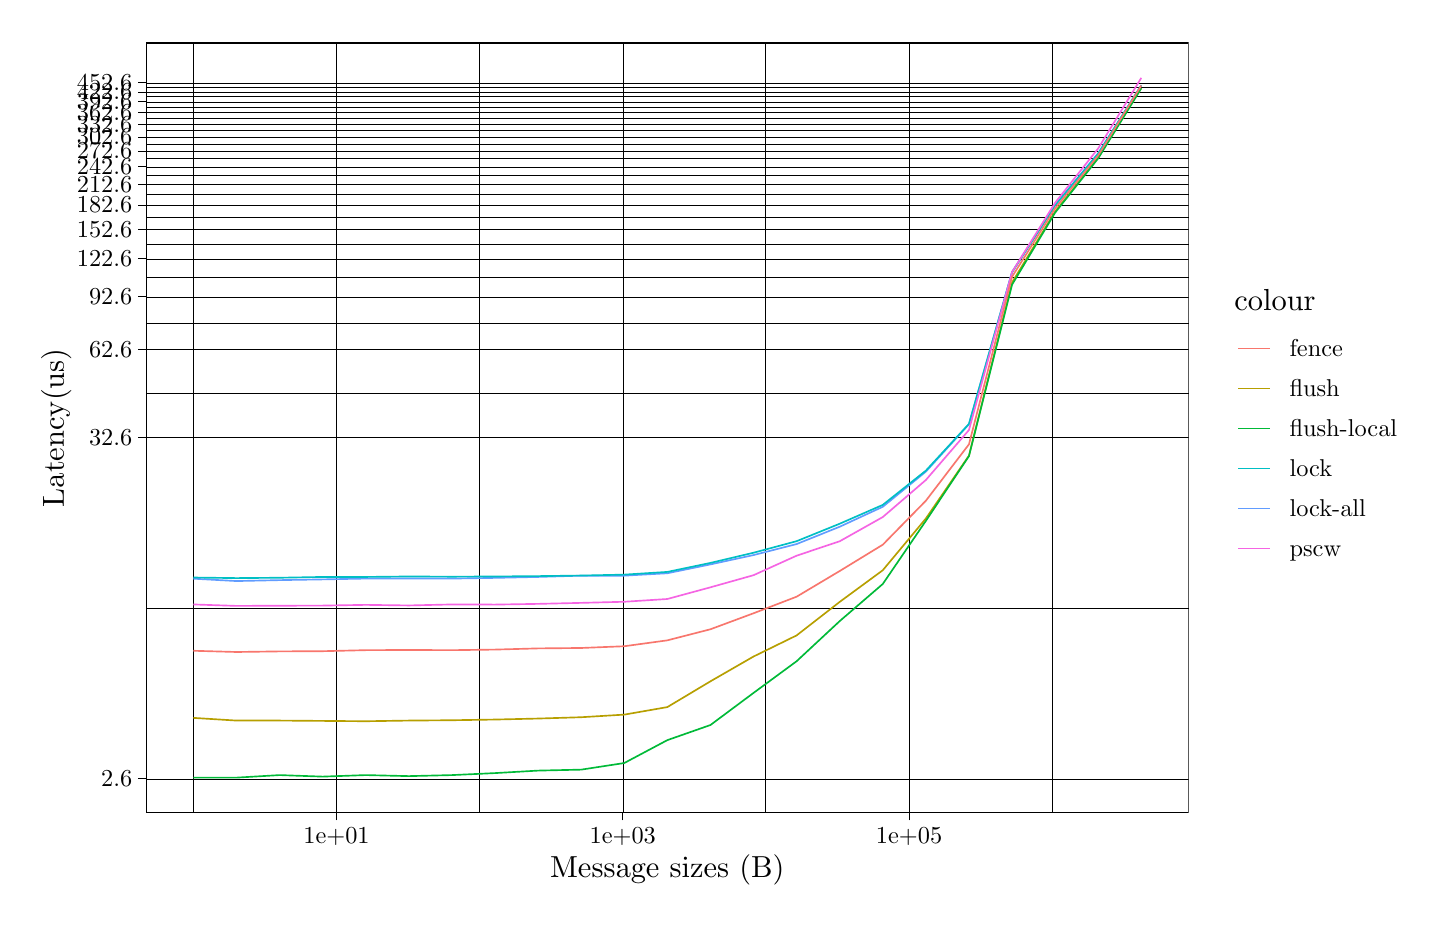
\begin{tikzpicture}[x=1pt,y=1pt]
\definecolor{fillColor}{RGB}{255,255,255}
\path[use as bounding box,fill=fillColor,fill opacity=0.00] (0,0) rectangle (505.89,314.37);
\begin{scope}
\path[clip] (  0.00,  0.00) rectangle (505.89,314.37);
\definecolor{drawColor}{RGB}{255,255,255}
\definecolor{fillColor}{RGB}{255,255,255}

\path[draw=drawColor,line width= 0.6pt,line join=round,line cap=round,fill=fillColor] (  0.00,  0.00) rectangle (505.89,314.37);
\end{scope}
\begin{scope}
\path[clip] ( 42.76, 30.72) rectangle (419.53,308.87);
\definecolor{fillColor}{RGB}{255,255,255}

\path[fill=fillColor] ( 42.76, 30.72) rectangle (419.53,308.87);
\definecolor{drawColor}{RGB}{0,0,0}

\path[draw=drawColor,line width= 0.0pt,line join=round] ( 42.76,104.63) --
	(419.53,104.63);

\path[draw=drawColor,line width= 0.0pt,line join=round] ( 42.76,182.16) --
	(419.53,182.16);

\path[draw=drawColor,line width= 0.0pt,line join=round] ( 42.76,207.61) --
	(419.53,207.61);

\path[draw=drawColor,line width= 0.0pt,line join=round] ( 42.76,223.99) --
	(419.53,223.99);

\path[draw=drawColor,line width= 0.0pt,line join=round] ( 42.76,236.16) --
	(419.53,236.16);

\path[draw=drawColor,line width= 0.0pt,line join=round] ( 42.76,245.87) --
	(419.53,245.87);

\path[draw=drawColor,line width= 0.0pt,line join=round] ( 42.76,253.96) --
	(419.53,253.96);

\path[draw=drawColor,line width= 0.0pt,line join=round] ( 42.76,260.88) --
	(419.53,260.88);

\path[draw=drawColor,line width= 0.0pt,line join=round] ( 42.76,266.94) --
	(419.53,266.94);

\path[draw=drawColor,line width= 0.0pt,line join=round] ( 42.76,272.32) --
	(419.53,272.32);

\path[draw=drawColor,line width= 0.0pt,line join=round] ( 42.76,277.17) --
	(419.53,277.17);

\path[draw=drawColor,line width= 0.0pt,line join=round] ( 42.76,281.58) --
	(419.53,281.58);

\path[draw=drawColor,line width= 0.0pt,line join=round] ( 42.76,285.62) --
	(419.53,285.62);

\path[draw=drawColor,line width= 0.0pt,line join=round] ( 42.76,289.36) --
	(419.53,289.36);

\path[draw=drawColor,line width= 0.0pt,line join=round] ( 42.76,292.82) --
	(419.53,292.82);

\path[draw=drawColor,line width= 0.0pt,line join=round] ( 59.89, 30.72) --
	( 59.89,308.87);

\path[draw=drawColor,line width= 0.0pt,line join=round] (163.32, 30.72) --
	(163.32,308.87);

\path[draw=drawColor,line width= 0.0pt,line join=round] (266.76, 30.72) --
	(266.76,308.87);

\path[draw=drawColor,line width= 0.0pt,line join=round] (370.20, 30.72) --
	(370.20,308.87);

\path[draw=drawColor,line width= 0.1pt,line join=round] ( 42.76, 42.99) --
	(419.53, 42.99);

\path[draw=drawColor,line width= 0.1pt,line join=round] ( 42.76,166.26) --
	(419.53,166.26);

\path[draw=drawColor,line width= 0.1pt,line join=round] ( 42.76,198.06) --
	(419.53,198.06);

\path[draw=drawColor,line width= 0.1pt,line join=round] ( 42.76,217.15) --
	(419.53,217.15);

\path[draw=drawColor,line width= 0.1pt,line join=round] ( 42.76,230.83) --
	(419.53,230.83);

\path[draw=drawColor,line width= 0.1pt,line join=round] ( 42.76,241.50) --
	(419.53,241.50);

\path[draw=drawColor,line width= 0.1pt,line join=round] ( 42.76,250.25) --
	(419.53,250.25);

\path[draw=drawColor,line width= 0.1pt,line join=round] ( 42.76,257.66) --
	(419.53,257.66);

\path[draw=drawColor,line width= 0.1pt,line join=round] ( 42.76,264.10) --
	(419.53,264.10);

\path[draw=drawColor,line width= 0.1pt,line join=round] ( 42.76,269.78) --
	(419.53,269.78);

\path[draw=drawColor,line width= 0.1pt,line join=round] ( 42.76,274.87) --
	(419.53,274.87);

\path[draw=drawColor,line width= 0.1pt,line join=round] ( 42.76,279.48) --
	(419.53,279.48);

\path[draw=drawColor,line width= 0.1pt,line join=round] ( 42.76,283.69) --
	(419.53,283.69);

\path[draw=drawColor,line width= 0.1pt,line join=round] ( 42.76,287.56) --
	(419.53,287.56);

\path[draw=drawColor,line width= 0.1pt,line join=round] ( 42.76,291.15) --
	(419.53,291.15);

\path[draw=drawColor,line width= 0.1pt,line join=round] ( 42.76,294.49) --
	(419.53,294.49);

\path[draw=drawColor,line width= 0.1pt,line join=round] (111.60, 30.72) --
	(111.60,308.87);

\path[draw=drawColor,line width= 0.1pt,line join=round] (215.04, 30.72) --
	(215.04,308.87);

\path[draw=drawColor,line width= 0.1pt,line join=round] (318.48, 30.72) --
	(318.48,308.87);
\definecolor{drawColor}{RGB}{97,156,255}

\path[draw=drawColor,line width= 0.6pt,line join=round] ( 59.89,115.26) --
	( 75.45,114.40) --
	( 91.02,114.74) --
	(106.59,115.00) --
	(122.16,115.30) --
	(137.73,115.30) --
	(153.30,115.30) --
	(168.87,115.55) --
	(184.44,115.89) --
	(200.01,116.35) --
	(215.58,116.35) --
	(231.14,117.22) --
	(246.71,120.42) --
	(262.28,123.79) --
	(277.85,127.77) --
	(293.42,134.03) --
	(308.99,141.24) --
	(324.56,153.94) --
	(340.13,171.08) --
	(355.70,226.09) --
	(371.27,250.28) --
	(386.83,268.98) --
	(402.40,293.57);
\definecolor{drawColor}{RGB}{0,191,196}

\path[draw=drawColor,line width= 0.6pt,line join=round] ( 59.89,115.68) --
	( 75.45,115.47) --
	( 91.02,115.60) --
	(106.59,115.89) --
	(122.16,115.89) --
	(137.73,116.06) --
	(153.30,115.98) --
	(168.87,116.06) --
	(184.44,116.19) --
	(200.01,116.39) --
	(215.58,116.73) --
	(231.14,117.71) --
	(246.71,120.96) --
	(262.28,124.64) --
	(277.85,128.81) --
	(293.42,135.12) --
	(308.99,141.93) --
	(324.56,154.31) --
	(340.13,171.20) --
	(355.70,225.95) --
	(371.27,250.18) --
	(386.83,268.88) --
	(402.40,293.50);
\definecolor{drawColor}{RGB}{183,159,0}

\path[draw=drawColor,line width= 0.6pt,line join=round] ( 59.89, 64.96) --
	( 75.45, 63.99) --
	( 91.02, 63.99) --
	(106.59, 63.87) --
	(122.16, 63.75) --
	(137.73, 63.99) --
	(153.30, 64.11) --
	(168.87, 64.36) --
	(184.44, 64.72) --
	(200.01, 65.20) --
	(215.58, 66.14) --
	(231.14, 68.86) --
	(246.71, 78.17) --
	(262.28, 87.13) --
	(277.85, 94.76) --
	(293.42,106.87) --
	(308.99,118.31) --
	(324.56,137.01) --
	(340.13,159.74) --
	(355.70,222.30) --
	(371.27,247.94) --
	(386.83,267.41) --
	(402.40,292.60);
\definecolor{drawColor}{RGB}{0,186,56}

\path[draw=drawColor,line width= 0.6pt,line join=round] ( 59.89, 43.37) --
	( 75.45, 43.37) --
	( 91.02, 44.29) --
	(106.59, 43.74) --
	(122.16, 44.29) --
	(137.73, 43.92) --
	(153.30, 44.29) --
	(168.87, 45.01) --
	(184.44, 45.91) --
	(200.01, 46.26) --
	(215.58, 48.65) --
	(231.14, 56.92) --
	(246.71, 62.38) --
	(262.28, 73.98) --
	(277.85, 85.43) --
	(293.42, 99.93) --
	(308.99,113.35) --
	(324.56,136.16) --
	(340.13,159.55) --
	(355.70,221.49) --
	(371.27,247.53) --
	(386.83,267.16) --
	(402.40,292.48);
\definecolor{drawColor}{RGB}{245,100,227}

\path[draw=drawColor,line width= 0.6pt,line join=round] ( 59.89,105.95) --
	( 75.45,105.43) --
	( 91.02,105.49) --
	(106.59,105.54) --
	(122.16,105.80) --
	(137.73,105.59) --
	(153.30,105.95) --
	(168.87,105.90) --
	(184.44,106.16) --
	(200.01,106.52) --
	(215.58,106.92) --
	(231.14,107.92) --
	(246.71,112.14) --
	(262.28,116.52) --
	(277.85,123.57) --
	(293.42,128.78) --
	(308.99,137.53) --
	(324.56,150.92) --
	(340.13,168.98) --
	(355.70,226.05) --
	(371.27,251.12) --
	(386.83,270.73) --
	(402.40,296.23);
\definecolor{drawColor}{RGB}{248,118,109}

\path[draw=drawColor,line width= 0.6pt,line join=round] ( 59.89, 89.21) --
	( 75.45, 88.77) --
	( 91.02, 88.99) --
	(106.59, 89.06) --
	(122.16, 89.43) --
	(137.73, 89.50) --
	(153.30, 89.43) --
	(168.87, 89.64) --
	(184.44, 90.07) --
	(200.01, 90.22) --
	(215.58, 90.85) --
	(231.14, 92.98) --
	(246.71, 96.98) --
	(262.28,102.76) --
	(277.85,108.75) --
	(293.42,118.03) --
	(308.99,127.54) --
	(324.56,143.43) --
	(340.13,163.81) --
	(355.70,224.35) --
	(371.27,249.11) --
	(386.83,268.21) --
	(402.40,293.47);
\definecolor{drawColor}{RGB}{0,0,0}

\path[draw=drawColor,line width= 0.6pt,line join=round,line cap=round] ( 42.76, 30.72) rectangle (419.53,308.87);
\end{scope}
\begin{scope}
\path[clip] (  0.00,  0.00) rectangle (505.89,314.37);
\definecolor{drawColor}{RGB}{0,0,0}

\node[text=drawColor,anchor=base west,inner sep=0pt, outer sep=0pt, scale=  0.88] at ( 26.57, 40.17) {2.6};

\node[text=drawColor,anchor=base west,inner sep=0pt, outer sep=0pt, scale=  0.88] at ( 22.17,163.44) {32.6};

\node[text=drawColor,anchor=base west,inner sep=0pt, outer sep=0pt, scale=  0.88] at ( 22.17,195.24) {62.6};

\node[text=drawColor,anchor=base west,inner sep=0pt, outer sep=0pt, scale=  0.88] at ( 22.17,214.33) {92.6};

\node[text=drawColor,anchor=base west,inner sep=0pt, outer sep=0pt, scale=  0.88] at ( 17.77,228.01) {122.6};

\node[text=drawColor,anchor=base west,inner sep=0pt, outer sep=0pt, scale=  0.88] at ( 17.77,238.68) {152.6};

\node[text=drawColor,anchor=base west,inner sep=0pt, outer sep=0pt, scale=  0.88] at ( 17.77,247.43) {182.6};

\node[text=drawColor,anchor=base west,inner sep=0pt, outer sep=0pt, scale=  0.88] at ( 17.77,254.84) {212.6};

\node[text=drawColor,anchor=base west,inner sep=0pt, outer sep=0pt, scale=  0.88] at ( 17.77,261.27) {242.6};

\node[text=drawColor,anchor=base west,inner sep=0pt, outer sep=0pt, scale=  0.88] at ( 17.77,266.96) {272.6};

\node[text=drawColor,anchor=base west,inner sep=0pt, outer sep=0pt, scale=  0.88] at ( 17.77,272.05) {302.6};

\node[text=drawColor,anchor=base west,inner sep=0pt, outer sep=0pt, scale=  0.88] at ( 17.77,276.65) {332.6};

\node[text=drawColor,anchor=base west,inner sep=0pt, outer sep=0pt, scale=  0.88] at ( 17.77,280.86) {362.6};

\node[text=drawColor,anchor=base west,inner sep=0pt, outer sep=0pt, scale=  0.88] at ( 17.77,284.74) {392.6};

\node[text=drawColor,anchor=base west,inner sep=0pt, outer sep=0pt, scale=  0.88] at ( 17.77,288.33) {422.6};

\node[text=drawColor,anchor=base west,inner sep=0pt, outer sep=0pt, scale=  0.88] at ( 17.77,291.67) {452.6};
\end{scope}
\begin{scope}
\path[clip] (  0.00,  0.00) rectangle (505.89,314.37);
\definecolor{drawColor}{RGB}{0,0,0}

\path[draw=drawColor,line width= 0.3pt,line join=round] ( 40.01, 42.99) --
	( 42.76, 42.99);

\path[draw=drawColor,line width= 0.3pt,line join=round] ( 40.01,166.26) --
	( 42.76,166.26);

\path[draw=drawColor,line width= 0.3pt,line join=round] ( 40.01,198.06) --
	( 42.76,198.06);

\path[draw=drawColor,line width= 0.3pt,line join=round] ( 40.01,217.15) --
	( 42.76,217.15);

\path[draw=drawColor,line width= 0.3pt,line join=round] ( 40.01,230.83) --
	( 42.76,230.83);

\path[draw=drawColor,line width= 0.3pt,line join=round] ( 40.01,241.50) --
	( 42.76,241.50);

\path[draw=drawColor,line width= 0.3pt,line join=round] ( 40.01,250.25) --
	( 42.76,250.25);

\path[draw=drawColor,line width= 0.3pt,line join=round] ( 40.01,257.66) --
	( 42.76,257.66);

\path[draw=drawColor,line width= 0.3pt,line join=round] ( 40.01,264.10) --
	( 42.76,264.10);

\path[draw=drawColor,line width= 0.3pt,line join=round] ( 40.01,269.78) --
	( 42.76,269.78);

\path[draw=drawColor,line width= 0.3pt,line join=round] ( 40.01,274.87) --
	( 42.76,274.87);

\path[draw=drawColor,line width= 0.3pt,line join=round] ( 40.01,279.48) --
	( 42.76,279.48);

\path[draw=drawColor,line width= 0.3pt,line join=round] ( 40.01,283.69) --
	( 42.76,283.69);

\path[draw=drawColor,line width= 0.3pt,line join=round] ( 40.01,287.56) --
	( 42.76,287.56);

\path[draw=drawColor,line width= 0.3pt,line join=round] ( 40.01,291.15) --
	( 42.76,291.15);

\path[draw=drawColor,line width= 0.3pt,line join=round] ( 40.01,294.49) --
	( 42.76,294.49);
\end{scope}
\begin{scope}
\path[clip] (  0.00,  0.00) rectangle (505.89,314.37);
\definecolor{drawColor}{RGB}{0,0,0}

\path[draw=drawColor,line width= 0.3pt,line join=round] (111.60, 27.97) --
	(111.60, 30.72);

\path[draw=drawColor,line width= 0.3pt,line join=round] (215.04, 27.97) --
	(215.04, 30.72);

\path[draw=drawColor,line width= 0.3pt,line join=round] (318.48, 27.97) --
	(318.48, 30.72);
\end{scope}
\begin{scope}
\path[clip] (  0.00,  0.00) rectangle (505.89,314.37);
\definecolor{drawColor}{RGB}{0,0,0}

\node[text=drawColor,anchor=base,inner sep=0pt, outer sep=0pt, scale=  0.88] at (111.60, 19.71) {1e+01};

\node[text=drawColor,anchor=base,inner sep=0pt, outer sep=0pt, scale=  0.88] at (215.04, 19.71) {1e+03};

\node[text=drawColor,anchor=base,inner sep=0pt, outer sep=0pt, scale=  0.88] at (318.48, 19.71) {1e+05};
\end{scope}
\begin{scope}
\path[clip] (  0.00,  0.00) rectangle (505.89,314.37);
\definecolor{drawColor}{RGB}{0,0,0}

\node[text=drawColor,anchor=base,inner sep=0pt, outer sep=0pt, scale=  1.10] at (231.14,  7.44) {Message sizes (B)};
\end{scope}
\begin{scope}
\path[clip] (  0.00,  0.00) rectangle (505.89,314.37);
\definecolor{drawColor}{RGB}{0,0,0}

\node[text=drawColor,rotate= 90.00,anchor=base,inner sep=0pt, outer sep=0pt, scale=  1.10] at ( 13.08,169.80) {Latency(us)};
\end{scope}
\begin{scope}
\path[clip] (  0.00,  0.00) rectangle (505.89,314.37);
\definecolor{fillColor}{RGB}{255,255,255}

\path[fill=fillColor] (430.53,113.43) rectangle (500.39,226.17);
\end{scope}
\begin{scope}
\path[clip] (  0.00,  0.00) rectangle (505.89,314.37);
\definecolor{drawColor}{RGB}{0,0,0}

\node[text=drawColor,anchor=base west,inner sep=0pt, outer sep=0pt, scale=  1.10] at (436.03,212.12) {colour};
\end{scope}
\begin{scope}
\path[clip] (  0.00,  0.00) rectangle (505.89,314.37);
\definecolor{fillColor}{RGB}{255,255,255}

\path[fill=fillColor] (436.03,191.20) rectangle (450.48,205.65);
\end{scope}
\begin{scope}
\path[clip] (  0.00,  0.00) rectangle (505.89,314.37);
\definecolor{drawColor}{RGB}{248,118,109}

\path[draw=drawColor,line width= 0.6pt,line join=round] (437.48,198.42) -- (449.04,198.42);
\end{scope}
\begin{scope}
\path[clip] (  0.00,  0.00) rectangle (505.89,314.37);
\definecolor{drawColor}{RGB}{248,118,109}

\path[draw=drawColor,line width= 0.6pt,line join=round] (437.48,198.42) -- (449.04,198.42);
\end{scope}
\begin{scope}
\path[clip] (  0.00,  0.00) rectangle (505.89,314.37);
\definecolor{drawColor}{RGB}{248,118,109}

\path[draw=drawColor,line width= 0.6pt,line join=round] (437.48,198.42) -- (449.04,198.42);
\end{scope}
\begin{scope}
\path[clip] (  0.00,  0.00) rectangle (505.89,314.37);
\definecolor{drawColor}{RGB}{248,118,109}

\path[draw=drawColor,line width= 0.6pt,line join=round] (437.48,198.42) -- (449.04,198.42);
\end{scope}
\begin{scope}
\path[clip] (  0.00,  0.00) rectangle (505.89,314.37);
\definecolor{drawColor}{RGB}{248,118,109}

\path[draw=drawColor,line width= 0.6pt,line join=round] (437.48,198.42) -- (449.04,198.42);
\end{scope}
\begin{scope}
\path[clip] (  0.00,  0.00) rectangle (505.89,314.37);
\definecolor{drawColor}{RGB}{248,118,109}

\path[draw=drawColor,line width= 0.6pt,line join=round] (437.48,198.42) -- (449.04,198.42);
\end{scope}
\begin{scope}
\path[clip] (  0.00,  0.00) rectangle (505.89,314.37);
\definecolor{fillColor}{RGB}{255,255,255}

\path[fill=fillColor] (436.03,176.74) rectangle (450.48,191.20);
\end{scope}
\begin{scope}
\path[clip] (  0.00,  0.00) rectangle (505.89,314.37);
\definecolor{drawColor}{RGB}{183,159,0}

\path[draw=drawColor,line width= 0.6pt,line join=round] (437.48,183.97) -- (449.04,183.97);
\end{scope}
\begin{scope}
\path[clip] (  0.00,  0.00) rectangle (505.89,314.37);
\definecolor{drawColor}{RGB}{183,159,0}

\path[draw=drawColor,line width= 0.6pt,line join=round] (437.48,183.97) -- (449.04,183.97);
\end{scope}
\begin{scope}
\path[clip] (  0.00,  0.00) rectangle (505.89,314.37);
\definecolor{drawColor}{RGB}{183,159,0}

\path[draw=drawColor,line width= 0.6pt,line join=round] (437.48,183.97) -- (449.04,183.97);
\end{scope}
\begin{scope}
\path[clip] (  0.00,  0.00) rectangle (505.89,314.37);
\definecolor{drawColor}{RGB}{183,159,0}

\path[draw=drawColor,line width= 0.6pt,line join=round] (437.48,183.97) -- (449.04,183.97);
\end{scope}
\begin{scope}
\path[clip] (  0.00,  0.00) rectangle (505.89,314.37);
\definecolor{drawColor}{RGB}{183,159,0}

\path[draw=drawColor,line width= 0.6pt,line join=round] (437.48,183.97) -- (449.04,183.97);
\end{scope}
\begin{scope}
\path[clip] (  0.00,  0.00) rectangle (505.89,314.37);
\definecolor{drawColor}{RGB}{183,159,0}

\path[draw=drawColor,line width= 0.6pt,line join=round] (437.48,183.97) -- (449.04,183.97);
\end{scope}
\begin{scope}
\path[clip] (  0.00,  0.00) rectangle (505.89,314.37);
\definecolor{fillColor}{RGB}{255,255,255}

\path[fill=fillColor] (436.03,162.29) rectangle (450.48,176.74);
\end{scope}
\begin{scope}
\path[clip] (  0.00,  0.00) rectangle (505.89,314.37);
\definecolor{drawColor}{RGB}{0,186,56}

\path[draw=drawColor,line width= 0.6pt,line join=round] (437.48,169.52) -- (449.04,169.52);
\end{scope}
\begin{scope}
\path[clip] (  0.00,  0.00) rectangle (505.89,314.37);
\definecolor{drawColor}{RGB}{0,186,56}

\path[draw=drawColor,line width= 0.6pt,line join=round] (437.48,169.52) -- (449.04,169.52);
\end{scope}
\begin{scope}
\path[clip] (  0.00,  0.00) rectangle (505.89,314.37);
\definecolor{drawColor}{RGB}{0,186,56}

\path[draw=drawColor,line width= 0.6pt,line join=round] (437.48,169.52) -- (449.04,169.52);
\end{scope}
\begin{scope}
\path[clip] (  0.00,  0.00) rectangle (505.89,314.37);
\definecolor{drawColor}{RGB}{0,186,56}

\path[draw=drawColor,line width= 0.6pt,line join=round] (437.48,169.52) -- (449.04,169.52);
\end{scope}
\begin{scope}
\path[clip] (  0.00,  0.00) rectangle (505.89,314.37);
\definecolor{drawColor}{RGB}{0,186,56}

\path[draw=drawColor,line width= 0.6pt,line join=round] (437.48,169.52) -- (449.04,169.52);
\end{scope}
\begin{scope}
\path[clip] (  0.00,  0.00) rectangle (505.89,314.37);
\definecolor{drawColor}{RGB}{0,186,56}

\path[draw=drawColor,line width= 0.6pt,line join=round] (437.48,169.52) -- (449.04,169.52);
\end{scope}
\begin{scope}
\path[clip] (  0.00,  0.00) rectangle (505.89,314.37);
\definecolor{fillColor}{RGB}{255,255,255}

\path[fill=fillColor] (436.03,147.84) rectangle (450.48,162.29);
\end{scope}
\begin{scope}
\path[clip] (  0.00,  0.00) rectangle (505.89,314.37);
\definecolor{drawColor}{RGB}{0,191,196}

\path[draw=drawColor,line width= 0.6pt,line join=round] (437.48,155.06) -- (449.04,155.06);
\end{scope}
\begin{scope}
\path[clip] (  0.00,  0.00) rectangle (505.89,314.37);
\definecolor{drawColor}{RGB}{0,191,196}

\path[draw=drawColor,line width= 0.6pt,line join=round] (437.48,155.06) -- (449.04,155.06);
\end{scope}
\begin{scope}
\path[clip] (  0.00,  0.00) rectangle (505.89,314.37);
\definecolor{drawColor}{RGB}{0,191,196}

\path[draw=drawColor,line width= 0.6pt,line join=round] (437.48,155.06) -- (449.04,155.06);
\end{scope}
\begin{scope}
\path[clip] (  0.00,  0.00) rectangle (505.89,314.37);
\definecolor{drawColor}{RGB}{0,191,196}

\path[draw=drawColor,line width= 0.6pt,line join=round] (437.48,155.06) -- (449.04,155.06);
\end{scope}
\begin{scope}
\path[clip] (  0.00,  0.00) rectangle (505.89,314.37);
\definecolor{drawColor}{RGB}{0,191,196}

\path[draw=drawColor,line width= 0.6pt,line join=round] (437.48,155.06) -- (449.04,155.06);
\end{scope}
\begin{scope}
\path[clip] (  0.00,  0.00) rectangle (505.89,314.37);
\definecolor{drawColor}{RGB}{0,191,196}

\path[draw=drawColor,line width= 0.6pt,line join=round] (437.48,155.06) -- (449.04,155.06);
\end{scope}
\begin{scope}
\path[clip] (  0.00,  0.00) rectangle (505.89,314.37);
\definecolor{fillColor}{RGB}{255,255,255}

\path[fill=fillColor] (436.03,133.38) rectangle (450.48,147.84);
\end{scope}
\begin{scope}
\path[clip] (  0.00,  0.00) rectangle (505.89,314.37);
\definecolor{drawColor}{RGB}{97,156,255}

\path[draw=drawColor,line width= 0.6pt,line join=round] (437.48,140.61) -- (449.04,140.61);
\end{scope}
\begin{scope}
\path[clip] (  0.00,  0.00) rectangle (505.89,314.37);
\definecolor{drawColor}{RGB}{97,156,255}

\path[draw=drawColor,line width= 0.6pt,line join=round] (437.48,140.61) -- (449.04,140.61);
\end{scope}
\begin{scope}
\path[clip] (  0.00,  0.00) rectangle (505.89,314.37);
\definecolor{drawColor}{RGB}{97,156,255}

\path[draw=drawColor,line width= 0.6pt,line join=round] (437.48,140.61) -- (449.04,140.61);
\end{scope}
\begin{scope}
\path[clip] (  0.00,  0.00) rectangle (505.89,314.37);
\definecolor{drawColor}{RGB}{97,156,255}

\path[draw=drawColor,line width= 0.6pt,line join=round] (437.48,140.61) -- (449.04,140.61);
\end{scope}
\begin{scope}
\path[clip] (  0.00,  0.00) rectangle (505.89,314.37);
\definecolor{drawColor}{RGB}{97,156,255}

\path[draw=drawColor,line width= 0.6pt,line join=round] (437.48,140.61) -- (449.04,140.61);
\end{scope}
\begin{scope}
\path[clip] (  0.00,  0.00) rectangle (505.89,314.37);
\definecolor{drawColor}{RGB}{97,156,255}

\path[draw=drawColor,line width= 0.6pt,line join=round] (437.48,140.61) -- (449.04,140.61);
\end{scope}
\begin{scope}
\path[clip] (  0.00,  0.00) rectangle (505.89,314.37);
\definecolor{fillColor}{RGB}{255,255,255}

\path[fill=fillColor] (436.03,118.93) rectangle (450.48,133.38);
\end{scope}
\begin{scope}
\path[clip] (  0.00,  0.00) rectangle (505.89,314.37);
\definecolor{drawColor}{RGB}{245,100,227}

\path[draw=drawColor,line width= 0.6pt,line join=round] (437.48,126.15) -- (449.04,126.15);
\end{scope}
\begin{scope}
\path[clip] (  0.00,  0.00) rectangle (505.89,314.37);
\definecolor{drawColor}{RGB}{245,100,227}

\path[draw=drawColor,line width= 0.6pt,line join=round] (437.48,126.15) -- (449.04,126.15);
\end{scope}
\begin{scope}
\path[clip] (  0.00,  0.00) rectangle (505.89,314.37);
\definecolor{drawColor}{RGB}{245,100,227}

\path[draw=drawColor,line width= 0.6pt,line join=round] (437.48,126.15) -- (449.04,126.15);
\end{scope}
\begin{scope}
\path[clip] (  0.00,  0.00) rectangle (505.89,314.37);
\definecolor{drawColor}{RGB}{245,100,227}

\path[draw=drawColor,line width= 0.6pt,line join=round] (437.48,126.15) -- (449.04,126.15);
\end{scope}
\begin{scope}
\path[clip] (  0.00,  0.00) rectangle (505.89,314.37);
\definecolor{drawColor}{RGB}{245,100,227}

\path[draw=drawColor,line width= 0.6pt,line join=round] (437.48,126.15) -- (449.04,126.15);
\end{scope}
\begin{scope}
\path[clip] (  0.00,  0.00) rectangle (505.89,314.37);
\definecolor{drawColor}{RGB}{245,100,227}

\path[draw=drawColor,line width= 0.6pt,line join=round] (437.48,126.15) -- (449.04,126.15);
\end{scope}
\begin{scope}
\path[clip] (  0.00,  0.00) rectangle (505.89,314.37);
\definecolor{drawColor}{RGB}{0,0,0}

\node[text=drawColor,anchor=base west,inner sep=0pt, outer sep=0pt, scale=  0.88] at (455.98,195.39) {fence};
\end{scope}
\begin{scope}
\path[clip] (  0.00,  0.00) rectangle (505.89,314.37);
\definecolor{drawColor}{RGB}{0,0,0}

\node[text=drawColor,anchor=base west,inner sep=0pt, outer sep=0pt, scale=  0.88] at (455.98,180.94) {flush};
\end{scope}
\begin{scope}
\path[clip] (  0.00,  0.00) rectangle (505.89,314.37);
\definecolor{drawColor}{RGB}{0,0,0}

\node[text=drawColor,anchor=base west,inner sep=0pt, outer sep=0pt, scale=  0.88] at (455.98,166.49) {flush-local};
\end{scope}
\begin{scope}
\path[clip] (  0.00,  0.00) rectangle (505.89,314.37);
\definecolor{drawColor}{RGB}{0,0,0}

\node[text=drawColor,anchor=base west,inner sep=0pt, outer sep=0pt, scale=  0.88] at (455.98,152.03) {lock};
\end{scope}
\begin{scope}
\path[clip] (  0.00,  0.00) rectangle (505.89,314.37);
\definecolor{drawColor}{RGB}{0,0,0}

\node[text=drawColor,anchor=base west,inner sep=0pt, outer sep=0pt, scale=  0.88] at (455.98,137.58) {lock-all};
\end{scope}
\begin{scope}
\path[clip] (  0.00,  0.00) rectangle (505.89,314.37);
\definecolor{drawColor}{RGB}{0,0,0}

\node[text=drawColor,anchor=base west,inner sep=0pt, outer sep=0pt, scale=  0.88] at (455.98,123.12) {pscw};
\end{scope}
\end{tikzpicture}

	\caption{2 nodes, get latency, gpu-gpu, window create, sync algorithm comparisons}
\end{figure}

\begin{figure}
	% Created by tikzDevice version 0.10.1 on 2020-02-15 15:55:10
% !TEX encoding = UTF-8 Unicode
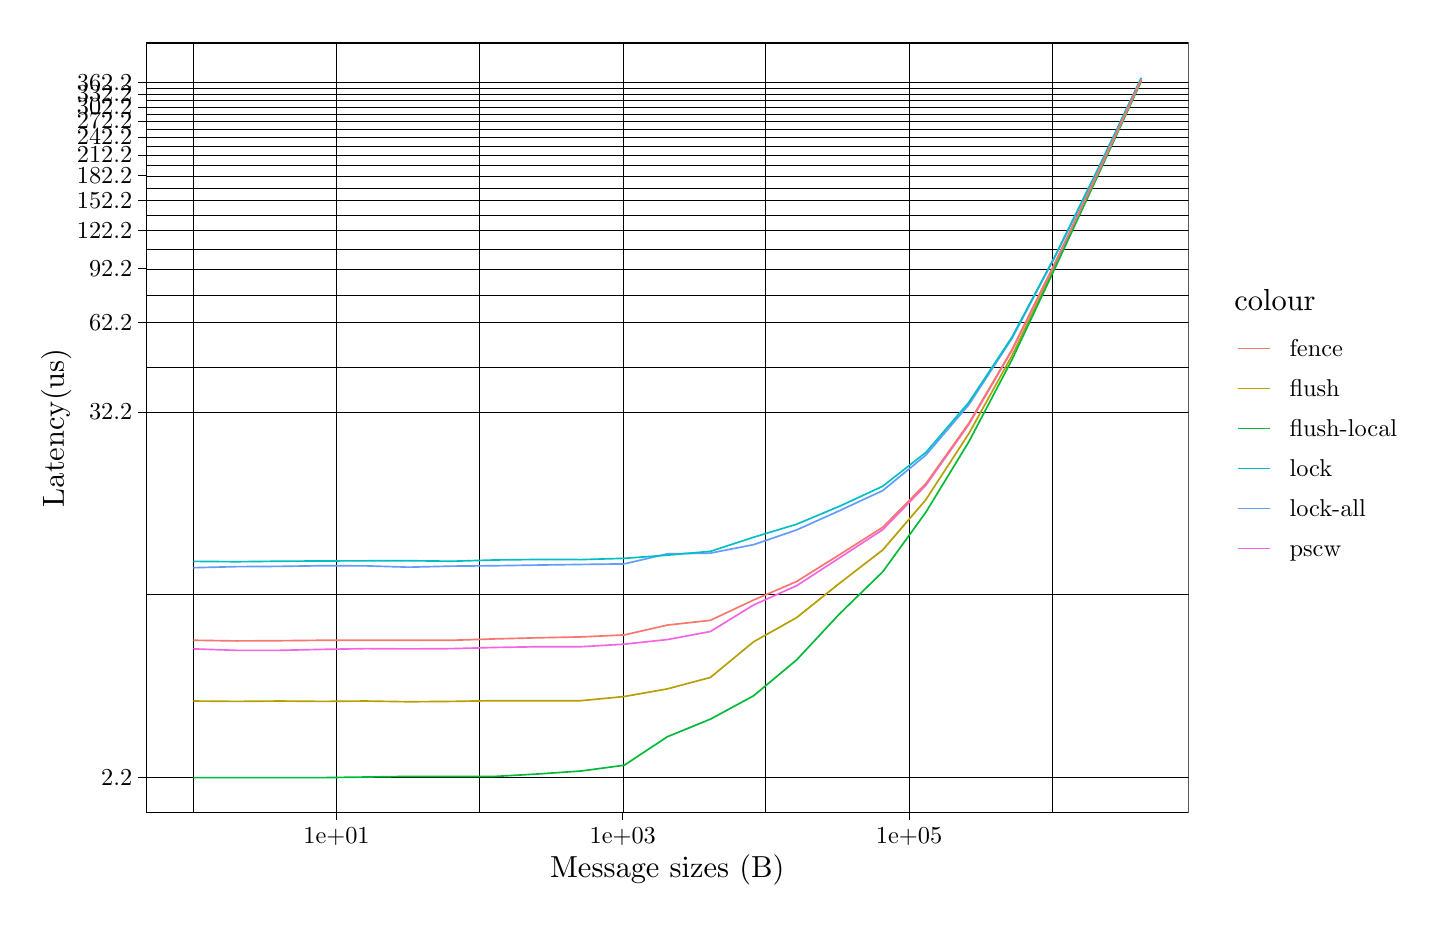
\begin{tikzpicture}[x=1pt,y=1pt]
\definecolor{fillColor}{RGB}{255,255,255}
\path[use as bounding box,fill=fillColor,fill opacity=0.00] (0,0) rectangle (505.89,314.37);
\begin{scope}
\path[clip] (  0.00,  0.00) rectangle (505.89,314.37);
\definecolor{drawColor}{RGB}{255,255,255}
\definecolor{fillColor}{RGB}{255,255,255}

\path[draw=drawColor,line width= 0.6pt,line join=round,line cap=round,fill=fillColor] (  0.00,  0.00) rectangle (505.89,314.37);
\end{scope}
\begin{scope}
\path[clip] ( 42.76, 30.72) rectangle (419.53,308.87);
\definecolor{fillColor}{RGB}{255,255,255}

\path[fill=fillColor] ( 42.76, 30.72) rectangle (419.53,308.87);
\definecolor{drawColor}{RGB}{0,0,0}

\path[draw=drawColor,line width= 0.0pt,line join=round] ( 42.76,109.43) --
	(419.53,109.43);

\path[draw=drawColor,line width= 0.0pt,line join=round] ( 42.76,191.70) --
	(419.53,191.70);

\path[draw=drawColor,line width= 0.0pt,line join=round] ( 42.76,217.60) --
	(419.53,217.60);

\path[draw=drawColor,line width= 0.0pt,line join=round] ( 42.76,234.22) --
	(419.53,234.22);

\path[draw=drawColor,line width= 0.0pt,line join=round] ( 42.76,246.56) --
	(419.53,246.56);

\path[draw=drawColor,line width= 0.0pt,line join=round] ( 42.76,256.39) --
	(419.53,256.39);

\path[draw=drawColor,line width= 0.0pt,line join=round] ( 42.76,264.57) --
	(419.53,264.57);

\path[draw=drawColor,line width= 0.0pt,line join=round] ( 42.76,271.58) --
	(419.53,271.58);

\path[draw=drawColor,line width= 0.0pt,line join=round] ( 42.76,277.71) --
	(419.53,277.71);

\path[draw=drawColor,line width= 0.0pt,line join=round] ( 42.76,283.16) --
	(419.53,283.16);

\path[draw=drawColor,line width= 0.0pt,line join=round] ( 42.76,288.06) --
	(419.53,288.06);

\path[draw=drawColor,line width= 0.0pt,line join=round] ( 42.76,292.52) --
	(419.53,292.52);

\path[draw=drawColor,line width= 0.0pt,line join=round] ( 59.89, 30.72) --
	( 59.89,308.87);

\path[draw=drawColor,line width= 0.0pt,line join=round] (163.32, 30.72) --
	(163.32,308.87);

\path[draw=drawColor,line width= 0.0pt,line join=round] (266.76, 30.72) --
	(266.76,308.87);

\path[draw=drawColor,line width= 0.0pt,line join=round] (370.20, 30.72) --
	(370.20,308.87);

\path[draw=drawColor,line width= 0.1pt,line join=round] ( 42.76, 43.37) --
	(419.53, 43.37);

\path[draw=drawColor,line width= 0.1pt,line join=round] ( 42.76,175.49) --
	(419.53,175.49);

\path[draw=drawColor,line width= 0.1pt,line join=round] ( 42.76,207.91) --
	(419.53,207.91);

\path[draw=drawColor,line width= 0.1pt,line join=round] ( 42.76,227.29) --
	(419.53,227.29);

\path[draw=drawColor,line width= 0.1pt,line join=round] ( 42.76,241.16) --
	(419.53,241.16);

\path[draw=drawColor,line width= 0.1pt,line join=round] ( 42.76,251.96) --
	(419.53,251.96);

\path[draw=drawColor,line width= 0.1pt,line join=round] ( 42.76,260.82) --
	(419.53,260.82);

\path[draw=drawColor,line width= 0.1pt,line join=round] ( 42.76,268.33) --
	(419.53,268.33);

\path[draw=drawColor,line width= 0.1pt,line join=round] ( 42.76,274.84) --
	(419.53,274.84);

\path[draw=drawColor,line width= 0.1pt,line join=round] ( 42.76,280.59) --
	(419.53,280.59);

\path[draw=drawColor,line width= 0.1pt,line join=round] ( 42.76,285.73) --
	(419.53,285.73);

\path[draw=drawColor,line width= 0.1pt,line join=round] ( 42.76,290.39) --
	(419.53,290.39);

\path[draw=drawColor,line width= 0.1pt,line join=round] ( 42.76,294.65) --
	(419.53,294.65);

\path[draw=drawColor,line width= 0.1pt,line join=round] (111.60, 30.72) --
	(111.60,308.87);

\path[draw=drawColor,line width= 0.1pt,line join=round] (215.04, 30.72) --
	(215.04,308.87);

\path[draw=drawColor,line width= 0.1pt,line join=round] (318.48, 30.72) --
	(318.48,308.87);
\definecolor{drawColor}{RGB}{97,156,255}

\path[draw=drawColor,line width= 0.6pt,line join=round] ( 59.89,119.23) --
	( 75.45,119.61) --
	( 91.02,119.71) --
	(106.59,119.94) --
	(122.16,119.89) --
	(137.73,119.42) --
	(153.30,119.80) --
	(168.87,119.94) --
	(184.44,120.18) --
	(200.01,120.41) --
	(215.58,120.60) --
	(231.14,124.24) --
	(246.71,124.50) --
	(262.28,127.55) --
	(277.85,132.87) --
	(293.42,139.87) --
	(308.99,147.10) --
	(324.56,159.92) --
	(340.13,178.18) --
	(355.70,202.12) --
	(371.27,231.66) --
	(386.83,263.34) --
	(402.40,296.19);
\definecolor{drawColor}{RGB}{0,191,196}

\path[draw=drawColor,line width= 0.6pt,line join=round] ( 59.89,121.52) --
	( 75.45,121.39) --
	( 91.02,121.57) --
	(106.59,121.66) --
	(122.16,121.71) --
	(137.73,121.75) --
	(153.30,121.57) --
	(168.87,122.02) --
	(184.44,122.20) --
	(200.01,122.16) --
	(215.58,122.61) --
	(231.14,123.76) --
	(246.71,125.14) --
	(262.28,130.22) --
	(277.85,134.94) --
	(293.42,141.46) --
	(308.99,148.68) --
	(324.56,160.88) --
	(340.13,179.04) --
	(355.70,202.60) --
	(371.27,231.94) --
	(386.83,263.46) --
	(402.40,296.23);
\definecolor{drawColor}{RGB}{183,159,0}

\path[draw=drawColor,line width= 0.6pt,line join=round] ( 59.89, 71.05) --
	( 75.45, 70.92) --
	( 91.02, 71.05) --
	(106.59, 70.92) --
	(122.16, 71.05) --
	(137.73, 70.79) --
	(153.30, 70.92) --
	(168.87, 71.18) --
	(184.44, 71.18) --
	(200.01, 71.18) --
	(215.58, 72.68) --
	(231.14, 75.44) --
	(246.71, 79.58) --
	(262.28, 92.44) --
	(277.85,101.19) --
	(293.42,113.65) --
	(308.99,125.65) --
	(324.56,143.81) --
	(340.13,167.76) --
	(355.70,195.90) --
	(371.27,228.35) --
	(386.83,261.58) --
	(402.40,295.26);
\definecolor{drawColor}{RGB}{0,186,56}

\path[draw=drawColor,line width= 0.6pt,line join=round] ( 59.89, 43.37) --
	( 75.45, 43.37) --
	( 91.02, 43.37) --
	(106.59, 43.37) --
	(122.16, 43.59) --
	(137.73, 43.81) --
	(153.30, 43.81) --
	(168.87, 43.81) --
	(184.44, 44.69) --
	(200.01, 45.77) --
	(215.58, 47.86) --
	(231.14, 58.14) --
	(246.71, 64.51) --
	(262.28, 72.93) --
	(277.85, 85.91) --
	(293.42,102.62) --
	(308.99,117.77) --
	(324.56,139.27) --
	(340.13,164.81) --
	(355.70,194.44) --
	(371.27,227.57) --
	(386.83,261.20) --
	(402.40,295.07);
\definecolor{drawColor}{RGB}{245,100,227}

\path[draw=drawColor,line width= 0.6pt,line join=round] ( 59.89, 89.89) --
	( 75.45, 89.37) --
	( 91.02, 89.37) --
	(106.59, 89.72) --
	(122.16, 89.98) --
	(137.73, 89.89) --
	(153.30, 89.98) --
	(168.87, 90.41) --
	(184.44, 90.67) --
	(200.01, 90.67) --
	(215.58, 91.60) --
	(231.14, 93.26) --
	(246.71, 96.17) --
	(262.28,105.75) --
	(277.85,112.73) --
	(293.42,122.83) --
	(308.99,132.98) --
	(324.56,149.00) --
	(340.13,171.06) --
	(355.70,197.81) --
	(371.27,229.37) --
	(386.83,262.16) --
	(402.40,295.55);
\definecolor{drawColor}{RGB}{248,118,109}

\path[draw=drawColor,line width= 0.6pt,line join=round] ( 59.89, 93.01) --
	( 75.45, 92.77) --
	( 91.02, 92.85) --
	(106.59, 93.01) --
	(122.16, 93.01) --
	(137.73, 93.01) --
	(153.30, 93.01) --
	(168.87, 93.50) --
	(184.44, 93.90) --
	(200.01, 94.22) --
	(215.58, 94.93) --
	(231.14, 98.49) --
	(246.71,100.21) --
	(262.28,107.54) --
	(277.85,114.24) --
	(293.42,123.98) --
	(308.99,133.85) --
	(324.56,149.60) --
	(340.13,171.50) --
	(355.70,198.06) --
	(371.27,229.49) --
	(386.83,262.18) --
	(402.40,295.58);
\definecolor{drawColor}{RGB}{0,0,0}

\path[draw=drawColor,line width= 0.6pt,line join=round,line cap=round] ( 42.76, 30.72) rectangle (419.53,308.87);
\end{scope}
\begin{scope}
\path[clip] (  0.00,  0.00) rectangle (505.89,314.37);
\definecolor{drawColor}{RGB}{0,0,0}

\node[text=drawColor,anchor=base west,inner sep=0pt, outer sep=0pt, scale=  0.88] at ( 26.57, 40.55) {2.2};

\node[text=drawColor,anchor=base west,inner sep=0pt, outer sep=0pt, scale=  0.88] at ( 22.17,172.67) {32.2};

\node[text=drawColor,anchor=base west,inner sep=0pt, outer sep=0pt, scale=  0.88] at ( 22.17,205.08) {62.2};

\node[text=drawColor,anchor=base west,inner sep=0pt, outer sep=0pt, scale=  0.88] at ( 22.17,224.46) {92.2};

\node[text=drawColor,anchor=base west,inner sep=0pt, outer sep=0pt, scale=  0.88] at ( 17.77,238.33) {122.2};

\node[text=drawColor,anchor=base west,inner sep=0pt, outer sep=0pt, scale=  0.88] at ( 17.77,249.14) {152.2};

\node[text=drawColor,anchor=base west,inner sep=0pt, outer sep=0pt, scale=  0.88] at ( 17.77,258.00) {182.2};

\node[text=drawColor,anchor=base west,inner sep=0pt, outer sep=0pt, scale=  0.88] at ( 17.77,265.50) {212.2};

\node[text=drawColor,anchor=base west,inner sep=0pt, outer sep=0pt, scale=  0.88] at ( 17.77,272.02) {242.2};

\node[text=drawColor,anchor=base west,inner sep=0pt, outer sep=0pt, scale=  0.88] at ( 17.77,277.76) {272.2};

\node[text=drawColor,anchor=base west,inner sep=0pt, outer sep=0pt, scale=  0.88] at ( 17.77,282.91) {302.2};

\node[text=drawColor,anchor=base west,inner sep=0pt, outer sep=0pt, scale=  0.88] at ( 17.77,287.57) {332.2};

\node[text=drawColor,anchor=base west,inner sep=0pt, outer sep=0pt, scale=  0.88] at ( 17.77,291.83) {362.2};
\end{scope}
\begin{scope}
\path[clip] (  0.00,  0.00) rectangle (505.89,314.37);
\definecolor{drawColor}{RGB}{0,0,0}

\path[draw=drawColor,line width= 0.3pt,line join=round] ( 40.01, 43.37) --
	( 42.76, 43.37);

\path[draw=drawColor,line width= 0.3pt,line join=round] ( 40.01,175.49) --
	( 42.76,175.49);

\path[draw=drawColor,line width= 0.3pt,line join=round] ( 40.01,207.91) --
	( 42.76,207.91);

\path[draw=drawColor,line width= 0.3pt,line join=round] ( 40.01,227.29) --
	( 42.76,227.29);

\path[draw=drawColor,line width= 0.3pt,line join=round] ( 40.01,241.16) --
	( 42.76,241.16);

\path[draw=drawColor,line width= 0.3pt,line join=round] ( 40.01,251.96) --
	( 42.76,251.96);

\path[draw=drawColor,line width= 0.3pt,line join=round] ( 40.01,260.82) --
	( 42.76,260.82);

\path[draw=drawColor,line width= 0.3pt,line join=round] ( 40.01,268.33) --
	( 42.76,268.33);

\path[draw=drawColor,line width= 0.3pt,line join=round] ( 40.01,274.84) --
	( 42.76,274.84);

\path[draw=drawColor,line width= 0.3pt,line join=round] ( 40.01,280.59) --
	( 42.76,280.59);

\path[draw=drawColor,line width= 0.3pt,line join=round] ( 40.01,285.73) --
	( 42.76,285.73);

\path[draw=drawColor,line width= 0.3pt,line join=round] ( 40.01,290.39) --
	( 42.76,290.39);

\path[draw=drawColor,line width= 0.3pt,line join=round] ( 40.01,294.65) --
	( 42.76,294.65);
\end{scope}
\begin{scope}
\path[clip] (  0.00,  0.00) rectangle (505.89,314.37);
\definecolor{drawColor}{RGB}{0,0,0}

\path[draw=drawColor,line width= 0.3pt,line join=round] (111.60, 27.97) --
	(111.60, 30.72);

\path[draw=drawColor,line width= 0.3pt,line join=round] (215.04, 27.97) --
	(215.04, 30.72);

\path[draw=drawColor,line width= 0.3pt,line join=round] (318.48, 27.97) --
	(318.48, 30.72);
\end{scope}
\begin{scope}
\path[clip] (  0.00,  0.00) rectangle (505.89,314.37);
\definecolor{drawColor}{RGB}{0,0,0}

\node[text=drawColor,anchor=base,inner sep=0pt, outer sep=0pt, scale=  0.88] at (111.60, 19.71) {1e+01};

\node[text=drawColor,anchor=base,inner sep=0pt, outer sep=0pt, scale=  0.88] at (215.04, 19.71) {1e+03};

\node[text=drawColor,anchor=base,inner sep=0pt, outer sep=0pt, scale=  0.88] at (318.48, 19.71) {1e+05};
\end{scope}
\begin{scope}
\path[clip] (  0.00,  0.00) rectangle (505.89,314.37);
\definecolor{drawColor}{RGB}{0,0,0}

\node[text=drawColor,anchor=base,inner sep=0pt, outer sep=0pt, scale=  1.10] at (231.14,  7.44) {Message sizes (B)};
\end{scope}
\begin{scope}
\path[clip] (  0.00,  0.00) rectangle (505.89,314.37);
\definecolor{drawColor}{RGB}{0,0,0}

\node[text=drawColor,rotate= 90.00,anchor=base,inner sep=0pt, outer sep=0pt, scale=  1.10] at ( 13.08,169.80) {Latency(us)};
\end{scope}
\begin{scope}
\path[clip] (  0.00,  0.00) rectangle (505.89,314.37);
\definecolor{fillColor}{RGB}{255,255,255}

\path[fill=fillColor] (430.53,113.43) rectangle (500.39,226.17);
\end{scope}
\begin{scope}
\path[clip] (  0.00,  0.00) rectangle (505.89,314.37);
\definecolor{drawColor}{RGB}{0,0,0}

\node[text=drawColor,anchor=base west,inner sep=0pt, outer sep=0pt, scale=  1.10] at (436.03,212.12) {colour};
\end{scope}
\begin{scope}
\path[clip] (  0.00,  0.00) rectangle (505.89,314.37);
\definecolor{fillColor}{RGB}{255,255,255}

\path[fill=fillColor] (436.03,191.20) rectangle (450.48,205.65);
\end{scope}
\begin{scope}
\path[clip] (  0.00,  0.00) rectangle (505.89,314.37);
\definecolor{drawColor}{RGB}{248,118,109}

\path[draw=drawColor,line width= 0.6pt,line join=round] (437.48,198.42) -- (449.04,198.42);
\end{scope}
\begin{scope}
\path[clip] (  0.00,  0.00) rectangle (505.89,314.37);
\definecolor{drawColor}{RGB}{248,118,109}

\path[draw=drawColor,line width= 0.6pt,line join=round] (437.48,198.42) -- (449.04,198.42);
\end{scope}
\begin{scope}
\path[clip] (  0.00,  0.00) rectangle (505.89,314.37);
\definecolor{drawColor}{RGB}{248,118,109}

\path[draw=drawColor,line width= 0.6pt,line join=round] (437.48,198.42) -- (449.04,198.42);
\end{scope}
\begin{scope}
\path[clip] (  0.00,  0.00) rectangle (505.89,314.37);
\definecolor{drawColor}{RGB}{248,118,109}

\path[draw=drawColor,line width= 0.6pt,line join=round] (437.48,198.42) -- (449.04,198.42);
\end{scope}
\begin{scope}
\path[clip] (  0.00,  0.00) rectangle (505.89,314.37);
\definecolor{drawColor}{RGB}{248,118,109}

\path[draw=drawColor,line width= 0.6pt,line join=round] (437.48,198.42) -- (449.04,198.42);
\end{scope}
\begin{scope}
\path[clip] (  0.00,  0.00) rectangle (505.89,314.37);
\definecolor{drawColor}{RGB}{248,118,109}

\path[draw=drawColor,line width= 0.6pt,line join=round] (437.48,198.42) -- (449.04,198.42);
\end{scope}
\begin{scope}
\path[clip] (  0.00,  0.00) rectangle (505.89,314.37);
\definecolor{fillColor}{RGB}{255,255,255}

\path[fill=fillColor] (436.03,176.74) rectangle (450.48,191.20);
\end{scope}
\begin{scope}
\path[clip] (  0.00,  0.00) rectangle (505.89,314.37);
\definecolor{drawColor}{RGB}{183,159,0}

\path[draw=drawColor,line width= 0.6pt,line join=round] (437.48,183.97) -- (449.04,183.97);
\end{scope}
\begin{scope}
\path[clip] (  0.00,  0.00) rectangle (505.89,314.37);
\definecolor{drawColor}{RGB}{183,159,0}

\path[draw=drawColor,line width= 0.6pt,line join=round] (437.48,183.97) -- (449.04,183.97);
\end{scope}
\begin{scope}
\path[clip] (  0.00,  0.00) rectangle (505.89,314.37);
\definecolor{drawColor}{RGB}{183,159,0}

\path[draw=drawColor,line width= 0.6pt,line join=round] (437.48,183.97) -- (449.04,183.97);
\end{scope}
\begin{scope}
\path[clip] (  0.00,  0.00) rectangle (505.89,314.37);
\definecolor{drawColor}{RGB}{183,159,0}

\path[draw=drawColor,line width= 0.6pt,line join=round] (437.48,183.97) -- (449.04,183.97);
\end{scope}
\begin{scope}
\path[clip] (  0.00,  0.00) rectangle (505.89,314.37);
\definecolor{drawColor}{RGB}{183,159,0}

\path[draw=drawColor,line width= 0.6pt,line join=round] (437.48,183.97) -- (449.04,183.97);
\end{scope}
\begin{scope}
\path[clip] (  0.00,  0.00) rectangle (505.89,314.37);
\definecolor{drawColor}{RGB}{183,159,0}

\path[draw=drawColor,line width= 0.6pt,line join=round] (437.48,183.97) -- (449.04,183.97);
\end{scope}
\begin{scope}
\path[clip] (  0.00,  0.00) rectangle (505.89,314.37);
\definecolor{fillColor}{RGB}{255,255,255}

\path[fill=fillColor] (436.03,162.29) rectangle (450.48,176.74);
\end{scope}
\begin{scope}
\path[clip] (  0.00,  0.00) rectangle (505.89,314.37);
\definecolor{drawColor}{RGB}{0,186,56}

\path[draw=drawColor,line width= 0.6pt,line join=round] (437.48,169.52) -- (449.04,169.52);
\end{scope}
\begin{scope}
\path[clip] (  0.00,  0.00) rectangle (505.89,314.37);
\definecolor{drawColor}{RGB}{0,186,56}

\path[draw=drawColor,line width= 0.6pt,line join=round] (437.48,169.52) -- (449.04,169.52);
\end{scope}
\begin{scope}
\path[clip] (  0.00,  0.00) rectangle (505.89,314.37);
\definecolor{drawColor}{RGB}{0,186,56}

\path[draw=drawColor,line width= 0.6pt,line join=round] (437.48,169.52) -- (449.04,169.52);
\end{scope}
\begin{scope}
\path[clip] (  0.00,  0.00) rectangle (505.89,314.37);
\definecolor{drawColor}{RGB}{0,186,56}

\path[draw=drawColor,line width= 0.6pt,line join=round] (437.48,169.52) -- (449.04,169.52);
\end{scope}
\begin{scope}
\path[clip] (  0.00,  0.00) rectangle (505.89,314.37);
\definecolor{drawColor}{RGB}{0,186,56}

\path[draw=drawColor,line width= 0.6pt,line join=round] (437.48,169.52) -- (449.04,169.52);
\end{scope}
\begin{scope}
\path[clip] (  0.00,  0.00) rectangle (505.89,314.37);
\definecolor{drawColor}{RGB}{0,186,56}

\path[draw=drawColor,line width= 0.6pt,line join=round] (437.48,169.52) -- (449.04,169.52);
\end{scope}
\begin{scope}
\path[clip] (  0.00,  0.00) rectangle (505.89,314.37);
\definecolor{fillColor}{RGB}{255,255,255}

\path[fill=fillColor] (436.03,147.84) rectangle (450.48,162.29);
\end{scope}
\begin{scope}
\path[clip] (  0.00,  0.00) rectangle (505.89,314.37);
\definecolor{drawColor}{RGB}{0,191,196}

\path[draw=drawColor,line width= 0.6pt,line join=round] (437.48,155.06) -- (449.04,155.06);
\end{scope}
\begin{scope}
\path[clip] (  0.00,  0.00) rectangle (505.89,314.37);
\definecolor{drawColor}{RGB}{0,191,196}

\path[draw=drawColor,line width= 0.6pt,line join=round] (437.48,155.06) -- (449.04,155.06);
\end{scope}
\begin{scope}
\path[clip] (  0.00,  0.00) rectangle (505.89,314.37);
\definecolor{drawColor}{RGB}{0,191,196}

\path[draw=drawColor,line width= 0.6pt,line join=round] (437.48,155.06) -- (449.04,155.06);
\end{scope}
\begin{scope}
\path[clip] (  0.00,  0.00) rectangle (505.89,314.37);
\definecolor{drawColor}{RGB}{0,191,196}

\path[draw=drawColor,line width= 0.6pt,line join=round] (437.48,155.06) -- (449.04,155.06);
\end{scope}
\begin{scope}
\path[clip] (  0.00,  0.00) rectangle (505.89,314.37);
\definecolor{drawColor}{RGB}{0,191,196}

\path[draw=drawColor,line width= 0.6pt,line join=round] (437.48,155.06) -- (449.04,155.06);
\end{scope}
\begin{scope}
\path[clip] (  0.00,  0.00) rectangle (505.89,314.37);
\definecolor{drawColor}{RGB}{0,191,196}

\path[draw=drawColor,line width= 0.6pt,line join=round] (437.48,155.06) -- (449.04,155.06);
\end{scope}
\begin{scope}
\path[clip] (  0.00,  0.00) rectangle (505.89,314.37);
\definecolor{fillColor}{RGB}{255,255,255}

\path[fill=fillColor] (436.03,133.38) rectangle (450.48,147.84);
\end{scope}
\begin{scope}
\path[clip] (  0.00,  0.00) rectangle (505.89,314.37);
\definecolor{drawColor}{RGB}{97,156,255}

\path[draw=drawColor,line width= 0.6pt,line join=round] (437.48,140.61) -- (449.04,140.61);
\end{scope}
\begin{scope}
\path[clip] (  0.00,  0.00) rectangle (505.89,314.37);
\definecolor{drawColor}{RGB}{97,156,255}

\path[draw=drawColor,line width= 0.6pt,line join=round] (437.48,140.61) -- (449.04,140.61);
\end{scope}
\begin{scope}
\path[clip] (  0.00,  0.00) rectangle (505.89,314.37);
\definecolor{drawColor}{RGB}{97,156,255}

\path[draw=drawColor,line width= 0.6pt,line join=round] (437.48,140.61) -- (449.04,140.61);
\end{scope}
\begin{scope}
\path[clip] (  0.00,  0.00) rectangle (505.89,314.37);
\definecolor{drawColor}{RGB}{97,156,255}

\path[draw=drawColor,line width= 0.6pt,line join=round] (437.48,140.61) -- (449.04,140.61);
\end{scope}
\begin{scope}
\path[clip] (  0.00,  0.00) rectangle (505.89,314.37);
\definecolor{drawColor}{RGB}{97,156,255}

\path[draw=drawColor,line width= 0.6pt,line join=round] (437.48,140.61) -- (449.04,140.61);
\end{scope}
\begin{scope}
\path[clip] (  0.00,  0.00) rectangle (505.89,314.37);
\definecolor{drawColor}{RGB}{97,156,255}

\path[draw=drawColor,line width= 0.6pt,line join=round] (437.48,140.61) -- (449.04,140.61);
\end{scope}
\begin{scope}
\path[clip] (  0.00,  0.00) rectangle (505.89,314.37);
\definecolor{fillColor}{RGB}{255,255,255}

\path[fill=fillColor] (436.03,118.93) rectangle (450.48,133.38);
\end{scope}
\begin{scope}
\path[clip] (  0.00,  0.00) rectangle (505.89,314.37);
\definecolor{drawColor}{RGB}{245,100,227}

\path[draw=drawColor,line width= 0.6pt,line join=round] (437.48,126.15) -- (449.04,126.15);
\end{scope}
\begin{scope}
\path[clip] (  0.00,  0.00) rectangle (505.89,314.37);
\definecolor{drawColor}{RGB}{245,100,227}

\path[draw=drawColor,line width= 0.6pt,line join=round] (437.48,126.15) -- (449.04,126.15);
\end{scope}
\begin{scope}
\path[clip] (  0.00,  0.00) rectangle (505.89,314.37);
\definecolor{drawColor}{RGB}{245,100,227}

\path[draw=drawColor,line width= 0.6pt,line join=round] (437.48,126.15) -- (449.04,126.15);
\end{scope}
\begin{scope}
\path[clip] (  0.00,  0.00) rectangle (505.89,314.37);
\definecolor{drawColor}{RGB}{245,100,227}

\path[draw=drawColor,line width= 0.6pt,line join=round] (437.48,126.15) -- (449.04,126.15);
\end{scope}
\begin{scope}
\path[clip] (  0.00,  0.00) rectangle (505.89,314.37);
\definecolor{drawColor}{RGB}{245,100,227}

\path[draw=drawColor,line width= 0.6pt,line join=round] (437.48,126.15) -- (449.04,126.15);
\end{scope}
\begin{scope}
\path[clip] (  0.00,  0.00) rectangle (505.89,314.37);
\definecolor{drawColor}{RGB}{245,100,227}

\path[draw=drawColor,line width= 0.6pt,line join=round] (437.48,126.15) -- (449.04,126.15);
\end{scope}
\begin{scope}
\path[clip] (  0.00,  0.00) rectangle (505.89,314.37);
\definecolor{drawColor}{RGB}{0,0,0}

\node[text=drawColor,anchor=base west,inner sep=0pt, outer sep=0pt, scale=  0.88] at (455.98,195.39) {fence};
\end{scope}
\begin{scope}
\path[clip] (  0.00,  0.00) rectangle (505.89,314.37);
\definecolor{drawColor}{RGB}{0,0,0}

\node[text=drawColor,anchor=base west,inner sep=0pt, outer sep=0pt, scale=  0.88] at (455.98,180.94) {flush};
\end{scope}
\begin{scope}
\path[clip] (  0.00,  0.00) rectangle (505.89,314.37);
\definecolor{drawColor}{RGB}{0,0,0}

\node[text=drawColor,anchor=base west,inner sep=0pt, outer sep=0pt, scale=  0.88] at (455.98,166.49) {flush-local};
\end{scope}
\begin{scope}
\path[clip] (  0.00,  0.00) rectangle (505.89,314.37);
\definecolor{drawColor}{RGB}{0,0,0}

\node[text=drawColor,anchor=base west,inner sep=0pt, outer sep=0pt, scale=  0.88] at (455.98,152.03) {lock};
\end{scope}
\begin{scope}
\path[clip] (  0.00,  0.00) rectangle (505.89,314.37);
\definecolor{drawColor}{RGB}{0,0,0}

\node[text=drawColor,anchor=base west,inner sep=0pt, outer sep=0pt, scale=  0.88] at (455.98,137.58) {lock-all};
\end{scope}
\begin{scope}
\path[clip] (  0.00,  0.00) rectangle (505.89,314.37);
\definecolor{drawColor}{RGB}{0,0,0}

\node[text=drawColor,anchor=base west,inner sep=0pt, outer sep=0pt, scale=  0.88] at (455.98,123.12) {pscw};
\end{scope}
\end{tikzpicture}

	\caption{2 nodes, get latency, cpu-cpu, window create, sync algorithm comparisons}
\end{figure}

\begin{figure}
	% Created by tikzDevice version 0.10.1 on 2020-02-15 15:54:24
% !TEX encoding = UTF-8 Unicode
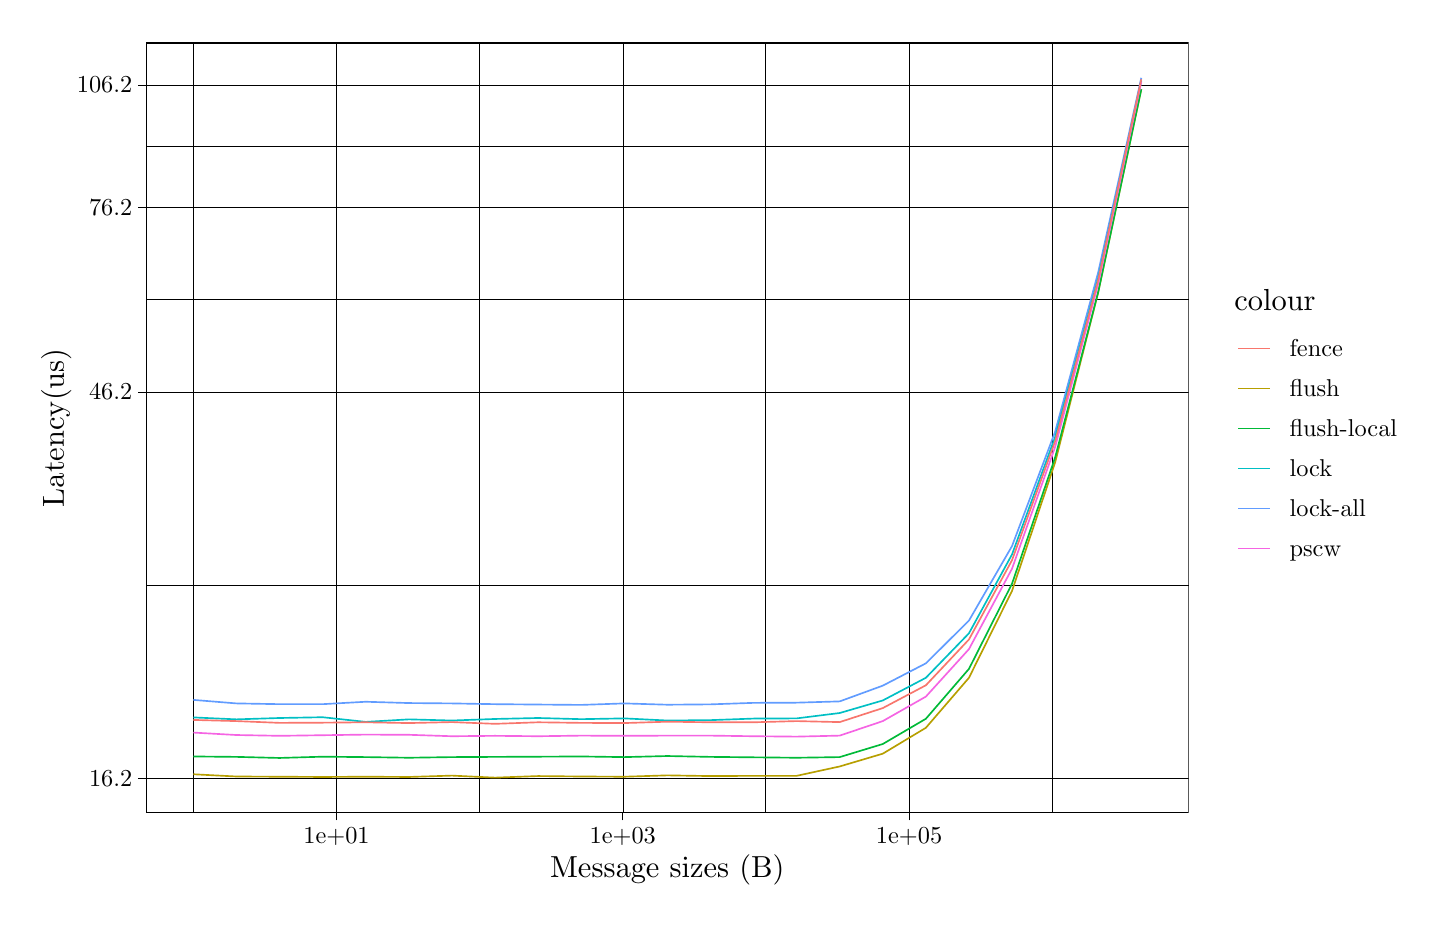
\begin{tikzpicture}[x=1pt,y=1pt]
\definecolor{fillColor}{RGB}{255,255,255}
\path[use as bounding box,fill=fillColor,fill opacity=0.00] (0,0) rectangle (505.89,314.37);
\begin{scope}
\path[clip] (  0.00,  0.00) rectangle (505.89,314.37);
\definecolor{drawColor}{RGB}{255,255,255}
\definecolor{fillColor}{RGB}{255,255,255}

\path[draw=drawColor,line width= 0.6pt,line join=round,line cap=round,fill=fillColor] (  0.00,  0.00) rectangle (505.89,314.37);
\end{scope}
\begin{scope}
\path[clip] ( 42.76, 30.72) rectangle (419.53,308.87);
\definecolor{fillColor}{RGB}{255,255,255}

\path[fill=fillColor] ( 42.76, 30.72) rectangle (419.53,308.87);
\definecolor{drawColor}{RGB}{0,0,0}

\path[draw=drawColor,line width= 0.0pt,line join=round] ( 42.76,112.88) --
	(419.53,112.88);

\path[draw=drawColor,line width= 0.0pt,line join=round] ( 42.76,216.06) --
	(419.53,216.06);

\path[draw=drawColor,line width= 0.0pt,line join=round] ( 42.76,271.52) --
	(419.53,271.52);

\path[draw=drawColor,line width= 0.0pt,line join=round] ( 59.89, 30.72) --
	( 59.89,308.87);

\path[draw=drawColor,line width= 0.0pt,line join=round] (163.32, 30.72) --
	(163.32,308.87);

\path[draw=drawColor,line width= 0.0pt,line join=round] (266.76, 30.72) --
	(266.76,308.87);

\path[draw=drawColor,line width= 0.0pt,line join=round] (370.20, 30.72) --
	(370.20,308.87);

\path[draw=drawColor,line width= 0.1pt,line join=round] ( 42.76, 43.04) --
	(419.53, 43.04);

\path[draw=drawColor,line width= 0.1pt,line join=round] ( 42.76,182.71) --
	(419.53,182.71);

\path[draw=drawColor,line width= 0.1pt,line join=round] ( 42.76,249.40) --
	(419.53,249.40);

\path[draw=drawColor,line width= 0.1pt,line join=round] ( 42.76,293.65) --
	(419.53,293.65);

\path[draw=drawColor,line width= 0.1pt,line join=round] (111.60, 30.72) --
	(111.60,308.87);

\path[draw=drawColor,line width= 0.1pt,line join=round] (215.04, 30.72) --
	(215.04,308.87);

\path[draw=drawColor,line width= 0.1pt,line join=round] (318.48, 30.72) --
	(318.48,308.87);
\definecolor{drawColor}{RGB}{97,156,255}

\path[draw=drawColor,line width= 0.6pt,line join=round] ( 59.89, 71.46) --
	( 75.45, 70.19) --
	( 91.02, 69.92) --
	(106.59, 69.92) --
	(122.16, 70.79) --
	(137.73, 70.32) --
	(153.30, 70.19) --
	(168.87, 69.92) --
	(184.44, 69.78) --
	(200.01, 69.65) --
	(215.58, 70.19) --
	(231.14, 69.72) --
	(246.71, 69.85) --
	(262.28, 70.39) --
	(277.85, 70.46) --
	(293.42, 70.92) --
	(308.99, 76.61) --
	(324.56, 84.67) --
	(340.13,100.12) --
	(355.70,127.06) --
	(371.27,168.38) --
	(386.83,225.96) --
	(402.40,296.23);
\definecolor{drawColor}{RGB}{0,191,196}

\path[draw=drawColor,line width= 0.6pt,line join=round] ( 59.89, 65.13) --
	( 75.45, 64.43) --
	( 91.02, 64.92) --
	(106.59, 65.20) --
	(122.16, 63.51) --
	(137.73, 64.43) --
	(153.30, 64.01) --
	(168.87, 64.57) --
	(184.44, 64.92) --
	(200.01, 64.50) --
	(215.58, 64.78) --
	(231.14, 64.01) --
	(246.71, 64.15) --
	(262.28, 64.71) --
	(277.85, 64.78) --
	(293.42, 66.72) --
	(308.99, 71.26) --
	(324.56, 79.45) --
	(340.13, 95.53) --
	(355.70,124.05) --
	(371.27,166.44) --
	(386.83,223.88) --
	(402.40,295.18);
\definecolor{drawColor}{RGB}{183,159,0}

\path[draw=drawColor,line width= 0.6pt,line join=round] ( 59.89, 44.59) --
	( 75.45, 43.78) --
	( 91.02, 43.70) --
	(106.59, 43.61) --
	(122.16, 43.70) --
	(137.73, 43.61) --
	(153.30, 44.10) --
	(168.87, 43.37) --
	(184.44, 43.94) --
	(200.01, 43.78) --
	(215.58, 43.70) --
	(231.14, 44.19) --
	(246.71, 43.94) --
	(262.28, 44.02) --
	(277.85, 44.02) --
	(293.42, 47.41) --
	(308.99, 52.03) --
	(324.56, 61.38) --
	(340.13, 79.45) --
	(355.70,110.87) --
	(371.27,157.26) --
	(386.83,218.74) --
	(402.40,292.13);
\definecolor{drawColor}{RGB}{0,186,56}

\path[draw=drawColor,line width= 0.6pt,line join=round] ( 59.89, 51.02) --
	( 75.45, 50.87) --
	( 91.02, 50.48) --
	(106.59, 50.94) --
	(122.16, 50.79) --
	(137.73, 50.56) --
	(153.30, 50.79) --
	(168.87, 50.87) --
	(184.44, 50.94) --
	(200.01, 51.02) --
	(215.58, 50.79) --
	(231.14, 51.18) --
	(246.71, 50.87) --
	(262.28, 50.71) --
	(277.85, 50.56) --
	(293.42, 50.79) --
	(308.99, 55.52) --
	(324.56, 64.64) --
	(340.13, 82.67) --
	(355.70,113.47) --
	(371.27,159.07) --
	(386.83,218.81) --
	(402.40,292.11);
\definecolor{drawColor}{RGB}{245,100,227}

\path[draw=drawColor,line width= 0.6pt,line join=round] ( 59.89, 59.65) --
	( 75.45, 58.77) --
	( 91.02, 58.48) --
	(106.59, 58.70) --
	(122.16, 58.92) --
	(137.73, 58.85) --
	(153.30, 58.33) --
	(168.87, 58.48) --
	(184.44, 58.33) --
	(200.01, 58.55) --
	(215.58, 58.48) --
	(231.14, 58.55) --
	(246.71, 58.55) --
	(262.28, 58.33) --
	(277.85, 58.19) --
	(293.42, 58.55) --
	(308.99, 63.80) --
	(324.56, 72.65) --
	(340.13, 89.81) --
	(355.70,118.89) --
	(371.27,162.87) --
	(386.83,221.83) --
	(402.40,294.85);
\definecolor{drawColor}{RGB}{248,118,109}

\path[draw=drawColor,line width= 0.6pt,line join=round] ( 59.89, 64.22) --
	( 75.45, 63.80) --
	( 91.02, 63.16) --
	(106.59, 63.23) --
	(122.16, 63.37) --
	(137.73, 63.09) --
	(153.30, 63.44) --
	(168.87, 62.81) --
	(184.44, 63.37) --
	(200.01, 63.16) --
	(215.58, 63.09) --
	(231.14, 63.58) --
	(246.71, 63.37) --
	(262.28, 63.37) --
	(277.85, 63.80) --
	(293.42, 63.44) --
	(308.99, 68.50) --
	(324.56, 76.74) --
	(340.13, 93.30) --
	(355.70,121.97) --
	(371.27,164.93) --
	(386.83,223.22) --
	(402.40,295.69);
\definecolor{drawColor}{RGB}{0,0,0}

\path[draw=drawColor,line width= 0.6pt,line join=round,line cap=round] ( 42.76, 30.72) rectangle (419.53,308.87);
\end{scope}
\begin{scope}
\path[clip] (  0.00,  0.00) rectangle (505.89,314.37);
\definecolor{drawColor}{RGB}{0,0,0}

\node[text=drawColor,anchor=base west,inner sep=0pt, outer sep=0pt, scale=  0.88] at ( 22.17, 40.22) {16.2};

\node[text=drawColor,anchor=base west,inner sep=0pt, outer sep=0pt, scale=  0.88] at ( 22.17,179.89) {46.2};

\node[text=drawColor,anchor=base west,inner sep=0pt, outer sep=0pt, scale=  0.88] at ( 22.17,246.58) {76.2};

\node[text=drawColor,anchor=base west,inner sep=0pt, outer sep=0pt, scale=  0.88] at ( 17.77,290.82) {106.2};
\end{scope}
\begin{scope}
\path[clip] (  0.00,  0.00) rectangle (505.89,314.37);
\definecolor{drawColor}{RGB}{0,0,0}

\path[draw=drawColor,line width= 0.3pt,line join=round] ( 40.01, 43.04) --
	( 42.76, 43.04);

\path[draw=drawColor,line width= 0.3pt,line join=round] ( 40.01,182.71) --
	( 42.76,182.71);

\path[draw=drawColor,line width= 0.3pt,line join=round] ( 40.01,249.40) --
	( 42.76,249.40);

\path[draw=drawColor,line width= 0.3pt,line join=round] ( 40.01,293.65) --
	( 42.76,293.65);
\end{scope}
\begin{scope}
\path[clip] (  0.00,  0.00) rectangle (505.89,314.37);
\definecolor{drawColor}{RGB}{0,0,0}

\path[draw=drawColor,line width= 0.3pt,line join=round] (111.60, 27.97) --
	(111.60, 30.72);

\path[draw=drawColor,line width= 0.3pt,line join=round] (215.04, 27.97) --
	(215.04, 30.72);

\path[draw=drawColor,line width= 0.3pt,line join=round] (318.48, 27.97) --
	(318.48, 30.72);
\end{scope}
\begin{scope}
\path[clip] (  0.00,  0.00) rectangle (505.89,314.37);
\definecolor{drawColor}{RGB}{0,0,0}

\node[text=drawColor,anchor=base,inner sep=0pt, outer sep=0pt, scale=  0.88] at (111.60, 19.71) {1e+01};

\node[text=drawColor,anchor=base,inner sep=0pt, outer sep=0pt, scale=  0.88] at (215.04, 19.71) {1e+03};

\node[text=drawColor,anchor=base,inner sep=0pt, outer sep=0pt, scale=  0.88] at (318.48, 19.71) {1e+05};
\end{scope}
\begin{scope}
\path[clip] (  0.00,  0.00) rectangle (505.89,314.37);
\definecolor{drawColor}{RGB}{0,0,0}

\node[text=drawColor,anchor=base,inner sep=0pt, outer sep=0pt, scale=  1.10] at (231.14,  7.44) {Message sizes (B)};
\end{scope}
\begin{scope}
\path[clip] (  0.00,  0.00) rectangle (505.89,314.37);
\definecolor{drawColor}{RGB}{0,0,0}

\node[text=drawColor,rotate= 90.00,anchor=base,inner sep=0pt, outer sep=0pt, scale=  1.10] at ( 13.08,169.80) {Latency(us)};
\end{scope}
\begin{scope}
\path[clip] (  0.00,  0.00) rectangle (505.89,314.37);
\definecolor{fillColor}{RGB}{255,255,255}

\path[fill=fillColor] (430.53,113.43) rectangle (500.39,226.17);
\end{scope}
\begin{scope}
\path[clip] (  0.00,  0.00) rectangle (505.89,314.37);
\definecolor{drawColor}{RGB}{0,0,0}

\node[text=drawColor,anchor=base west,inner sep=0pt, outer sep=0pt, scale=  1.10] at (436.03,212.12) {colour};
\end{scope}
\begin{scope}
\path[clip] (  0.00,  0.00) rectangle (505.89,314.37);
\definecolor{fillColor}{RGB}{255,255,255}

\path[fill=fillColor] (436.03,191.20) rectangle (450.48,205.65);
\end{scope}
\begin{scope}
\path[clip] (  0.00,  0.00) rectangle (505.89,314.37);
\definecolor{drawColor}{RGB}{248,118,109}

\path[draw=drawColor,line width= 0.6pt,line join=round] (437.48,198.42) -- (449.04,198.42);
\end{scope}
\begin{scope}
\path[clip] (  0.00,  0.00) rectangle (505.89,314.37);
\definecolor{drawColor}{RGB}{248,118,109}

\path[draw=drawColor,line width= 0.6pt,line join=round] (437.48,198.42) -- (449.04,198.42);
\end{scope}
\begin{scope}
\path[clip] (  0.00,  0.00) rectangle (505.89,314.37);
\definecolor{drawColor}{RGB}{248,118,109}

\path[draw=drawColor,line width= 0.6pt,line join=round] (437.48,198.42) -- (449.04,198.42);
\end{scope}
\begin{scope}
\path[clip] (  0.00,  0.00) rectangle (505.89,314.37);
\definecolor{drawColor}{RGB}{248,118,109}

\path[draw=drawColor,line width= 0.6pt,line join=round] (437.48,198.42) -- (449.04,198.42);
\end{scope}
\begin{scope}
\path[clip] (  0.00,  0.00) rectangle (505.89,314.37);
\definecolor{drawColor}{RGB}{248,118,109}

\path[draw=drawColor,line width= 0.6pt,line join=round] (437.48,198.42) -- (449.04,198.42);
\end{scope}
\begin{scope}
\path[clip] (  0.00,  0.00) rectangle (505.89,314.37);
\definecolor{drawColor}{RGB}{248,118,109}

\path[draw=drawColor,line width= 0.6pt,line join=round] (437.48,198.42) -- (449.04,198.42);
\end{scope}
\begin{scope}
\path[clip] (  0.00,  0.00) rectangle (505.89,314.37);
\definecolor{fillColor}{RGB}{255,255,255}

\path[fill=fillColor] (436.03,176.74) rectangle (450.48,191.20);
\end{scope}
\begin{scope}
\path[clip] (  0.00,  0.00) rectangle (505.89,314.37);
\definecolor{drawColor}{RGB}{183,159,0}

\path[draw=drawColor,line width= 0.6pt,line join=round] (437.48,183.97) -- (449.04,183.97);
\end{scope}
\begin{scope}
\path[clip] (  0.00,  0.00) rectangle (505.89,314.37);
\definecolor{drawColor}{RGB}{183,159,0}

\path[draw=drawColor,line width= 0.6pt,line join=round] (437.48,183.97) -- (449.04,183.97);
\end{scope}
\begin{scope}
\path[clip] (  0.00,  0.00) rectangle (505.89,314.37);
\definecolor{drawColor}{RGB}{183,159,0}

\path[draw=drawColor,line width= 0.6pt,line join=round] (437.48,183.97) -- (449.04,183.97);
\end{scope}
\begin{scope}
\path[clip] (  0.00,  0.00) rectangle (505.89,314.37);
\definecolor{drawColor}{RGB}{183,159,0}

\path[draw=drawColor,line width= 0.6pt,line join=round] (437.48,183.97) -- (449.04,183.97);
\end{scope}
\begin{scope}
\path[clip] (  0.00,  0.00) rectangle (505.89,314.37);
\definecolor{drawColor}{RGB}{183,159,0}

\path[draw=drawColor,line width= 0.6pt,line join=round] (437.48,183.97) -- (449.04,183.97);
\end{scope}
\begin{scope}
\path[clip] (  0.00,  0.00) rectangle (505.89,314.37);
\definecolor{drawColor}{RGB}{183,159,0}

\path[draw=drawColor,line width= 0.6pt,line join=round] (437.48,183.97) -- (449.04,183.97);
\end{scope}
\begin{scope}
\path[clip] (  0.00,  0.00) rectangle (505.89,314.37);
\definecolor{fillColor}{RGB}{255,255,255}

\path[fill=fillColor] (436.03,162.29) rectangle (450.48,176.74);
\end{scope}
\begin{scope}
\path[clip] (  0.00,  0.00) rectangle (505.89,314.37);
\definecolor{drawColor}{RGB}{0,186,56}

\path[draw=drawColor,line width= 0.6pt,line join=round] (437.48,169.52) -- (449.04,169.52);
\end{scope}
\begin{scope}
\path[clip] (  0.00,  0.00) rectangle (505.89,314.37);
\definecolor{drawColor}{RGB}{0,186,56}

\path[draw=drawColor,line width= 0.6pt,line join=round] (437.48,169.52) -- (449.04,169.52);
\end{scope}
\begin{scope}
\path[clip] (  0.00,  0.00) rectangle (505.89,314.37);
\definecolor{drawColor}{RGB}{0,186,56}

\path[draw=drawColor,line width= 0.6pt,line join=round] (437.48,169.52) -- (449.04,169.52);
\end{scope}
\begin{scope}
\path[clip] (  0.00,  0.00) rectangle (505.89,314.37);
\definecolor{drawColor}{RGB}{0,186,56}

\path[draw=drawColor,line width= 0.6pt,line join=round] (437.48,169.52) -- (449.04,169.52);
\end{scope}
\begin{scope}
\path[clip] (  0.00,  0.00) rectangle (505.89,314.37);
\definecolor{drawColor}{RGB}{0,186,56}

\path[draw=drawColor,line width= 0.6pt,line join=round] (437.48,169.52) -- (449.04,169.52);
\end{scope}
\begin{scope}
\path[clip] (  0.00,  0.00) rectangle (505.89,314.37);
\definecolor{drawColor}{RGB}{0,186,56}

\path[draw=drawColor,line width= 0.6pt,line join=round] (437.48,169.52) -- (449.04,169.52);
\end{scope}
\begin{scope}
\path[clip] (  0.00,  0.00) rectangle (505.89,314.37);
\definecolor{fillColor}{RGB}{255,255,255}

\path[fill=fillColor] (436.03,147.84) rectangle (450.48,162.29);
\end{scope}
\begin{scope}
\path[clip] (  0.00,  0.00) rectangle (505.89,314.37);
\definecolor{drawColor}{RGB}{0,191,196}

\path[draw=drawColor,line width= 0.6pt,line join=round] (437.48,155.06) -- (449.04,155.06);
\end{scope}
\begin{scope}
\path[clip] (  0.00,  0.00) rectangle (505.89,314.37);
\definecolor{drawColor}{RGB}{0,191,196}

\path[draw=drawColor,line width= 0.6pt,line join=round] (437.48,155.06) -- (449.04,155.06);
\end{scope}
\begin{scope}
\path[clip] (  0.00,  0.00) rectangle (505.89,314.37);
\definecolor{drawColor}{RGB}{0,191,196}

\path[draw=drawColor,line width= 0.6pt,line join=round] (437.48,155.06) -- (449.04,155.06);
\end{scope}
\begin{scope}
\path[clip] (  0.00,  0.00) rectangle (505.89,314.37);
\definecolor{drawColor}{RGB}{0,191,196}

\path[draw=drawColor,line width= 0.6pt,line join=round] (437.48,155.06) -- (449.04,155.06);
\end{scope}
\begin{scope}
\path[clip] (  0.00,  0.00) rectangle (505.89,314.37);
\definecolor{drawColor}{RGB}{0,191,196}

\path[draw=drawColor,line width= 0.6pt,line join=round] (437.48,155.06) -- (449.04,155.06);
\end{scope}
\begin{scope}
\path[clip] (  0.00,  0.00) rectangle (505.89,314.37);
\definecolor{drawColor}{RGB}{0,191,196}

\path[draw=drawColor,line width= 0.6pt,line join=round] (437.48,155.06) -- (449.04,155.06);
\end{scope}
\begin{scope}
\path[clip] (  0.00,  0.00) rectangle (505.89,314.37);
\definecolor{fillColor}{RGB}{255,255,255}

\path[fill=fillColor] (436.03,133.38) rectangle (450.48,147.84);
\end{scope}
\begin{scope}
\path[clip] (  0.00,  0.00) rectangle (505.89,314.37);
\definecolor{drawColor}{RGB}{97,156,255}

\path[draw=drawColor,line width= 0.6pt,line join=round] (437.48,140.61) -- (449.04,140.61);
\end{scope}
\begin{scope}
\path[clip] (  0.00,  0.00) rectangle (505.89,314.37);
\definecolor{drawColor}{RGB}{97,156,255}

\path[draw=drawColor,line width= 0.6pt,line join=round] (437.48,140.61) -- (449.04,140.61);
\end{scope}
\begin{scope}
\path[clip] (  0.00,  0.00) rectangle (505.89,314.37);
\definecolor{drawColor}{RGB}{97,156,255}

\path[draw=drawColor,line width= 0.6pt,line join=round] (437.48,140.61) -- (449.04,140.61);
\end{scope}
\begin{scope}
\path[clip] (  0.00,  0.00) rectangle (505.89,314.37);
\definecolor{drawColor}{RGB}{97,156,255}

\path[draw=drawColor,line width= 0.6pt,line join=round] (437.48,140.61) -- (449.04,140.61);
\end{scope}
\begin{scope}
\path[clip] (  0.00,  0.00) rectangle (505.89,314.37);
\definecolor{drawColor}{RGB}{97,156,255}

\path[draw=drawColor,line width= 0.6pt,line join=round] (437.48,140.61) -- (449.04,140.61);
\end{scope}
\begin{scope}
\path[clip] (  0.00,  0.00) rectangle (505.89,314.37);
\definecolor{drawColor}{RGB}{97,156,255}

\path[draw=drawColor,line width= 0.6pt,line join=round] (437.48,140.61) -- (449.04,140.61);
\end{scope}
\begin{scope}
\path[clip] (  0.00,  0.00) rectangle (505.89,314.37);
\definecolor{fillColor}{RGB}{255,255,255}

\path[fill=fillColor] (436.03,118.93) rectangle (450.48,133.38);
\end{scope}
\begin{scope}
\path[clip] (  0.00,  0.00) rectangle (505.89,314.37);
\definecolor{drawColor}{RGB}{245,100,227}

\path[draw=drawColor,line width= 0.6pt,line join=round] (437.48,126.15) -- (449.04,126.15);
\end{scope}
\begin{scope}
\path[clip] (  0.00,  0.00) rectangle (505.89,314.37);
\definecolor{drawColor}{RGB}{245,100,227}

\path[draw=drawColor,line width= 0.6pt,line join=round] (437.48,126.15) -- (449.04,126.15);
\end{scope}
\begin{scope}
\path[clip] (  0.00,  0.00) rectangle (505.89,314.37);
\definecolor{drawColor}{RGB}{245,100,227}

\path[draw=drawColor,line width= 0.6pt,line join=round] (437.48,126.15) -- (449.04,126.15);
\end{scope}
\begin{scope}
\path[clip] (  0.00,  0.00) rectangle (505.89,314.37);
\definecolor{drawColor}{RGB}{245,100,227}

\path[draw=drawColor,line width= 0.6pt,line join=round] (437.48,126.15) -- (449.04,126.15);
\end{scope}
\begin{scope}
\path[clip] (  0.00,  0.00) rectangle (505.89,314.37);
\definecolor{drawColor}{RGB}{245,100,227}

\path[draw=drawColor,line width= 0.6pt,line join=round] (437.48,126.15) -- (449.04,126.15);
\end{scope}
\begin{scope}
\path[clip] (  0.00,  0.00) rectangle (505.89,314.37);
\definecolor{drawColor}{RGB}{245,100,227}

\path[draw=drawColor,line width= 0.6pt,line join=round] (437.48,126.15) -- (449.04,126.15);
\end{scope}
\begin{scope}
\path[clip] (  0.00,  0.00) rectangle (505.89,314.37);
\definecolor{drawColor}{RGB}{0,0,0}

\node[text=drawColor,anchor=base west,inner sep=0pt, outer sep=0pt, scale=  0.88] at (455.98,195.39) {fence};
\end{scope}
\begin{scope}
\path[clip] (  0.00,  0.00) rectangle (505.89,314.37);
\definecolor{drawColor}{RGB}{0,0,0}

\node[text=drawColor,anchor=base west,inner sep=0pt, outer sep=0pt, scale=  0.88] at (455.98,180.94) {flush};
\end{scope}
\begin{scope}
\path[clip] (  0.00,  0.00) rectangle (505.89,314.37);
\definecolor{drawColor}{RGB}{0,0,0}

\node[text=drawColor,anchor=base west,inner sep=0pt, outer sep=0pt, scale=  0.88] at (455.98,166.49) {flush-local};
\end{scope}
\begin{scope}
\path[clip] (  0.00,  0.00) rectangle (505.89,314.37);
\definecolor{drawColor}{RGB}{0,0,0}

\node[text=drawColor,anchor=base west,inner sep=0pt, outer sep=0pt, scale=  0.88] at (455.98,152.03) {lock};
\end{scope}
\begin{scope}
\path[clip] (  0.00,  0.00) rectangle (505.89,314.37);
\definecolor{drawColor}{RGB}{0,0,0}

\node[text=drawColor,anchor=base west,inner sep=0pt, outer sep=0pt, scale=  0.88] at (455.98,137.58) {lock-all};
\end{scope}
\begin{scope}
\path[clip] (  0.00,  0.00) rectangle (505.89,314.37);
\definecolor{drawColor}{RGB}{0,0,0}

\node[text=drawColor,anchor=base west,inner sep=0pt, outer sep=0pt, scale=  0.88] at (455.98,123.12) {pscw};
\end{scope}
\end{tikzpicture}

	\caption{1 node, get latency, gpu-gpu, window create, sync algorithm comparisons}
\end{figure}

\begin{figure}
	% Created by tikzDevice version 0.10.1 on 2020-02-15 15:54:51
% !TEX encoding = UTF-8 Unicode
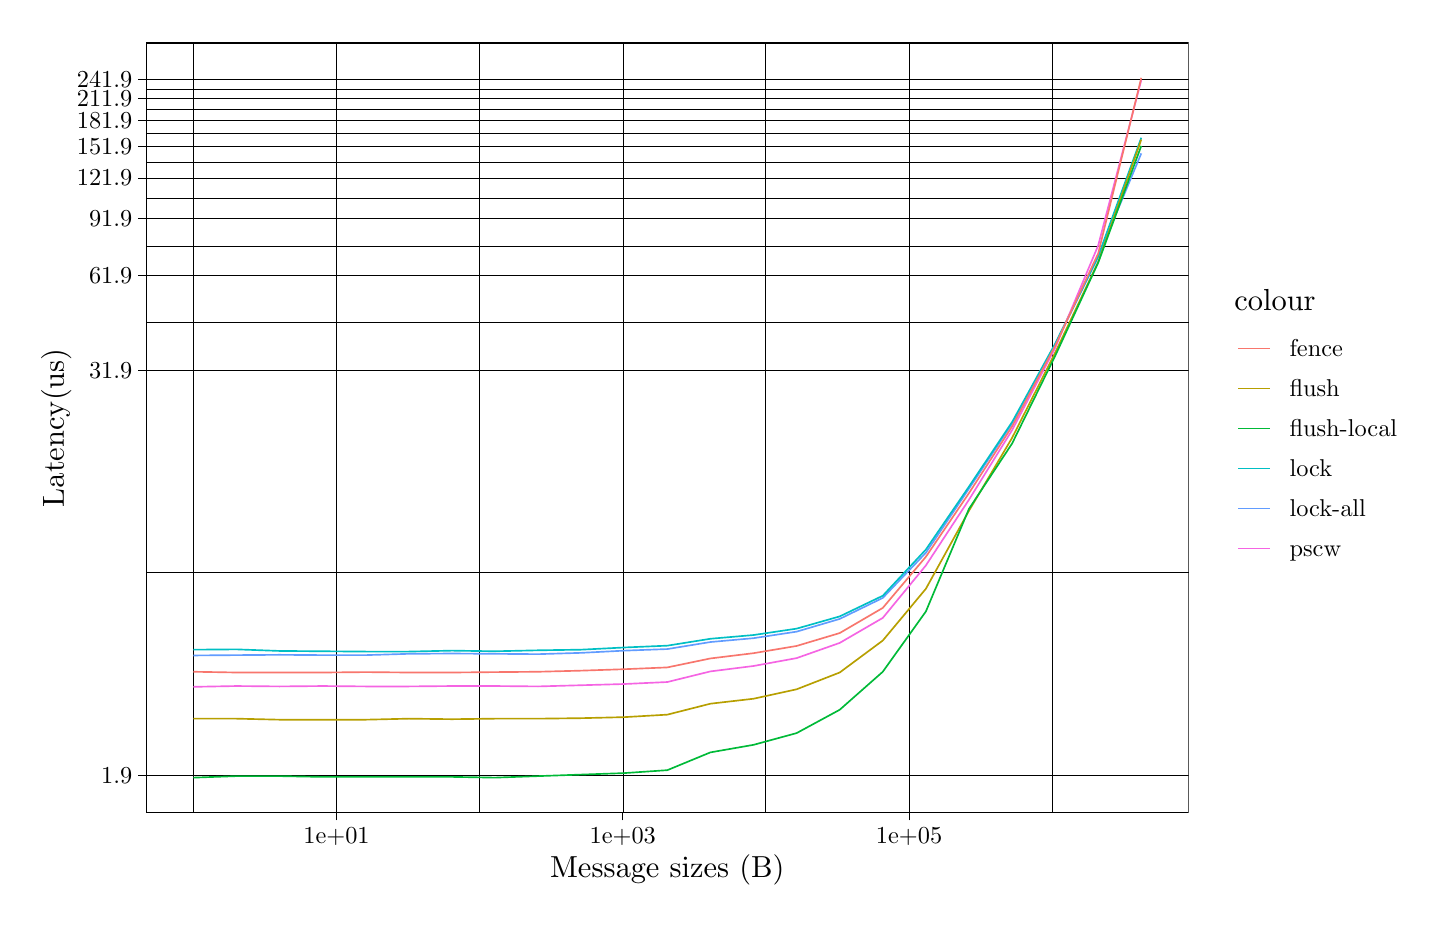
\begin{tikzpicture}[x=1pt,y=1pt]
\definecolor{fillColor}{RGB}{255,255,255}
\path[use as bounding box,fill=fillColor,fill opacity=0.00] (0,0) rectangle (505.89,314.37);
\begin{scope}
\path[clip] (  0.00,  0.00) rectangle (505.89,314.37);
\definecolor{drawColor}{RGB}{255,255,255}
\definecolor{fillColor}{RGB}{255,255,255}

\path[draw=drawColor,line width= 0.6pt,line join=round,line cap=round,fill=fillColor] (  0.00,  0.00) rectangle (505.89,314.37);
\end{scope}
\begin{scope}
\path[clip] ( 42.76, 30.72) rectangle (419.53,308.87);
\definecolor{fillColor}{RGB}{255,255,255}

\path[fill=fillColor] ( 42.76, 30.72) rectangle (419.53,308.87);
\definecolor{drawColor}{RGB}{0,0,0}

\path[draw=drawColor,line width= 0.0pt,line join=round] ( 42.76,117.35) --
	(419.53,117.35);

\path[draw=drawColor,line width= 0.0pt,line join=round] ( 42.76,207.71) --
	(419.53,207.71);

\path[draw=drawColor,line width= 0.0pt,line join=round] ( 42.76,235.15) --
	(419.53,235.15);

\path[draw=drawColor,line width= 0.0pt,line join=round] ( 42.76,252.72) --
	(419.53,252.72);

\path[draw=drawColor,line width= 0.0pt,line join=round] ( 42.76,265.76) --
	(419.53,265.76);

\path[draw=drawColor,line width= 0.0pt,line join=round] ( 42.76,276.14) --
	(419.53,276.14);

\path[draw=drawColor,line width= 0.0pt,line join=round] ( 42.76,284.77) --
	(419.53,284.77);

\path[draw=drawColor,line width= 0.0pt,line join=round] ( 42.76,292.17) --
	(419.53,292.17);

\path[draw=drawColor,line width= 0.0pt,line join=round] ( 59.89, 30.72) --
	( 59.89,308.87);

\path[draw=drawColor,line width= 0.0pt,line join=round] (163.32, 30.72) --
	(163.32,308.87);

\path[draw=drawColor,line width= 0.0pt,line join=round] (266.76, 30.72) --
	(266.76,308.87);

\path[draw=drawColor,line width= 0.0pt,line join=round] (370.20, 30.72) --
	(370.20,308.87);

\path[draw=drawColor,line width= 0.1pt,line join=round] ( 42.76, 44.19) --
	(419.53, 44.19);

\path[draw=drawColor,line width= 0.1pt,line join=round] ( 42.76,190.51) --
	(419.53,190.51);

\path[draw=drawColor,line width= 0.1pt,line join=round] ( 42.76,224.90) --
	(419.53,224.90);

\path[draw=drawColor,line width= 0.1pt,line join=round] ( 42.76,245.40) --
	(419.53,245.40);

\path[draw=drawColor,line width= 0.1pt,line join=round] ( 42.76,260.05) --
	(419.53,260.05);

\path[draw=drawColor,line width= 0.1pt,line join=round] ( 42.76,271.46) --
	(419.53,271.46);

\path[draw=drawColor,line width= 0.1pt,line join=round] ( 42.76,280.81) --
	(419.53,280.81);

\path[draw=drawColor,line width= 0.1pt,line join=round] ( 42.76,288.73) --
	(419.53,288.73);

\path[draw=drawColor,line width= 0.1pt,line join=round] ( 42.76,295.60) --
	(419.53,295.60);

\path[draw=drawColor,line width= 0.1pt,line join=round] (111.60, 30.72) --
	(111.60,308.87);

\path[draw=drawColor,line width= 0.1pt,line join=round] (215.04, 30.72) --
	(215.04,308.87);

\path[draw=drawColor,line width= 0.1pt,line join=round] (318.48, 30.72) --
	(318.48,308.87);
\definecolor{drawColor}{RGB}{97,156,255}

\path[draw=drawColor,line width= 0.6pt,line join=round] ( 59.89, 87.52) --
	( 75.45, 87.64) --
	( 91.02, 87.75) --
	(106.59, 87.64) --
	(122.16, 87.64) --
	(137.73, 88.11) --
	(153.30, 88.22) --
	(168.87, 88.11) --
	(184.44, 87.99) --
	(200.01, 88.46) --
	(215.58, 89.26) --
	(231.14, 89.83) --
	(246.71, 92.37) --
	(262.28, 93.76) --
	(277.85, 96.12) --
	(293.42,100.72) --
	(308.99,108.31) --
	(324.56,124.64) --
	(340.13,147.79) --
	(355.70,171.26) --
	(371.27,199.78) --
	(386.83,231.54) --
	(402.40,268.94);
\definecolor{drawColor}{RGB}{0,191,196}

\path[draw=drawColor,line width= 0.6pt,line join=round] ( 59.89, 89.61) --
	( 75.45, 89.72) --
	( 91.02, 89.15) --
	(106.59, 89.03) --
	(122.16, 88.92) --
	(137.73, 88.92) --
	(153.30, 89.26) --
	(168.87, 89.03) --
	(184.44, 89.38) --
	(200.01, 89.61) --
	(215.58, 90.40) --
	(231.14, 91.06) --
	(246.71, 93.55) --
	(262.28, 94.90) --
	(277.85, 97.21) --
	(293.42,101.63) --
	(308.99,109.10) --
	(324.56,125.79) --
	(340.13,148.53) --
	(355.70,171.82) --
	(371.27,200.17) --
	(386.83,231.76) --
	(402.40,274.59);
\definecolor{drawColor}{RGB}{183,159,0}

\path[draw=drawColor,line width= 0.6pt,line join=round] ( 59.89, 64.68) --
	( 75.45, 64.68) --
	( 91.02, 64.31) --
	(106.59, 64.31) --
	(122.16, 64.31) --
	(137.73, 64.68) --
	(153.30, 64.49) --
	(168.87, 64.68) --
	(184.44, 64.68) --
	(200.01, 64.86) --
	(215.58, 65.23) --
	(231.14, 66.13) --
	(246.71, 70.09) --
	(262.28, 71.88) --
	(277.85, 75.29) --
	(293.42, 81.36) --
	(308.99, 92.91) --
	(324.56,111.61) --
	(340.13,139.80) --
	(355.70,166.11) --
	(371.27,196.88) --
	(386.83,229.73) --
	(402.40,273.94);
\definecolor{drawColor}{RGB}{0,186,56}

\path[draw=drawColor,line width= 0.6pt,line join=round] ( 59.89, 43.37) --
	( 75.45, 43.92) --
	( 91.02, 43.92) --
	(106.59, 43.64) --
	(122.16, 43.64) --
	(137.73, 43.64) --
	(153.30, 43.64) --
	(168.87, 43.37) --
	(184.44, 43.92) --
	(200.01, 44.47) --
	(215.58, 45.01) --
	(231.14, 46.07) --
	(246.71, 52.50) --
	(262.28, 55.22) --
	(277.85, 59.46) --
	(293.42, 67.89) --
	(308.99, 81.63) --
	(324.56,103.41) --
	(340.13,140.48) --
	(355.70,164.07) --
	(371.27,195.74) --
	(386.83,229.45) --
	(402.40,271.66);
\definecolor{drawColor}{RGB}{245,100,227}

\path[draw=drawColor,line width= 0.6pt,line join=round] ( 59.89, 76.18) --
	( 75.45, 76.47) --
	( 91.02, 76.33) --
	(106.59, 76.47) --
	(122.16, 76.33) --
	(137.73, 76.33) --
	(153.30, 76.47) --
	(168.87, 76.47) --
	(184.44, 76.33) --
	(200.01, 76.76) --
	(215.58, 77.20) --
	(231.14, 77.92) --
	(246.71, 81.76) --
	(262.28, 83.71) --
	(277.85, 86.56) --
	(293.42, 92.05) --
	(308.99,101.09) --
	(324.56,120.04) --
	(340.13,143.79) --
	(355.70,168.90) --
	(371.27,198.62) --
	(386.83,235.67) --
	(402.40,295.41);
\definecolor{drawColor}{RGB}{248,118,109}

\path[draw=drawColor,line width= 0.6pt,line join=round] ( 59.89, 81.63) --
	( 75.45, 81.36) --
	( 91.02, 81.36) --
	(106.59, 81.36) --
	(122.16, 81.50) --
	(137.73, 81.36) --
	(153.30, 81.36) --
	(168.87, 81.50) --
	(184.44, 81.63) --
	(200.01, 82.03) --
	(215.58, 82.55) --
	(231.14, 83.20) --
	(246.71, 86.44) --
	(262.28, 88.34) --
	(277.85, 90.95) --
	(293.42, 95.61) --
	(308.99,104.70) --
	(324.56,123.17) --
	(340.13,146.17) --
	(355.70,170.26) --
	(371.27,199.38) --
	(386.83,232.79) --
	(402.40,296.23);
\definecolor{drawColor}{RGB}{0,0,0}

\path[draw=drawColor,line width= 0.6pt,line join=round,line cap=round] ( 42.76, 30.72) rectangle (419.53,308.87);
\end{scope}
\begin{scope}
\path[clip] (  0.00,  0.00) rectangle (505.89,314.37);
\definecolor{drawColor}{RGB}{0,0,0}

\node[text=drawColor,anchor=base west,inner sep=0pt, outer sep=0pt, scale=  0.88] at ( 26.57, 41.37) {1.9};

\node[text=drawColor,anchor=base west,inner sep=0pt, outer sep=0pt, scale=  0.88] at ( 22.17,187.69) {31.9};

\node[text=drawColor,anchor=base west,inner sep=0pt, outer sep=0pt, scale=  0.88] at ( 22.17,222.08) {61.9};

\node[text=drawColor,anchor=base west,inner sep=0pt, outer sep=0pt, scale=  0.88] at ( 22.17,242.57) {91.9};

\node[text=drawColor,anchor=base west,inner sep=0pt, outer sep=0pt, scale=  0.88] at ( 17.77,257.23) {121.9};

\node[text=drawColor,anchor=base west,inner sep=0pt, outer sep=0pt, scale=  0.88] at ( 17.77,268.64) {151.9};

\node[text=drawColor,anchor=base west,inner sep=0pt, outer sep=0pt, scale=  0.88] at ( 17.77,277.99) {181.9};

\node[text=drawColor,anchor=base west,inner sep=0pt, outer sep=0pt, scale=  0.88] at ( 17.77,285.91) {211.9};

\node[text=drawColor,anchor=base west,inner sep=0pt, outer sep=0pt, scale=  0.88] at ( 17.77,292.78) {241.9};
\end{scope}
\begin{scope}
\path[clip] (  0.00,  0.00) rectangle (505.89,314.37);
\definecolor{drawColor}{RGB}{0,0,0}

\path[draw=drawColor,line width= 0.3pt,line join=round] ( 40.01, 44.19) --
	( 42.76, 44.19);

\path[draw=drawColor,line width= 0.3pt,line join=round] ( 40.01,190.51) --
	( 42.76,190.51);

\path[draw=drawColor,line width= 0.3pt,line join=round] ( 40.01,224.90) --
	( 42.76,224.90);

\path[draw=drawColor,line width= 0.3pt,line join=round] ( 40.01,245.40) --
	( 42.76,245.40);

\path[draw=drawColor,line width= 0.3pt,line join=round] ( 40.01,260.05) --
	( 42.76,260.05);

\path[draw=drawColor,line width= 0.3pt,line join=round] ( 40.01,271.46) --
	( 42.76,271.46);

\path[draw=drawColor,line width= 0.3pt,line join=round] ( 40.01,280.81) --
	( 42.76,280.81);

\path[draw=drawColor,line width= 0.3pt,line join=round] ( 40.01,288.73) --
	( 42.76,288.73);

\path[draw=drawColor,line width= 0.3pt,line join=round] ( 40.01,295.60) --
	( 42.76,295.60);
\end{scope}
\begin{scope}
\path[clip] (  0.00,  0.00) rectangle (505.89,314.37);
\definecolor{drawColor}{RGB}{0,0,0}

\path[draw=drawColor,line width= 0.3pt,line join=round] (111.60, 27.97) --
	(111.60, 30.72);

\path[draw=drawColor,line width= 0.3pt,line join=round] (215.04, 27.97) --
	(215.04, 30.72);

\path[draw=drawColor,line width= 0.3pt,line join=round] (318.48, 27.97) --
	(318.48, 30.72);
\end{scope}
\begin{scope}
\path[clip] (  0.00,  0.00) rectangle (505.89,314.37);
\definecolor{drawColor}{RGB}{0,0,0}

\node[text=drawColor,anchor=base,inner sep=0pt, outer sep=0pt, scale=  0.88] at (111.60, 19.71) {1e+01};

\node[text=drawColor,anchor=base,inner sep=0pt, outer sep=0pt, scale=  0.88] at (215.04, 19.71) {1e+03};

\node[text=drawColor,anchor=base,inner sep=0pt, outer sep=0pt, scale=  0.88] at (318.48, 19.71) {1e+05};
\end{scope}
\begin{scope}
\path[clip] (  0.00,  0.00) rectangle (505.89,314.37);
\definecolor{drawColor}{RGB}{0,0,0}

\node[text=drawColor,anchor=base,inner sep=0pt, outer sep=0pt, scale=  1.10] at (231.14,  7.44) {Message sizes (B)};
\end{scope}
\begin{scope}
\path[clip] (  0.00,  0.00) rectangle (505.89,314.37);
\definecolor{drawColor}{RGB}{0,0,0}

\node[text=drawColor,rotate= 90.00,anchor=base,inner sep=0pt, outer sep=0pt, scale=  1.10] at ( 13.08,169.80) {Latency(us)};
\end{scope}
\begin{scope}
\path[clip] (  0.00,  0.00) rectangle (505.89,314.37);
\definecolor{fillColor}{RGB}{255,255,255}

\path[fill=fillColor] (430.53,113.43) rectangle (500.39,226.17);
\end{scope}
\begin{scope}
\path[clip] (  0.00,  0.00) rectangle (505.89,314.37);
\definecolor{drawColor}{RGB}{0,0,0}

\node[text=drawColor,anchor=base west,inner sep=0pt, outer sep=0pt, scale=  1.10] at (436.03,212.12) {colour};
\end{scope}
\begin{scope}
\path[clip] (  0.00,  0.00) rectangle (505.89,314.37);
\definecolor{fillColor}{RGB}{255,255,255}

\path[fill=fillColor] (436.03,191.20) rectangle (450.48,205.65);
\end{scope}
\begin{scope}
\path[clip] (  0.00,  0.00) rectangle (505.89,314.37);
\definecolor{drawColor}{RGB}{248,118,109}

\path[draw=drawColor,line width= 0.6pt,line join=round] (437.48,198.42) -- (449.04,198.42);
\end{scope}
\begin{scope}
\path[clip] (  0.00,  0.00) rectangle (505.89,314.37);
\definecolor{drawColor}{RGB}{248,118,109}

\path[draw=drawColor,line width= 0.6pt,line join=round] (437.48,198.42) -- (449.04,198.42);
\end{scope}
\begin{scope}
\path[clip] (  0.00,  0.00) rectangle (505.89,314.37);
\definecolor{drawColor}{RGB}{248,118,109}

\path[draw=drawColor,line width= 0.6pt,line join=round] (437.48,198.42) -- (449.04,198.42);
\end{scope}
\begin{scope}
\path[clip] (  0.00,  0.00) rectangle (505.89,314.37);
\definecolor{drawColor}{RGB}{248,118,109}

\path[draw=drawColor,line width= 0.6pt,line join=round] (437.48,198.42) -- (449.04,198.42);
\end{scope}
\begin{scope}
\path[clip] (  0.00,  0.00) rectangle (505.89,314.37);
\definecolor{drawColor}{RGB}{248,118,109}

\path[draw=drawColor,line width= 0.6pt,line join=round] (437.48,198.42) -- (449.04,198.42);
\end{scope}
\begin{scope}
\path[clip] (  0.00,  0.00) rectangle (505.89,314.37);
\definecolor{drawColor}{RGB}{248,118,109}

\path[draw=drawColor,line width= 0.6pt,line join=round] (437.48,198.42) -- (449.04,198.42);
\end{scope}
\begin{scope}
\path[clip] (  0.00,  0.00) rectangle (505.89,314.37);
\definecolor{fillColor}{RGB}{255,255,255}

\path[fill=fillColor] (436.03,176.74) rectangle (450.48,191.20);
\end{scope}
\begin{scope}
\path[clip] (  0.00,  0.00) rectangle (505.89,314.37);
\definecolor{drawColor}{RGB}{183,159,0}

\path[draw=drawColor,line width= 0.6pt,line join=round] (437.48,183.97) -- (449.04,183.97);
\end{scope}
\begin{scope}
\path[clip] (  0.00,  0.00) rectangle (505.89,314.37);
\definecolor{drawColor}{RGB}{183,159,0}

\path[draw=drawColor,line width= 0.6pt,line join=round] (437.48,183.97) -- (449.04,183.97);
\end{scope}
\begin{scope}
\path[clip] (  0.00,  0.00) rectangle (505.89,314.37);
\definecolor{drawColor}{RGB}{183,159,0}

\path[draw=drawColor,line width= 0.6pt,line join=round] (437.48,183.97) -- (449.04,183.97);
\end{scope}
\begin{scope}
\path[clip] (  0.00,  0.00) rectangle (505.89,314.37);
\definecolor{drawColor}{RGB}{183,159,0}

\path[draw=drawColor,line width= 0.6pt,line join=round] (437.48,183.97) -- (449.04,183.97);
\end{scope}
\begin{scope}
\path[clip] (  0.00,  0.00) rectangle (505.89,314.37);
\definecolor{drawColor}{RGB}{183,159,0}

\path[draw=drawColor,line width= 0.6pt,line join=round] (437.48,183.97) -- (449.04,183.97);
\end{scope}
\begin{scope}
\path[clip] (  0.00,  0.00) rectangle (505.89,314.37);
\definecolor{drawColor}{RGB}{183,159,0}

\path[draw=drawColor,line width= 0.6pt,line join=round] (437.48,183.97) -- (449.04,183.97);
\end{scope}
\begin{scope}
\path[clip] (  0.00,  0.00) rectangle (505.89,314.37);
\definecolor{fillColor}{RGB}{255,255,255}

\path[fill=fillColor] (436.03,162.29) rectangle (450.48,176.74);
\end{scope}
\begin{scope}
\path[clip] (  0.00,  0.00) rectangle (505.89,314.37);
\definecolor{drawColor}{RGB}{0,186,56}

\path[draw=drawColor,line width= 0.6pt,line join=round] (437.48,169.52) -- (449.04,169.52);
\end{scope}
\begin{scope}
\path[clip] (  0.00,  0.00) rectangle (505.89,314.37);
\definecolor{drawColor}{RGB}{0,186,56}

\path[draw=drawColor,line width= 0.6pt,line join=round] (437.48,169.52) -- (449.04,169.52);
\end{scope}
\begin{scope}
\path[clip] (  0.00,  0.00) rectangle (505.89,314.37);
\definecolor{drawColor}{RGB}{0,186,56}

\path[draw=drawColor,line width= 0.6pt,line join=round] (437.48,169.52) -- (449.04,169.52);
\end{scope}
\begin{scope}
\path[clip] (  0.00,  0.00) rectangle (505.89,314.37);
\definecolor{drawColor}{RGB}{0,186,56}

\path[draw=drawColor,line width= 0.6pt,line join=round] (437.48,169.52) -- (449.04,169.52);
\end{scope}
\begin{scope}
\path[clip] (  0.00,  0.00) rectangle (505.89,314.37);
\definecolor{drawColor}{RGB}{0,186,56}

\path[draw=drawColor,line width= 0.6pt,line join=round] (437.48,169.52) -- (449.04,169.52);
\end{scope}
\begin{scope}
\path[clip] (  0.00,  0.00) rectangle (505.89,314.37);
\definecolor{drawColor}{RGB}{0,186,56}

\path[draw=drawColor,line width= 0.6pt,line join=round] (437.48,169.52) -- (449.04,169.52);
\end{scope}
\begin{scope}
\path[clip] (  0.00,  0.00) rectangle (505.89,314.37);
\definecolor{fillColor}{RGB}{255,255,255}

\path[fill=fillColor] (436.03,147.84) rectangle (450.48,162.29);
\end{scope}
\begin{scope}
\path[clip] (  0.00,  0.00) rectangle (505.89,314.37);
\definecolor{drawColor}{RGB}{0,191,196}

\path[draw=drawColor,line width= 0.6pt,line join=round] (437.48,155.06) -- (449.04,155.06);
\end{scope}
\begin{scope}
\path[clip] (  0.00,  0.00) rectangle (505.89,314.37);
\definecolor{drawColor}{RGB}{0,191,196}

\path[draw=drawColor,line width= 0.6pt,line join=round] (437.48,155.06) -- (449.04,155.06);
\end{scope}
\begin{scope}
\path[clip] (  0.00,  0.00) rectangle (505.89,314.37);
\definecolor{drawColor}{RGB}{0,191,196}

\path[draw=drawColor,line width= 0.6pt,line join=round] (437.48,155.06) -- (449.04,155.06);
\end{scope}
\begin{scope}
\path[clip] (  0.00,  0.00) rectangle (505.89,314.37);
\definecolor{drawColor}{RGB}{0,191,196}

\path[draw=drawColor,line width= 0.6pt,line join=round] (437.48,155.06) -- (449.04,155.06);
\end{scope}
\begin{scope}
\path[clip] (  0.00,  0.00) rectangle (505.89,314.37);
\definecolor{drawColor}{RGB}{0,191,196}

\path[draw=drawColor,line width= 0.6pt,line join=round] (437.48,155.06) -- (449.04,155.06);
\end{scope}
\begin{scope}
\path[clip] (  0.00,  0.00) rectangle (505.89,314.37);
\definecolor{drawColor}{RGB}{0,191,196}

\path[draw=drawColor,line width= 0.6pt,line join=round] (437.48,155.06) -- (449.04,155.06);
\end{scope}
\begin{scope}
\path[clip] (  0.00,  0.00) rectangle (505.89,314.37);
\definecolor{fillColor}{RGB}{255,255,255}

\path[fill=fillColor] (436.03,133.38) rectangle (450.48,147.84);
\end{scope}
\begin{scope}
\path[clip] (  0.00,  0.00) rectangle (505.89,314.37);
\definecolor{drawColor}{RGB}{97,156,255}

\path[draw=drawColor,line width= 0.6pt,line join=round] (437.48,140.61) -- (449.04,140.61);
\end{scope}
\begin{scope}
\path[clip] (  0.00,  0.00) rectangle (505.89,314.37);
\definecolor{drawColor}{RGB}{97,156,255}

\path[draw=drawColor,line width= 0.6pt,line join=round] (437.48,140.61) -- (449.04,140.61);
\end{scope}
\begin{scope}
\path[clip] (  0.00,  0.00) rectangle (505.89,314.37);
\definecolor{drawColor}{RGB}{97,156,255}

\path[draw=drawColor,line width= 0.6pt,line join=round] (437.48,140.61) -- (449.04,140.61);
\end{scope}
\begin{scope}
\path[clip] (  0.00,  0.00) rectangle (505.89,314.37);
\definecolor{drawColor}{RGB}{97,156,255}

\path[draw=drawColor,line width= 0.6pt,line join=round] (437.48,140.61) -- (449.04,140.61);
\end{scope}
\begin{scope}
\path[clip] (  0.00,  0.00) rectangle (505.89,314.37);
\definecolor{drawColor}{RGB}{97,156,255}

\path[draw=drawColor,line width= 0.6pt,line join=round] (437.48,140.61) -- (449.04,140.61);
\end{scope}
\begin{scope}
\path[clip] (  0.00,  0.00) rectangle (505.89,314.37);
\definecolor{drawColor}{RGB}{97,156,255}

\path[draw=drawColor,line width= 0.6pt,line join=round] (437.48,140.61) -- (449.04,140.61);
\end{scope}
\begin{scope}
\path[clip] (  0.00,  0.00) rectangle (505.89,314.37);
\definecolor{fillColor}{RGB}{255,255,255}

\path[fill=fillColor] (436.03,118.93) rectangle (450.48,133.38);
\end{scope}
\begin{scope}
\path[clip] (  0.00,  0.00) rectangle (505.89,314.37);
\definecolor{drawColor}{RGB}{245,100,227}

\path[draw=drawColor,line width= 0.6pt,line join=round] (437.48,126.15) -- (449.04,126.15);
\end{scope}
\begin{scope}
\path[clip] (  0.00,  0.00) rectangle (505.89,314.37);
\definecolor{drawColor}{RGB}{245,100,227}

\path[draw=drawColor,line width= 0.6pt,line join=round] (437.48,126.15) -- (449.04,126.15);
\end{scope}
\begin{scope}
\path[clip] (  0.00,  0.00) rectangle (505.89,314.37);
\definecolor{drawColor}{RGB}{245,100,227}

\path[draw=drawColor,line width= 0.6pt,line join=round] (437.48,126.15) -- (449.04,126.15);
\end{scope}
\begin{scope}
\path[clip] (  0.00,  0.00) rectangle (505.89,314.37);
\definecolor{drawColor}{RGB}{245,100,227}

\path[draw=drawColor,line width= 0.6pt,line join=round] (437.48,126.15) -- (449.04,126.15);
\end{scope}
\begin{scope}
\path[clip] (  0.00,  0.00) rectangle (505.89,314.37);
\definecolor{drawColor}{RGB}{245,100,227}

\path[draw=drawColor,line width= 0.6pt,line join=round] (437.48,126.15) -- (449.04,126.15);
\end{scope}
\begin{scope}
\path[clip] (  0.00,  0.00) rectangle (505.89,314.37);
\definecolor{drawColor}{RGB}{245,100,227}

\path[draw=drawColor,line width= 0.6pt,line join=round] (437.48,126.15) -- (449.04,126.15);
\end{scope}
\begin{scope}
\path[clip] (  0.00,  0.00) rectangle (505.89,314.37);
\definecolor{drawColor}{RGB}{0,0,0}

\node[text=drawColor,anchor=base west,inner sep=0pt, outer sep=0pt, scale=  0.88] at (455.98,195.39) {fence};
\end{scope}
\begin{scope}
\path[clip] (  0.00,  0.00) rectangle (505.89,314.37);
\definecolor{drawColor}{RGB}{0,0,0}

\node[text=drawColor,anchor=base west,inner sep=0pt, outer sep=0pt, scale=  0.88] at (455.98,180.94) {flush};
\end{scope}
\begin{scope}
\path[clip] (  0.00,  0.00) rectangle (505.89,314.37);
\definecolor{drawColor}{RGB}{0,0,0}

\node[text=drawColor,anchor=base west,inner sep=0pt, outer sep=0pt, scale=  0.88] at (455.98,166.49) {flush-local};
\end{scope}
\begin{scope}
\path[clip] (  0.00,  0.00) rectangle (505.89,314.37);
\definecolor{drawColor}{RGB}{0,0,0}

\node[text=drawColor,anchor=base west,inner sep=0pt, outer sep=0pt, scale=  0.88] at (455.98,152.03) {lock};
\end{scope}
\begin{scope}
\path[clip] (  0.00,  0.00) rectangle (505.89,314.37);
\definecolor{drawColor}{RGB}{0,0,0}

\node[text=drawColor,anchor=base west,inner sep=0pt, outer sep=0pt, scale=  0.88] at (455.98,137.58) {lock-all};
\end{scope}
\begin{scope}
\path[clip] (  0.00,  0.00) rectangle (505.89,314.37);
\definecolor{drawColor}{RGB}{0,0,0}

\node[text=drawColor,anchor=base west,inner sep=0pt, outer sep=0pt, scale=  0.88] at (455.98,123.12) {pscw};
\end{scope}
\end{tikzpicture}

	\caption{1 node, get latency, cpu-cpu, window create, sync algorithm comparisons}
\end{figure}

\begin{figure}
	% Created by tikzDevice version 0.10.1 on 2020-02-15 16:00:54
% !TEX encoding = UTF-8 Unicode
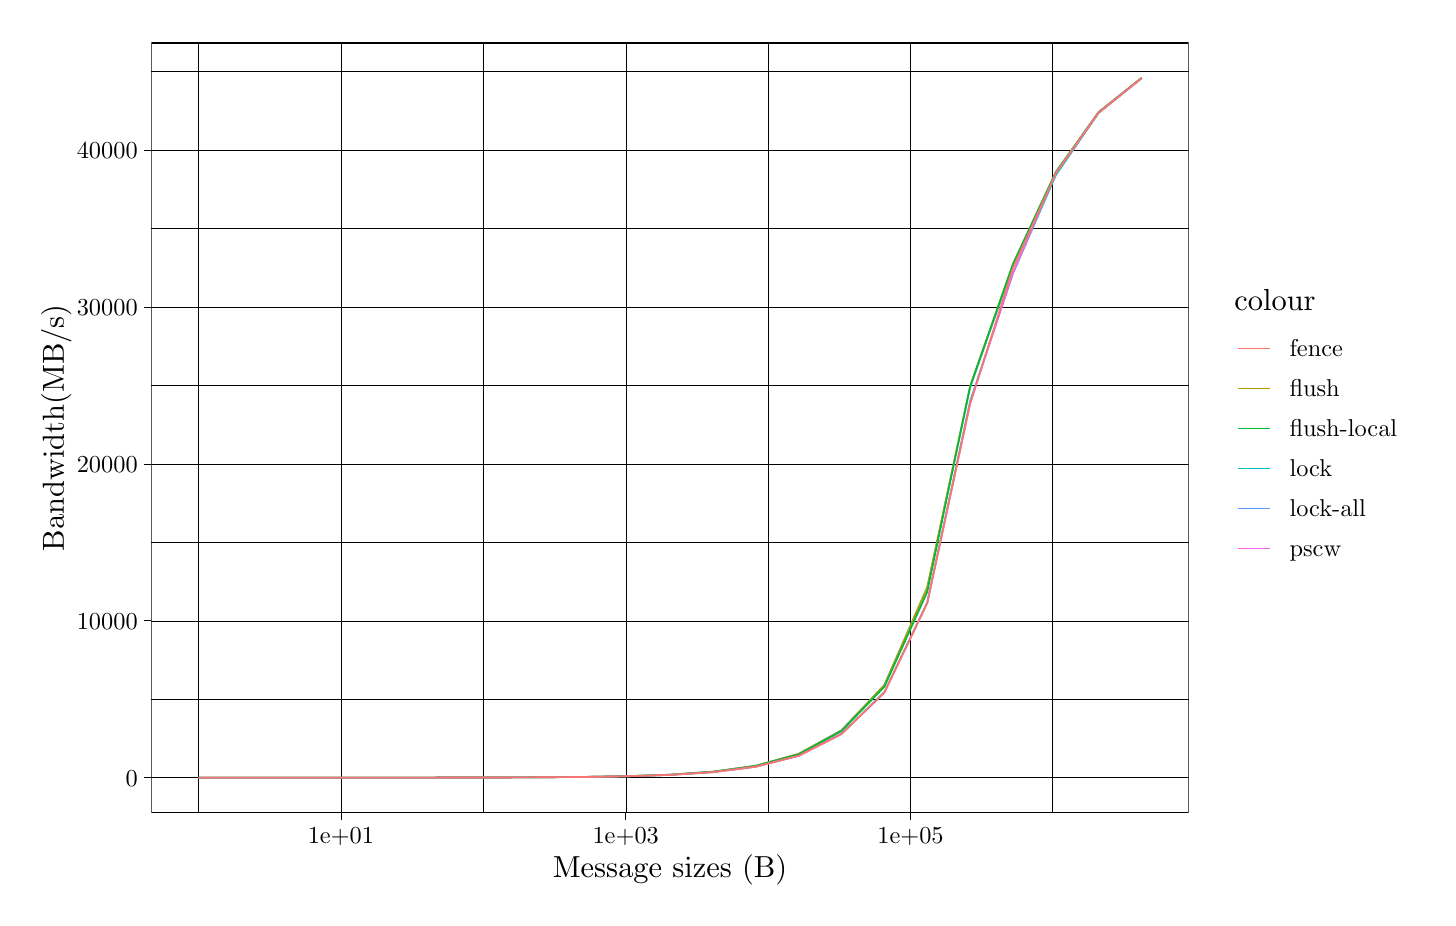
\begin{tikzpicture}[x=1pt,y=1pt]
\definecolor{fillColor}{RGB}{255,255,255}
\path[use as bounding box,fill=fillColor,fill opacity=0.00] (0,0) rectangle (505.89,314.37);
\begin{scope}
\path[clip] (  0.00,  0.00) rectangle (505.89,314.37);
\definecolor{drawColor}{RGB}{255,255,255}
\definecolor{fillColor}{RGB}{255,255,255}

\path[draw=drawColor,line width= 0.6pt,line join=round,line cap=round,fill=fillColor] (  0.00,  0.00) rectangle (505.89,314.37);
\end{scope}
\begin{scope}
\path[clip] ( 44.71, 30.72) rectangle (419.53,308.87);
\definecolor{fillColor}{RGB}{255,255,255}

\path[fill=fillColor] ( 44.71, 30.72) rectangle (419.53,308.87);
\definecolor{drawColor}{RGB}{0,0,0}

\path[draw=drawColor,line width= 0.0pt,line join=round] ( 44.71, 71.70) --
	(419.53, 71.70);

\path[draw=drawColor,line width= 0.0pt,line join=round] ( 44.71,128.36) --
	(419.53,128.36);

\path[draw=drawColor,line width= 0.0pt,line join=round] ( 44.71,185.02) --
	(419.53,185.02);

\path[draw=drawColor,line width= 0.0pt,line join=round] ( 44.71,241.68) --
	(419.53,241.68);

\path[draw=drawColor,line width= 0.0pt,line join=round] ( 44.71,298.35) --
	(419.53,298.35);

\path[draw=drawColor,line width= 0.0pt,line join=round] ( 61.75, 30.72) --
	( 61.75,308.87);

\path[draw=drawColor,line width= 0.0pt,line join=round] (164.65, 30.72) --
	(164.65,308.87);

\path[draw=drawColor,line width= 0.0pt,line join=round] (267.55, 30.72) --
	(267.55,308.87);

\path[draw=drawColor,line width= 0.0pt,line join=round] (370.46, 30.72) --
	(370.46,308.87);

\path[draw=drawColor,line width= 0.1pt,line join=round] ( 44.71, 43.37) --
	(419.53, 43.37);

\path[draw=drawColor,line width= 0.1pt,line join=round] ( 44.71,100.03) --
	(419.53,100.03);

\path[draw=drawColor,line width= 0.1pt,line join=round] ( 44.71,156.69) --
	(419.53,156.69);

\path[draw=drawColor,line width= 0.1pt,line join=round] ( 44.71,213.35) --
	(419.53,213.35);

\path[draw=drawColor,line width= 0.1pt,line join=round] ( 44.71,270.02) --
	(419.53,270.02);

\path[draw=drawColor,line width= 0.1pt,line join=round] (113.20, 30.72) --
	(113.20,308.87);

\path[draw=drawColor,line width= 0.1pt,line join=round] (216.10, 30.72) --
	(216.10,308.87);

\path[draw=drawColor,line width= 0.1pt,line join=round] (319.01, 30.72) --
	(319.01,308.87);
\definecolor{drawColor}{RGB}{97,156,255}

\path[draw=drawColor,line width= 0.6pt,line join=round] ( 61.75, 43.37) --
	( 77.24, 43.37) --
	( 92.73, 43.37) --
	(108.22, 43.37) --
	(123.70, 43.38) --
	(139.19, 43.38) --
	(154.68, 43.40) --
	(170.17, 43.43) --
	(185.66, 43.50) --
	(201.15, 43.64) --
	(216.63, 43.90) --
	(232.12, 44.44) --
	(247.61, 45.52) --
	(263.10, 47.66) --
	(278.59, 51.96) --
	(294.08, 60.52) --
	(309.56, 76.84) --
	(325.05,112.12) --
	(340.54,184.33) --
	(356.03,228.24) --
	(371.52,261.69) --
	(387.00,283.58) --
	(402.49,296.05);
\definecolor{drawColor}{RGB}{0,191,196}

\path[draw=drawColor,line width= 0.6pt,line join=round] ( 61.75, 43.37) --
	( 77.24, 43.37) --
	( 92.73, 43.37) --
	(108.22, 43.37) --
	(123.70, 43.38) --
	(139.19, 43.38) --
	(154.68, 43.40) --
	(170.17, 43.43) --
	(185.66, 43.49) --
	(201.15, 43.62) --
	(216.63, 43.86) --
	(232.12, 44.36) --
	(247.61, 45.36) --
	(263.10, 47.33) --
	(278.59, 51.31) --
	(294.08, 59.27) --
	(309.56, 74.29) --
	(325.05,106.62) --
	(340.54,179.36) --
	(356.03,225.59) --
	(371.52,261.07) --
	(387.00,283.63) --
	(402.49,296.09);
\definecolor{drawColor}{RGB}{183,159,0}

\path[draw=drawColor,line width= 0.6pt,line join=round] ( 61.75, 43.37) --
	( 77.24, 43.37) --
	( 92.73, 43.37) --
	(108.22, 43.37) --
	(123.70, 43.38) --
	(139.19, 43.38) --
	(154.68, 43.40) --
	(170.17, 43.43) --
	(185.66, 43.50) --
	(201.15, 43.64) --
	(216.63, 43.91) --
	(232.12, 44.44) --
	(247.61, 45.52) --
	(263.10, 47.67) --
	(278.59, 51.95) --
	(294.08, 60.43) --
	(309.56, 76.82) --
	(325.05,112.08) --
	(340.54,184.87) --
	(356.03,228.92) --
	(371.52,262.20) --
	(387.00,283.89) --
	(402.49,296.23);
\definecolor{drawColor}{RGB}{0,186,56}

\path[draw=drawColor,line width= 0.6pt,line join=round] ( 61.75, 43.37) --
	( 77.24, 43.37) --
	( 92.73, 43.37) --
	(108.22, 43.37) --
	(123.70, 43.38) --
	(139.19, 43.38) --
	(154.68, 43.40) --
	(170.17, 43.43) --
	(185.66, 43.50) --
	(201.15, 43.63) --
	(216.63, 43.89) --
	(232.12, 44.42) --
	(247.61, 45.49) --
	(263.10, 47.59) --
	(278.59, 51.77) --
	(294.08, 60.20) --
	(309.56, 76.19) --
	(325.05,110.43) --
	(340.54,184.61) --
	(356.03,228.96) --
	(371.52,262.18) --
	(387.00,283.87) --
	(402.49,296.22);
\definecolor{drawColor}{RGB}{245,100,227}

\path[draw=drawColor,line width= 0.6pt,line join=round] ( 61.75, 43.37) --
	( 77.24, 43.37) --
	( 92.73, 43.37) --
	(108.22, 43.37) --
	(123.70, 43.38) --
	(139.19, 43.38) --
	(154.68, 43.40) --
	(170.17, 43.43) --
	(185.66, 43.49) --
	(201.15, 43.62) --
	(216.63, 43.86) --
	(232.12, 44.36) --
	(247.61, 45.35) --
	(263.10, 47.32) --
	(278.59, 51.27) --
	(294.08, 59.23) --
	(309.56, 74.08) --
	(325.05,106.51) --
	(340.54,178.77) --
	(356.03,225.70) --
	(371.52,261.82) --
	(387.00,283.74) --
	(402.49,296.13);
\definecolor{drawColor}{RGB}{248,118,109}

\path[draw=drawColor,line width= 0.6pt,line join=round] ( 61.75, 43.37) --
	( 77.24, 43.37) --
	( 92.73, 43.37) --
	(108.22, 43.37) --
	(123.70, 43.38) --
	(139.19, 43.38) --
	(154.68, 43.40) --
	(170.17, 43.43) --
	(185.66, 43.49) --
	(201.15, 43.61) --
	(216.63, 43.86) --
	(232.12, 44.35) --
	(247.61, 45.34) --
	(263.10, 47.31) --
	(278.59, 51.25) --
	(294.08, 59.08) --
	(309.56, 74.12) --
	(325.05,106.39) --
	(340.54,178.29) --
	(356.03,227.55) --
	(371.52,261.74) --
	(387.00,283.62) --
	(402.49,296.08);
\definecolor{drawColor}{RGB}{0,0,0}

\path[draw=drawColor,line width= 0.6pt,line join=round,line cap=round] ( 44.71, 30.72) rectangle (419.53,308.87);
\end{scope}
\begin{scope}
\path[clip] (  0.00,  0.00) rectangle (505.89,314.37);
\definecolor{drawColor}{RGB}{0,0,0}

\node[text=drawColor,anchor=base east,inner sep=0pt, outer sep=0pt, scale=  0.88] at ( 39.76, 40.34) {0};

\node[text=drawColor,anchor=base east,inner sep=0pt, outer sep=0pt, scale=  0.88] at ( 39.76, 97.00) {10000};

\node[text=drawColor,anchor=base east,inner sep=0pt, outer sep=0pt, scale=  0.88] at ( 39.76,153.66) {20000};

\node[text=drawColor,anchor=base east,inner sep=0pt, outer sep=0pt, scale=  0.88] at ( 39.76,210.32) {30000};

\node[text=drawColor,anchor=base east,inner sep=0pt, outer sep=0pt, scale=  0.88] at ( 39.76,266.99) {40000};
\end{scope}
\begin{scope}
\path[clip] (  0.00,  0.00) rectangle (505.89,314.37);
\definecolor{drawColor}{RGB}{0,0,0}

\path[draw=drawColor,line width= 0.3pt,line join=round] ( 41.96, 43.37) --
	( 44.71, 43.37);

\path[draw=drawColor,line width= 0.3pt,line join=round] ( 41.96,100.03) --
	( 44.71,100.03);

\path[draw=drawColor,line width= 0.3pt,line join=round] ( 41.96,156.69) --
	( 44.71,156.69);

\path[draw=drawColor,line width= 0.3pt,line join=round] ( 41.96,213.35) --
	( 44.71,213.35);

\path[draw=drawColor,line width= 0.3pt,line join=round] ( 41.96,270.02) --
	( 44.71,270.02);
\end{scope}
\begin{scope}
\path[clip] (  0.00,  0.00) rectangle (505.89,314.37);
\definecolor{drawColor}{RGB}{0,0,0}

\path[draw=drawColor,line width= 0.3pt,line join=round] (113.20, 27.97) --
	(113.20, 30.72);

\path[draw=drawColor,line width= 0.3pt,line join=round] (216.10, 27.97) --
	(216.10, 30.72);

\path[draw=drawColor,line width= 0.3pt,line join=round] (319.01, 27.97) --
	(319.01, 30.72);
\end{scope}
\begin{scope}
\path[clip] (  0.00,  0.00) rectangle (505.89,314.37);
\definecolor{drawColor}{RGB}{0,0,0}

\node[text=drawColor,anchor=base,inner sep=0pt, outer sep=0pt, scale=  0.88] at (113.20, 19.71) {1e+01};

\node[text=drawColor,anchor=base,inner sep=0pt, outer sep=0pt, scale=  0.88] at (216.10, 19.71) {1e+03};

\node[text=drawColor,anchor=base,inner sep=0pt, outer sep=0pt, scale=  0.88] at (319.01, 19.71) {1e+05};
\end{scope}
\begin{scope}
\path[clip] (  0.00,  0.00) rectangle (505.89,314.37);
\definecolor{drawColor}{RGB}{0,0,0}

\node[text=drawColor,anchor=base,inner sep=0pt, outer sep=0pt, scale=  1.10] at (232.12,  7.44) {Message sizes (B)};
\end{scope}
\begin{scope}
\path[clip] (  0.00,  0.00) rectangle (505.89,314.37);
\definecolor{drawColor}{RGB}{0,0,0}

\node[text=drawColor,rotate= 90.00,anchor=base,inner sep=0pt, outer sep=0pt, scale=  1.10] at ( 13.08,169.80) {Bandwidth(MB/s)};
\end{scope}
\begin{scope}
\path[clip] (  0.00,  0.00) rectangle (505.89,314.37);
\definecolor{fillColor}{RGB}{255,255,255}

\path[fill=fillColor] (430.53,113.43) rectangle (500.39,226.17);
\end{scope}
\begin{scope}
\path[clip] (  0.00,  0.00) rectangle (505.89,314.37);
\definecolor{drawColor}{RGB}{0,0,0}

\node[text=drawColor,anchor=base west,inner sep=0pt, outer sep=0pt, scale=  1.10] at (436.03,212.12) {colour};
\end{scope}
\begin{scope}
\path[clip] (  0.00,  0.00) rectangle (505.89,314.37);
\definecolor{fillColor}{RGB}{255,255,255}

\path[fill=fillColor] (436.03,191.20) rectangle (450.48,205.65);
\end{scope}
\begin{scope}
\path[clip] (  0.00,  0.00) rectangle (505.89,314.37);
\definecolor{drawColor}{RGB}{248,118,109}

\path[draw=drawColor,line width= 0.6pt,line join=round] (437.48,198.42) -- (449.04,198.42);
\end{scope}
\begin{scope}
\path[clip] (  0.00,  0.00) rectangle (505.89,314.37);
\definecolor{drawColor}{RGB}{248,118,109}

\path[draw=drawColor,line width= 0.6pt,line join=round] (437.48,198.42) -- (449.04,198.42);
\end{scope}
\begin{scope}
\path[clip] (  0.00,  0.00) rectangle (505.89,314.37);
\definecolor{drawColor}{RGB}{248,118,109}

\path[draw=drawColor,line width= 0.6pt,line join=round] (437.48,198.42) -- (449.04,198.42);
\end{scope}
\begin{scope}
\path[clip] (  0.00,  0.00) rectangle (505.89,314.37);
\definecolor{drawColor}{RGB}{248,118,109}

\path[draw=drawColor,line width= 0.6pt,line join=round] (437.48,198.42) -- (449.04,198.42);
\end{scope}
\begin{scope}
\path[clip] (  0.00,  0.00) rectangle (505.89,314.37);
\definecolor{drawColor}{RGB}{248,118,109}

\path[draw=drawColor,line width= 0.6pt,line join=round] (437.48,198.42) -- (449.04,198.42);
\end{scope}
\begin{scope}
\path[clip] (  0.00,  0.00) rectangle (505.89,314.37);
\definecolor{drawColor}{RGB}{248,118,109}

\path[draw=drawColor,line width= 0.6pt,line join=round] (437.48,198.42) -- (449.04,198.42);
\end{scope}
\begin{scope}
\path[clip] (  0.00,  0.00) rectangle (505.89,314.37);
\definecolor{fillColor}{RGB}{255,255,255}

\path[fill=fillColor] (436.03,176.74) rectangle (450.48,191.20);
\end{scope}
\begin{scope}
\path[clip] (  0.00,  0.00) rectangle (505.89,314.37);
\definecolor{drawColor}{RGB}{183,159,0}

\path[draw=drawColor,line width= 0.6pt,line join=round] (437.48,183.97) -- (449.04,183.97);
\end{scope}
\begin{scope}
\path[clip] (  0.00,  0.00) rectangle (505.89,314.37);
\definecolor{drawColor}{RGB}{183,159,0}

\path[draw=drawColor,line width= 0.6pt,line join=round] (437.48,183.97) -- (449.04,183.97);
\end{scope}
\begin{scope}
\path[clip] (  0.00,  0.00) rectangle (505.89,314.37);
\definecolor{drawColor}{RGB}{183,159,0}

\path[draw=drawColor,line width= 0.6pt,line join=round] (437.48,183.97) -- (449.04,183.97);
\end{scope}
\begin{scope}
\path[clip] (  0.00,  0.00) rectangle (505.89,314.37);
\definecolor{drawColor}{RGB}{183,159,0}

\path[draw=drawColor,line width= 0.6pt,line join=round] (437.48,183.97) -- (449.04,183.97);
\end{scope}
\begin{scope}
\path[clip] (  0.00,  0.00) rectangle (505.89,314.37);
\definecolor{drawColor}{RGB}{183,159,0}

\path[draw=drawColor,line width= 0.6pt,line join=round] (437.48,183.97) -- (449.04,183.97);
\end{scope}
\begin{scope}
\path[clip] (  0.00,  0.00) rectangle (505.89,314.37);
\definecolor{drawColor}{RGB}{183,159,0}

\path[draw=drawColor,line width= 0.6pt,line join=round] (437.48,183.97) -- (449.04,183.97);
\end{scope}
\begin{scope}
\path[clip] (  0.00,  0.00) rectangle (505.89,314.37);
\definecolor{fillColor}{RGB}{255,255,255}

\path[fill=fillColor] (436.03,162.29) rectangle (450.48,176.74);
\end{scope}
\begin{scope}
\path[clip] (  0.00,  0.00) rectangle (505.89,314.37);
\definecolor{drawColor}{RGB}{0,186,56}

\path[draw=drawColor,line width= 0.6pt,line join=round] (437.48,169.52) -- (449.04,169.52);
\end{scope}
\begin{scope}
\path[clip] (  0.00,  0.00) rectangle (505.89,314.37);
\definecolor{drawColor}{RGB}{0,186,56}

\path[draw=drawColor,line width= 0.6pt,line join=round] (437.48,169.52) -- (449.04,169.52);
\end{scope}
\begin{scope}
\path[clip] (  0.00,  0.00) rectangle (505.89,314.37);
\definecolor{drawColor}{RGB}{0,186,56}

\path[draw=drawColor,line width= 0.6pt,line join=round] (437.48,169.52) -- (449.04,169.52);
\end{scope}
\begin{scope}
\path[clip] (  0.00,  0.00) rectangle (505.89,314.37);
\definecolor{drawColor}{RGB}{0,186,56}

\path[draw=drawColor,line width= 0.6pt,line join=round] (437.48,169.52) -- (449.04,169.52);
\end{scope}
\begin{scope}
\path[clip] (  0.00,  0.00) rectangle (505.89,314.37);
\definecolor{drawColor}{RGB}{0,186,56}

\path[draw=drawColor,line width= 0.6pt,line join=round] (437.48,169.52) -- (449.04,169.52);
\end{scope}
\begin{scope}
\path[clip] (  0.00,  0.00) rectangle (505.89,314.37);
\definecolor{drawColor}{RGB}{0,186,56}

\path[draw=drawColor,line width= 0.6pt,line join=round] (437.48,169.52) -- (449.04,169.52);
\end{scope}
\begin{scope}
\path[clip] (  0.00,  0.00) rectangle (505.89,314.37);
\definecolor{fillColor}{RGB}{255,255,255}

\path[fill=fillColor] (436.03,147.84) rectangle (450.48,162.29);
\end{scope}
\begin{scope}
\path[clip] (  0.00,  0.00) rectangle (505.89,314.37);
\definecolor{drawColor}{RGB}{0,191,196}

\path[draw=drawColor,line width= 0.6pt,line join=round] (437.48,155.06) -- (449.04,155.06);
\end{scope}
\begin{scope}
\path[clip] (  0.00,  0.00) rectangle (505.89,314.37);
\definecolor{drawColor}{RGB}{0,191,196}

\path[draw=drawColor,line width= 0.6pt,line join=round] (437.48,155.06) -- (449.04,155.06);
\end{scope}
\begin{scope}
\path[clip] (  0.00,  0.00) rectangle (505.89,314.37);
\definecolor{drawColor}{RGB}{0,191,196}

\path[draw=drawColor,line width= 0.6pt,line join=round] (437.48,155.06) -- (449.04,155.06);
\end{scope}
\begin{scope}
\path[clip] (  0.00,  0.00) rectangle (505.89,314.37);
\definecolor{drawColor}{RGB}{0,191,196}

\path[draw=drawColor,line width= 0.6pt,line join=round] (437.48,155.06) -- (449.04,155.06);
\end{scope}
\begin{scope}
\path[clip] (  0.00,  0.00) rectangle (505.89,314.37);
\definecolor{drawColor}{RGB}{0,191,196}

\path[draw=drawColor,line width= 0.6pt,line join=round] (437.48,155.06) -- (449.04,155.06);
\end{scope}
\begin{scope}
\path[clip] (  0.00,  0.00) rectangle (505.89,314.37);
\definecolor{drawColor}{RGB}{0,191,196}

\path[draw=drawColor,line width= 0.6pt,line join=round] (437.48,155.06) -- (449.04,155.06);
\end{scope}
\begin{scope}
\path[clip] (  0.00,  0.00) rectangle (505.89,314.37);
\definecolor{fillColor}{RGB}{255,255,255}

\path[fill=fillColor] (436.03,133.38) rectangle (450.48,147.84);
\end{scope}
\begin{scope}
\path[clip] (  0.00,  0.00) rectangle (505.89,314.37);
\definecolor{drawColor}{RGB}{97,156,255}

\path[draw=drawColor,line width= 0.6pt,line join=round] (437.48,140.61) -- (449.04,140.61);
\end{scope}
\begin{scope}
\path[clip] (  0.00,  0.00) rectangle (505.89,314.37);
\definecolor{drawColor}{RGB}{97,156,255}

\path[draw=drawColor,line width= 0.6pt,line join=round] (437.48,140.61) -- (449.04,140.61);
\end{scope}
\begin{scope}
\path[clip] (  0.00,  0.00) rectangle (505.89,314.37);
\definecolor{drawColor}{RGB}{97,156,255}

\path[draw=drawColor,line width= 0.6pt,line join=round] (437.48,140.61) -- (449.04,140.61);
\end{scope}
\begin{scope}
\path[clip] (  0.00,  0.00) rectangle (505.89,314.37);
\definecolor{drawColor}{RGB}{97,156,255}

\path[draw=drawColor,line width= 0.6pt,line join=round] (437.48,140.61) -- (449.04,140.61);
\end{scope}
\begin{scope}
\path[clip] (  0.00,  0.00) rectangle (505.89,314.37);
\definecolor{drawColor}{RGB}{97,156,255}

\path[draw=drawColor,line width= 0.6pt,line join=round] (437.48,140.61) -- (449.04,140.61);
\end{scope}
\begin{scope}
\path[clip] (  0.00,  0.00) rectangle (505.89,314.37);
\definecolor{drawColor}{RGB}{97,156,255}

\path[draw=drawColor,line width= 0.6pt,line join=round] (437.48,140.61) -- (449.04,140.61);
\end{scope}
\begin{scope}
\path[clip] (  0.00,  0.00) rectangle (505.89,314.37);
\definecolor{fillColor}{RGB}{255,255,255}

\path[fill=fillColor] (436.03,118.93) rectangle (450.48,133.38);
\end{scope}
\begin{scope}
\path[clip] (  0.00,  0.00) rectangle (505.89,314.37);
\definecolor{drawColor}{RGB}{245,100,227}

\path[draw=drawColor,line width= 0.6pt,line join=round] (437.48,126.15) -- (449.04,126.15);
\end{scope}
\begin{scope}
\path[clip] (  0.00,  0.00) rectangle (505.89,314.37);
\definecolor{drawColor}{RGB}{245,100,227}

\path[draw=drawColor,line width= 0.6pt,line join=round] (437.48,126.15) -- (449.04,126.15);
\end{scope}
\begin{scope}
\path[clip] (  0.00,  0.00) rectangle (505.89,314.37);
\definecolor{drawColor}{RGB}{245,100,227}

\path[draw=drawColor,line width= 0.6pt,line join=round] (437.48,126.15) -- (449.04,126.15);
\end{scope}
\begin{scope}
\path[clip] (  0.00,  0.00) rectangle (505.89,314.37);
\definecolor{drawColor}{RGB}{245,100,227}

\path[draw=drawColor,line width= 0.6pt,line join=round] (437.48,126.15) -- (449.04,126.15);
\end{scope}
\begin{scope}
\path[clip] (  0.00,  0.00) rectangle (505.89,314.37);
\definecolor{drawColor}{RGB}{245,100,227}

\path[draw=drawColor,line width= 0.6pt,line join=round] (437.48,126.15) -- (449.04,126.15);
\end{scope}
\begin{scope}
\path[clip] (  0.00,  0.00) rectangle (505.89,314.37);
\definecolor{drawColor}{RGB}{245,100,227}

\path[draw=drawColor,line width= 0.6pt,line join=round] (437.48,126.15) -- (449.04,126.15);
\end{scope}
\begin{scope}
\path[clip] (  0.00,  0.00) rectangle (505.89,314.37);
\definecolor{drawColor}{RGB}{0,0,0}

\node[text=drawColor,anchor=base west,inner sep=0pt, outer sep=0pt, scale=  0.88] at (455.98,195.39) {fence};
\end{scope}
\begin{scope}
\path[clip] (  0.00,  0.00) rectangle (505.89,314.37);
\definecolor{drawColor}{RGB}{0,0,0}

\node[text=drawColor,anchor=base west,inner sep=0pt, outer sep=0pt, scale=  0.88] at (455.98,180.94) {flush};
\end{scope}
\begin{scope}
\path[clip] (  0.00,  0.00) rectangle (505.89,314.37);
\definecolor{drawColor}{RGB}{0,0,0}

\node[text=drawColor,anchor=base west,inner sep=0pt, outer sep=0pt, scale=  0.88] at (455.98,166.49) {flush-local};
\end{scope}
\begin{scope}
\path[clip] (  0.00,  0.00) rectangle (505.89,314.37);
\definecolor{drawColor}{RGB}{0,0,0}

\node[text=drawColor,anchor=base west,inner sep=0pt, outer sep=0pt, scale=  0.88] at (455.98,152.03) {lock};
\end{scope}
\begin{scope}
\path[clip] (  0.00,  0.00) rectangle (505.89,314.37);
\definecolor{drawColor}{RGB}{0,0,0}

\node[text=drawColor,anchor=base west,inner sep=0pt, outer sep=0pt, scale=  0.88] at (455.98,137.58) {lock-all};
\end{scope}
\begin{scope}
\path[clip] (  0.00,  0.00) rectangle (505.89,314.37);
\definecolor{drawColor}{RGB}{0,0,0}

\node[text=drawColor,anchor=base west,inner sep=0pt, outer sep=0pt, scale=  0.88] at (455.98,123.12) {pscw};
\end{scope}
\end{tikzpicture}

	\caption{1 node, get bw, gpu-gpu, window create, sync algorithm comparisons}
\end{figure}

\begin{figure}
	% Created by tikzDevice version 0.10.1 on 2020-02-15 16:01:12
% !TEX encoding = UTF-8 Unicode
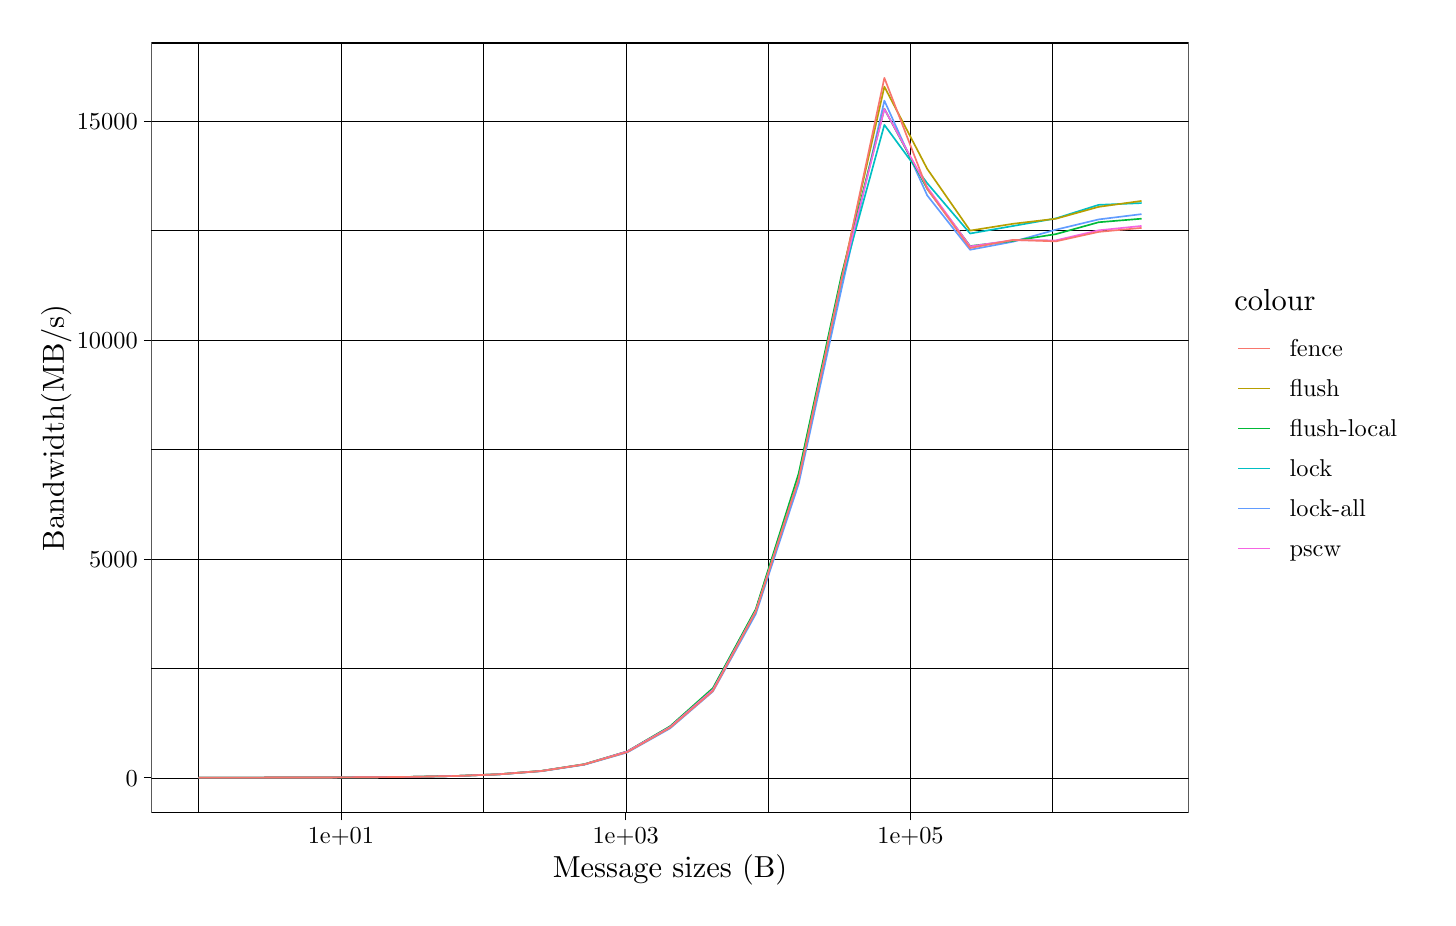
\begin{tikzpicture}[x=1pt,y=1pt]
\definecolor{fillColor}{RGB}{255,255,255}
\path[use as bounding box,fill=fillColor,fill opacity=0.00] (0,0) rectangle (505.89,314.37);
\begin{scope}
\path[clip] (  0.00,  0.00) rectangle (505.89,314.37);
\definecolor{drawColor}{RGB}{255,255,255}
\definecolor{fillColor}{RGB}{255,255,255}

\path[draw=drawColor,line width= 0.6pt,line join=round,line cap=round,fill=fillColor] (  0.00,  0.00) rectangle (505.89,314.37);
\end{scope}
\begin{scope}
\path[clip] ( 44.71, 30.72) rectangle (419.53,308.87);
\definecolor{fillColor}{RGB}{255,255,255}

\path[fill=fillColor] ( 44.71, 30.72) rectangle (419.53,308.87);
\definecolor{drawColor}{RGB}{0,0,0}

\path[draw=drawColor,line width= 0.0pt,line join=round] ( 44.71, 82.88) --
	(419.53, 82.88);

\path[draw=drawColor,line width= 0.0pt,line join=round] ( 44.71,161.91) --
	(419.53,161.91);

\path[draw=drawColor,line width= 0.0pt,line join=round] ( 44.71,240.94) --
	(419.53,240.94);

\path[draw=drawColor,line width= 0.0pt,line join=round] ( 61.75, 30.72) --
	( 61.75,308.87);

\path[draw=drawColor,line width= 0.0pt,line join=round] (164.65, 30.72) --
	(164.65,308.87);

\path[draw=drawColor,line width= 0.0pt,line join=round] (267.55, 30.72) --
	(267.55,308.87);

\path[draw=drawColor,line width= 0.0pt,line join=round] (370.46, 30.72) --
	(370.46,308.87);

\path[draw=drawColor,line width= 0.1pt,line join=round] ( 44.71, 43.36) --
	(419.53, 43.36);

\path[draw=drawColor,line width= 0.1pt,line join=round] ( 44.71,122.39) --
	(419.53,122.39);

\path[draw=drawColor,line width= 0.1pt,line join=round] ( 44.71,201.42) --
	(419.53,201.42);

\path[draw=drawColor,line width= 0.1pt,line join=round] ( 44.71,280.46) --
	(419.53,280.46);

\path[draw=drawColor,line width= 0.1pt,line join=round] (113.20, 30.72) --
	(113.20,308.87);

\path[draw=drawColor,line width= 0.1pt,line join=round] (216.10, 30.72) --
	(216.10,308.87);

\path[draw=drawColor,line width= 0.1pt,line join=round] (319.01, 30.72) --
	(319.01,308.87);
\definecolor{drawColor}{RGB}{97,156,255}

\path[draw=drawColor,line width= 0.6pt,line join=round] ( 61.75, 43.37) --
	( 77.24, 43.38) --
	( 92.73, 43.40) --
	(108.22, 43.43) --
	(123.70, 43.51) --
	(139.19, 43.66) --
	(154.68, 43.95) --
	(170.17, 44.54) --
	(185.66, 45.71) --
	(201.15, 48.04) --
	(216.63, 52.47) --
	(232.12, 61.17) --
	(247.61, 74.52) --
	(263.10,102.50) --
	(278.59,149.54) --
	(294.08,219.96) --
	(309.56,287.99) --
	(325.05,253.75) --
	(340.54,234.12) --
	(356.03,237.02) --
	(371.52,241.36) --
	(387.00,245.08) --
	(402.49,246.99);
\definecolor{drawColor}{RGB}{0,191,196}

\path[draw=drawColor,line width= 0.6pt,line join=round] ( 61.75, 43.37) --
	( 77.24, 43.38) --
	( 92.73, 43.40) --
	(108.22, 43.44) --
	(123.70, 43.51) --
	(139.19, 43.66) --
	(154.68, 43.96) --
	(170.17, 44.56) --
	(185.66, 45.76) --
	(201.15, 48.13) --
	(216.63, 52.67) --
	(232.12, 61.49) --
	(247.61, 75.02) --
	(263.10,103.29) --
	(278.59,151.19) --
	(294.08,222.60) --
	(309.56,279.24) --
	(325.05,258.16) --
	(340.54,239.99) --
	(356.03,242.70) --
	(371.52,245.44) --
	(387.00,250.34) --
	(402.49,250.99);
\definecolor{drawColor}{RGB}{183,159,0}

\path[draw=drawColor,line width= 0.6pt,line join=round] ( 61.75, 43.37) --
	( 77.24, 43.38) --
	( 92.73, 43.40) --
	(108.22, 43.44) --
	(123.70, 43.51) --
	(139.19, 43.66) --
	(154.68, 43.97) --
	(170.17, 44.58) --
	(185.66, 45.79) --
	(201.15, 48.19) --
	(216.63, 52.82) --
	(232.12, 61.73) --
	(247.61, 75.37) --
	(263.10,103.93) --
	(278.59,152.37) --
	(294.08,224.02) --
	(309.56,293.05) --
	(325.05,263.34) --
	(340.54,241.04) --
	(356.03,243.50) --
	(371.52,245.32) --
	(387.00,249.62) --
	(402.49,251.76);
\definecolor{drawColor}{RGB}{0,186,56}

\path[draw=drawColor,line width= 0.6pt,line join=round] ( 61.75, 43.37) --
	( 77.24, 43.38) --
	( 92.73, 43.40) --
	(108.22, 43.44) --
	(123.70, 43.51) --
	(139.19, 43.67) --
	(154.68, 43.98) --
	(170.17, 44.59) --
	(185.66, 45.82) --
	(201.15, 48.23) --
	(216.63, 52.84) --
	(232.12, 61.92) --
	(247.61, 75.72) --
	(263.10,104.26) --
	(278.59,153.25) --
	(294.08,224.93) --
	(309.56,285.05) --
	(325.05,256.13) --
	(340.54,235.46) --
	(356.03,237.31) --
	(371.52,239.76) --
	(387.00,244.06) --
	(402.49,245.34);
\definecolor{drawColor}{RGB}{245,100,227}

\path[draw=drawColor,line width= 0.6pt,line join=round] ( 61.75, 43.37) --
	( 77.24, 43.38) --
	( 92.73, 43.40) --
	(108.22, 43.44) --
	(123.70, 43.51) --
	(139.19, 43.66) --
	(154.68, 43.97) --
	(170.17, 44.58) --
	(185.66, 45.79) --
	(201.15, 48.18) --
	(216.63, 52.81) --
	(232.12, 61.65) --
	(247.61, 75.11) --
	(263.10,103.58) --
	(278.59,151.21) --
	(294.08,223.32) --
	(309.56,284.99) --
	(325.05,256.71) --
	(340.54,235.32) --
	(356.03,237.58) --
	(371.52,237.51) --
	(387.00,241.14) --
	(402.49,242.72);
\definecolor{drawColor}{RGB}{248,118,109}

\path[draw=drawColor,line width= 0.6pt,line join=round] ( 61.75, 43.37) --
	( 77.24, 43.38) --
	( 92.73, 43.40) --
	(108.22, 43.43) --
	(123.70, 43.51) --
	(139.19, 43.66) --
	(154.68, 43.96) --
	(170.17, 44.56) --
	(185.66, 45.76) --
	(201.15, 48.14) --
	(216.63, 52.58) --
	(232.12, 61.40) --
	(247.61, 74.68) --
	(263.10,103.33) --
	(278.59,151.27) --
	(294.08,223.22) --
	(309.56,296.23) --
	(325.05,256.10) --
	(340.54,234.73) --
	(356.03,237.68) --
	(371.52,237.15) --
	(387.00,240.58) --
	(402.49,242.01);
\definecolor{drawColor}{RGB}{0,0,0}

\path[draw=drawColor,line width= 0.6pt,line join=round,line cap=round] ( 44.71, 30.72) rectangle (419.53,308.87);
\end{scope}
\begin{scope}
\path[clip] (  0.00,  0.00) rectangle (505.89,314.37);
\definecolor{drawColor}{RGB}{0,0,0}

\node[text=drawColor,anchor=base east,inner sep=0pt, outer sep=0pt, scale=  0.88] at ( 39.76, 40.33) {0};

\node[text=drawColor,anchor=base east,inner sep=0pt, outer sep=0pt, scale=  0.88] at ( 39.76,119.36) {5000};

\node[text=drawColor,anchor=base east,inner sep=0pt, outer sep=0pt, scale=  0.88] at ( 39.76,198.39) {10000};

\node[text=drawColor,anchor=base east,inner sep=0pt, outer sep=0pt, scale=  0.88] at ( 39.76,277.43) {15000};
\end{scope}
\begin{scope}
\path[clip] (  0.00,  0.00) rectangle (505.89,314.37);
\definecolor{drawColor}{RGB}{0,0,0}

\path[draw=drawColor,line width= 0.3pt,line join=round] ( 41.96, 43.36) --
	( 44.71, 43.36);

\path[draw=drawColor,line width= 0.3pt,line join=round] ( 41.96,122.39) --
	( 44.71,122.39);

\path[draw=drawColor,line width= 0.3pt,line join=round] ( 41.96,201.42) --
	( 44.71,201.42);

\path[draw=drawColor,line width= 0.3pt,line join=round] ( 41.96,280.46) --
	( 44.71,280.46);
\end{scope}
\begin{scope}
\path[clip] (  0.00,  0.00) rectangle (505.89,314.37);
\definecolor{drawColor}{RGB}{0,0,0}

\path[draw=drawColor,line width= 0.3pt,line join=round] (113.20, 27.97) --
	(113.20, 30.72);

\path[draw=drawColor,line width= 0.3pt,line join=round] (216.10, 27.97) --
	(216.10, 30.72);

\path[draw=drawColor,line width= 0.3pt,line join=round] (319.01, 27.97) --
	(319.01, 30.72);
\end{scope}
\begin{scope}
\path[clip] (  0.00,  0.00) rectangle (505.89,314.37);
\definecolor{drawColor}{RGB}{0,0,0}

\node[text=drawColor,anchor=base,inner sep=0pt, outer sep=0pt, scale=  0.88] at (113.20, 19.71) {1e+01};

\node[text=drawColor,anchor=base,inner sep=0pt, outer sep=0pt, scale=  0.88] at (216.10, 19.71) {1e+03};

\node[text=drawColor,anchor=base,inner sep=0pt, outer sep=0pt, scale=  0.88] at (319.01, 19.71) {1e+05};
\end{scope}
\begin{scope}
\path[clip] (  0.00,  0.00) rectangle (505.89,314.37);
\definecolor{drawColor}{RGB}{0,0,0}

\node[text=drawColor,anchor=base,inner sep=0pt, outer sep=0pt, scale=  1.10] at (232.12,  7.44) {Message sizes (B)};
\end{scope}
\begin{scope}
\path[clip] (  0.00,  0.00) rectangle (505.89,314.37);
\definecolor{drawColor}{RGB}{0,0,0}

\node[text=drawColor,rotate= 90.00,anchor=base,inner sep=0pt, outer sep=0pt, scale=  1.10] at ( 13.08,169.80) {Bandwidth(MB/s)};
\end{scope}
\begin{scope}
\path[clip] (  0.00,  0.00) rectangle (505.89,314.37);
\definecolor{fillColor}{RGB}{255,255,255}

\path[fill=fillColor] (430.53,113.43) rectangle (500.39,226.17);
\end{scope}
\begin{scope}
\path[clip] (  0.00,  0.00) rectangle (505.89,314.37);
\definecolor{drawColor}{RGB}{0,0,0}

\node[text=drawColor,anchor=base west,inner sep=0pt, outer sep=0pt, scale=  1.10] at (436.03,212.12) {colour};
\end{scope}
\begin{scope}
\path[clip] (  0.00,  0.00) rectangle (505.89,314.37);
\definecolor{fillColor}{RGB}{255,255,255}

\path[fill=fillColor] (436.03,191.20) rectangle (450.48,205.65);
\end{scope}
\begin{scope}
\path[clip] (  0.00,  0.00) rectangle (505.89,314.37);
\definecolor{drawColor}{RGB}{248,118,109}

\path[draw=drawColor,line width= 0.6pt,line join=round] (437.48,198.42) -- (449.04,198.42);
\end{scope}
\begin{scope}
\path[clip] (  0.00,  0.00) rectangle (505.89,314.37);
\definecolor{drawColor}{RGB}{248,118,109}

\path[draw=drawColor,line width= 0.6pt,line join=round] (437.48,198.42) -- (449.04,198.42);
\end{scope}
\begin{scope}
\path[clip] (  0.00,  0.00) rectangle (505.89,314.37);
\definecolor{drawColor}{RGB}{248,118,109}

\path[draw=drawColor,line width= 0.6pt,line join=round] (437.48,198.42) -- (449.04,198.42);
\end{scope}
\begin{scope}
\path[clip] (  0.00,  0.00) rectangle (505.89,314.37);
\definecolor{drawColor}{RGB}{248,118,109}

\path[draw=drawColor,line width= 0.6pt,line join=round] (437.48,198.42) -- (449.04,198.42);
\end{scope}
\begin{scope}
\path[clip] (  0.00,  0.00) rectangle (505.89,314.37);
\definecolor{drawColor}{RGB}{248,118,109}

\path[draw=drawColor,line width= 0.6pt,line join=round] (437.48,198.42) -- (449.04,198.42);
\end{scope}
\begin{scope}
\path[clip] (  0.00,  0.00) rectangle (505.89,314.37);
\definecolor{drawColor}{RGB}{248,118,109}

\path[draw=drawColor,line width= 0.6pt,line join=round] (437.48,198.42) -- (449.04,198.42);
\end{scope}
\begin{scope}
\path[clip] (  0.00,  0.00) rectangle (505.89,314.37);
\definecolor{fillColor}{RGB}{255,255,255}

\path[fill=fillColor] (436.03,176.74) rectangle (450.48,191.20);
\end{scope}
\begin{scope}
\path[clip] (  0.00,  0.00) rectangle (505.89,314.37);
\definecolor{drawColor}{RGB}{183,159,0}

\path[draw=drawColor,line width= 0.6pt,line join=round] (437.48,183.97) -- (449.04,183.97);
\end{scope}
\begin{scope}
\path[clip] (  0.00,  0.00) rectangle (505.89,314.37);
\definecolor{drawColor}{RGB}{183,159,0}

\path[draw=drawColor,line width= 0.6pt,line join=round] (437.48,183.97) -- (449.04,183.97);
\end{scope}
\begin{scope}
\path[clip] (  0.00,  0.00) rectangle (505.89,314.37);
\definecolor{drawColor}{RGB}{183,159,0}

\path[draw=drawColor,line width= 0.6pt,line join=round] (437.48,183.97) -- (449.04,183.97);
\end{scope}
\begin{scope}
\path[clip] (  0.00,  0.00) rectangle (505.89,314.37);
\definecolor{drawColor}{RGB}{183,159,0}

\path[draw=drawColor,line width= 0.6pt,line join=round] (437.48,183.97) -- (449.04,183.97);
\end{scope}
\begin{scope}
\path[clip] (  0.00,  0.00) rectangle (505.89,314.37);
\definecolor{drawColor}{RGB}{183,159,0}

\path[draw=drawColor,line width= 0.6pt,line join=round] (437.48,183.97) -- (449.04,183.97);
\end{scope}
\begin{scope}
\path[clip] (  0.00,  0.00) rectangle (505.89,314.37);
\definecolor{drawColor}{RGB}{183,159,0}

\path[draw=drawColor,line width= 0.6pt,line join=round] (437.48,183.97) -- (449.04,183.97);
\end{scope}
\begin{scope}
\path[clip] (  0.00,  0.00) rectangle (505.89,314.37);
\definecolor{fillColor}{RGB}{255,255,255}

\path[fill=fillColor] (436.03,162.29) rectangle (450.48,176.74);
\end{scope}
\begin{scope}
\path[clip] (  0.00,  0.00) rectangle (505.89,314.37);
\definecolor{drawColor}{RGB}{0,186,56}

\path[draw=drawColor,line width= 0.6pt,line join=round] (437.48,169.52) -- (449.04,169.52);
\end{scope}
\begin{scope}
\path[clip] (  0.00,  0.00) rectangle (505.89,314.37);
\definecolor{drawColor}{RGB}{0,186,56}

\path[draw=drawColor,line width= 0.6pt,line join=round] (437.48,169.52) -- (449.04,169.52);
\end{scope}
\begin{scope}
\path[clip] (  0.00,  0.00) rectangle (505.89,314.37);
\definecolor{drawColor}{RGB}{0,186,56}

\path[draw=drawColor,line width= 0.6pt,line join=round] (437.48,169.52) -- (449.04,169.52);
\end{scope}
\begin{scope}
\path[clip] (  0.00,  0.00) rectangle (505.89,314.37);
\definecolor{drawColor}{RGB}{0,186,56}

\path[draw=drawColor,line width= 0.6pt,line join=round] (437.48,169.52) -- (449.04,169.52);
\end{scope}
\begin{scope}
\path[clip] (  0.00,  0.00) rectangle (505.89,314.37);
\definecolor{drawColor}{RGB}{0,186,56}

\path[draw=drawColor,line width= 0.6pt,line join=round] (437.48,169.52) -- (449.04,169.52);
\end{scope}
\begin{scope}
\path[clip] (  0.00,  0.00) rectangle (505.89,314.37);
\definecolor{drawColor}{RGB}{0,186,56}

\path[draw=drawColor,line width= 0.6pt,line join=round] (437.48,169.52) -- (449.04,169.52);
\end{scope}
\begin{scope}
\path[clip] (  0.00,  0.00) rectangle (505.89,314.37);
\definecolor{fillColor}{RGB}{255,255,255}

\path[fill=fillColor] (436.03,147.84) rectangle (450.48,162.29);
\end{scope}
\begin{scope}
\path[clip] (  0.00,  0.00) rectangle (505.89,314.37);
\definecolor{drawColor}{RGB}{0,191,196}

\path[draw=drawColor,line width= 0.6pt,line join=round] (437.48,155.06) -- (449.04,155.06);
\end{scope}
\begin{scope}
\path[clip] (  0.00,  0.00) rectangle (505.89,314.37);
\definecolor{drawColor}{RGB}{0,191,196}

\path[draw=drawColor,line width= 0.6pt,line join=round] (437.48,155.06) -- (449.04,155.06);
\end{scope}
\begin{scope}
\path[clip] (  0.00,  0.00) rectangle (505.89,314.37);
\definecolor{drawColor}{RGB}{0,191,196}

\path[draw=drawColor,line width= 0.6pt,line join=round] (437.48,155.06) -- (449.04,155.06);
\end{scope}
\begin{scope}
\path[clip] (  0.00,  0.00) rectangle (505.89,314.37);
\definecolor{drawColor}{RGB}{0,191,196}

\path[draw=drawColor,line width= 0.6pt,line join=round] (437.48,155.06) -- (449.04,155.06);
\end{scope}
\begin{scope}
\path[clip] (  0.00,  0.00) rectangle (505.89,314.37);
\definecolor{drawColor}{RGB}{0,191,196}

\path[draw=drawColor,line width= 0.6pt,line join=round] (437.48,155.06) -- (449.04,155.06);
\end{scope}
\begin{scope}
\path[clip] (  0.00,  0.00) rectangle (505.89,314.37);
\definecolor{drawColor}{RGB}{0,191,196}

\path[draw=drawColor,line width= 0.6pt,line join=round] (437.48,155.06) -- (449.04,155.06);
\end{scope}
\begin{scope}
\path[clip] (  0.00,  0.00) rectangle (505.89,314.37);
\definecolor{fillColor}{RGB}{255,255,255}

\path[fill=fillColor] (436.03,133.38) rectangle (450.48,147.84);
\end{scope}
\begin{scope}
\path[clip] (  0.00,  0.00) rectangle (505.89,314.37);
\definecolor{drawColor}{RGB}{97,156,255}

\path[draw=drawColor,line width= 0.6pt,line join=round] (437.48,140.61) -- (449.04,140.61);
\end{scope}
\begin{scope}
\path[clip] (  0.00,  0.00) rectangle (505.89,314.37);
\definecolor{drawColor}{RGB}{97,156,255}

\path[draw=drawColor,line width= 0.6pt,line join=round] (437.48,140.61) -- (449.04,140.61);
\end{scope}
\begin{scope}
\path[clip] (  0.00,  0.00) rectangle (505.89,314.37);
\definecolor{drawColor}{RGB}{97,156,255}

\path[draw=drawColor,line width= 0.6pt,line join=round] (437.48,140.61) -- (449.04,140.61);
\end{scope}
\begin{scope}
\path[clip] (  0.00,  0.00) rectangle (505.89,314.37);
\definecolor{drawColor}{RGB}{97,156,255}

\path[draw=drawColor,line width= 0.6pt,line join=round] (437.48,140.61) -- (449.04,140.61);
\end{scope}
\begin{scope}
\path[clip] (  0.00,  0.00) rectangle (505.89,314.37);
\definecolor{drawColor}{RGB}{97,156,255}

\path[draw=drawColor,line width= 0.6pt,line join=round] (437.48,140.61) -- (449.04,140.61);
\end{scope}
\begin{scope}
\path[clip] (  0.00,  0.00) rectangle (505.89,314.37);
\definecolor{drawColor}{RGB}{97,156,255}

\path[draw=drawColor,line width= 0.6pt,line join=round] (437.48,140.61) -- (449.04,140.61);
\end{scope}
\begin{scope}
\path[clip] (  0.00,  0.00) rectangle (505.89,314.37);
\definecolor{fillColor}{RGB}{255,255,255}

\path[fill=fillColor] (436.03,118.93) rectangle (450.48,133.38);
\end{scope}
\begin{scope}
\path[clip] (  0.00,  0.00) rectangle (505.89,314.37);
\definecolor{drawColor}{RGB}{245,100,227}

\path[draw=drawColor,line width= 0.6pt,line join=round] (437.48,126.15) -- (449.04,126.15);
\end{scope}
\begin{scope}
\path[clip] (  0.00,  0.00) rectangle (505.89,314.37);
\definecolor{drawColor}{RGB}{245,100,227}

\path[draw=drawColor,line width= 0.6pt,line join=round] (437.48,126.15) -- (449.04,126.15);
\end{scope}
\begin{scope}
\path[clip] (  0.00,  0.00) rectangle (505.89,314.37);
\definecolor{drawColor}{RGB}{245,100,227}

\path[draw=drawColor,line width= 0.6pt,line join=round] (437.48,126.15) -- (449.04,126.15);
\end{scope}
\begin{scope}
\path[clip] (  0.00,  0.00) rectangle (505.89,314.37);
\definecolor{drawColor}{RGB}{245,100,227}

\path[draw=drawColor,line width= 0.6pt,line join=round] (437.48,126.15) -- (449.04,126.15);
\end{scope}
\begin{scope}
\path[clip] (  0.00,  0.00) rectangle (505.89,314.37);
\definecolor{drawColor}{RGB}{245,100,227}

\path[draw=drawColor,line width= 0.6pt,line join=round] (437.48,126.15) -- (449.04,126.15);
\end{scope}
\begin{scope}
\path[clip] (  0.00,  0.00) rectangle (505.89,314.37);
\definecolor{drawColor}{RGB}{245,100,227}

\path[draw=drawColor,line width= 0.6pt,line join=round] (437.48,126.15) -- (449.04,126.15);
\end{scope}
\begin{scope}
\path[clip] (  0.00,  0.00) rectangle (505.89,314.37);
\definecolor{drawColor}{RGB}{0,0,0}

\node[text=drawColor,anchor=base west,inner sep=0pt, outer sep=0pt, scale=  0.88] at (455.98,195.39) {fence};
\end{scope}
\begin{scope}
\path[clip] (  0.00,  0.00) rectangle (505.89,314.37);
\definecolor{drawColor}{RGB}{0,0,0}

\node[text=drawColor,anchor=base west,inner sep=0pt, outer sep=0pt, scale=  0.88] at (455.98,180.94) {flush};
\end{scope}
\begin{scope}
\path[clip] (  0.00,  0.00) rectangle (505.89,314.37);
\definecolor{drawColor}{RGB}{0,0,0}

\node[text=drawColor,anchor=base west,inner sep=0pt, outer sep=0pt, scale=  0.88] at (455.98,166.49) {flush-local};
\end{scope}
\begin{scope}
\path[clip] (  0.00,  0.00) rectangle (505.89,314.37);
\definecolor{drawColor}{RGB}{0,0,0}

\node[text=drawColor,anchor=base west,inner sep=0pt, outer sep=0pt, scale=  0.88] at (455.98,152.03) {lock};
\end{scope}
\begin{scope}
\path[clip] (  0.00,  0.00) rectangle (505.89,314.37);
\definecolor{drawColor}{RGB}{0,0,0}

\node[text=drawColor,anchor=base west,inner sep=0pt, outer sep=0pt, scale=  0.88] at (455.98,137.58) {lock-all};
\end{scope}
\begin{scope}
\path[clip] (  0.00,  0.00) rectangle (505.89,314.37);
\definecolor{drawColor}{RGB}{0,0,0}

\node[text=drawColor,anchor=base west,inner sep=0pt, outer sep=0pt, scale=  0.88] at (455.98,123.12) {pscw};
\end{scope}
\end{tikzpicture}

	\caption{1 node, get bw, cpu-cpu, window create, sync algorithm comparisons}
\end{figure}

\begin{figure}
	% Created by tikzDevice version 0.10.1 on 2020-02-15 16:05:14
% !TEX encoding = UTF-8 Unicode
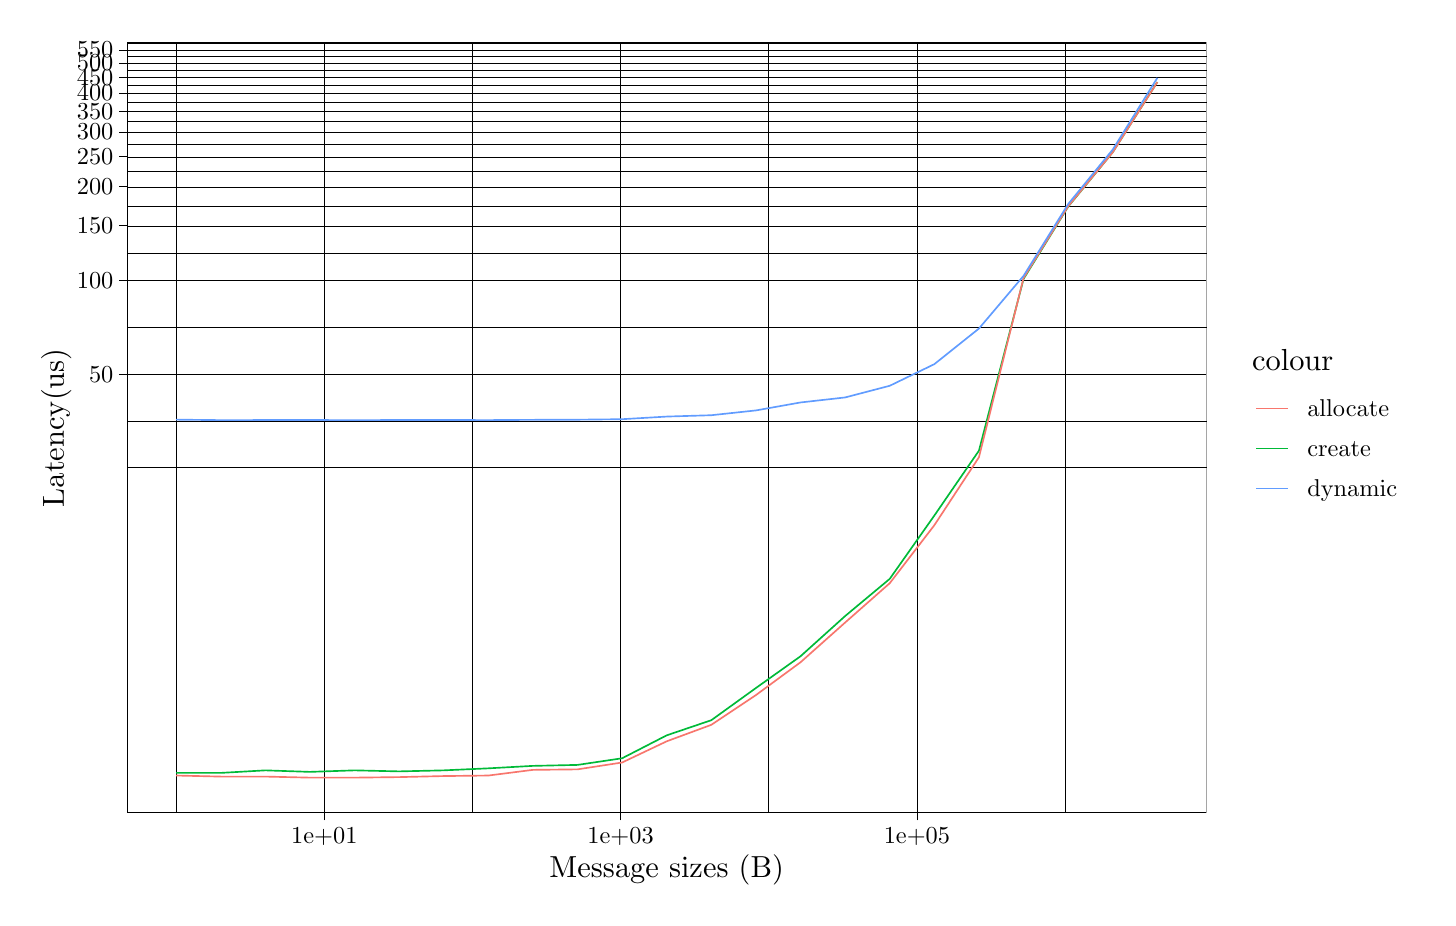
\begin{tikzpicture}[x=1pt,y=1pt]
\definecolor{fillColor}{RGB}{255,255,255}
\path[use as bounding box,fill=fillColor,fill opacity=0.00] (0,0) rectangle (505.89,314.37);
\begin{scope}
\path[clip] (  0.00,  0.00) rectangle (505.89,314.37);
\definecolor{drawColor}{RGB}{255,255,255}
\definecolor{fillColor}{RGB}{255,255,255}

\path[draw=drawColor,line width= 0.6pt,line join=round,line cap=round,fill=fillColor] (  0.00,  0.00) rectangle (505.89,314.37);
\end{scope}
\begin{scope}
\path[clip] ( 35.92, 30.72) rectangle (425.93,308.87);
\definecolor{fillColor}{RGB}{255,255,255}

\path[fill=fillColor] ( 35.92, 30.72) rectangle (425.93,308.87);
\definecolor{drawColor}{RGB}{0,0,0}

\path[draw=drawColor,line width= 0.0pt,line join=round] ( 35.92,155.27) --
	(425.93,155.27);

\path[draw=drawColor,line width= 0.0pt,line join=round] ( 35.92,172.20) --
	(425.93,172.20);

\path[draw=drawColor,line width= 0.0pt,line join=round] ( 35.92,206.06) --
	(425.93,206.06);

\path[draw=drawColor,line width= 0.0pt,line join=round] ( 35.92,232.89) --
	(425.93,232.89);

\path[draw=drawColor,line width= 0.0pt,line join=round] ( 35.92,249.82) --
	(425.93,249.82);

\path[draw=drawColor,line width= 0.0pt,line join=round] ( 35.92,262.30) --
	(425.93,262.30);

\path[draw=drawColor,line width= 0.0pt,line join=round] ( 35.92,272.21) --
	(425.93,272.21);

\path[draw=drawColor,line width= 0.0pt,line join=round] ( 35.92,280.42) --
	(425.93,280.42);

\path[draw=drawColor,line width= 0.0pt,line join=round] ( 35.92,287.45) --
	(425.93,287.45);

\path[draw=drawColor,line width= 0.0pt,line join=round] ( 35.92,293.59) --
	(425.93,293.59);

\path[draw=drawColor,line width= 0.0pt,line join=round] ( 35.92,299.04) --
	(425.93,299.04);

\path[draw=drawColor,line width= 0.0pt,line join=round] ( 35.92,303.94) --
	(425.93,303.94);

\path[draw=drawColor,line width= 0.0pt,line join=round] ( 53.64, 30.72) --
	( 53.64,308.87);

\path[draw=drawColor,line width= 0.0pt,line join=round] (160.72, 30.72) --
	(160.72,308.87);

\path[draw=drawColor,line width= 0.0pt,line join=round] (267.79, 30.72) --
	(267.79,308.87);

\path[draw=drawColor,line width= 0.0pt,line join=round] (374.87, 30.72) --
	(374.87,308.87);

\path[draw=drawColor,line width= 0.1pt,line join=round] ( 35.92,189.13) --
	(425.93,189.13);

\path[draw=drawColor,line width= 0.1pt,line join=round] ( 35.92,222.99) --
	(425.93,222.99);

\path[draw=drawColor,line width= 0.1pt,line join=round] ( 35.92,242.80) --
	(425.93,242.80);

\path[draw=drawColor,line width= 0.1pt,line join=round] ( 35.92,256.85) --
	(425.93,256.85);

\path[draw=drawColor,line width= 0.1pt,line join=round] ( 35.92,267.75) --
	(425.93,267.75);

\path[draw=drawColor,line width= 0.1pt,line join=round] ( 35.92,276.66) --
	(425.93,276.66);

\path[draw=drawColor,line width= 0.1pt,line join=round] ( 35.92,284.19) --
	(425.93,284.19);

\path[draw=drawColor,line width= 0.1pt,line join=round] ( 35.92,290.71) --
	(425.93,290.71);

\path[draw=drawColor,line width= 0.1pt,line join=round] ( 35.92,296.47) --
	(425.93,296.47);

\path[draw=drawColor,line width= 0.1pt,line join=round] ( 35.92,301.61) --
	(425.93,301.61);

\path[draw=drawColor,line width= 0.1pt,line join=round] ( 35.92,306.27) --
	(425.93,306.27);

\path[draw=drawColor,line width= 0.1pt,line join=round] (107.18, 30.72) --
	(107.18,308.87);

\path[draw=drawColor,line width= 0.1pt,line join=round] (214.26, 30.72) --
	(214.26,308.87);

\path[draw=drawColor,line width= 0.1pt,line join=round] (321.33, 30.72) --
	(321.33,308.87);
\definecolor{drawColor}{RGB}{0,186,56}

\path[draw=drawColor,line width= 0.6pt,line join=round] ( 53.64, 45.08) --
	( 69.76, 45.08) --
	( 85.88, 46.00) --
	(101.99, 45.45) --
	(118.11, 46.00) --
	(134.23, 45.63) --
	(150.34, 46.00) --
	(166.46, 46.73) --
	(182.58, 47.62) --
	(198.69, 47.97) --
	(214.81, 50.37) --
	(230.92, 58.66) --
	(247.04, 64.13) --
	(263.16, 75.76) --
	(279.27, 87.23) --
	(295.39,101.76) --
	(311.51,115.21) --
	(327.62,138.07) --
	(343.74,161.52) --
	(359.86,223.59) --
	(375.97,249.68) --
	(392.09,269.35) --
	(408.20,294.73);
\definecolor{drawColor}{RGB}{248,118,109}

\path[draw=drawColor,line width= 0.6pt,line join=round] ( 53.64, 44.13) --
	( 69.76, 43.75) --
	( 85.88, 43.75) --
	(101.99, 43.37) --
	(118.11, 43.37) --
	(134.23, 43.56) --
	(150.34, 43.94) --
	(166.46, 44.13) --
	(182.58, 46.18) --
	(198.69, 46.36) --
	(214.81, 48.84) --
	(230.92, 56.50) --
	(247.04, 62.46) --
	(263.16, 73.21) --
	(279.27, 85.06) --
	(295.39, 99.42) --
	(311.51,113.63) --
	(327.62,134.58) --
	(343.74,159.14) --
	(359.86,223.92) --
	(375.97,249.81) --
	(392.09,269.34) --
	(408.20,294.69);
\definecolor{drawColor}{RGB}{97,156,255}

\path[draw=drawColor,line width= 0.6pt,line join=round] ( 53.64,172.73) --
	( 69.76,172.55) --
	( 85.88,172.58) --
	(101.99,172.58) --
	(118.11,172.56) --
	(134.23,172.58) --
	(150.34,172.60) --
	(166.46,172.56) --
	(182.58,172.66) --
	(198.69,172.71) --
	(214.81,172.89) --
	(230.92,173.84) --
	(247.04,174.33) --
	(263.16,176.06) --
	(279.27,178.94) --
	(295.39,180.75) --
	(311.51,184.97) --
	(327.62,192.78) --
	(343.74,205.65) --
	(359.86,224.69) --
	(375.97,250.62) --
	(392.09,270.33) --
	(408.20,296.23);
\definecolor{drawColor}{RGB}{0,0,0}

\path[draw=drawColor,line width= 0.6pt,line join=round,line cap=round] ( 35.92, 30.72) rectangle (425.93,308.87);
\end{scope}
\begin{scope}
\path[clip] (  0.00,  0.00) rectangle (505.89,314.37);
\definecolor{drawColor}{RGB}{0,0,0}

\node[text=drawColor,anchor=base west,inner sep=0pt, outer sep=0pt, scale=  0.88] at ( 22.17,186.31) {50};

\node[text=drawColor,anchor=base west,inner sep=0pt, outer sep=0pt, scale=  0.88] at ( 17.77,220.17) {100};

\node[text=drawColor,anchor=base west,inner sep=0pt, outer sep=0pt, scale=  0.88] at ( 17.77,239.98) {150};

\node[text=drawColor,anchor=base west,inner sep=0pt, outer sep=0pt, scale=  0.88] at ( 17.77,254.03) {200};

\node[text=drawColor,anchor=base west,inner sep=0pt, outer sep=0pt, scale=  0.88] at ( 17.77,264.93) {250};

\node[text=drawColor,anchor=base west,inner sep=0pt, outer sep=0pt, scale=  0.88] at ( 17.77,273.84) {300};

\node[text=drawColor,anchor=base west,inner sep=0pt, outer sep=0pt, scale=  0.88] at ( 17.77,281.37) {350};

\node[text=drawColor,anchor=base west,inner sep=0pt, outer sep=0pt, scale=  0.88] at ( 17.77,287.89) {400};

\node[text=drawColor,anchor=base west,inner sep=0pt, outer sep=0pt, scale=  0.88] at ( 17.77,293.64) {450};

\node[text=drawColor,anchor=base west,inner sep=0pt, outer sep=0pt, scale=  0.88] at ( 17.77,298.79) {500};

\node[text=drawColor,anchor=base west,inner sep=0pt, outer sep=0pt, scale=  0.88] at ( 17.77,303.45) {550};
\end{scope}
\begin{scope}
\path[clip] (  0.00,  0.00) rectangle (505.89,314.37);
\definecolor{drawColor}{RGB}{0,0,0}

\path[draw=drawColor,line width= 0.3pt,line join=round] ( 33.17,189.13) --
	( 35.92,189.13);

\path[draw=drawColor,line width= 0.3pt,line join=round] ( 33.17,222.99) --
	( 35.92,222.99);

\path[draw=drawColor,line width= 0.3pt,line join=round] ( 33.17,242.80) --
	( 35.92,242.80);

\path[draw=drawColor,line width= 0.3pt,line join=round] ( 33.17,256.85) --
	( 35.92,256.85);

\path[draw=drawColor,line width= 0.3pt,line join=round] ( 33.17,267.75) --
	( 35.92,267.75);

\path[draw=drawColor,line width= 0.3pt,line join=round] ( 33.17,276.66) --
	( 35.92,276.66);

\path[draw=drawColor,line width= 0.3pt,line join=round] ( 33.17,284.19) --
	( 35.92,284.19);

\path[draw=drawColor,line width= 0.3pt,line join=round] ( 33.17,290.71) --
	( 35.92,290.71);

\path[draw=drawColor,line width= 0.3pt,line join=round] ( 33.17,296.47) --
	( 35.92,296.47);

\path[draw=drawColor,line width= 0.3pt,line join=round] ( 33.17,301.61) --
	( 35.92,301.61);

\path[draw=drawColor,line width= 0.3pt,line join=round] ( 33.17,306.27) --
	( 35.92,306.27);
\end{scope}
\begin{scope}
\path[clip] (  0.00,  0.00) rectangle (505.89,314.37);
\definecolor{drawColor}{RGB}{0,0,0}

\path[draw=drawColor,line width= 0.3pt,line join=round] (107.18, 27.97) --
	(107.18, 30.72);

\path[draw=drawColor,line width= 0.3pt,line join=round] (214.26, 27.97) --
	(214.26, 30.72);

\path[draw=drawColor,line width= 0.3pt,line join=round] (321.33, 27.97) --
	(321.33, 30.72);
\end{scope}
\begin{scope}
\path[clip] (  0.00,  0.00) rectangle (505.89,314.37);
\definecolor{drawColor}{RGB}{0,0,0}

\node[text=drawColor,anchor=base,inner sep=0pt, outer sep=0pt, scale=  0.88] at (107.18, 19.71) {1e+01};

\node[text=drawColor,anchor=base,inner sep=0pt, outer sep=0pt, scale=  0.88] at (214.26, 19.71) {1e+03};

\node[text=drawColor,anchor=base,inner sep=0pt, outer sep=0pt, scale=  0.88] at (321.33, 19.71) {1e+05};
\end{scope}
\begin{scope}
\path[clip] (  0.00,  0.00) rectangle (505.89,314.37);
\definecolor{drawColor}{RGB}{0,0,0}

\node[text=drawColor,anchor=base,inner sep=0pt, outer sep=0pt, scale=  1.10] at (230.92,  7.44) {Message sizes (B)};
\end{scope}
\begin{scope}
\path[clip] (  0.00,  0.00) rectangle (505.89,314.37);
\definecolor{drawColor}{RGB}{0,0,0}

\node[text=drawColor,rotate= 90.00,anchor=base,inner sep=0pt, outer sep=0pt, scale=  1.10] at ( 13.08,169.80) {Latency(us)};
\end{scope}
\begin{scope}
\path[clip] (  0.00,  0.00) rectangle (505.89,314.37);
\definecolor{fillColor}{RGB}{255,255,255}

\path[fill=fillColor] (436.93,135.11) rectangle (500.39,204.49);
\end{scope}
\begin{scope}
\path[clip] (  0.00,  0.00) rectangle (505.89,314.37);
\definecolor{drawColor}{RGB}{0,0,0}

\node[text=drawColor,anchor=base west,inner sep=0pt, outer sep=0pt, scale=  1.10] at (442.43,190.44) {colour};
\end{scope}
\begin{scope}
\path[clip] (  0.00,  0.00) rectangle (505.89,314.37);
\definecolor{fillColor}{RGB}{255,255,255}

\path[fill=fillColor] (442.43,169.52) rectangle (456.89,183.97);
\end{scope}
\begin{scope}
\path[clip] (  0.00,  0.00) rectangle (505.89,314.37);
\definecolor{drawColor}{RGB}{248,118,109}

\path[draw=drawColor,line width= 0.6pt,line join=round] (443.88,176.74) -- (455.44,176.74);
\end{scope}
\begin{scope}
\path[clip] (  0.00,  0.00) rectangle (505.89,314.37);
\definecolor{drawColor}{RGB}{248,118,109}

\path[draw=drawColor,line width= 0.6pt,line join=round] (443.88,176.74) -- (455.44,176.74);
\end{scope}
\begin{scope}
\path[clip] (  0.00,  0.00) rectangle (505.89,314.37);
\definecolor{drawColor}{RGB}{248,118,109}

\path[draw=drawColor,line width= 0.6pt,line join=round] (443.88,176.74) -- (455.44,176.74);
\end{scope}
\begin{scope}
\path[clip] (  0.00,  0.00) rectangle (505.89,314.37);
\definecolor{fillColor}{RGB}{255,255,255}

\path[fill=fillColor] (442.43,155.06) rectangle (456.89,169.52);
\end{scope}
\begin{scope}
\path[clip] (  0.00,  0.00) rectangle (505.89,314.37);
\definecolor{drawColor}{RGB}{0,186,56}

\path[draw=drawColor,line width= 0.6pt,line join=round] (443.88,162.29) -- (455.44,162.29);
\end{scope}
\begin{scope}
\path[clip] (  0.00,  0.00) rectangle (505.89,314.37);
\definecolor{drawColor}{RGB}{0,186,56}

\path[draw=drawColor,line width= 0.6pt,line join=round] (443.88,162.29) -- (455.44,162.29);
\end{scope}
\begin{scope}
\path[clip] (  0.00,  0.00) rectangle (505.89,314.37);
\definecolor{drawColor}{RGB}{0,186,56}

\path[draw=drawColor,line width= 0.6pt,line join=round] (443.88,162.29) -- (455.44,162.29);
\end{scope}
\begin{scope}
\path[clip] (  0.00,  0.00) rectangle (505.89,314.37);
\definecolor{fillColor}{RGB}{255,255,255}

\path[fill=fillColor] (442.43,140.61) rectangle (456.89,155.06);
\end{scope}
\begin{scope}
\path[clip] (  0.00,  0.00) rectangle (505.89,314.37);
\definecolor{drawColor}{RGB}{97,156,255}

\path[draw=drawColor,line width= 0.6pt,line join=round] (443.88,147.84) -- (455.44,147.84);
\end{scope}
\begin{scope}
\path[clip] (  0.00,  0.00) rectangle (505.89,314.37);
\definecolor{drawColor}{RGB}{97,156,255}

\path[draw=drawColor,line width= 0.6pt,line join=round] (443.88,147.84) -- (455.44,147.84);
\end{scope}
\begin{scope}
\path[clip] (  0.00,  0.00) rectangle (505.89,314.37);
\definecolor{drawColor}{RGB}{97,156,255}

\path[draw=drawColor,line width= 0.6pt,line join=round] (443.88,147.84) -- (455.44,147.84);
\end{scope}
\begin{scope}
\path[clip] (  0.00,  0.00) rectangle (505.89,314.37);
\definecolor{drawColor}{RGB}{0,0,0}

\node[text=drawColor,anchor=base west,inner sep=0pt, outer sep=0pt, scale=  0.88] at (462.39,173.71) {allocate};
\end{scope}
\begin{scope}
\path[clip] (  0.00,  0.00) rectangle (505.89,314.37);
\definecolor{drawColor}{RGB}{0,0,0}

\node[text=drawColor,anchor=base west,inner sep=0pt, outer sep=0pt, scale=  0.88] at (462.39,159.26) {create};
\end{scope}
\begin{scope}
\path[clip] (  0.00,  0.00) rectangle (505.89,314.37);
\definecolor{drawColor}{RGB}{0,0,0}

\node[text=drawColor,anchor=base west,inner sep=0pt, outer sep=0pt, scale=  0.88] at (462.39,144.81) {dynamic};
\end{scope}
\end{tikzpicture}

	\caption{2 nodes, get latency, gpu-gpu, flush-local, window algorithm comparisons}
\end{figure}

\begin{figure}
	% Created by tikzDevice version 0.10.1 on 2020-02-15 16:04:59
% !TEX encoding = UTF-8 Unicode
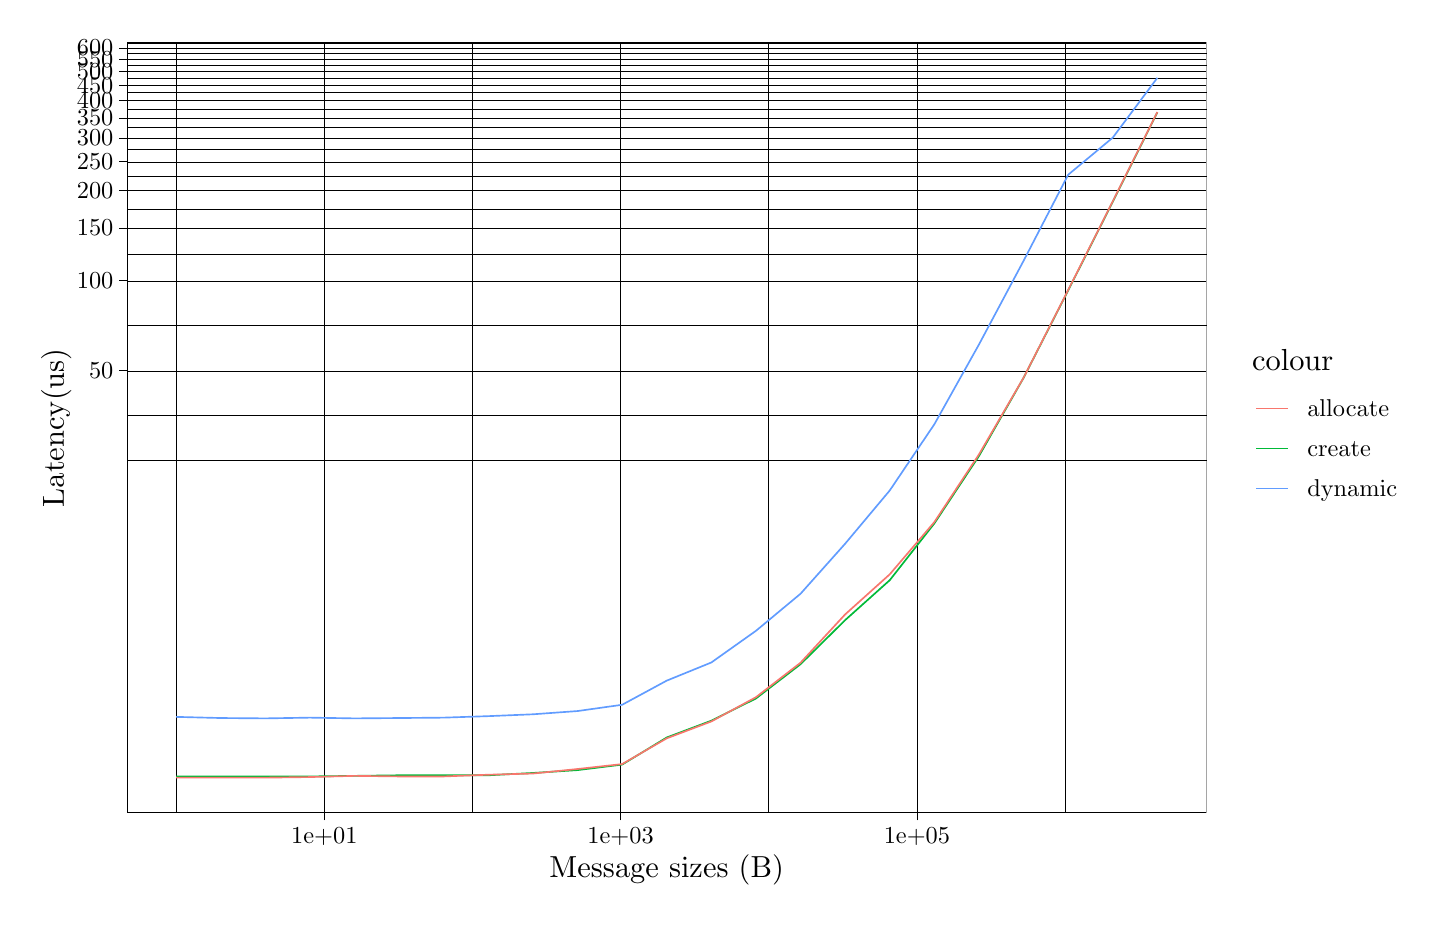
\begin{tikzpicture}[x=1pt,y=1pt]
\definecolor{fillColor}{RGB}{255,255,255}
\path[use as bounding box,fill=fillColor,fill opacity=0.00] (0,0) rectangle (505.89,314.37);
\begin{scope}
\path[clip] (  0.00,  0.00) rectangle (505.89,314.37);
\definecolor{drawColor}{RGB}{255,255,255}
\definecolor{fillColor}{RGB}{255,255,255}

\path[draw=drawColor,line width= 0.6pt,line join=round,line cap=round,fill=fillColor] (  0.00,  0.00) rectangle (505.89,314.37);
\end{scope}
\begin{scope}
\path[clip] ( 35.92, 30.72) rectangle (425.93,308.87);
\definecolor{fillColor}{RGB}{255,255,255}

\path[fill=fillColor] ( 35.92, 30.72) rectangle (425.93,308.87);
\definecolor{drawColor}{RGB}{0,0,0}

\path[draw=drawColor,line width= 0.0pt,line join=round] ( 35.92,157.87) --
	(425.93,157.87);

\path[draw=drawColor,line width= 0.0pt,line join=round] ( 35.92,174.14) --
	(425.93,174.14);

\path[draw=drawColor,line width= 0.0pt,line join=round] ( 35.92,206.68) --
	(425.93,206.68);

\path[draw=drawColor,line width= 0.0pt,line join=round] ( 35.92,232.46) --
	(425.93,232.46);

\path[draw=drawColor,line width= 0.0pt,line join=round] ( 35.92,248.73) --
	(425.93,248.73);

\path[draw=drawColor,line width= 0.0pt,line join=round] ( 35.92,260.71) --
	(425.93,260.71);

\path[draw=drawColor,line width= 0.0pt,line join=round] ( 35.92,270.23) --
	(425.93,270.23);

\path[draw=drawColor,line width= 0.0pt,line join=round] ( 35.92,278.13) --
	(425.93,278.13);

\path[draw=drawColor,line width= 0.0pt,line join=round] ( 35.92,284.88) --
	(425.93,284.88);

\path[draw=drawColor,line width= 0.0pt,line join=round] ( 35.92,290.78) --
	(425.93,290.78);

\path[draw=drawColor,line width= 0.0pt,line join=round] ( 35.92,296.01) --
	(425.93,296.01);

\path[draw=drawColor,line width= 0.0pt,line join=round] ( 35.92,300.72) --
	(425.93,300.72);

\path[draw=drawColor,line width= 0.0pt,line join=round] ( 35.92,305.00) --
	(425.93,305.00);

\path[draw=drawColor,line width= 0.0pt,line join=round] ( 53.64, 30.72) --
	( 53.64,308.87);

\path[draw=drawColor,line width= 0.0pt,line join=round] (160.72, 30.72) --
	(160.72,308.87);

\path[draw=drawColor,line width= 0.0pt,line join=round] (267.79, 30.72) --
	(267.79,308.87);

\path[draw=drawColor,line width= 0.0pt,line join=round] (374.87, 30.72) --
	(374.87,308.87);

\path[draw=drawColor,line width= 0.1pt,line join=round] ( 35.92,190.41) --
	(425.93,190.41);

\path[draw=drawColor,line width= 0.1pt,line join=round] ( 35.92,222.94) --
	(425.93,222.94);

\path[draw=drawColor,line width= 0.1pt,line join=round] ( 35.92,241.97) --
	(425.93,241.97);

\path[draw=drawColor,line width= 0.1pt,line join=round] ( 35.92,255.48) --
	(425.93,255.48);

\path[draw=drawColor,line width= 0.1pt,line join=round] ( 35.92,265.95) --
	(425.93,265.95);

\path[draw=drawColor,line width= 0.1pt,line join=round] ( 35.92,274.51) --
	(425.93,274.51);

\path[draw=drawColor,line width= 0.1pt,line join=round] ( 35.92,281.74) --
	(425.93,281.74);

\path[draw=drawColor,line width= 0.1pt,line join=round] ( 35.92,288.01) --
	(425.93,288.01);

\path[draw=drawColor,line width= 0.1pt,line join=round] ( 35.92,293.54) --
	(425.93,293.54);

\path[draw=drawColor,line width= 0.1pt,line join=round] ( 35.92,298.49) --
	(425.93,298.49);

\path[draw=drawColor,line width= 0.1pt,line join=round] ( 35.92,302.96) --
	(425.93,302.96);

\path[draw=drawColor,line width= 0.1pt,line join=round] ( 35.92,307.04) --
	(425.93,307.04);

\path[draw=drawColor,line width= 0.1pt,line join=round] (107.18, 30.72) --
	(107.18,308.87);

\path[draw=drawColor,line width= 0.1pt,line join=round] (214.26, 30.72) --
	(214.26,308.87);

\path[draw=drawColor,line width= 0.1pt,line join=round] (321.33, 30.72) --
	(321.33,308.87);
\definecolor{drawColor}{RGB}{0,186,56}

\path[draw=drawColor,line width= 0.6pt,line join=round] ( 53.64, 43.80) --
	( 69.76, 43.80) --
	( 85.88, 43.80) --
	(101.99, 43.80) --
	(118.11, 44.01) --
	(134.23, 44.22) --
	(150.34, 44.22) --
	(166.46, 44.22) --
	(182.58, 45.06) --
	(198.69, 46.09) --
	(214.81, 48.08) --
	(230.92, 57.88) --
	(247.04, 63.95) --
	(263.16, 71.97) --
	(279.27, 84.35) --
	(295.39,100.29) --
	(311.51,114.72) --
	(327.62,135.22) --
	(343.74,159.57) --
	(359.86,187.82) --
	(375.97,219.40) --
	(392.09,251.46) --
	(408.20,283.75);
\definecolor{drawColor}{RGB}{248,118,109}

\path[draw=drawColor,line width= 0.6pt,line join=round] ( 53.64, 43.37) --
	( 69.76, 43.37) --
	( 85.88, 43.37) --
	(101.99, 43.58) --
	(118.11, 44.01) --
	(134.23, 43.80) --
	(150.34, 43.80) --
	(166.46, 44.43) --
	(182.58, 44.85) --
	(198.69, 46.49) --
	(214.81, 48.27) --
	(230.92, 57.57) --
	(247.04, 63.67) --
	(263.16, 72.44) --
	(279.27, 84.89) --
	(295.39,102.35) --
	(311.51,116.84) --
	(327.62,135.71) --
	(343.74,160.16) --
	(359.86,187.88) --
	(375.97,219.56) --
	(392.09,251.61) --
	(408.20,283.90);
\definecolor{drawColor}{RGB}{97,156,255}

\path[draw=drawColor,line width= 0.6pt,line join=round] ( 53.64, 65.32) --
	( 69.76, 64.91) --
	( 85.88, 64.78) --
	(101.99, 65.05) --
	(118.11, 64.78) --
	(134.23, 64.91) --
	(150.34, 65.05) --
	(166.46, 65.59) --
	(182.58, 66.26) --
	(198.69, 67.43) --
	(214.81, 69.70) --
	(230.92, 78.42) --
	(247.04, 84.98) --
	(263.16, 96.42) --
	(279.27,109.82) --
	(295.39,127.90) --
	(311.51,147.14) --
	(327.62,171.05) --
	(343.74,199.87) --
	(359.86,230.11) --
	(375.97,261.21) --
	(392.09,274.63) --
	(408.20,296.23);
\definecolor{drawColor}{RGB}{0,0,0}

\path[draw=drawColor,line width= 0.6pt,line join=round,line cap=round] ( 35.92, 30.72) rectangle (425.93,308.87);
\end{scope}
\begin{scope}
\path[clip] (  0.00,  0.00) rectangle (505.89,314.37);
\definecolor{drawColor}{RGB}{0,0,0}

\node[text=drawColor,anchor=base west,inner sep=0pt, outer sep=0pt, scale=  0.88] at ( 22.17,187.59) {50};

\node[text=drawColor,anchor=base west,inner sep=0pt, outer sep=0pt, scale=  0.88] at ( 17.77,220.12) {100};

\node[text=drawColor,anchor=base west,inner sep=0pt, outer sep=0pt, scale=  0.88] at ( 17.77,239.15) {150};

\node[text=drawColor,anchor=base west,inner sep=0pt, outer sep=0pt, scale=  0.88] at ( 17.77,252.66) {200};

\node[text=drawColor,anchor=base west,inner sep=0pt, outer sep=0pt, scale=  0.88] at ( 17.77,263.13) {250};

\node[text=drawColor,anchor=base west,inner sep=0pt, outer sep=0pt, scale=  0.88] at ( 17.77,271.69) {300};

\node[text=drawColor,anchor=base west,inner sep=0pt, outer sep=0pt, scale=  0.88] at ( 17.77,278.92) {350};

\node[text=drawColor,anchor=base west,inner sep=0pt, outer sep=0pt, scale=  0.88] at ( 17.77,285.19) {400};

\node[text=drawColor,anchor=base west,inner sep=0pt, outer sep=0pt, scale=  0.88] at ( 17.77,290.72) {450};

\node[text=drawColor,anchor=base west,inner sep=0pt, outer sep=0pt, scale=  0.88] at ( 17.77,295.66) {500};

\node[text=drawColor,anchor=base west,inner sep=0pt, outer sep=0pt, scale=  0.88] at ( 17.77,300.14) {550};

\node[text=drawColor,anchor=base west,inner sep=0pt, outer sep=0pt, scale=  0.88] at ( 17.77,304.22) {600};
\end{scope}
\begin{scope}
\path[clip] (  0.00,  0.00) rectangle (505.89,314.37);
\definecolor{drawColor}{RGB}{0,0,0}

\path[draw=drawColor,line width= 0.3pt,line join=round] ( 33.17,190.41) --
	( 35.92,190.41);

\path[draw=drawColor,line width= 0.3pt,line join=round] ( 33.17,222.94) --
	( 35.92,222.94);

\path[draw=drawColor,line width= 0.3pt,line join=round] ( 33.17,241.97) --
	( 35.92,241.97);

\path[draw=drawColor,line width= 0.3pt,line join=round] ( 33.17,255.48) --
	( 35.92,255.48);

\path[draw=drawColor,line width= 0.3pt,line join=round] ( 33.17,265.95) --
	( 35.92,265.95);

\path[draw=drawColor,line width= 0.3pt,line join=round] ( 33.17,274.51) --
	( 35.92,274.51);

\path[draw=drawColor,line width= 0.3pt,line join=round] ( 33.17,281.74) --
	( 35.92,281.74);

\path[draw=drawColor,line width= 0.3pt,line join=round] ( 33.17,288.01) --
	( 35.92,288.01);

\path[draw=drawColor,line width= 0.3pt,line join=round] ( 33.17,293.54) --
	( 35.92,293.54);

\path[draw=drawColor,line width= 0.3pt,line join=round] ( 33.17,298.49) --
	( 35.92,298.49);

\path[draw=drawColor,line width= 0.3pt,line join=round] ( 33.17,302.96) --
	( 35.92,302.96);

\path[draw=drawColor,line width= 0.3pt,line join=round] ( 33.17,307.04) --
	( 35.92,307.04);
\end{scope}
\begin{scope}
\path[clip] (  0.00,  0.00) rectangle (505.89,314.37);
\definecolor{drawColor}{RGB}{0,0,0}

\path[draw=drawColor,line width= 0.3pt,line join=round] (107.18, 27.97) --
	(107.18, 30.72);

\path[draw=drawColor,line width= 0.3pt,line join=round] (214.26, 27.97) --
	(214.26, 30.72);

\path[draw=drawColor,line width= 0.3pt,line join=round] (321.33, 27.97) --
	(321.33, 30.72);
\end{scope}
\begin{scope}
\path[clip] (  0.00,  0.00) rectangle (505.89,314.37);
\definecolor{drawColor}{RGB}{0,0,0}

\node[text=drawColor,anchor=base,inner sep=0pt, outer sep=0pt, scale=  0.88] at (107.18, 19.71) {1e+01};

\node[text=drawColor,anchor=base,inner sep=0pt, outer sep=0pt, scale=  0.88] at (214.26, 19.71) {1e+03};

\node[text=drawColor,anchor=base,inner sep=0pt, outer sep=0pt, scale=  0.88] at (321.33, 19.71) {1e+05};
\end{scope}
\begin{scope}
\path[clip] (  0.00,  0.00) rectangle (505.89,314.37);
\definecolor{drawColor}{RGB}{0,0,0}

\node[text=drawColor,anchor=base,inner sep=0pt, outer sep=0pt, scale=  1.10] at (230.92,  7.44) {Message sizes (B)};
\end{scope}
\begin{scope}
\path[clip] (  0.00,  0.00) rectangle (505.89,314.37);
\definecolor{drawColor}{RGB}{0,0,0}

\node[text=drawColor,rotate= 90.00,anchor=base,inner sep=0pt, outer sep=0pt, scale=  1.10] at ( 13.08,169.80) {Latency(us)};
\end{scope}
\begin{scope}
\path[clip] (  0.00,  0.00) rectangle (505.89,314.37);
\definecolor{fillColor}{RGB}{255,255,255}

\path[fill=fillColor] (436.93,135.11) rectangle (500.39,204.49);
\end{scope}
\begin{scope}
\path[clip] (  0.00,  0.00) rectangle (505.89,314.37);
\definecolor{drawColor}{RGB}{0,0,0}

\node[text=drawColor,anchor=base west,inner sep=0pt, outer sep=0pt, scale=  1.10] at (442.43,190.44) {colour};
\end{scope}
\begin{scope}
\path[clip] (  0.00,  0.00) rectangle (505.89,314.37);
\definecolor{fillColor}{RGB}{255,255,255}

\path[fill=fillColor] (442.43,169.52) rectangle (456.89,183.97);
\end{scope}
\begin{scope}
\path[clip] (  0.00,  0.00) rectangle (505.89,314.37);
\definecolor{drawColor}{RGB}{248,118,109}

\path[draw=drawColor,line width= 0.6pt,line join=round] (443.88,176.74) -- (455.44,176.74);
\end{scope}
\begin{scope}
\path[clip] (  0.00,  0.00) rectangle (505.89,314.37);
\definecolor{drawColor}{RGB}{248,118,109}

\path[draw=drawColor,line width= 0.6pt,line join=round] (443.88,176.74) -- (455.44,176.74);
\end{scope}
\begin{scope}
\path[clip] (  0.00,  0.00) rectangle (505.89,314.37);
\definecolor{drawColor}{RGB}{248,118,109}

\path[draw=drawColor,line width= 0.6pt,line join=round] (443.88,176.74) -- (455.44,176.74);
\end{scope}
\begin{scope}
\path[clip] (  0.00,  0.00) rectangle (505.89,314.37);
\definecolor{fillColor}{RGB}{255,255,255}

\path[fill=fillColor] (442.43,155.06) rectangle (456.89,169.52);
\end{scope}
\begin{scope}
\path[clip] (  0.00,  0.00) rectangle (505.89,314.37);
\definecolor{drawColor}{RGB}{0,186,56}

\path[draw=drawColor,line width= 0.6pt,line join=round] (443.88,162.29) -- (455.44,162.29);
\end{scope}
\begin{scope}
\path[clip] (  0.00,  0.00) rectangle (505.89,314.37);
\definecolor{drawColor}{RGB}{0,186,56}

\path[draw=drawColor,line width= 0.6pt,line join=round] (443.88,162.29) -- (455.44,162.29);
\end{scope}
\begin{scope}
\path[clip] (  0.00,  0.00) rectangle (505.89,314.37);
\definecolor{drawColor}{RGB}{0,186,56}

\path[draw=drawColor,line width= 0.6pt,line join=round] (443.88,162.29) -- (455.44,162.29);
\end{scope}
\begin{scope}
\path[clip] (  0.00,  0.00) rectangle (505.89,314.37);
\definecolor{fillColor}{RGB}{255,255,255}

\path[fill=fillColor] (442.43,140.61) rectangle (456.89,155.06);
\end{scope}
\begin{scope}
\path[clip] (  0.00,  0.00) rectangle (505.89,314.37);
\definecolor{drawColor}{RGB}{97,156,255}

\path[draw=drawColor,line width= 0.6pt,line join=round] (443.88,147.84) -- (455.44,147.84);
\end{scope}
\begin{scope}
\path[clip] (  0.00,  0.00) rectangle (505.89,314.37);
\definecolor{drawColor}{RGB}{97,156,255}

\path[draw=drawColor,line width= 0.6pt,line join=round] (443.88,147.84) -- (455.44,147.84);
\end{scope}
\begin{scope}
\path[clip] (  0.00,  0.00) rectangle (505.89,314.37);
\definecolor{drawColor}{RGB}{97,156,255}

\path[draw=drawColor,line width= 0.6pt,line join=round] (443.88,147.84) -- (455.44,147.84);
\end{scope}
\begin{scope}
\path[clip] (  0.00,  0.00) rectangle (505.89,314.37);
\definecolor{drawColor}{RGB}{0,0,0}

\node[text=drawColor,anchor=base west,inner sep=0pt, outer sep=0pt, scale=  0.88] at (462.39,173.71) {allocate};
\end{scope}
\begin{scope}
\path[clip] (  0.00,  0.00) rectangle (505.89,314.37);
\definecolor{drawColor}{RGB}{0,0,0}

\node[text=drawColor,anchor=base west,inner sep=0pt, outer sep=0pt, scale=  0.88] at (462.39,159.26) {create};
\end{scope}
\begin{scope}
\path[clip] (  0.00,  0.00) rectangle (505.89,314.37);
\definecolor{drawColor}{RGB}{0,0,0}

\node[text=drawColor,anchor=base west,inner sep=0pt, outer sep=0pt, scale=  0.88] at (462.39,144.81) {dynamic};
\end{scope}
\end{tikzpicture}

	\caption{2 nodes, get latency, cpu-cpu, flush-local, window algorithm comparisons}
\end{figure}

\begin{figure}
	% Created by tikzDevice version 0.10.1 on 2020-02-15 16:05:40
% !TEX encoding = UTF-8 Unicode
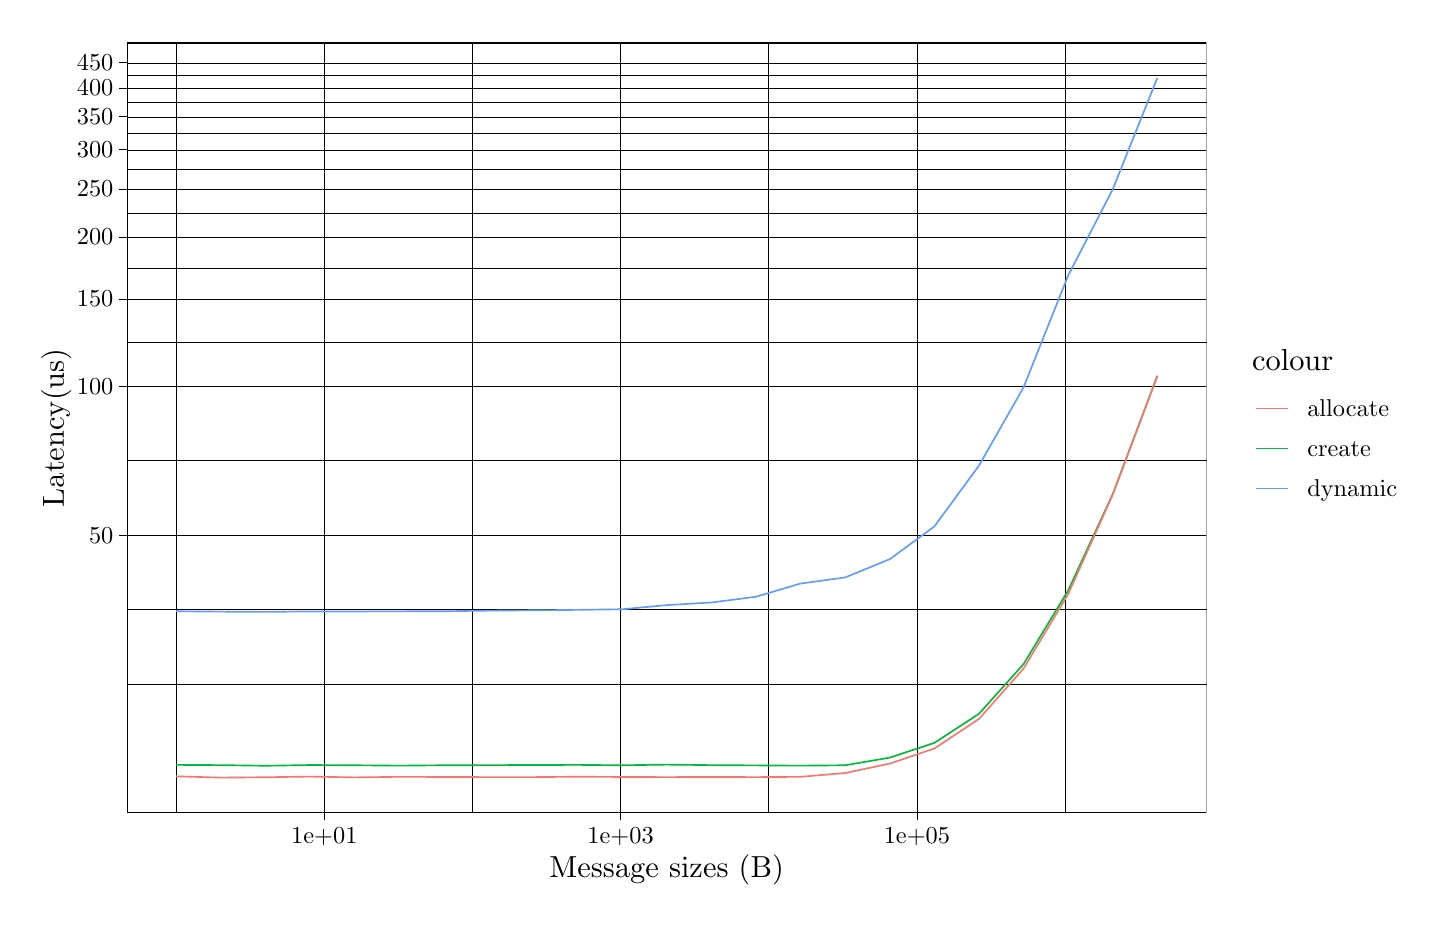
\begin{tikzpicture}[x=1pt,y=1pt]
\definecolor{fillColor}{RGB}{255,255,255}
\path[use as bounding box,fill=fillColor,fill opacity=0.00] (0,0) rectangle (505.89,314.37);
\begin{scope}
\path[clip] (  0.00,  0.00) rectangle (505.89,314.37);
\definecolor{drawColor}{RGB}{255,255,255}
\definecolor{fillColor}{RGB}{255,255,255}

\path[draw=drawColor,line width= 0.6pt,line join=round,line cap=round,fill=fillColor] (  0.00,  0.00) rectangle (505.89,314.37);
\end{scope}
\begin{scope}
\path[clip] ( 35.92, 30.72) rectangle (425.93,308.87);
\definecolor{fillColor}{RGB}{255,255,255}

\path[fill=fillColor] ( 35.92, 30.72) rectangle (425.93,308.87);
\definecolor{drawColor}{RGB}{0,0,0}

\path[draw=drawColor,line width= 0.0pt,line join=round] ( 35.92, 77.04) --
	(425.93, 77.04);

\path[draw=drawColor,line width= 0.0pt,line join=round] ( 35.92,103.98) --
	(425.93,103.98);

\path[draw=drawColor,line width= 0.0pt,line join=round] ( 35.92,157.86) --
	(425.93,157.86);

\path[draw=drawColor,line width= 0.0pt,line join=round] ( 35.92,200.56) --
	(425.93,200.56);

\path[draw=drawColor,line width= 0.0pt,line join=round] ( 35.92,227.50) --
	(425.93,227.50);

\path[draw=drawColor,line width= 0.0pt,line join=round] ( 35.92,247.35) --
	(425.93,247.35);

\path[draw=drawColor,line width= 0.0pt,line join=round] ( 35.92,263.11) --
	(425.93,263.11);

\path[draw=drawColor,line width= 0.0pt,line join=round] ( 35.92,276.19) --
	(425.93,276.19);

\path[draw=drawColor,line width= 0.0pt,line join=round] ( 35.92,287.37) --
	(425.93,287.37);

\path[draw=drawColor,line width= 0.0pt,line join=round] ( 35.92,297.14) --
	(425.93,297.14);

\path[draw=drawColor,line width= 0.0pt,line join=round] ( 53.64, 30.72) --
	( 53.64,308.87);

\path[draw=drawColor,line width= 0.0pt,line join=round] (160.72, 30.72) --
	(160.72,308.87);

\path[draw=drawColor,line width= 0.0pt,line join=round] (267.79, 30.72) --
	(267.79,308.87);

\path[draw=drawColor,line width= 0.0pt,line join=round] (374.87, 30.72) --
	(374.87,308.87);

\path[draw=drawColor,line width= 0.1pt,line join=round] ( 35.92,130.92) --
	(425.93,130.92);

\path[draw=drawColor,line width= 0.1pt,line join=round] ( 35.92,184.80) --
	(425.93,184.80);

\path[draw=drawColor,line width= 0.1pt,line join=round] ( 35.92,216.32) --
	(425.93,216.32);

\path[draw=drawColor,line width= 0.1pt,line join=round] ( 35.92,238.68) --
	(425.93,238.68);

\path[draw=drawColor,line width= 0.1pt,line join=round] ( 35.92,256.03) --
	(425.93,256.03);

\path[draw=drawColor,line width= 0.1pt,line join=round] ( 35.92,270.20) --
	(425.93,270.20);

\path[draw=drawColor,line width= 0.1pt,line join=round] ( 35.92,282.18) --
	(425.93,282.18);

\path[draw=drawColor,line width= 0.1pt,line join=round] ( 35.92,292.56) --
	(425.93,292.56);

\path[draw=drawColor,line width= 0.1pt,line join=round] ( 35.92,301.71) --
	(425.93,301.71);

\path[draw=drawColor,line width= 0.1pt,line join=round] (107.18, 30.72) --
	(107.18,308.87);

\path[draw=drawColor,line width= 0.1pt,line join=round] (214.26, 30.72) --
	(214.26,308.87);

\path[draw=drawColor,line width= 0.1pt,line join=round] (321.33, 30.72) --
	(321.33,308.87);
\definecolor{drawColor}{RGB}{0,186,56}

\path[draw=drawColor,line width= 0.6pt,line join=round] ( 53.64, 47.98) --
	( 69.76, 47.89) --
	( 85.88, 47.66) --
	(101.99, 47.93) --
	(118.11, 47.84) --
	(134.23, 47.70) --
	(150.34, 47.84) --
	(166.46, 47.89) --
	(182.58, 47.93) --
	(198.69, 47.98) --
	(214.81, 47.84) --
	(230.92, 48.07) --
	(247.04, 47.89) --
	(263.16, 47.79) --
	(279.27, 47.70) --
	(295.39, 47.84) --
	(311.51, 50.60) --
	(327.62, 55.92) --
	(343.74, 66.43) --
	(359.86, 84.40) --
	(375.97,110.99) --
	(392.09,145.83) --
	(408.20,188.58);
\definecolor{drawColor}{RGB}{248,118,109}

\path[draw=drawColor,line width= 0.6pt,line join=round] ( 53.64, 43.85) --
	( 69.76, 43.37) --
	( 85.88, 43.51) --
	(101.99, 43.75) --
	(118.11, 43.46) --
	(134.23, 43.66) --
	(150.34, 43.61) --
	(166.46, 43.56) --
	(182.58, 43.56) --
	(198.69, 43.70) --
	(214.81, 43.61) --
	(230.92, 43.56) --
	(247.04, 43.61) --
	(263.16, 43.56) --
	(279.27, 43.66) --
	(295.39, 45.03) --
	(311.51, 48.43) --
	(327.62, 53.89) --
	(343.74, 64.59) --
	(359.86, 82.80) --
	(375.97,109.65) --
	(392.09,145.66) --
	(408.20,188.48);
\definecolor{drawColor}{RGB}{97,156,255}

\path[draw=drawColor,line width= 0.6pt,line join=round] ( 53.64,103.49) --
	( 69.76,103.35) --
	( 85.88,103.27) --
	(101.99,103.42) --
	(118.11,103.42) --
	(134.23,103.46) --
	(150.34,103.49) --
	(166.46,103.71) --
	(182.58,103.84) --
	(198.69,103.99) --
	(214.81,104.21) --
	(230.92,105.71) --
	(247.04,106.65) --
	(263.16,108.73) --
	(279.27,113.50) --
	(295.39,115.71) --
	(311.51,122.30) --
	(327.62,134.12) --
	(343.74,156.11) --
	(359.86,184.39) --
	(375.97,224.81) --
	(392.09,255.98) --
	(408.20,296.23);
\definecolor{drawColor}{RGB}{0,0,0}

\path[draw=drawColor,line width= 0.6pt,line join=round,line cap=round] ( 35.92, 30.72) rectangle (425.93,308.87);
\end{scope}
\begin{scope}
\path[clip] (  0.00,  0.00) rectangle (505.89,314.37);
\definecolor{drawColor}{RGB}{0,0,0}

\node[text=drawColor,anchor=base west,inner sep=0pt, outer sep=0pt, scale=  0.88] at ( 22.17,128.10) {50};

\node[text=drawColor,anchor=base west,inner sep=0pt, outer sep=0pt, scale=  0.88] at ( 17.77,181.98) {100};

\node[text=drawColor,anchor=base west,inner sep=0pt, outer sep=0pt, scale=  0.88] at ( 17.77,213.50) {150};

\node[text=drawColor,anchor=base west,inner sep=0pt, outer sep=0pt, scale=  0.88] at ( 17.77,235.86) {200};

\node[text=drawColor,anchor=base west,inner sep=0pt, outer sep=0pt, scale=  0.88] at ( 17.77,253.20) {250};

\node[text=drawColor,anchor=base west,inner sep=0pt, outer sep=0pt, scale=  0.88] at ( 17.77,267.37) {300};

\node[text=drawColor,anchor=base west,inner sep=0pt, outer sep=0pt, scale=  0.88] at ( 17.77,279.36) {350};

\node[text=drawColor,anchor=base west,inner sep=0pt, outer sep=0pt, scale=  0.88] at ( 17.77,289.74) {400};

\node[text=drawColor,anchor=base west,inner sep=0pt, outer sep=0pt, scale=  0.88] at ( 17.77,298.89) {450};
\end{scope}
\begin{scope}
\path[clip] (  0.00,  0.00) rectangle (505.89,314.37);
\definecolor{drawColor}{RGB}{0,0,0}

\path[draw=drawColor,line width= 0.3pt,line join=round] ( 33.17,130.92) --
	( 35.92,130.92);

\path[draw=drawColor,line width= 0.3pt,line join=round] ( 33.17,184.80) --
	( 35.92,184.80);

\path[draw=drawColor,line width= 0.3pt,line join=round] ( 33.17,216.32) --
	( 35.92,216.32);

\path[draw=drawColor,line width= 0.3pt,line join=round] ( 33.17,238.68) --
	( 35.92,238.68);

\path[draw=drawColor,line width= 0.3pt,line join=round] ( 33.17,256.03) --
	( 35.92,256.03);

\path[draw=drawColor,line width= 0.3pt,line join=round] ( 33.17,270.20) --
	( 35.92,270.20);

\path[draw=drawColor,line width= 0.3pt,line join=round] ( 33.17,282.18) --
	( 35.92,282.18);

\path[draw=drawColor,line width= 0.3pt,line join=round] ( 33.17,292.56) --
	( 35.92,292.56);

\path[draw=drawColor,line width= 0.3pt,line join=round] ( 33.17,301.71) --
	( 35.92,301.71);
\end{scope}
\begin{scope}
\path[clip] (  0.00,  0.00) rectangle (505.89,314.37);
\definecolor{drawColor}{RGB}{0,0,0}

\path[draw=drawColor,line width= 0.3pt,line join=round] (107.18, 27.97) --
	(107.18, 30.72);

\path[draw=drawColor,line width= 0.3pt,line join=round] (214.26, 27.97) --
	(214.26, 30.72);

\path[draw=drawColor,line width= 0.3pt,line join=round] (321.33, 27.97) --
	(321.33, 30.72);
\end{scope}
\begin{scope}
\path[clip] (  0.00,  0.00) rectangle (505.89,314.37);
\definecolor{drawColor}{RGB}{0,0,0}

\node[text=drawColor,anchor=base,inner sep=0pt, outer sep=0pt, scale=  0.88] at (107.18, 19.71) {1e+01};

\node[text=drawColor,anchor=base,inner sep=0pt, outer sep=0pt, scale=  0.88] at (214.26, 19.71) {1e+03};

\node[text=drawColor,anchor=base,inner sep=0pt, outer sep=0pt, scale=  0.88] at (321.33, 19.71) {1e+05};
\end{scope}
\begin{scope}
\path[clip] (  0.00,  0.00) rectangle (505.89,314.37);
\definecolor{drawColor}{RGB}{0,0,0}

\node[text=drawColor,anchor=base,inner sep=0pt, outer sep=0pt, scale=  1.10] at (230.92,  7.44) {Message sizes (B)};
\end{scope}
\begin{scope}
\path[clip] (  0.00,  0.00) rectangle (505.89,314.37);
\definecolor{drawColor}{RGB}{0,0,0}

\node[text=drawColor,rotate= 90.00,anchor=base,inner sep=0pt, outer sep=0pt, scale=  1.10] at ( 13.08,169.80) {Latency(us)};
\end{scope}
\begin{scope}
\path[clip] (  0.00,  0.00) rectangle (505.89,314.37);
\definecolor{fillColor}{RGB}{255,255,255}

\path[fill=fillColor] (436.93,135.11) rectangle (500.39,204.49);
\end{scope}
\begin{scope}
\path[clip] (  0.00,  0.00) rectangle (505.89,314.37);
\definecolor{drawColor}{RGB}{0,0,0}

\node[text=drawColor,anchor=base west,inner sep=0pt, outer sep=0pt, scale=  1.10] at (442.43,190.44) {colour};
\end{scope}
\begin{scope}
\path[clip] (  0.00,  0.00) rectangle (505.89,314.37);
\definecolor{fillColor}{RGB}{255,255,255}

\path[fill=fillColor] (442.43,169.52) rectangle (456.89,183.97);
\end{scope}
\begin{scope}
\path[clip] (  0.00,  0.00) rectangle (505.89,314.37);
\definecolor{drawColor}{RGB}{248,118,109}

\path[draw=drawColor,line width= 0.6pt,line join=round] (443.88,176.74) -- (455.44,176.74);
\end{scope}
\begin{scope}
\path[clip] (  0.00,  0.00) rectangle (505.89,314.37);
\definecolor{drawColor}{RGB}{248,118,109}

\path[draw=drawColor,line width= 0.6pt,line join=round] (443.88,176.74) -- (455.44,176.74);
\end{scope}
\begin{scope}
\path[clip] (  0.00,  0.00) rectangle (505.89,314.37);
\definecolor{drawColor}{RGB}{248,118,109}

\path[draw=drawColor,line width= 0.6pt,line join=round] (443.88,176.74) -- (455.44,176.74);
\end{scope}
\begin{scope}
\path[clip] (  0.00,  0.00) rectangle (505.89,314.37);
\definecolor{fillColor}{RGB}{255,255,255}

\path[fill=fillColor] (442.43,155.06) rectangle (456.89,169.52);
\end{scope}
\begin{scope}
\path[clip] (  0.00,  0.00) rectangle (505.89,314.37);
\definecolor{drawColor}{RGB}{0,186,56}

\path[draw=drawColor,line width= 0.6pt,line join=round] (443.88,162.29) -- (455.44,162.29);
\end{scope}
\begin{scope}
\path[clip] (  0.00,  0.00) rectangle (505.89,314.37);
\definecolor{drawColor}{RGB}{0,186,56}

\path[draw=drawColor,line width= 0.6pt,line join=round] (443.88,162.29) -- (455.44,162.29);
\end{scope}
\begin{scope}
\path[clip] (  0.00,  0.00) rectangle (505.89,314.37);
\definecolor{drawColor}{RGB}{0,186,56}

\path[draw=drawColor,line width= 0.6pt,line join=round] (443.88,162.29) -- (455.44,162.29);
\end{scope}
\begin{scope}
\path[clip] (  0.00,  0.00) rectangle (505.89,314.37);
\definecolor{fillColor}{RGB}{255,255,255}

\path[fill=fillColor] (442.43,140.61) rectangle (456.89,155.06);
\end{scope}
\begin{scope}
\path[clip] (  0.00,  0.00) rectangle (505.89,314.37);
\definecolor{drawColor}{RGB}{97,156,255}

\path[draw=drawColor,line width= 0.6pt,line join=round] (443.88,147.84) -- (455.44,147.84);
\end{scope}
\begin{scope}
\path[clip] (  0.00,  0.00) rectangle (505.89,314.37);
\definecolor{drawColor}{RGB}{97,156,255}

\path[draw=drawColor,line width= 0.6pt,line join=round] (443.88,147.84) -- (455.44,147.84);
\end{scope}
\begin{scope}
\path[clip] (  0.00,  0.00) rectangle (505.89,314.37);
\definecolor{drawColor}{RGB}{97,156,255}

\path[draw=drawColor,line width= 0.6pt,line join=round] (443.88,147.84) -- (455.44,147.84);
\end{scope}
\begin{scope}
\path[clip] (  0.00,  0.00) rectangle (505.89,314.37);
\definecolor{drawColor}{RGB}{0,0,0}

\node[text=drawColor,anchor=base west,inner sep=0pt, outer sep=0pt, scale=  0.88] at (462.39,173.71) {allocate};
\end{scope}
\begin{scope}
\path[clip] (  0.00,  0.00) rectangle (505.89,314.37);
\definecolor{drawColor}{RGB}{0,0,0}

\node[text=drawColor,anchor=base west,inner sep=0pt, outer sep=0pt, scale=  0.88] at (462.39,159.26) {create};
\end{scope}
\begin{scope}
\path[clip] (  0.00,  0.00) rectangle (505.89,314.37);
\definecolor{drawColor}{RGB}{0,0,0}

\node[text=drawColor,anchor=base west,inner sep=0pt, outer sep=0pt, scale=  0.88] at (462.39,144.81) {dynamic};
\end{scope}
\end{tikzpicture}

	\caption{1 node, get latency, gpu-gpu, flush-local, window algorithm comparisons}
\end{figure}

\begin{figure}
	% Created by tikzDevice version 0.10.1 on 2020-02-15 16:04:44
% !TEX encoding = UTF-8 Unicode
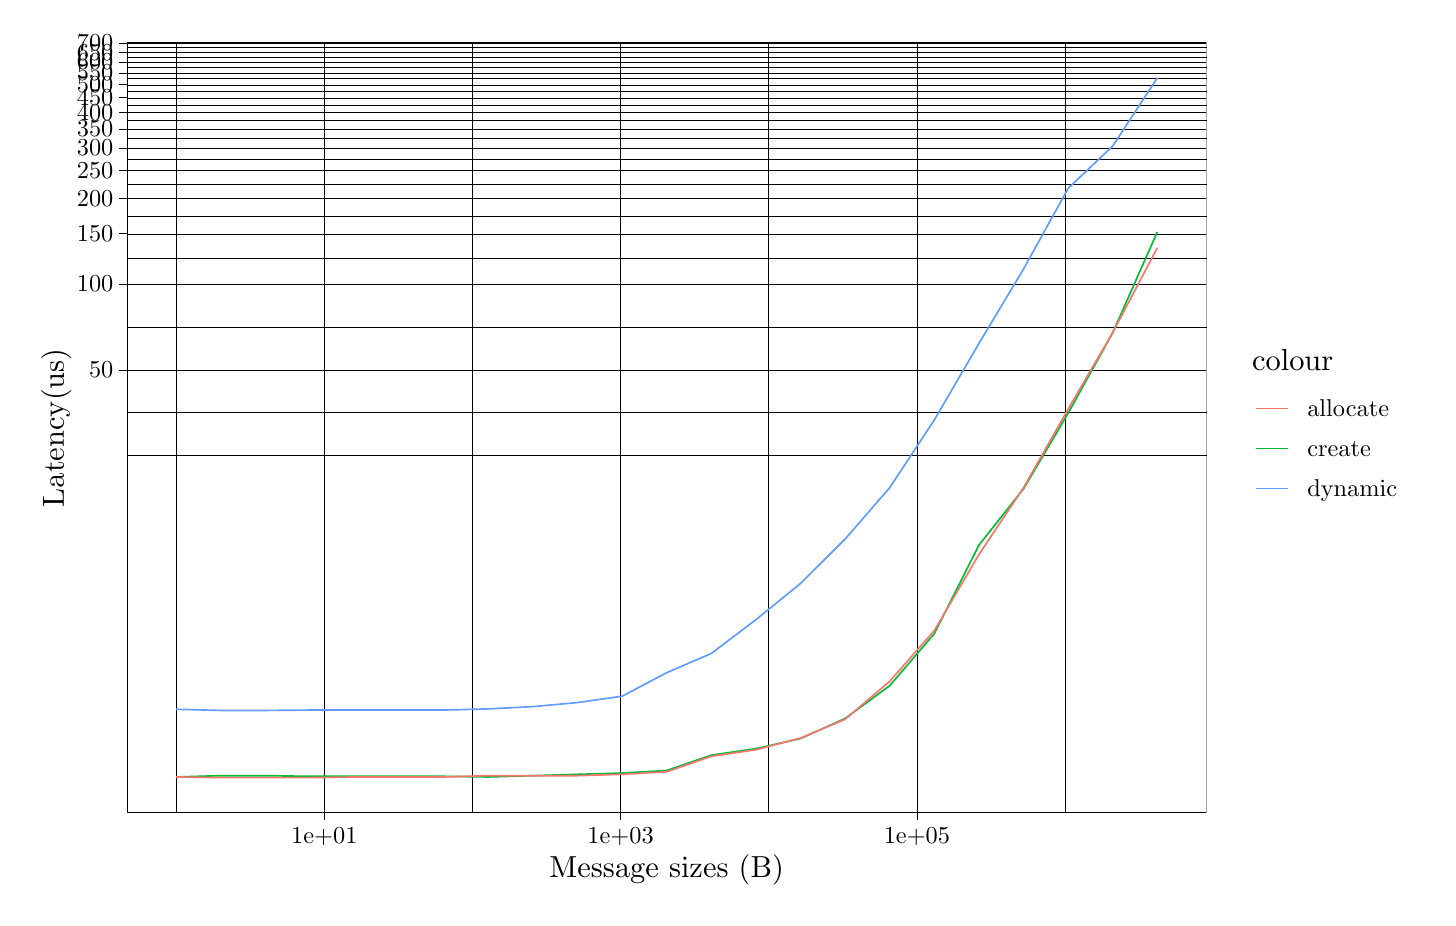
\begin{tikzpicture}[x=1pt,y=1pt]
\definecolor{fillColor}{RGB}{255,255,255}
\path[use as bounding box,fill=fillColor,fill opacity=0.00] (0,0) rectangle (505.89,314.37);
\begin{scope}
\path[clip] (  0.00,  0.00) rectangle (505.89,314.37);
\definecolor{drawColor}{RGB}{255,255,255}
\definecolor{fillColor}{RGB}{255,255,255}

\path[draw=drawColor,line width= 0.6pt,line join=round,line cap=round,fill=fillColor] (  0.00,  0.00) rectangle (505.89,314.37);
\end{scope}
\begin{scope}
\path[clip] ( 35.92, 30.72) rectangle (425.93,308.87);
\definecolor{fillColor}{RGB}{255,255,255}

\path[fill=fillColor] ( 35.92, 30.72) rectangle (425.93,308.87);
\definecolor{drawColor}{RGB}{0,0,0}

\path[draw=drawColor,line width= 0.0pt,line join=round] ( 35.92,159.66) --
	(425.93,159.66);

\path[draw=drawColor,line width= 0.0pt,line join=round] ( 35.92,175.17) --
	(425.93,175.17);

\path[draw=drawColor,line width= 0.0pt,line join=round] ( 35.92,206.20) --
	(425.93,206.20);

\path[draw=drawColor,line width= 0.0pt,line join=round] ( 35.92,230.78) --
	(425.93,230.78);

\path[draw=drawColor,line width= 0.0pt,line join=round] ( 35.92,246.29) --
	(425.93,246.29);

\path[draw=drawColor,line width= 0.0pt,line join=round] ( 35.92,257.72) --
	(425.93,257.72);

\path[draw=drawColor,line width= 0.0pt,line join=round] ( 35.92,266.80) --
	(425.93,266.80);

\path[draw=drawColor,line width= 0.0pt,line join=round] ( 35.92,274.33) --
	(425.93,274.33);

\path[draw=drawColor,line width= 0.0pt,line join=round] ( 35.92,280.77) --
	(425.93,280.77);

\path[draw=drawColor,line width= 0.0pt,line join=round] ( 35.92,286.39) --
	(425.93,286.39);

\path[draw=drawColor,line width= 0.0pt,line join=round] ( 35.92,291.38) --
	(425.93,291.38);

\path[draw=drawColor,line width= 0.0pt,line join=round] ( 35.92,295.87) --
	(425.93,295.87);

\path[draw=drawColor,line width= 0.0pt,line join=round] ( 35.92,299.95) --
	(425.93,299.95);

\path[draw=drawColor,line width= 0.0pt,line join=round] ( 35.92,303.69) --
	(425.93,303.69);

\path[draw=drawColor,line width= 0.0pt,line join=round] ( 35.92,307.14) --
	(425.93,307.14);

\path[draw=drawColor,line width= 0.0pt,line join=round] ( 53.64, 30.72) --
	( 53.64,308.87);

\path[draw=drawColor,line width= 0.0pt,line join=round] (160.72, 30.72) --
	(160.72,308.87);

\path[draw=drawColor,line width= 0.0pt,line join=round] (267.79, 30.72) --
	(267.79,308.87);

\path[draw=drawColor,line width= 0.0pt,line join=round] (374.87, 30.72) --
	(374.87,308.87);

\path[draw=drawColor,line width= 0.1pt,line join=round] ( 35.92,190.68) --
	(425.93,190.68);

\path[draw=drawColor,line width= 0.1pt,line join=round] ( 35.92,221.71) --
	(425.93,221.71);

\path[draw=drawColor,line width= 0.1pt,line join=round] ( 35.92,239.85) --
	(425.93,239.85);

\path[draw=drawColor,line width= 0.1pt,line join=round] ( 35.92,252.73) --
	(425.93,252.73);

\path[draw=drawColor,line width= 0.1pt,line join=round] ( 35.92,262.72) --
	(425.93,262.72);

\path[draw=drawColor,line width= 0.1pt,line join=round] ( 35.92,270.88) --
	(425.93,270.88);

\path[draw=drawColor,line width= 0.1pt,line join=round] ( 35.92,277.78) --
	(425.93,277.78);

\path[draw=drawColor,line width= 0.1pt,line join=round] ( 35.92,283.75) --
	(425.93,283.75);

\path[draw=drawColor,line width= 0.1pt,line join=round] ( 35.92,289.03) --
	(425.93,289.03);

\path[draw=drawColor,line width= 0.1pt,line join=round] ( 35.92,293.74) --
	(425.93,293.74);

\path[draw=drawColor,line width= 0.1pt,line join=round] ( 35.92,298.01) --
	(425.93,298.01);

\path[draw=drawColor,line width= 0.1pt,line join=round] ( 35.92,301.90) --
	(425.93,301.90);

\path[draw=drawColor,line width= 0.1pt,line join=round] ( 35.92,305.48) --
	(425.93,305.48);

\path[draw=drawColor,line width= 0.1pt,line join=round] ( 35.92,308.80) --
	(425.93,308.80);

\path[draw=drawColor,line width= 0.1pt,line join=round] (107.18, 30.72) --
	(107.18,308.87);

\path[draw=drawColor,line width= 0.1pt,line join=round] (214.26, 30.72) --
	(214.26,308.87);

\path[draw=drawColor,line width= 0.1pt,line join=round] (321.33, 30.72) --
	(321.33,308.87);
\definecolor{drawColor}{RGB}{0,186,56}

\path[draw=drawColor,line width= 0.6pt,line join=round] ( 53.64, 43.61) --
	( 69.76, 44.08) --
	( 85.88, 44.08) --
	(101.99, 43.85) --
	(118.11, 43.85) --
	(134.23, 43.85) --
	(150.34, 43.85) --
	(166.46, 43.61) --
	(182.58, 44.08) --
	(198.69, 44.56) --
	(214.81, 45.02) --
	(230.92, 45.94) --
	(247.04, 51.49) --
	(263.16, 53.83) --
	(279.27, 57.49) --
	(295.39, 64.76) --
	(311.51, 76.62) --
	(327.62, 95.41) --
	(343.74,127.40) --
	(359.86,147.75) --
	(375.97,175.08) --
	(392.09,204.17) --
	(408.20,240.59);
\definecolor{drawColor}{RGB}{248,118,109}

\path[draw=drawColor,line width= 0.6pt,line join=round] ( 53.64, 43.61) --
	( 69.76, 43.37) --
	( 85.88, 43.37) --
	(101.99, 43.37) --
	(118.11, 43.61) --
	(134.23, 43.61) --
	(150.34, 43.61) --
	(166.46, 44.08) --
	(182.58, 44.08) --
	(198.69, 44.08) --
	(214.81, 44.56) --
	(230.92, 45.48) --
	(247.04, 51.08) --
	(263.16, 53.45) --
	(279.27, 57.66) --
	(295.39, 64.46) --
	(311.51, 78.20) --
	(327.62, 96.53) --
	(343.74,124.00) --
	(359.86,148.17) --
	(375.97,176.55) --
	(392.09,204.24) --
	(408.20,234.84);
\definecolor{drawColor}{RGB}{97,156,255}

\path[draw=drawColor,line width= 0.6pt,line join=round] ( 53.64, 68.07) --
	( 69.76, 67.65) --
	( 85.88, 67.65) --
	(101.99, 67.79) --
	(118.11, 67.79) --
	(134.23, 67.79) --
	(150.34, 67.79) --
	(166.46, 68.21) --
	(182.58, 69.03) --
	(198.69, 70.50) --
	(214.81, 72.80) --
	(230.92, 81.29) --
	(247.04, 88.25) --
	(263.16,100.46) --
	(279.27,113.53) --
	(295.39,129.59) --
	(311.51,148.17) --
	(327.62,172.64) --
	(343.74,200.28) --
	(359.86,227.17) --
	(375.97,256.30) --
	(392.09,271.61) --
	(408.20,296.23);
\definecolor{drawColor}{RGB}{0,0,0}

\path[draw=drawColor,line width= 0.6pt,line join=round,line cap=round] ( 35.92, 30.72) rectangle (425.93,308.87);
\end{scope}
\begin{scope}
\path[clip] (  0.00,  0.00) rectangle (505.89,314.37);
\definecolor{drawColor}{RGB}{0,0,0}

\node[text=drawColor,anchor=base west,inner sep=0pt, outer sep=0pt, scale=  0.88] at ( 22.17,187.86) {50};

\node[text=drawColor,anchor=base west,inner sep=0pt, outer sep=0pt, scale=  0.88] at ( 17.77,218.88) {100};

\node[text=drawColor,anchor=base west,inner sep=0pt, outer sep=0pt, scale=  0.88] at ( 17.77,237.03) {150};

\node[text=drawColor,anchor=base west,inner sep=0pt, outer sep=0pt, scale=  0.88] at ( 17.77,249.91) {200};

\node[text=drawColor,anchor=base west,inner sep=0pt, outer sep=0pt, scale=  0.88] at ( 17.77,259.89) {250};

\node[text=drawColor,anchor=base west,inner sep=0pt, outer sep=0pt, scale=  0.88] at ( 17.77,268.06) {300};

\node[text=drawColor,anchor=base west,inner sep=0pt, outer sep=0pt, scale=  0.88] at ( 17.77,274.95) {350};

\node[text=drawColor,anchor=base west,inner sep=0pt, outer sep=0pt, scale=  0.88] at ( 17.77,280.93) {400};

\node[text=drawColor,anchor=base west,inner sep=0pt, outer sep=0pt, scale=  0.88] at ( 17.77,286.20) {450};

\node[text=drawColor,anchor=base west,inner sep=0pt, outer sep=0pt, scale=  0.88] at ( 17.77,290.92) {500};

\node[text=drawColor,anchor=base west,inner sep=0pt, outer sep=0pt, scale=  0.88] at ( 17.77,295.18) {550};

\node[text=drawColor,anchor=base west,inner sep=0pt, outer sep=0pt, scale=  0.88] at ( 17.77,299.08) {600};

\node[text=drawColor,anchor=base west,inner sep=0pt, outer sep=0pt, scale=  0.88] at ( 17.77,302.66) {650};

\node[text=drawColor,anchor=base west,inner sep=0pt, outer sep=0pt, scale=  0.88] at ( 17.77,305.98) {700};
\end{scope}
\begin{scope}
\path[clip] (  0.00,  0.00) rectangle (505.89,314.37);
\definecolor{drawColor}{RGB}{0,0,0}

\path[draw=drawColor,line width= 0.3pt,line join=round] ( 33.17,190.68) --
	( 35.92,190.68);

\path[draw=drawColor,line width= 0.3pt,line join=round] ( 33.17,221.71) --
	( 35.92,221.71);

\path[draw=drawColor,line width= 0.3pt,line join=round] ( 33.17,239.85) --
	( 35.92,239.85);

\path[draw=drawColor,line width= 0.3pt,line join=round] ( 33.17,252.73) --
	( 35.92,252.73);

\path[draw=drawColor,line width= 0.3pt,line join=round] ( 33.17,262.72) --
	( 35.92,262.72);

\path[draw=drawColor,line width= 0.3pt,line join=round] ( 33.17,270.88) --
	( 35.92,270.88);

\path[draw=drawColor,line width= 0.3pt,line join=round] ( 33.17,277.78) --
	( 35.92,277.78);

\path[draw=drawColor,line width= 0.3pt,line join=round] ( 33.17,283.75) --
	( 35.92,283.75);

\path[draw=drawColor,line width= 0.3pt,line join=round] ( 33.17,289.03) --
	( 35.92,289.03);

\path[draw=drawColor,line width= 0.3pt,line join=round] ( 33.17,293.74) --
	( 35.92,293.74);

\path[draw=drawColor,line width= 0.3pt,line join=round] ( 33.17,298.01) --
	( 35.92,298.01);

\path[draw=drawColor,line width= 0.3pt,line join=round] ( 33.17,301.90) --
	( 35.92,301.90);

\path[draw=drawColor,line width= 0.3pt,line join=round] ( 33.17,305.48) --
	( 35.92,305.48);

\path[draw=drawColor,line width= 0.3pt,line join=round] ( 33.17,308.80) --
	( 35.92,308.80);
\end{scope}
\begin{scope}
\path[clip] (  0.00,  0.00) rectangle (505.89,314.37);
\definecolor{drawColor}{RGB}{0,0,0}

\path[draw=drawColor,line width= 0.3pt,line join=round] (107.18, 27.97) --
	(107.18, 30.72);

\path[draw=drawColor,line width= 0.3pt,line join=round] (214.26, 27.97) --
	(214.26, 30.72);

\path[draw=drawColor,line width= 0.3pt,line join=round] (321.33, 27.97) --
	(321.33, 30.72);
\end{scope}
\begin{scope}
\path[clip] (  0.00,  0.00) rectangle (505.89,314.37);
\definecolor{drawColor}{RGB}{0,0,0}

\node[text=drawColor,anchor=base,inner sep=0pt, outer sep=0pt, scale=  0.88] at (107.18, 19.71) {1e+01};

\node[text=drawColor,anchor=base,inner sep=0pt, outer sep=0pt, scale=  0.88] at (214.26, 19.71) {1e+03};

\node[text=drawColor,anchor=base,inner sep=0pt, outer sep=0pt, scale=  0.88] at (321.33, 19.71) {1e+05};
\end{scope}
\begin{scope}
\path[clip] (  0.00,  0.00) rectangle (505.89,314.37);
\definecolor{drawColor}{RGB}{0,0,0}

\node[text=drawColor,anchor=base,inner sep=0pt, outer sep=0pt, scale=  1.10] at (230.92,  7.44) {Message sizes (B)};
\end{scope}
\begin{scope}
\path[clip] (  0.00,  0.00) rectangle (505.89,314.37);
\definecolor{drawColor}{RGB}{0,0,0}

\node[text=drawColor,rotate= 90.00,anchor=base,inner sep=0pt, outer sep=0pt, scale=  1.10] at ( 13.08,169.80) {Latency(us)};
\end{scope}
\begin{scope}
\path[clip] (  0.00,  0.00) rectangle (505.89,314.37);
\definecolor{fillColor}{RGB}{255,255,255}

\path[fill=fillColor] (436.93,135.11) rectangle (500.39,204.49);
\end{scope}
\begin{scope}
\path[clip] (  0.00,  0.00) rectangle (505.89,314.37);
\definecolor{drawColor}{RGB}{0,0,0}

\node[text=drawColor,anchor=base west,inner sep=0pt, outer sep=0pt, scale=  1.10] at (442.43,190.44) {colour};
\end{scope}
\begin{scope}
\path[clip] (  0.00,  0.00) rectangle (505.89,314.37);
\definecolor{fillColor}{RGB}{255,255,255}

\path[fill=fillColor] (442.43,169.52) rectangle (456.89,183.97);
\end{scope}
\begin{scope}
\path[clip] (  0.00,  0.00) rectangle (505.89,314.37);
\definecolor{drawColor}{RGB}{248,118,109}

\path[draw=drawColor,line width= 0.6pt,line join=round] (443.88,176.74) -- (455.44,176.74);
\end{scope}
\begin{scope}
\path[clip] (  0.00,  0.00) rectangle (505.89,314.37);
\definecolor{drawColor}{RGB}{248,118,109}

\path[draw=drawColor,line width= 0.6pt,line join=round] (443.88,176.74) -- (455.44,176.74);
\end{scope}
\begin{scope}
\path[clip] (  0.00,  0.00) rectangle (505.89,314.37);
\definecolor{drawColor}{RGB}{248,118,109}

\path[draw=drawColor,line width= 0.6pt,line join=round] (443.88,176.74) -- (455.44,176.74);
\end{scope}
\begin{scope}
\path[clip] (  0.00,  0.00) rectangle (505.89,314.37);
\definecolor{fillColor}{RGB}{255,255,255}

\path[fill=fillColor] (442.43,155.06) rectangle (456.89,169.52);
\end{scope}
\begin{scope}
\path[clip] (  0.00,  0.00) rectangle (505.89,314.37);
\definecolor{drawColor}{RGB}{0,186,56}

\path[draw=drawColor,line width= 0.6pt,line join=round] (443.88,162.29) -- (455.44,162.29);
\end{scope}
\begin{scope}
\path[clip] (  0.00,  0.00) rectangle (505.89,314.37);
\definecolor{drawColor}{RGB}{0,186,56}

\path[draw=drawColor,line width= 0.6pt,line join=round] (443.88,162.29) -- (455.44,162.29);
\end{scope}
\begin{scope}
\path[clip] (  0.00,  0.00) rectangle (505.89,314.37);
\definecolor{drawColor}{RGB}{0,186,56}

\path[draw=drawColor,line width= 0.6pt,line join=round] (443.88,162.29) -- (455.44,162.29);
\end{scope}
\begin{scope}
\path[clip] (  0.00,  0.00) rectangle (505.89,314.37);
\definecolor{fillColor}{RGB}{255,255,255}

\path[fill=fillColor] (442.43,140.61) rectangle (456.89,155.06);
\end{scope}
\begin{scope}
\path[clip] (  0.00,  0.00) rectangle (505.89,314.37);
\definecolor{drawColor}{RGB}{97,156,255}

\path[draw=drawColor,line width= 0.6pt,line join=round] (443.88,147.84) -- (455.44,147.84);
\end{scope}
\begin{scope}
\path[clip] (  0.00,  0.00) rectangle (505.89,314.37);
\definecolor{drawColor}{RGB}{97,156,255}

\path[draw=drawColor,line width= 0.6pt,line join=round] (443.88,147.84) -- (455.44,147.84);
\end{scope}
\begin{scope}
\path[clip] (  0.00,  0.00) rectangle (505.89,314.37);
\definecolor{drawColor}{RGB}{97,156,255}

\path[draw=drawColor,line width= 0.6pt,line join=round] (443.88,147.84) -- (455.44,147.84);
\end{scope}
\begin{scope}
\path[clip] (  0.00,  0.00) rectangle (505.89,314.37);
\definecolor{drawColor}{RGB}{0,0,0}

\node[text=drawColor,anchor=base west,inner sep=0pt, outer sep=0pt, scale=  0.88] at (462.39,173.71) {allocate};
\end{scope}
\begin{scope}
\path[clip] (  0.00,  0.00) rectangle (505.89,314.37);
\definecolor{drawColor}{RGB}{0,0,0}

\node[text=drawColor,anchor=base west,inner sep=0pt, outer sep=0pt, scale=  0.88] at (462.39,159.26) {create};
\end{scope}
\begin{scope}
\path[clip] (  0.00,  0.00) rectangle (505.89,314.37);
\definecolor{drawColor}{RGB}{0,0,0}

\node[text=drawColor,anchor=base west,inner sep=0pt, outer sep=0pt, scale=  0.88] at (462.39,144.81) {dynamic};
\end{scope}
\end{tikzpicture}

	\caption{1 node, get latency, cpu-cpu, flush-local, window algorithm comparisons}
\end{figure}

\begin{figure}
	% Created by tikzDevice version 0.10.1 on 2020-02-15 16:09:02
% !TEX encoding = UTF-8 Unicode
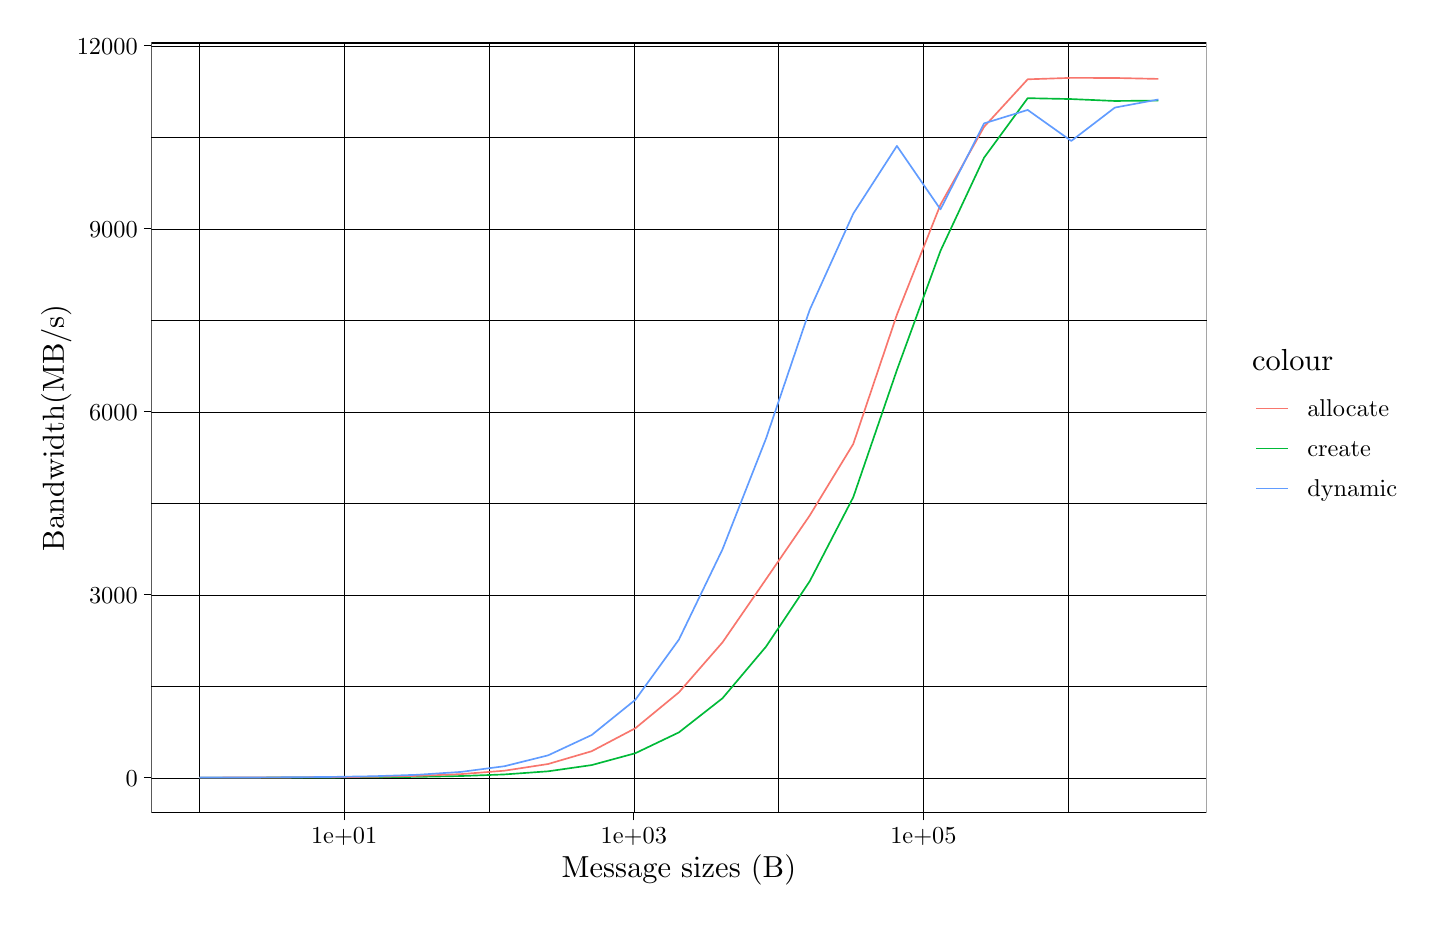
\begin{tikzpicture}[x=1pt,y=1pt]
\definecolor{fillColor}{RGB}{255,255,255}
\path[use as bounding box,fill=fillColor,fill opacity=0.00] (0,0) rectangle (505.89,314.37);
\begin{scope}
\path[clip] (  0.00,  0.00) rectangle (505.89,314.37);
\definecolor{drawColor}{RGB}{255,255,255}
\definecolor{fillColor}{RGB}{255,255,255}

\path[draw=drawColor,line width= 0.6pt,line join=round,line cap=round,fill=fillColor] (  0.00,  0.00) rectangle (505.89,314.37);
\end{scope}
\begin{scope}
\path[clip] ( 44.71, 30.72) rectangle (425.93,308.87);
\definecolor{fillColor}{RGB}{255,255,255}

\path[fill=fillColor] ( 44.71, 30.72) rectangle (425.93,308.87);
\definecolor{drawColor}{RGB}{0,0,0}

\path[draw=drawColor,line width= 0.0pt,line join=round] ( 44.71, 76.42) --
	(425.93, 76.42);

\path[draw=drawColor,line width= 0.0pt,line join=round] ( 44.71,142.55) --
	(425.93,142.55);

\path[draw=drawColor,line width= 0.0pt,line join=round] ( 44.71,208.67) --
	(425.93,208.67);

\path[draw=drawColor,line width= 0.0pt,line join=round] ( 44.71,274.80) --
	(425.93,274.80);

\path[draw=drawColor,line width= 0.0pt,line join=round] ( 62.04, 30.72) --
	( 62.04,308.87);

\path[draw=drawColor,line width= 0.0pt,line join=round] (166.70, 30.72) --
	(166.70,308.87);

\path[draw=drawColor,line width= 0.0pt,line join=round] (271.36, 30.72) --
	(271.36,308.87);

\path[draw=drawColor,line width= 0.0pt,line join=round] (376.02, 30.72) --
	(376.02,308.87);

\path[draw=drawColor,line width= 0.1pt,line join=round] ( 44.71, 43.36) --
	(425.93, 43.36);

\path[draw=drawColor,line width= 0.1pt,line join=round] ( 44.71,109.48) --
	(425.93,109.48);

\path[draw=drawColor,line width= 0.1pt,line join=round] ( 44.71,175.61) --
	(425.93,175.61);

\path[draw=drawColor,line width= 0.1pt,line join=round] ( 44.71,241.73) --
	(425.93,241.73);

\path[draw=drawColor,line width= 0.1pt,line join=round] ( 44.71,307.86) --
	(425.93,307.86);

\path[draw=drawColor,line width= 0.1pt,line join=round] (114.37, 30.72) --
	(114.37,308.87);

\path[draw=drawColor,line width= 0.1pt,line join=round] (219.03, 30.72) --
	(219.03,308.87);

\path[draw=drawColor,line width= 0.1pt,line join=round] (323.69, 30.72) --
	(323.69,308.87);
\definecolor{drawColor}{RGB}{0,186,56}

\path[draw=drawColor,line width= 0.6pt,line join=round] ( 62.04, 43.37) --
	( 77.80, 43.38) --
	( 93.55, 43.40) --
	(109.30, 43.43) --
	(125.05, 43.51) --
	(140.81, 43.65) --
	(156.56, 43.95) --
	(172.31, 44.53) --
	(188.07, 45.66) --
	(203.82, 47.91) --
	(219.57, 52.19) --
	(235.32, 59.72) --
	(251.08, 72.06) --
	(266.83, 90.74) --
	(282.58,114.31) --
	(298.33,144.72) --
	(314.09,190.64) --
	(329.84,233.73) --
	(345.59,267.39) --
	(361.35,288.89) --
	(377.10,288.57) --
	(392.85,287.88) --
	(408.60,288.02);
\definecolor{drawColor}{RGB}{248,118,109}

\path[draw=drawColor,line width= 0.6pt,line join=round] ( 62.04, 43.38) --
	( 77.80, 43.40) --
	( 93.55, 43.44) --
	(109.30, 43.52) --
	(125.05, 43.68) --
	(140.81, 44.00) --
	(156.56, 44.64) --
	(172.31, 45.88) --
	(188.07, 48.30) --
	(203.82, 52.92) --
	(219.57, 61.22) --
	(235.32, 74.18) --
	(251.08, 92.26) --
	(266.83,115.12) --
	(282.58,138.07) --
	(298.33,163.95) --
	(314.09,210.65) --
	(329.84,250.43) --
	(345.59,278.53) --
	(361.35,295.71) --
	(377.10,296.23) --
	(392.85,296.19) --
	(408.60,295.85);
\definecolor{drawColor}{RGB}{97,156,255}

\path[draw=drawColor,line width= 0.6pt,line join=round] ( 62.04, 43.39) --
	( 77.80, 43.42) --
	( 93.55, 43.49) --
	(109.30, 43.62) --
	(125.05, 43.88) --
	(140.81, 44.40) --
	(156.56, 45.44) --
	(172.31, 47.50) --
	(188.07, 51.43) --
	(203.82, 58.78) --
	(219.57, 71.49) --
	(235.32, 93.25) --
	(251.08,125.88) --
	(266.83,165.98) --
	(282.58,212.40) --
	(298.33,247.18) --
	(314.09,271.63) --
	(329.84,248.71) --
	(345.59,279.78) --
	(361.35,284.64) --
	(377.10,273.44) --
	(392.85,285.49) --
	(408.60,288.42);
\definecolor{drawColor}{RGB}{0,0,0}

\path[draw=drawColor,line width= 0.6pt,line join=round,line cap=round] ( 44.71, 30.72) rectangle (425.93,308.87);
\end{scope}
\begin{scope}
\path[clip] (  0.00,  0.00) rectangle (505.89,314.37);
\definecolor{drawColor}{RGB}{0,0,0}

\node[text=drawColor,anchor=base east,inner sep=0pt, outer sep=0pt, scale=  0.88] at ( 39.76, 40.33) {0};

\node[text=drawColor,anchor=base east,inner sep=0pt, outer sep=0pt, scale=  0.88] at ( 39.76,106.45) {3000};

\node[text=drawColor,anchor=base east,inner sep=0pt, outer sep=0pt, scale=  0.88] at ( 39.76,172.58) {6000};

\node[text=drawColor,anchor=base east,inner sep=0pt, outer sep=0pt, scale=  0.88] at ( 39.76,238.70) {9000};

\node[text=drawColor,anchor=base east,inner sep=0pt, outer sep=0pt, scale=  0.88] at ( 39.76,304.83) {12000};
\end{scope}
\begin{scope}
\path[clip] (  0.00,  0.00) rectangle (505.89,314.37);
\definecolor{drawColor}{RGB}{0,0,0}

\path[draw=drawColor,line width= 0.3pt,line join=round] ( 41.96, 43.36) --
	( 44.71, 43.36);

\path[draw=drawColor,line width= 0.3pt,line join=round] ( 41.96,109.48) --
	( 44.71,109.48);

\path[draw=drawColor,line width= 0.3pt,line join=round] ( 41.96,175.61) --
	( 44.71,175.61);

\path[draw=drawColor,line width= 0.3pt,line join=round] ( 41.96,241.73) --
	( 44.71,241.73);

\path[draw=drawColor,line width= 0.3pt,line join=round] ( 41.96,307.86) --
	( 44.71,307.86);
\end{scope}
\begin{scope}
\path[clip] (  0.00,  0.00) rectangle (505.89,314.37);
\definecolor{drawColor}{RGB}{0,0,0}

\path[draw=drawColor,line width= 0.3pt,line join=round] (114.37, 27.97) --
	(114.37, 30.72);

\path[draw=drawColor,line width= 0.3pt,line join=round] (219.03, 27.97) --
	(219.03, 30.72);

\path[draw=drawColor,line width= 0.3pt,line join=round] (323.69, 27.97) --
	(323.69, 30.72);
\end{scope}
\begin{scope}
\path[clip] (  0.00,  0.00) rectangle (505.89,314.37);
\definecolor{drawColor}{RGB}{0,0,0}

\node[text=drawColor,anchor=base,inner sep=0pt, outer sep=0pt, scale=  0.88] at (114.37, 19.71) {1e+01};

\node[text=drawColor,anchor=base,inner sep=0pt, outer sep=0pt, scale=  0.88] at (219.03, 19.71) {1e+03};

\node[text=drawColor,anchor=base,inner sep=0pt, outer sep=0pt, scale=  0.88] at (323.69, 19.71) {1e+05};
\end{scope}
\begin{scope}
\path[clip] (  0.00,  0.00) rectangle (505.89,314.37);
\definecolor{drawColor}{RGB}{0,0,0}

\node[text=drawColor,anchor=base,inner sep=0pt, outer sep=0pt, scale=  1.10] at (235.32,  7.44) {Message sizes (B)};
\end{scope}
\begin{scope}
\path[clip] (  0.00,  0.00) rectangle (505.89,314.37);
\definecolor{drawColor}{RGB}{0,0,0}

\node[text=drawColor,rotate= 90.00,anchor=base,inner sep=0pt, outer sep=0pt, scale=  1.10] at ( 13.08,169.80) {Bandwidth(MB/s)};
\end{scope}
\begin{scope}
\path[clip] (  0.00,  0.00) rectangle (505.89,314.37);
\definecolor{fillColor}{RGB}{255,255,255}

\path[fill=fillColor] (436.93,135.11) rectangle (500.39,204.49);
\end{scope}
\begin{scope}
\path[clip] (  0.00,  0.00) rectangle (505.89,314.37);
\definecolor{drawColor}{RGB}{0,0,0}

\node[text=drawColor,anchor=base west,inner sep=0pt, outer sep=0pt, scale=  1.10] at (442.43,190.44) {colour};
\end{scope}
\begin{scope}
\path[clip] (  0.00,  0.00) rectangle (505.89,314.37);
\definecolor{fillColor}{RGB}{255,255,255}

\path[fill=fillColor] (442.43,169.52) rectangle (456.89,183.97);
\end{scope}
\begin{scope}
\path[clip] (  0.00,  0.00) rectangle (505.89,314.37);
\definecolor{drawColor}{RGB}{248,118,109}

\path[draw=drawColor,line width= 0.6pt,line join=round] (443.88,176.74) -- (455.44,176.74);
\end{scope}
\begin{scope}
\path[clip] (  0.00,  0.00) rectangle (505.89,314.37);
\definecolor{drawColor}{RGB}{248,118,109}

\path[draw=drawColor,line width= 0.6pt,line join=round] (443.88,176.74) -- (455.44,176.74);
\end{scope}
\begin{scope}
\path[clip] (  0.00,  0.00) rectangle (505.89,314.37);
\definecolor{drawColor}{RGB}{248,118,109}

\path[draw=drawColor,line width= 0.6pt,line join=round] (443.88,176.74) -- (455.44,176.74);
\end{scope}
\begin{scope}
\path[clip] (  0.00,  0.00) rectangle (505.89,314.37);
\definecolor{fillColor}{RGB}{255,255,255}

\path[fill=fillColor] (442.43,155.06) rectangle (456.89,169.52);
\end{scope}
\begin{scope}
\path[clip] (  0.00,  0.00) rectangle (505.89,314.37);
\definecolor{drawColor}{RGB}{0,186,56}

\path[draw=drawColor,line width= 0.6pt,line join=round] (443.88,162.29) -- (455.44,162.29);
\end{scope}
\begin{scope}
\path[clip] (  0.00,  0.00) rectangle (505.89,314.37);
\definecolor{drawColor}{RGB}{0,186,56}

\path[draw=drawColor,line width= 0.6pt,line join=round] (443.88,162.29) -- (455.44,162.29);
\end{scope}
\begin{scope}
\path[clip] (  0.00,  0.00) rectangle (505.89,314.37);
\definecolor{drawColor}{RGB}{0,186,56}

\path[draw=drawColor,line width= 0.6pt,line join=round] (443.88,162.29) -- (455.44,162.29);
\end{scope}
\begin{scope}
\path[clip] (  0.00,  0.00) rectangle (505.89,314.37);
\definecolor{fillColor}{RGB}{255,255,255}

\path[fill=fillColor] (442.43,140.61) rectangle (456.89,155.06);
\end{scope}
\begin{scope}
\path[clip] (  0.00,  0.00) rectangle (505.89,314.37);
\definecolor{drawColor}{RGB}{97,156,255}

\path[draw=drawColor,line width= 0.6pt,line join=round] (443.88,147.84) -- (455.44,147.84);
\end{scope}
\begin{scope}
\path[clip] (  0.00,  0.00) rectangle (505.89,314.37);
\definecolor{drawColor}{RGB}{97,156,255}

\path[draw=drawColor,line width= 0.6pt,line join=round] (443.88,147.84) -- (455.44,147.84);
\end{scope}
\begin{scope}
\path[clip] (  0.00,  0.00) rectangle (505.89,314.37);
\definecolor{drawColor}{RGB}{97,156,255}

\path[draw=drawColor,line width= 0.6pt,line join=round] (443.88,147.84) -- (455.44,147.84);
\end{scope}
\begin{scope}
\path[clip] (  0.00,  0.00) rectangle (505.89,314.37);
\definecolor{drawColor}{RGB}{0,0,0}

\node[text=drawColor,anchor=base west,inner sep=0pt, outer sep=0pt, scale=  0.88] at (462.39,173.71) {allocate};
\end{scope}
\begin{scope}
\path[clip] (  0.00,  0.00) rectangle (505.89,314.37);
\definecolor{drawColor}{RGB}{0,0,0}

\node[text=drawColor,anchor=base west,inner sep=0pt, outer sep=0pt, scale=  0.88] at (462.39,159.26) {create};
\end{scope}
\begin{scope}
\path[clip] (  0.00,  0.00) rectangle (505.89,314.37);
\definecolor{drawColor}{RGB}{0,0,0}

\node[text=drawColor,anchor=base west,inner sep=0pt, outer sep=0pt, scale=  0.88] at (462.39,144.81) {dynamic};
\end{scope}
\end{tikzpicture}

	\caption{2 nodes, get bw, cpu-cpu, flush-local, window algorithm comparisons}
\end{figure}

\begin{figure}
	% Created by tikzDevice version 0.10.1 on 2020-02-15 16:08:33
% !TEX encoding = UTF-8 Unicode
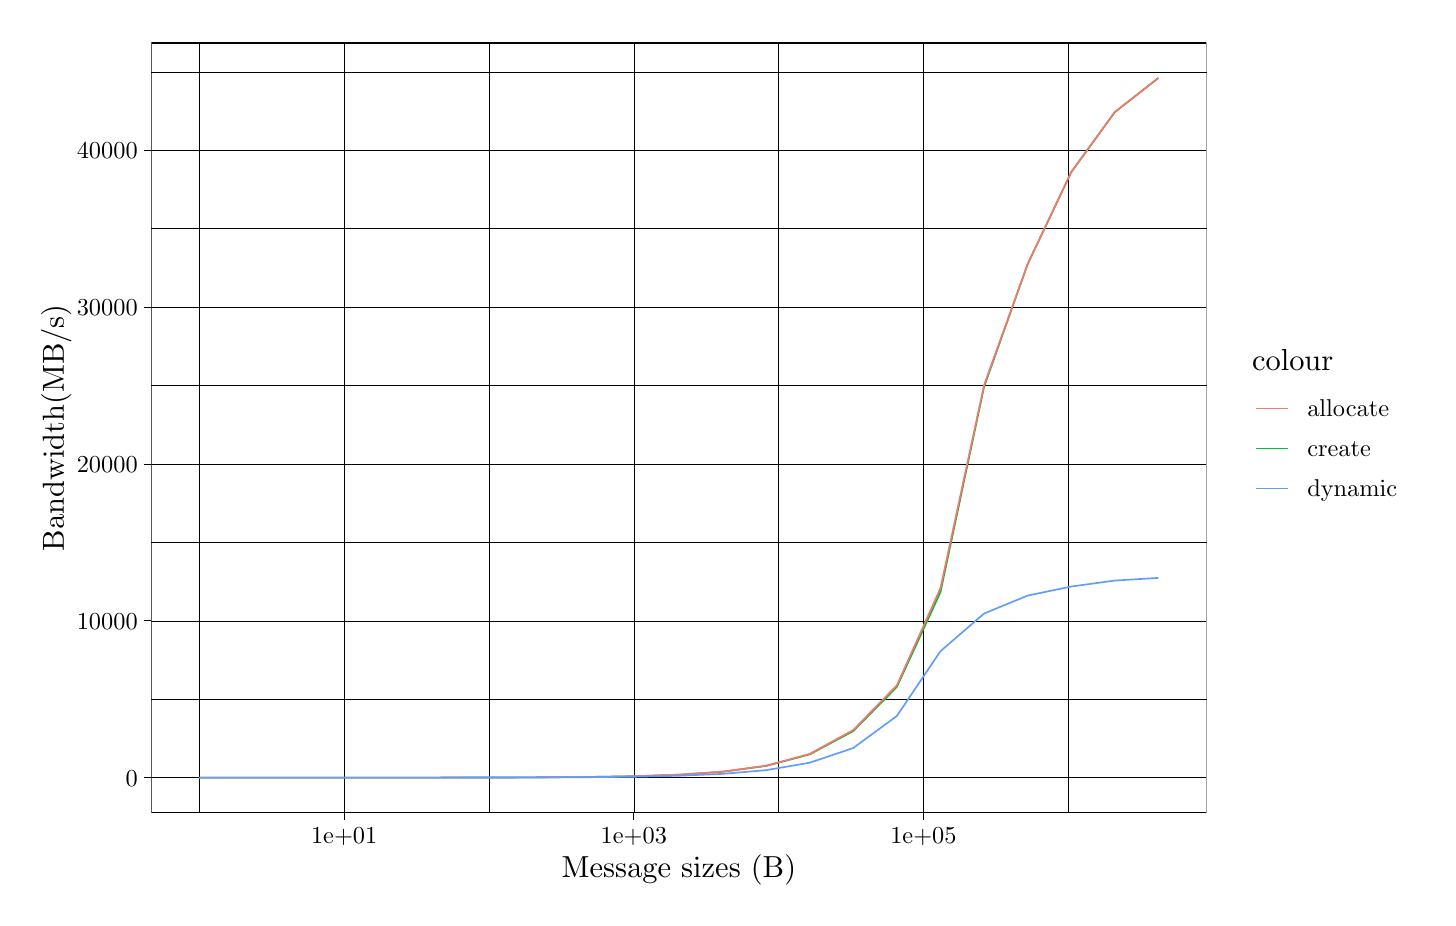
\begin{tikzpicture}[x=1pt,y=1pt]
\definecolor{fillColor}{RGB}{255,255,255}
\path[use as bounding box,fill=fillColor,fill opacity=0.00] (0,0) rectangle (505.89,314.37);
\begin{scope}
\path[clip] (  0.00,  0.00) rectangle (505.89,314.37);
\definecolor{drawColor}{RGB}{255,255,255}
\definecolor{fillColor}{RGB}{255,255,255}

\path[draw=drawColor,line width= 0.6pt,line join=round,line cap=round,fill=fillColor] (  0.00,  0.00) rectangle (505.89,314.37);
\end{scope}
\begin{scope}
\path[clip] ( 44.71, 30.72) rectangle (425.93,308.87);
\definecolor{fillColor}{RGB}{255,255,255}

\path[fill=fillColor] ( 44.71, 30.72) rectangle (425.93,308.87);
\definecolor{drawColor}{RGB}{0,0,0}

\path[draw=drawColor,line width= 0.0pt,line join=round] ( 44.71, 71.70) --
	(425.93, 71.70);

\path[draw=drawColor,line width= 0.0pt,line join=round] ( 44.71,128.35) --
	(425.93,128.35);

\path[draw=drawColor,line width= 0.0pt,line join=round] ( 44.71,185.01) --
	(425.93,185.01);

\path[draw=drawColor,line width= 0.0pt,line join=round] ( 44.71,241.67) --
	(425.93,241.67);

\path[draw=drawColor,line width= 0.0pt,line join=round] ( 44.71,298.32) --
	(425.93,298.32);

\path[draw=drawColor,line width= 0.0pt,line join=round] ( 62.04, 30.72) --
	( 62.04,308.87);

\path[draw=drawColor,line width= 0.0pt,line join=round] (166.70, 30.72) --
	(166.70,308.87);

\path[draw=drawColor,line width= 0.0pt,line join=round] (271.36, 30.72) --
	(271.36,308.87);

\path[draw=drawColor,line width= 0.0pt,line join=round] (376.02, 30.72) --
	(376.02,308.87);

\path[draw=drawColor,line width= 0.1pt,line join=round] ( 44.71, 43.37) --
	(425.93, 43.37);

\path[draw=drawColor,line width= 0.1pt,line join=round] ( 44.71,100.02) --
	(425.93,100.02);

\path[draw=drawColor,line width= 0.1pt,line join=round] ( 44.71,156.68) --
	(425.93,156.68);

\path[draw=drawColor,line width= 0.1pt,line join=round] ( 44.71,213.34) --
	(425.93,213.34);

\path[draw=drawColor,line width= 0.1pt,line join=round] ( 44.71,269.99) --
	(425.93,269.99);

\path[draw=drawColor,line width= 0.1pt,line join=round] (114.37, 30.72) --
	(114.37,308.87);

\path[draw=drawColor,line width= 0.1pt,line join=round] (219.03, 30.72) --
	(219.03,308.87);

\path[draw=drawColor,line width= 0.1pt,line join=round] (323.69, 30.72) --
	(323.69,308.87);
\definecolor{drawColor}{RGB}{0,186,56}

\path[draw=drawColor,line width= 0.6pt,line join=round] ( 62.04, 43.37) --
	( 77.80, 43.37) --
	( 93.55, 43.37) --
	(109.30, 43.37) --
	(125.05, 43.38) --
	(140.81, 43.38) --
	(156.56, 43.40) --
	(172.31, 43.43) --
	(188.07, 43.50) --
	(203.82, 43.63) --
	(219.57, 43.89) --
	(235.32, 44.42) --
	(251.08, 45.49) --
	(266.83, 47.59) --
	(282.58, 51.77) --
	(298.33, 60.20) --
	(314.09, 76.18) --
	(329.84,110.42) --
	(345.59,184.59) --
	(361.35,228.94) --
	(377.10,262.16) --
	(392.85,283.85) --
	(408.60,296.20);
\definecolor{drawColor}{RGB}{248,118,109}

\path[draw=drawColor,line width= 0.6pt,line join=round] ( 62.04, 43.37) --
	( 77.80, 43.37) --
	( 93.55, 43.37) --
	(109.30, 43.37) --
	(125.05, 43.38) --
	(140.81, 43.38) --
	(156.56, 43.40) --
	(172.31, 43.43) --
	(188.07, 43.50) --
	(203.82, 43.64) --
	(219.57, 43.90) --
	(235.32, 44.45) --
	(251.08, 45.53) --
	(266.83, 47.69) --
	(282.58, 51.94) --
	(298.33, 60.58) --
	(314.09, 76.74) --
	(329.84,111.87) --
	(345.59,185.19) --
	(361.35,229.02) --
	(377.10,262.25) --
	(392.85,283.92) --
	(408.60,296.23);
\definecolor{drawColor}{RGB}{97,156,255}

\path[draw=drawColor,line width= 0.6pt,line join=round] ( 62.04, 43.37) --
	( 77.80, 43.37) --
	( 93.55, 43.37) --
	(109.30, 43.37) --
	(125.05, 43.37) --
	(140.81, 43.38) --
	(156.56, 43.39) --
	(172.31, 43.41) --
	(188.07, 43.45) --
	(203.82, 43.54) --
	(219.57, 43.71) --
	(235.32, 44.05) --
	(251.08, 44.73) --
	(266.83, 46.07) --
	(282.58, 48.76) --
	(298.33, 54.08) --
	(314.09, 65.66) --
	(329.84, 89.07) --
	(345.59,102.67) --
	(361.35,109.15) --
	(377.10,112.43) --
	(392.85,114.58) --
	(408.60,115.55);
\definecolor{drawColor}{RGB}{0,0,0}

\path[draw=drawColor,line width= 0.6pt,line join=round,line cap=round] ( 44.71, 30.72) rectangle (425.93,308.87);
\end{scope}
\begin{scope}
\path[clip] (  0.00,  0.00) rectangle (505.89,314.37);
\definecolor{drawColor}{RGB}{0,0,0}

\node[text=drawColor,anchor=base east,inner sep=0pt, outer sep=0pt, scale=  0.88] at ( 39.76, 40.34) {0};

\node[text=drawColor,anchor=base east,inner sep=0pt, outer sep=0pt, scale=  0.88] at ( 39.76, 96.99) {10000};

\node[text=drawColor,anchor=base east,inner sep=0pt, outer sep=0pt, scale=  0.88] at ( 39.76,153.65) {20000};

\node[text=drawColor,anchor=base east,inner sep=0pt, outer sep=0pt, scale=  0.88] at ( 39.76,210.31) {30000};

\node[text=drawColor,anchor=base east,inner sep=0pt, outer sep=0pt, scale=  0.88] at ( 39.76,266.96) {40000};
\end{scope}
\begin{scope}
\path[clip] (  0.00,  0.00) rectangle (505.89,314.37);
\definecolor{drawColor}{RGB}{0,0,0}

\path[draw=drawColor,line width= 0.3pt,line join=round] ( 41.96, 43.37) --
	( 44.71, 43.37);

\path[draw=drawColor,line width= 0.3pt,line join=round] ( 41.96,100.02) --
	( 44.71,100.02);

\path[draw=drawColor,line width= 0.3pt,line join=round] ( 41.96,156.68) --
	( 44.71,156.68);

\path[draw=drawColor,line width= 0.3pt,line join=round] ( 41.96,213.34) --
	( 44.71,213.34);

\path[draw=drawColor,line width= 0.3pt,line join=round] ( 41.96,269.99) --
	( 44.71,269.99);
\end{scope}
\begin{scope}
\path[clip] (  0.00,  0.00) rectangle (505.89,314.37);
\definecolor{drawColor}{RGB}{0,0,0}

\path[draw=drawColor,line width= 0.3pt,line join=round] (114.37, 27.97) --
	(114.37, 30.72);

\path[draw=drawColor,line width= 0.3pt,line join=round] (219.03, 27.97) --
	(219.03, 30.72);

\path[draw=drawColor,line width= 0.3pt,line join=round] (323.69, 27.97) --
	(323.69, 30.72);
\end{scope}
\begin{scope}
\path[clip] (  0.00,  0.00) rectangle (505.89,314.37);
\definecolor{drawColor}{RGB}{0,0,0}

\node[text=drawColor,anchor=base,inner sep=0pt, outer sep=0pt, scale=  0.88] at (114.37, 19.71) {1e+01};

\node[text=drawColor,anchor=base,inner sep=0pt, outer sep=0pt, scale=  0.88] at (219.03, 19.71) {1e+03};

\node[text=drawColor,anchor=base,inner sep=0pt, outer sep=0pt, scale=  0.88] at (323.69, 19.71) {1e+05};
\end{scope}
\begin{scope}
\path[clip] (  0.00,  0.00) rectangle (505.89,314.37);
\definecolor{drawColor}{RGB}{0,0,0}

\node[text=drawColor,anchor=base,inner sep=0pt, outer sep=0pt, scale=  1.10] at (235.32,  7.44) {Message sizes (B)};
\end{scope}
\begin{scope}
\path[clip] (  0.00,  0.00) rectangle (505.89,314.37);
\definecolor{drawColor}{RGB}{0,0,0}

\node[text=drawColor,rotate= 90.00,anchor=base,inner sep=0pt, outer sep=0pt, scale=  1.10] at ( 13.08,169.80) {Bandwidth(MB/s)};
\end{scope}
\begin{scope}
\path[clip] (  0.00,  0.00) rectangle (505.89,314.37);
\definecolor{fillColor}{RGB}{255,255,255}

\path[fill=fillColor] (436.93,135.11) rectangle (500.39,204.49);
\end{scope}
\begin{scope}
\path[clip] (  0.00,  0.00) rectangle (505.89,314.37);
\definecolor{drawColor}{RGB}{0,0,0}

\node[text=drawColor,anchor=base west,inner sep=0pt, outer sep=0pt, scale=  1.10] at (442.43,190.44) {colour};
\end{scope}
\begin{scope}
\path[clip] (  0.00,  0.00) rectangle (505.89,314.37);
\definecolor{fillColor}{RGB}{255,255,255}

\path[fill=fillColor] (442.43,169.52) rectangle (456.89,183.97);
\end{scope}
\begin{scope}
\path[clip] (  0.00,  0.00) rectangle (505.89,314.37);
\definecolor{drawColor}{RGB}{248,118,109}

\path[draw=drawColor,line width= 0.6pt,line join=round] (443.88,176.74) -- (455.44,176.74);
\end{scope}
\begin{scope}
\path[clip] (  0.00,  0.00) rectangle (505.89,314.37);
\definecolor{drawColor}{RGB}{248,118,109}

\path[draw=drawColor,line width= 0.6pt,line join=round] (443.88,176.74) -- (455.44,176.74);
\end{scope}
\begin{scope}
\path[clip] (  0.00,  0.00) rectangle (505.89,314.37);
\definecolor{drawColor}{RGB}{248,118,109}

\path[draw=drawColor,line width= 0.6pt,line join=round] (443.88,176.74) -- (455.44,176.74);
\end{scope}
\begin{scope}
\path[clip] (  0.00,  0.00) rectangle (505.89,314.37);
\definecolor{fillColor}{RGB}{255,255,255}

\path[fill=fillColor] (442.43,155.06) rectangle (456.89,169.52);
\end{scope}
\begin{scope}
\path[clip] (  0.00,  0.00) rectangle (505.89,314.37);
\definecolor{drawColor}{RGB}{0,186,56}

\path[draw=drawColor,line width= 0.6pt,line join=round] (443.88,162.29) -- (455.44,162.29);
\end{scope}
\begin{scope}
\path[clip] (  0.00,  0.00) rectangle (505.89,314.37);
\definecolor{drawColor}{RGB}{0,186,56}

\path[draw=drawColor,line width= 0.6pt,line join=round] (443.88,162.29) -- (455.44,162.29);
\end{scope}
\begin{scope}
\path[clip] (  0.00,  0.00) rectangle (505.89,314.37);
\definecolor{drawColor}{RGB}{0,186,56}

\path[draw=drawColor,line width= 0.6pt,line join=round] (443.88,162.29) -- (455.44,162.29);
\end{scope}
\begin{scope}
\path[clip] (  0.00,  0.00) rectangle (505.89,314.37);
\definecolor{fillColor}{RGB}{255,255,255}

\path[fill=fillColor] (442.43,140.61) rectangle (456.89,155.06);
\end{scope}
\begin{scope}
\path[clip] (  0.00,  0.00) rectangle (505.89,314.37);
\definecolor{drawColor}{RGB}{97,156,255}

\path[draw=drawColor,line width= 0.6pt,line join=round] (443.88,147.84) -- (455.44,147.84);
\end{scope}
\begin{scope}
\path[clip] (  0.00,  0.00) rectangle (505.89,314.37);
\definecolor{drawColor}{RGB}{97,156,255}

\path[draw=drawColor,line width= 0.6pt,line join=round] (443.88,147.84) -- (455.44,147.84);
\end{scope}
\begin{scope}
\path[clip] (  0.00,  0.00) rectangle (505.89,314.37);
\definecolor{drawColor}{RGB}{97,156,255}

\path[draw=drawColor,line width= 0.6pt,line join=round] (443.88,147.84) -- (455.44,147.84);
\end{scope}
\begin{scope}
\path[clip] (  0.00,  0.00) rectangle (505.89,314.37);
\definecolor{drawColor}{RGB}{0,0,0}

\node[text=drawColor,anchor=base west,inner sep=0pt, outer sep=0pt, scale=  0.88] at (462.39,173.71) {allocate};
\end{scope}
\begin{scope}
\path[clip] (  0.00,  0.00) rectangle (505.89,314.37);
\definecolor{drawColor}{RGB}{0,0,0}

\node[text=drawColor,anchor=base west,inner sep=0pt, outer sep=0pt, scale=  0.88] at (462.39,159.26) {create};
\end{scope}
\begin{scope}
\path[clip] (  0.00,  0.00) rectangle (505.89,314.37);
\definecolor{drawColor}{RGB}{0,0,0}

\node[text=drawColor,anchor=base west,inner sep=0pt, outer sep=0pt, scale=  0.88] at (462.39,144.81) {dynamic};
\end{scope}
\end{tikzpicture}

	\caption{1 node, get bw, gpu-gpu, flush-local, window algorithm comparisons}
\end{figure}

\begin{figure}
	% Created by tikzDevice version 0.10.1 on 2020-02-15 16:08:50
% !TEX encoding = UTF-8 Unicode
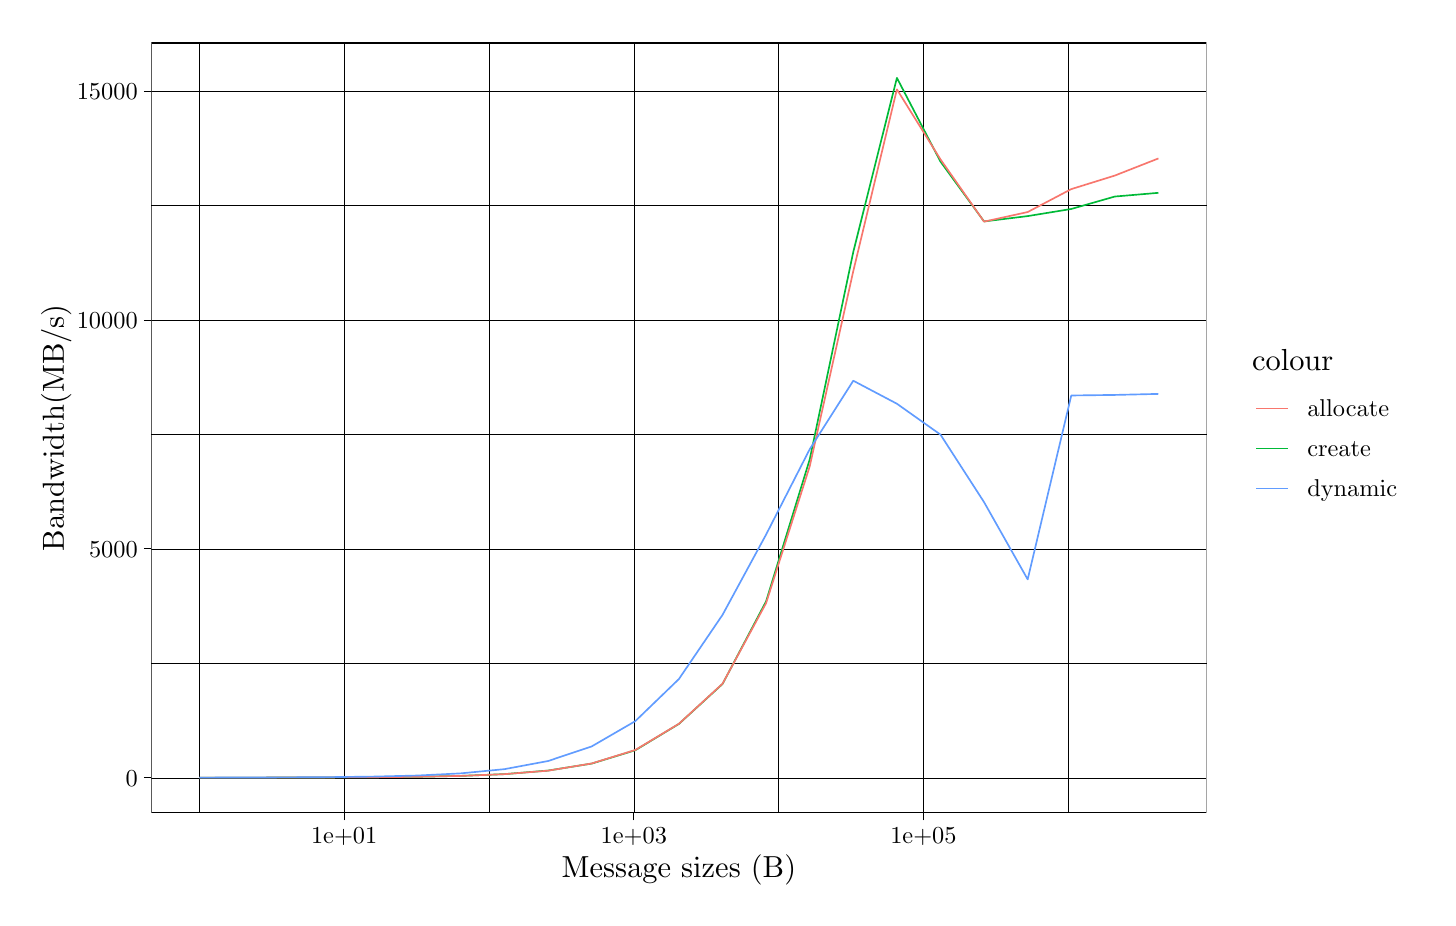
\begin{tikzpicture}[x=1pt,y=1pt]
\definecolor{fillColor}{RGB}{255,255,255}
\path[use as bounding box,fill=fillColor,fill opacity=0.00] (0,0) rectangle (505.89,314.37);
\begin{scope}
\path[clip] (  0.00,  0.00) rectangle (505.89,314.37);
\definecolor{drawColor}{RGB}{255,255,255}
\definecolor{fillColor}{RGB}{255,255,255}

\path[draw=drawColor,line width= 0.6pt,line join=round,line cap=round,fill=fillColor] (  0.00,  0.00) rectangle (505.89,314.37);
\end{scope}
\begin{scope}
\path[clip] ( 44.71, 30.72) rectangle (425.93,308.87);
\definecolor{fillColor}{RGB}{255,255,255}

\path[fill=fillColor] ( 44.71, 30.72) rectangle (425.93,308.87);
\definecolor{drawColor}{RGB}{0,0,0}

\path[draw=drawColor,line width= 0.0pt,line join=round] ( 44.71, 84.70) --
	(425.93, 84.70);

\path[draw=drawColor,line width= 0.0pt,line join=round] ( 44.71,167.39) --
	(425.93,167.39);

\path[draw=drawColor,line width= 0.0pt,line join=round] ( 44.71,250.08) --
	(425.93,250.08);

\path[draw=drawColor,line width= 0.0pt,line join=round] ( 62.04, 30.72) --
	( 62.04,308.87);

\path[draw=drawColor,line width= 0.0pt,line join=round] (166.70, 30.72) --
	(166.70,308.87);

\path[draw=drawColor,line width= 0.0pt,line join=round] (271.36, 30.72) --
	(271.36,308.87);

\path[draw=drawColor,line width= 0.0pt,line join=round] (376.02, 30.72) --
	(376.02,308.87);

\path[draw=drawColor,line width= 0.1pt,line join=round] ( 44.71, 43.36) --
	(425.93, 43.36);

\path[draw=drawColor,line width= 0.1pt,line join=round] ( 44.71,126.05) --
	(425.93,126.05);

\path[draw=drawColor,line width= 0.1pt,line join=round] ( 44.71,208.74) --
	(425.93,208.74);

\path[draw=drawColor,line width= 0.1pt,line join=round] ( 44.71,291.43) --
	(425.93,291.43);

\path[draw=drawColor,line width= 0.1pt,line join=round] (114.37, 30.72) --
	(114.37,308.87);

\path[draw=drawColor,line width= 0.1pt,line join=round] (219.03, 30.72) --
	(219.03,308.87);

\path[draw=drawColor,line width= 0.1pt,line join=round] (323.69, 30.72) --
	(323.69,308.87);
\definecolor{drawColor}{RGB}{0,186,56}

\path[draw=drawColor,line width= 0.6pt,line join=round] ( 62.04, 43.37) --
	( 77.80, 43.38) --
	( 93.55, 43.40) --
	(109.30, 43.44) --
	(125.05, 43.52) --
	(140.81, 43.68) --
	(156.56, 44.00) --
	(172.31, 44.64) --
	(188.07, 45.93) --
	(203.82, 48.45) --
	(219.57, 53.27) --
	(235.32, 62.78) --
	(251.08, 77.21) --
	(266.83,107.08) --
	(282.58,158.33) --
	(298.33,233.33) --
	(314.09,296.23) --
	(329.84,265.97) --
	(345.59,244.35) --
	(361.35,246.28) --
	(377.10,248.85) --
	(392.85,253.35) --
	(408.60,254.69);
\definecolor{drawColor}{RGB}{248,118,109}

\path[draw=drawColor,line width= 0.6pt,line join=round] ( 62.04, 43.37) --
	( 77.80, 43.38) --
	( 93.55, 43.40) --
	(109.30, 43.44) --
	(125.05, 43.52) --
	(140.81, 43.68) --
	(156.56, 44.00) --
	(172.31, 44.63) --
	(188.07, 45.89) --
	(203.82, 48.49) --
	(219.57, 53.37) --
	(235.32, 62.83) --
	(251.08, 77.30) --
	(266.83,106.45) --
	(282.58,155.83) --
	(298.33,226.39) --
	(314.09,292.08) --
	(329.84,266.78) --
	(345.59,244.28) --
	(361.35,247.75) --
	(377.10,256.03) --
	(392.85,260.93) --
	(408.60,267.12);
\definecolor{drawColor}{RGB}{97,156,255}

\path[draw=drawColor,line width= 0.6pt,line join=round] ( 62.04, 43.38) --
	( 77.80, 43.41) --
	( 93.55, 43.46) --
	(109.30, 43.55) --
	(125.05, 43.75) --
	(140.81, 44.13) --
	(156.56, 44.92) --
	(172.31, 46.44) --
	(188.07, 49.38) --
	(203.82, 54.66) --
	(219.57, 63.79) --
	(235.32, 79.00) --
	(251.08,102.18) --
	(266.83,131.21) --
	(282.58,162.03) --
	(298.33,186.79) --
	(314.09,178.48) --
	(329.84,167.32) --
	(345.59,142.91) --
	(361.35,115.01) --
	(377.10,181.46) --
	(392.85,181.66) --
	(408.60,182.03);
\definecolor{drawColor}{RGB}{0,0,0}

\path[draw=drawColor,line width= 0.6pt,line join=round,line cap=round] ( 44.71, 30.72) rectangle (425.93,308.87);
\end{scope}
\begin{scope}
\path[clip] (  0.00,  0.00) rectangle (505.89,314.37);
\definecolor{drawColor}{RGB}{0,0,0}

\node[text=drawColor,anchor=base east,inner sep=0pt, outer sep=0pt, scale=  0.88] at ( 39.76, 40.33) {0};

\node[text=drawColor,anchor=base east,inner sep=0pt, outer sep=0pt, scale=  0.88] at ( 39.76,123.02) {5000};

\node[text=drawColor,anchor=base east,inner sep=0pt, outer sep=0pt, scale=  0.88] at ( 39.76,205.71) {10000};

\node[text=drawColor,anchor=base east,inner sep=0pt, outer sep=0pt, scale=  0.88] at ( 39.76,288.40) {15000};
\end{scope}
\begin{scope}
\path[clip] (  0.00,  0.00) rectangle (505.89,314.37);
\definecolor{drawColor}{RGB}{0,0,0}

\path[draw=drawColor,line width= 0.3pt,line join=round] ( 41.96, 43.36) --
	( 44.71, 43.36);

\path[draw=drawColor,line width= 0.3pt,line join=round] ( 41.96,126.05) --
	( 44.71,126.05);

\path[draw=drawColor,line width= 0.3pt,line join=round] ( 41.96,208.74) --
	( 44.71,208.74);

\path[draw=drawColor,line width= 0.3pt,line join=round] ( 41.96,291.43) --
	( 44.71,291.43);
\end{scope}
\begin{scope}
\path[clip] (  0.00,  0.00) rectangle (505.89,314.37);
\definecolor{drawColor}{RGB}{0,0,0}

\path[draw=drawColor,line width= 0.3pt,line join=round] (114.37, 27.97) --
	(114.37, 30.72);

\path[draw=drawColor,line width= 0.3pt,line join=round] (219.03, 27.97) --
	(219.03, 30.72);

\path[draw=drawColor,line width= 0.3pt,line join=round] (323.69, 27.97) --
	(323.69, 30.72);
\end{scope}
\begin{scope}
\path[clip] (  0.00,  0.00) rectangle (505.89,314.37);
\definecolor{drawColor}{RGB}{0,0,0}

\node[text=drawColor,anchor=base,inner sep=0pt, outer sep=0pt, scale=  0.88] at (114.37, 19.71) {1e+01};

\node[text=drawColor,anchor=base,inner sep=0pt, outer sep=0pt, scale=  0.88] at (219.03, 19.71) {1e+03};

\node[text=drawColor,anchor=base,inner sep=0pt, outer sep=0pt, scale=  0.88] at (323.69, 19.71) {1e+05};
\end{scope}
\begin{scope}
\path[clip] (  0.00,  0.00) rectangle (505.89,314.37);
\definecolor{drawColor}{RGB}{0,0,0}

\node[text=drawColor,anchor=base,inner sep=0pt, outer sep=0pt, scale=  1.10] at (235.32,  7.44) {Message sizes (B)};
\end{scope}
\begin{scope}
\path[clip] (  0.00,  0.00) rectangle (505.89,314.37);
\definecolor{drawColor}{RGB}{0,0,0}

\node[text=drawColor,rotate= 90.00,anchor=base,inner sep=0pt, outer sep=0pt, scale=  1.10] at ( 13.08,169.80) {Bandwidth(MB/s)};
\end{scope}
\begin{scope}
\path[clip] (  0.00,  0.00) rectangle (505.89,314.37);
\definecolor{fillColor}{RGB}{255,255,255}

\path[fill=fillColor] (436.93,135.11) rectangle (500.39,204.49);
\end{scope}
\begin{scope}
\path[clip] (  0.00,  0.00) rectangle (505.89,314.37);
\definecolor{drawColor}{RGB}{0,0,0}

\node[text=drawColor,anchor=base west,inner sep=0pt, outer sep=0pt, scale=  1.10] at (442.43,190.44) {colour};
\end{scope}
\begin{scope}
\path[clip] (  0.00,  0.00) rectangle (505.89,314.37);
\definecolor{fillColor}{RGB}{255,255,255}

\path[fill=fillColor] (442.43,169.52) rectangle (456.89,183.97);
\end{scope}
\begin{scope}
\path[clip] (  0.00,  0.00) rectangle (505.89,314.37);
\definecolor{drawColor}{RGB}{248,118,109}

\path[draw=drawColor,line width= 0.6pt,line join=round] (443.88,176.74) -- (455.44,176.74);
\end{scope}
\begin{scope}
\path[clip] (  0.00,  0.00) rectangle (505.89,314.37);
\definecolor{drawColor}{RGB}{248,118,109}

\path[draw=drawColor,line width= 0.6pt,line join=round] (443.88,176.74) -- (455.44,176.74);
\end{scope}
\begin{scope}
\path[clip] (  0.00,  0.00) rectangle (505.89,314.37);
\definecolor{drawColor}{RGB}{248,118,109}

\path[draw=drawColor,line width= 0.6pt,line join=round] (443.88,176.74) -- (455.44,176.74);
\end{scope}
\begin{scope}
\path[clip] (  0.00,  0.00) rectangle (505.89,314.37);
\definecolor{fillColor}{RGB}{255,255,255}

\path[fill=fillColor] (442.43,155.06) rectangle (456.89,169.52);
\end{scope}
\begin{scope}
\path[clip] (  0.00,  0.00) rectangle (505.89,314.37);
\definecolor{drawColor}{RGB}{0,186,56}

\path[draw=drawColor,line width= 0.6pt,line join=round] (443.88,162.29) -- (455.44,162.29);
\end{scope}
\begin{scope}
\path[clip] (  0.00,  0.00) rectangle (505.89,314.37);
\definecolor{drawColor}{RGB}{0,186,56}

\path[draw=drawColor,line width= 0.6pt,line join=round] (443.88,162.29) -- (455.44,162.29);
\end{scope}
\begin{scope}
\path[clip] (  0.00,  0.00) rectangle (505.89,314.37);
\definecolor{drawColor}{RGB}{0,186,56}

\path[draw=drawColor,line width= 0.6pt,line join=round] (443.88,162.29) -- (455.44,162.29);
\end{scope}
\begin{scope}
\path[clip] (  0.00,  0.00) rectangle (505.89,314.37);
\definecolor{fillColor}{RGB}{255,255,255}

\path[fill=fillColor] (442.43,140.61) rectangle (456.89,155.06);
\end{scope}
\begin{scope}
\path[clip] (  0.00,  0.00) rectangle (505.89,314.37);
\definecolor{drawColor}{RGB}{97,156,255}

\path[draw=drawColor,line width= 0.6pt,line join=round] (443.88,147.84) -- (455.44,147.84);
\end{scope}
\begin{scope}
\path[clip] (  0.00,  0.00) rectangle (505.89,314.37);
\definecolor{drawColor}{RGB}{97,156,255}

\path[draw=drawColor,line width= 0.6pt,line join=round] (443.88,147.84) -- (455.44,147.84);
\end{scope}
\begin{scope}
\path[clip] (  0.00,  0.00) rectangle (505.89,314.37);
\definecolor{drawColor}{RGB}{97,156,255}

\path[draw=drawColor,line width= 0.6pt,line join=round] (443.88,147.84) -- (455.44,147.84);
\end{scope}
\begin{scope}
\path[clip] (  0.00,  0.00) rectangle (505.89,314.37);
\definecolor{drawColor}{RGB}{0,0,0}

\node[text=drawColor,anchor=base west,inner sep=0pt, outer sep=0pt, scale=  0.88] at (462.39,173.71) {allocate};
\end{scope}
\begin{scope}
\path[clip] (  0.00,  0.00) rectangle (505.89,314.37);
\definecolor{drawColor}{RGB}{0,0,0}

\node[text=drawColor,anchor=base west,inner sep=0pt, outer sep=0pt, scale=  0.88] at (462.39,159.26) {create};
\end{scope}
\begin{scope}
\path[clip] (  0.00,  0.00) rectangle (505.89,314.37);
\definecolor{drawColor}{RGB}{0,0,0}

\node[text=drawColor,anchor=base west,inner sep=0pt, outer sep=0pt, scale=  0.88] at (462.39,144.81) {dynamic};
\end{scope}
\end{tikzpicture}

	\caption{1 node, get bw, cpu-cpu, flush-local, window algorithm comparisons}
\end{figure}

\begin{figure}
	% Created by tikzDevice version 0.10.1 on 2020-02-15 16:15:47
% !TEX encoding = UTF-8 Unicode
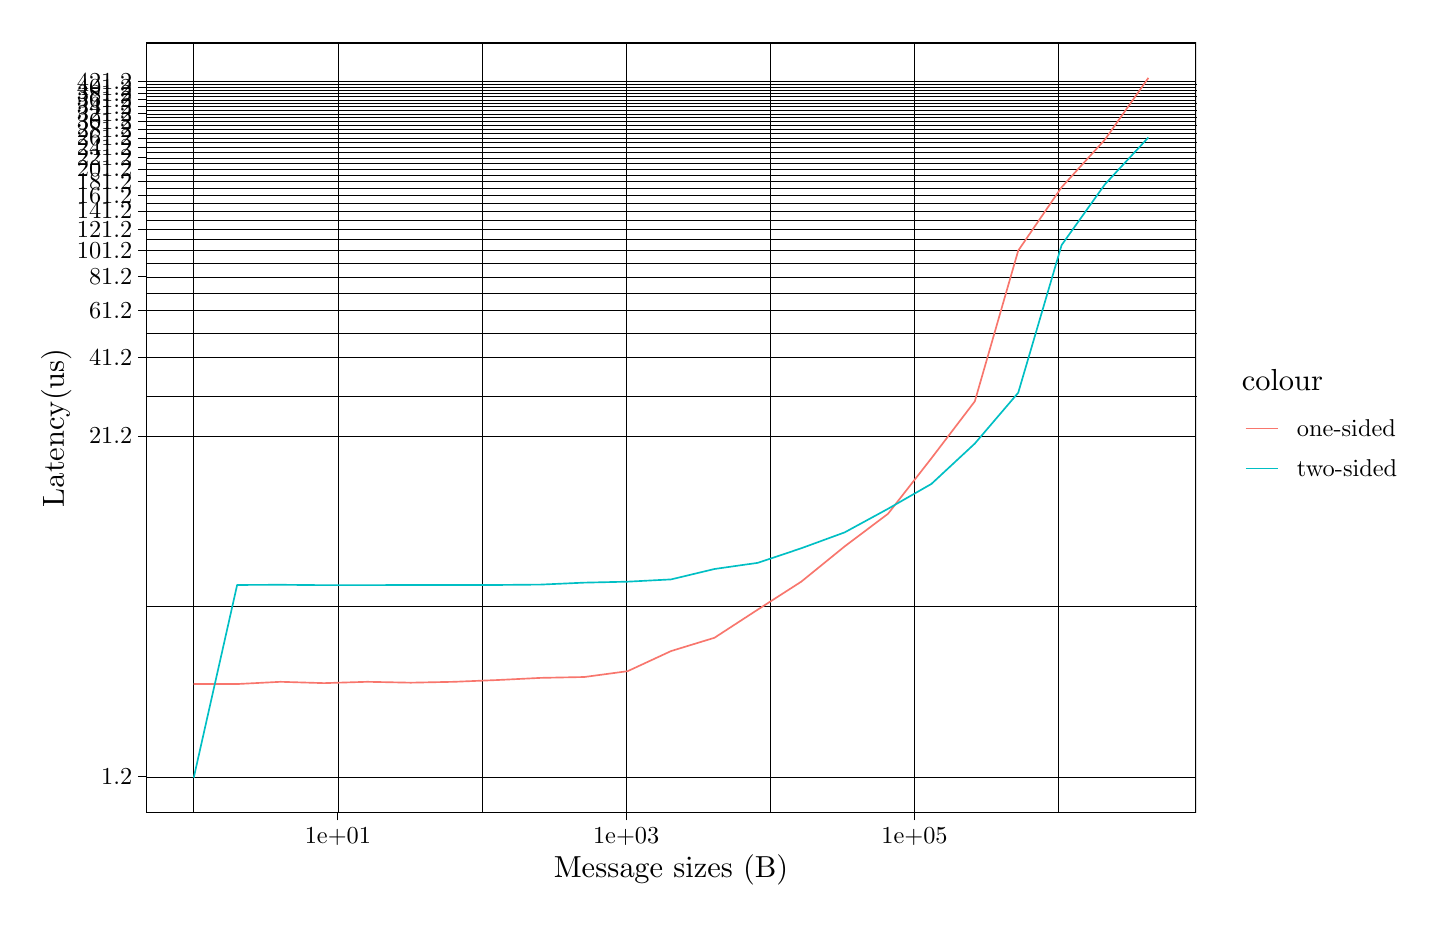
\begin{tikzpicture}[x=1pt,y=1pt]
\definecolor{fillColor}{RGB}{255,255,255}
\path[use as bounding box,fill=fillColor,fill opacity=0.00] (0,0) rectangle (505.89,314.37);
\begin{scope}
\path[clip] (  0.00,  0.00) rectangle (505.89,314.37);
\definecolor{drawColor}{RGB}{255,255,255}
\definecolor{fillColor}{RGB}{255,255,255}

\path[draw=drawColor,line width= 0.6pt,line join=round,line cap=round,fill=fillColor] (  0.00,  0.00) rectangle (505.89,314.37);
\end{scope}
\begin{scope}
\path[clip] ( 42.76, 30.72) rectangle (422.22,308.87);
\definecolor{fillColor}{RGB}{255,255,255}

\path[fill=fillColor] ( 42.76, 30.72) rectangle (422.22,308.87);
\definecolor{drawColor}{RGB}{0,0,0}

\path[draw=drawColor,line width= 0.0pt,line join=round] ( 42.76,105.27) --
	(422.22,105.27);

\path[draw=drawColor,line width= 0.0pt,line join=round] ( 42.76,181.04) --
	(422.22,181.04);

\path[draw=drawColor,line width= 0.0pt,line join=round] ( 42.76,203.76) --
	(422.22,203.76);

\path[draw=drawColor,line width= 0.0pt,line join=round] ( 42.76,218.30) --
	(422.22,218.30);

\path[draw=drawColor,line width= 0.0pt,line join=round] ( 42.76,229.08) --
	(422.22,229.08);

\path[draw=drawColor,line width= 0.0pt,line join=round] ( 42.76,237.66) --
	(422.22,237.66);

\path[draw=drawColor,line width= 0.0pt,line join=round] ( 42.76,244.80) --
	(422.22,244.80);

\path[draw=drawColor,line width= 0.0pt,line join=round] ( 42.76,250.91) --
	(422.22,250.91);

\path[draw=drawColor,line width= 0.0pt,line join=round] ( 42.76,256.26) --
	(422.22,256.26);

\path[draw=drawColor,line width= 0.0pt,line join=round] ( 42.76,261.01) --
	(422.22,261.01);

\path[draw=drawColor,line width= 0.0pt,line join=round] ( 42.76,265.28) --
	(422.22,265.28);

\path[draw=drawColor,line width= 0.0pt,line join=round] ( 42.76,269.17) --
	(422.22,269.17);

\path[draw=drawColor,line width= 0.0pt,line join=round] ( 42.76,272.73) --
	(422.22,272.73);

\path[draw=drawColor,line width= 0.0pt,line join=round] ( 42.76,276.02) --
	(422.22,276.02);

\path[draw=drawColor,line width= 0.0pt,line join=round] ( 42.76,279.07) --
	(422.22,279.07);

\path[draw=drawColor,line width= 0.0pt,line join=round] ( 42.76,281.92) --
	(422.22,281.92);

\path[draw=drawColor,line width= 0.0pt,line join=round] ( 42.76,284.60) --
	(422.22,284.60);

\path[draw=drawColor,line width= 0.0pt,line join=round] ( 42.76,287.11) --
	(422.22,287.11);

\path[draw=drawColor,line width= 0.0pt,line join=round] ( 42.76,289.49) --
	(422.22,289.49);

\path[draw=drawColor,line width= 0.0pt,line join=round] ( 42.76,291.74) --
	(422.22,291.74);

\path[draw=drawColor,line width= 0.0pt,line join=round] ( 42.76,293.88) --
	(422.22,293.88);

\path[draw=drawColor,line width= 0.0pt,line join=round] ( 60.01, 30.72) --
	( 60.01,308.87);

\path[draw=drawColor,line width= 0.0pt,line join=round] (164.18, 30.72) --
	(164.18,308.87);

\path[draw=drawColor,line width= 0.0pt,line join=round] (268.36, 30.72) --
	(268.36,308.87);

\path[draw=drawColor,line width= 0.0pt,line join=round] (372.54, 30.72) --
	(372.54,308.87);

\path[draw=drawColor,line width= 0.1pt,line join=round] ( 42.76, 43.73) --
	(422.22, 43.73);

\path[draw=drawColor,line width= 0.1pt,line join=round] ( 42.76,166.81) --
	(422.22,166.81);

\path[draw=drawColor,line width= 0.1pt,line join=round] ( 42.76,195.28) --
	(422.22,195.28);

\path[draw=drawColor,line width= 0.1pt,line join=round] ( 42.76,212.24) --
	(422.22,212.24);

\path[draw=drawColor,line width= 0.1pt,line join=round] ( 42.76,224.36) --
	(422.22,224.36);

\path[draw=drawColor,line width= 0.1pt,line join=round] ( 42.76,233.80) --
	(422.22,233.80);

\path[draw=drawColor,line width= 0.1pt,line join=round] ( 42.76,241.53) --
	(422.22,241.53);

\path[draw=drawColor,line width= 0.1pt,line join=round] ( 42.76,248.08) --
	(422.22,248.08);

\path[draw=drawColor,line width= 0.1pt,line join=round] ( 42.76,253.75) --
	(422.22,253.75);

\path[draw=drawColor,line width= 0.1pt,line join=round] ( 42.76,258.77) --
	(422.22,258.77);

\path[draw=drawColor,line width= 0.1pt,line join=round] ( 42.76,263.25) --
	(422.22,263.25);

\path[draw=drawColor,line width= 0.1pt,line join=round] ( 42.76,267.31) --
	(422.22,267.31);

\path[draw=drawColor,line width= 0.1pt,line join=round] ( 42.76,271.02) --
	(422.22,271.02);

\path[draw=drawColor,line width= 0.1pt,line join=round] ( 42.76,274.44) --
	(422.22,274.44);

\path[draw=drawColor,line width= 0.1pt,line join=round] ( 42.76,277.60) --
	(422.22,277.60);

\path[draw=drawColor,line width= 0.1pt,line join=round] ( 42.76,280.55) --
	(422.22,280.55);

\path[draw=drawColor,line width= 0.1pt,line join=round] ( 42.76,283.30) --
	(422.22,283.30);

\path[draw=drawColor,line width= 0.1pt,line join=round] ( 42.76,285.89) --
	(422.22,285.89);

\path[draw=drawColor,line width= 0.1pt,line join=round] ( 42.76,288.33) --
	(422.22,288.33);

\path[draw=drawColor,line width= 0.1pt,line join=round] ( 42.76,290.64) --
	(422.22,290.64);

\path[draw=drawColor,line width= 0.1pt,line join=round] ( 42.76,292.83) --
	(422.22,292.83);

\path[draw=drawColor,line width= 0.1pt,line join=round] ( 42.76,294.92) --
	(422.22,294.92);

\path[draw=drawColor,line width= 0.1pt,line join=round] (112.10, 30.72) --
	(112.10,308.87);

\path[draw=drawColor,line width= 0.1pt,line join=round] (216.27, 30.72) --
	(216.27,308.87);

\path[draw=drawColor,line width= 0.1pt,line join=round] (320.45, 30.72) --
	(320.45,308.87);
\definecolor{drawColor}{RGB}{248,118,109}

\path[draw=drawColor,line width= 0.6pt,line join=round] ( 60.01, 77.19) --
	( 75.69, 77.19) --
	( 91.37, 78.00) --
	(107.05, 77.52) --
	(122.73, 78.00) --
	(138.41, 77.68) --
	(154.09, 78.00) --
	(169.77, 78.64) --
	(185.45, 79.42) --
	(201.13, 79.73) --
	(216.81, 81.84) --
	(232.49, 89.11) --
	(248.17, 93.91) --
	(263.85,104.11) --
	(279.53,114.18) --
	(295.21,126.92) --
	(310.89,138.72) --
	(326.57,158.78) --
	(342.25,179.35) --
	(357.93,233.81) --
	(373.61,256.71) --
	(389.29,273.96) --
	(404.97,296.23);
\definecolor{drawColor}{RGB}{0,191,196}

\path[draw=drawColor,line width= 0.6pt,line join=round] ( 60.01, 43.37) --
	( 75.69,112.99) --
	( 91.37,113.06) --
	(107.05,112.92) --
	(122.73,112.92) --
	(138.41,112.99) --
	(154.09,112.99) --
	(169.77,112.99) --
	(185.45,113.13) --
	(201.13,113.83) --
	(216.81,114.18) --
	(232.49,115.00) --
	(248.17,118.76) --
	(263.85,120.99) --
	(279.53,126.25) --
	(295.21,131.99) --
	(310.89,140.52) --
	(326.57,149.51) --
	(342.25,164.09) --
	(357.93,182.45) --
	(373.61,235.81) --
	(389.29,257.80) --
	(404.97,274.70);
\definecolor{drawColor}{RGB}{0,0,0}

\path[draw=drawColor,line width= 0.6pt,line join=round,line cap=round] ( 42.76, 30.72) rectangle (422.22,308.87);
\end{scope}
\begin{scope}
\path[clip] (  0.00,  0.00) rectangle (505.89,314.37);
\definecolor{drawColor}{RGB}{0,0,0}

\node[text=drawColor,anchor=base west,inner sep=0pt, outer sep=0pt, scale=  0.88] at ( 26.57, 40.90) {1.2};

\node[text=drawColor,anchor=base west,inner sep=0pt, outer sep=0pt, scale=  0.88] at ( 22.17,163.98) {21.2};

\node[text=drawColor,anchor=base west,inner sep=0pt, outer sep=0pt, scale=  0.88] at ( 22.17,192.46) {41.2};

\node[text=drawColor,anchor=base west,inner sep=0pt, outer sep=0pt, scale=  0.88] at ( 22.17,209.42) {61.2};

\node[text=drawColor,anchor=base west,inner sep=0pt, outer sep=0pt, scale=  0.88] at ( 22.17,221.54) {81.2};

\node[text=drawColor,anchor=base west,inner sep=0pt, outer sep=0pt, scale=  0.88] at ( 17.77,230.98) {101.2};

\node[text=drawColor,anchor=base west,inner sep=0pt, outer sep=0pt, scale=  0.88] at ( 17.77,238.71) {121.2};

\node[text=drawColor,anchor=base west,inner sep=0pt, outer sep=0pt, scale=  0.88] at ( 17.77,245.25) {141.2};

\node[text=drawColor,anchor=base west,inner sep=0pt, outer sep=0pt, scale=  0.88] at ( 17.77,250.93) {161.2};

\node[text=drawColor,anchor=base west,inner sep=0pt, outer sep=0pt, scale=  0.88] at ( 17.77,255.94) {181.2};

\node[text=drawColor,anchor=base west,inner sep=0pt, outer sep=0pt, scale=  0.88] at ( 17.77,260.43) {201.2};

\node[text=drawColor,anchor=base west,inner sep=0pt, outer sep=0pt, scale=  0.88] at ( 17.77,264.49) {221.2};

\node[text=drawColor,anchor=base west,inner sep=0pt, outer sep=0pt, scale=  0.88] at ( 17.77,268.20) {241.2};

\node[text=drawColor,anchor=base west,inner sep=0pt, outer sep=0pt, scale=  0.88] at ( 17.77,271.62) {261.2};

\node[text=drawColor,anchor=base west,inner sep=0pt, outer sep=0pt, scale=  0.88] at ( 17.77,274.78) {281.2};

\node[text=drawColor,anchor=base west,inner sep=0pt, outer sep=0pt, scale=  0.88] at ( 17.77,277.72) {301.2};

\node[text=drawColor,anchor=base west,inner sep=0pt, outer sep=0pt, scale=  0.88] at ( 17.77,280.48) {321.2};

\node[text=drawColor,anchor=base west,inner sep=0pt, outer sep=0pt, scale=  0.88] at ( 17.77,283.07) {341.2};

\node[text=drawColor,anchor=base west,inner sep=0pt, outer sep=0pt, scale=  0.88] at ( 17.77,285.51) {361.2};

\node[text=drawColor,anchor=base west,inner sep=0pt, outer sep=0pt, scale=  0.88] at ( 17.77,287.82) {381.2};

\node[text=drawColor,anchor=base west,inner sep=0pt, outer sep=0pt, scale=  0.88] at ( 17.77,290.01) {401.2};

\node[text=drawColor,anchor=base west,inner sep=0pt, outer sep=0pt, scale=  0.88] at ( 17.77,292.09) {421.2};
\end{scope}
\begin{scope}
\path[clip] (  0.00,  0.00) rectangle (505.89,314.37);
\definecolor{drawColor}{RGB}{0,0,0}

\path[draw=drawColor,line width= 0.3pt,line join=round] ( 40.01, 43.73) --
	( 42.76, 43.73);

\path[draw=drawColor,line width= 0.3pt,line join=round] ( 40.01,166.81) --
	( 42.76,166.81);

\path[draw=drawColor,line width= 0.3pt,line join=round] ( 40.01,195.28) --
	( 42.76,195.28);

\path[draw=drawColor,line width= 0.3pt,line join=round] ( 40.01,212.24) --
	( 42.76,212.24);

\path[draw=drawColor,line width= 0.3pt,line join=round] ( 40.01,224.36) --
	( 42.76,224.36);

\path[draw=drawColor,line width= 0.3pt,line join=round] ( 40.01,233.80) --
	( 42.76,233.80);

\path[draw=drawColor,line width= 0.3pt,line join=round] ( 40.01,241.53) --
	( 42.76,241.53);

\path[draw=drawColor,line width= 0.3pt,line join=round] ( 40.01,248.08) --
	( 42.76,248.08);

\path[draw=drawColor,line width= 0.3pt,line join=round] ( 40.01,253.75) --
	( 42.76,253.75);

\path[draw=drawColor,line width= 0.3pt,line join=round] ( 40.01,258.77) --
	( 42.76,258.77);

\path[draw=drawColor,line width= 0.3pt,line join=round] ( 40.01,263.25) --
	( 42.76,263.25);

\path[draw=drawColor,line width= 0.3pt,line join=round] ( 40.01,267.31) --
	( 42.76,267.31);

\path[draw=drawColor,line width= 0.3pt,line join=round] ( 40.01,271.02) --
	( 42.76,271.02);

\path[draw=drawColor,line width= 0.3pt,line join=round] ( 40.01,274.44) --
	( 42.76,274.44);

\path[draw=drawColor,line width= 0.3pt,line join=round] ( 40.01,277.60) --
	( 42.76,277.60);

\path[draw=drawColor,line width= 0.3pt,line join=round] ( 40.01,280.55) --
	( 42.76,280.55);

\path[draw=drawColor,line width= 0.3pt,line join=round] ( 40.01,283.30) --
	( 42.76,283.30);

\path[draw=drawColor,line width= 0.3pt,line join=round] ( 40.01,285.89) --
	( 42.76,285.89);

\path[draw=drawColor,line width= 0.3pt,line join=round] ( 40.01,288.33) --
	( 42.76,288.33);

\path[draw=drawColor,line width= 0.3pt,line join=round] ( 40.01,290.64) --
	( 42.76,290.64);

\path[draw=drawColor,line width= 0.3pt,line join=round] ( 40.01,292.83) --
	( 42.76,292.83);

\path[draw=drawColor,line width= 0.3pt,line join=round] ( 40.01,294.92) --
	( 42.76,294.92);
\end{scope}
\begin{scope}
\path[clip] (  0.00,  0.00) rectangle (505.89,314.37);
\definecolor{drawColor}{RGB}{0,0,0}

\path[draw=drawColor,line width= 0.3pt,line join=round] (112.10, 27.97) --
	(112.10, 30.72);

\path[draw=drawColor,line width= 0.3pt,line join=round] (216.27, 27.97) --
	(216.27, 30.72);

\path[draw=drawColor,line width= 0.3pt,line join=round] (320.45, 27.97) --
	(320.45, 30.72);
\end{scope}
\begin{scope}
\path[clip] (  0.00,  0.00) rectangle (505.89,314.37);
\definecolor{drawColor}{RGB}{0,0,0}

\node[text=drawColor,anchor=base,inner sep=0pt, outer sep=0pt, scale=  0.88] at (112.10, 19.71) {1e+01};

\node[text=drawColor,anchor=base,inner sep=0pt, outer sep=0pt, scale=  0.88] at (216.27, 19.71) {1e+03};

\node[text=drawColor,anchor=base,inner sep=0pt, outer sep=0pt, scale=  0.88] at (320.45, 19.71) {1e+05};
\end{scope}
\begin{scope}
\path[clip] (  0.00,  0.00) rectangle (505.89,314.37);
\definecolor{drawColor}{RGB}{0,0,0}

\node[text=drawColor,anchor=base,inner sep=0pt, outer sep=0pt, scale=  1.10] at (232.49,  7.44) {Message sizes (B)};
\end{scope}
\begin{scope}
\path[clip] (  0.00,  0.00) rectangle (505.89,314.37);
\definecolor{drawColor}{RGB}{0,0,0}

\node[text=drawColor,rotate= 90.00,anchor=base,inner sep=0pt, outer sep=0pt, scale=  1.10] at ( 13.08,169.80) {Latency(us)};
\end{scope}
\begin{scope}
\path[clip] (  0.00,  0.00) rectangle (505.89,314.37);
\definecolor{fillColor}{RGB}{255,255,255}

\path[fill=fillColor] (433.22,142.34) rectangle (500.39,197.26);
\end{scope}
\begin{scope}
\path[clip] (  0.00,  0.00) rectangle (505.89,314.37);
\definecolor{drawColor}{RGB}{0,0,0}

\node[text=drawColor,anchor=base west,inner sep=0pt, outer sep=0pt, scale=  1.10] at (438.72,183.22) {colour};
\end{scope}
\begin{scope}
\path[clip] (  0.00,  0.00) rectangle (505.89,314.37);
\definecolor{fillColor}{RGB}{255,255,255}

\path[fill=fillColor] (438.72,162.29) rectangle (453.17,176.74);
\end{scope}
\begin{scope}
\path[clip] (  0.00,  0.00) rectangle (505.89,314.37);
\definecolor{drawColor}{RGB}{248,118,109}

\path[draw=drawColor,line width= 0.6pt,line join=round] (440.16,169.52) -- (451.73,169.52);
\end{scope}
\begin{scope}
\path[clip] (  0.00,  0.00) rectangle (505.89,314.37);
\definecolor{drawColor}{RGB}{248,118,109}

\path[draw=drawColor,line width= 0.6pt,line join=round] (440.16,169.52) -- (451.73,169.52);
\end{scope}
\begin{scope}
\path[clip] (  0.00,  0.00) rectangle (505.89,314.37);
\definecolor{fillColor}{RGB}{255,255,255}

\path[fill=fillColor] (438.72,147.84) rectangle (453.17,162.29);
\end{scope}
\begin{scope}
\path[clip] (  0.00,  0.00) rectangle (505.89,314.37);
\definecolor{drawColor}{RGB}{0,191,196}

\path[draw=drawColor,line width= 0.6pt,line join=round] (440.16,155.06) -- (451.73,155.06);
\end{scope}
\begin{scope}
\path[clip] (  0.00,  0.00) rectangle (505.89,314.37);
\definecolor{drawColor}{RGB}{0,191,196}

\path[draw=drawColor,line width= 0.6pt,line join=round] (440.16,155.06) -- (451.73,155.06);
\end{scope}
\begin{scope}
\path[clip] (  0.00,  0.00) rectangle (505.89,314.37);
\definecolor{drawColor}{RGB}{0,0,0}

\node[text=drawColor,anchor=base west,inner sep=0pt, outer sep=0pt, scale=  0.88] at (458.67,166.49) {one-sided};
\end{scope}
\begin{scope}
\path[clip] (  0.00,  0.00) rectangle (505.89,314.37);
\definecolor{drawColor}{RGB}{0,0,0}

\node[text=drawColor,anchor=base west,inner sep=0pt, outer sep=0pt, scale=  0.88] at (458.67,152.03) {two-sided};
\end{scope}
\end{tikzpicture}

	\caption{2 node, latency, gpu-gpu, flush-local, create window, one-sided, two-sided comparisons}
\end{figure}

\begin{figure}
	% Created by tikzDevice version 0.10.1 on 2020-02-15 16:13:19
% !TEX encoding = UTF-8 Unicode
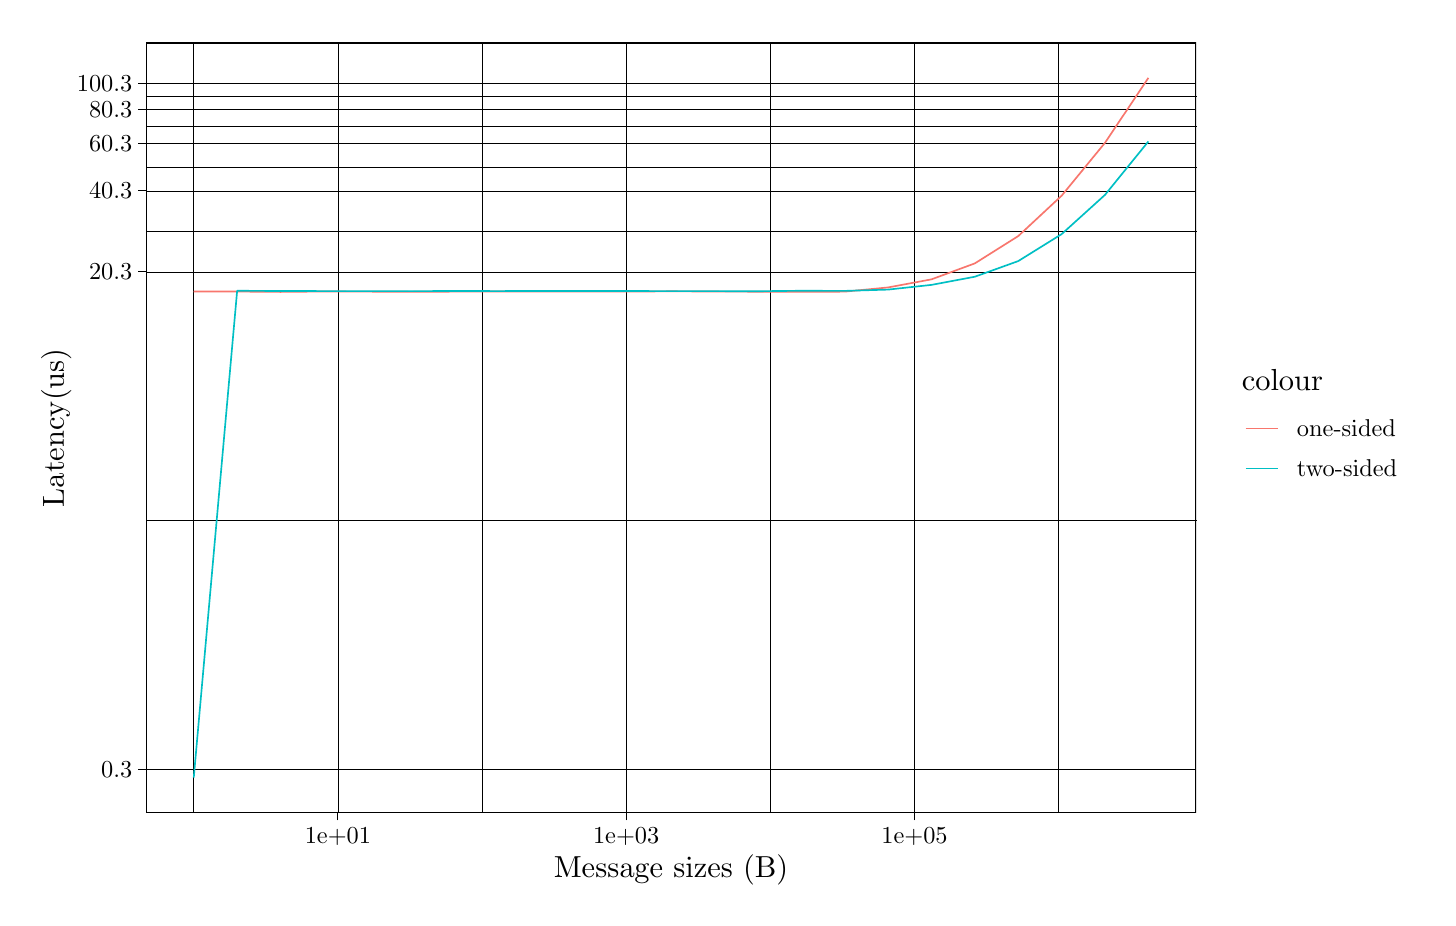
\begin{tikzpicture}[x=1pt,y=1pt]
\definecolor{fillColor}{RGB}{255,255,255}
\path[use as bounding box,fill=fillColor,fill opacity=0.00] (0,0) rectangle (505.89,314.37);
\begin{scope}
\path[clip] (  0.00,  0.00) rectangle (505.89,314.37);
\definecolor{drawColor}{RGB}{255,255,255}
\definecolor{fillColor}{RGB}{255,255,255}

\path[draw=drawColor,line width= 0.6pt,line join=round,line cap=round,fill=fillColor] (  0.00,  0.00) rectangle (505.89,314.37);
\end{scope}
\begin{scope}
\path[clip] ( 42.76, 30.72) rectangle (422.22,308.87);
\definecolor{fillColor}{RGB}{255,255,255}

\path[fill=fillColor] ( 42.76, 30.72) rectangle (422.22,308.87);
\definecolor{drawColor}{RGB}{0,0,0}

\path[draw=drawColor,line width= 0.0pt,line join=round] ( 42.76,136.22) --
	(422.22,136.22);

\path[draw=drawColor,line width= 0.0pt,line join=round] ( 42.76,240.75) --
	(422.22,240.75);

\path[draw=drawColor,line width= 0.0pt,line join=round] ( 42.76,263.98) --
	(422.22,263.98);

\path[draw=drawColor,line width= 0.0pt,line join=round] ( 42.76,278.69) --
	(422.22,278.69);

\path[draw=drawColor,line width= 0.0pt,line join=round] ( 42.76,289.54) --
	(422.22,289.54);

\path[draw=drawColor,line width= 0.0pt,line join=round] ( 60.01, 30.72) --
	( 60.01,308.87);

\path[draw=drawColor,line width= 0.0pt,line join=round] (164.18, 30.72) --
	(164.18,308.87);

\path[draw=drawColor,line width= 0.0pt,line join=round] (268.36, 30.72) --
	(268.36,308.87);

\path[draw=drawColor,line width= 0.0pt,line join=round] (372.54, 30.72) --
	(372.54,308.87);

\path[draw=drawColor,line width= 0.1pt,line join=round] ( 42.76, 46.31) --
	(422.22, 46.31);

\path[draw=drawColor,line width= 0.1pt,line join=round] ( 42.76,226.13) --
	(422.22,226.13);

\path[draw=drawColor,line width= 0.1pt,line join=round] ( 42.76,255.38) --
	(422.22,255.38);

\path[draw=drawColor,line width= 0.1pt,line join=round] ( 42.76,272.58) --
	(422.22,272.58);

\path[draw=drawColor,line width= 0.1pt,line join=round] ( 42.76,284.80) --
	(422.22,284.80);

\path[draw=drawColor,line width= 0.1pt,line join=round] ( 42.76,294.29) --
	(422.22,294.29);

\path[draw=drawColor,line width= 0.1pt,line join=round] (112.10, 30.72) --
	(112.10,308.87);

\path[draw=drawColor,line width= 0.1pt,line join=round] (216.27, 30.72) --
	(216.27,308.87);

\path[draw=drawColor,line width= 0.1pt,line join=round] (320.45, 30.72) --
	(320.45,308.87);
\definecolor{drawColor}{RGB}{248,118,109}

\path[draw=drawColor,line width= 0.6pt,line join=round] ( 60.01,219.06) --
	( 75.69,219.01) --
	( 91.37,218.88) --
	(107.05,219.03) --
	(122.73,218.98) --
	(138.41,218.91) --
	(154.09,218.98) --
	(169.77,219.01) --
	(185.45,219.03) --
	(201.13,219.06) --
	(216.81,218.98) --
	(232.49,219.11) --
	(248.17,219.01) --
	(263.85,218.96) --
	(279.53,218.91) --
	(295.21,218.98) --
	(310.89,220.50) --
	(326.57,223.42) --
	(342.25,229.19) --
	(357.93,239.05) --
	(373.61,253.64) --
	(389.29,272.77) --
	(404.97,296.23);
\definecolor{drawColor}{RGB}{0,191,196}

\path[draw=drawColor,line width= 0.6pt,line join=round] ( 60.01, 43.37) --
	( 75.69,219.30) --
	( 91.37,219.21) --
	(107.05,219.18) --
	(122.73,219.16) --
	(138.41,219.16) --
	(154.09,219.21) --
	(169.77,219.18) --
	(185.45,219.21) --
	(201.13,219.21) --
	(216.81,219.21) --
	(232.49,219.16) --
	(248.17,219.16) --
	(263.85,219.13) --
	(279.53,219.30) --
	(295.21,219.25) --
	(310.89,219.72) --
	(326.57,221.42) --
	(342.25,224.37) --
	(357.93,230.02) --
	(373.61,239.76) --
	(389.29,253.95) --
	(404.97,273.26);
\definecolor{drawColor}{RGB}{0,0,0}

\path[draw=drawColor,line width= 0.6pt,line join=round,line cap=round] ( 42.76, 30.72) rectangle (422.22,308.87);
\end{scope}
\begin{scope}
\path[clip] (  0.00,  0.00) rectangle (505.89,314.37);
\definecolor{drawColor}{RGB}{0,0,0}

\node[text=drawColor,anchor=base west,inner sep=0pt, outer sep=0pt, scale=  0.88] at ( 26.57, 43.49) {0.3};

\node[text=drawColor,anchor=base west,inner sep=0pt, outer sep=0pt, scale=  0.88] at ( 22.17,223.30) {20.3};

\node[text=drawColor,anchor=base west,inner sep=0pt, outer sep=0pt, scale=  0.88] at ( 22.17,252.56) {40.3};

\node[text=drawColor,anchor=base west,inner sep=0pt, outer sep=0pt, scale=  0.88] at ( 22.17,269.75) {60.3};

\node[text=drawColor,anchor=base west,inner sep=0pt, outer sep=0pt, scale=  0.88] at ( 22.17,281.97) {80.3};

\node[text=drawColor,anchor=base west,inner sep=0pt, outer sep=0pt, scale=  0.88] at ( 17.77,291.46) {100.3};
\end{scope}
\begin{scope}
\path[clip] (  0.00,  0.00) rectangle (505.89,314.37);
\definecolor{drawColor}{RGB}{0,0,0}

\path[draw=drawColor,line width= 0.3pt,line join=round] ( 40.01, 46.31) --
	( 42.76, 46.31);

\path[draw=drawColor,line width= 0.3pt,line join=round] ( 40.01,226.13) --
	( 42.76,226.13);

\path[draw=drawColor,line width= 0.3pt,line join=round] ( 40.01,255.38) --
	( 42.76,255.38);

\path[draw=drawColor,line width= 0.3pt,line join=round] ( 40.01,272.58) --
	( 42.76,272.58);

\path[draw=drawColor,line width= 0.3pt,line join=round] ( 40.01,284.80) --
	( 42.76,284.80);

\path[draw=drawColor,line width= 0.3pt,line join=round] ( 40.01,294.29) --
	( 42.76,294.29);
\end{scope}
\begin{scope}
\path[clip] (  0.00,  0.00) rectangle (505.89,314.37);
\definecolor{drawColor}{RGB}{0,0,0}

\path[draw=drawColor,line width= 0.3pt,line join=round] (112.10, 27.97) --
	(112.10, 30.72);

\path[draw=drawColor,line width= 0.3pt,line join=round] (216.27, 27.97) --
	(216.27, 30.72);

\path[draw=drawColor,line width= 0.3pt,line join=round] (320.45, 27.97) --
	(320.45, 30.72);
\end{scope}
\begin{scope}
\path[clip] (  0.00,  0.00) rectangle (505.89,314.37);
\definecolor{drawColor}{RGB}{0,0,0}

\node[text=drawColor,anchor=base,inner sep=0pt, outer sep=0pt, scale=  0.88] at (112.10, 19.71) {1e+01};

\node[text=drawColor,anchor=base,inner sep=0pt, outer sep=0pt, scale=  0.88] at (216.27, 19.71) {1e+03};

\node[text=drawColor,anchor=base,inner sep=0pt, outer sep=0pt, scale=  0.88] at (320.45, 19.71) {1e+05};
\end{scope}
\begin{scope}
\path[clip] (  0.00,  0.00) rectangle (505.89,314.37);
\definecolor{drawColor}{RGB}{0,0,0}

\node[text=drawColor,anchor=base,inner sep=0pt, outer sep=0pt, scale=  1.10] at (232.49,  7.44) {Message sizes (B)};
\end{scope}
\begin{scope}
\path[clip] (  0.00,  0.00) rectangle (505.89,314.37);
\definecolor{drawColor}{RGB}{0,0,0}

\node[text=drawColor,rotate= 90.00,anchor=base,inner sep=0pt, outer sep=0pt, scale=  1.10] at ( 13.08,169.80) {Latency(us)};
\end{scope}
\begin{scope}
\path[clip] (  0.00,  0.00) rectangle (505.89,314.37);
\definecolor{fillColor}{RGB}{255,255,255}

\path[fill=fillColor] (433.22,142.34) rectangle (500.39,197.26);
\end{scope}
\begin{scope}
\path[clip] (  0.00,  0.00) rectangle (505.89,314.37);
\definecolor{drawColor}{RGB}{0,0,0}

\node[text=drawColor,anchor=base west,inner sep=0pt, outer sep=0pt, scale=  1.10] at (438.72,183.22) {colour};
\end{scope}
\begin{scope}
\path[clip] (  0.00,  0.00) rectangle (505.89,314.37);
\definecolor{fillColor}{RGB}{255,255,255}

\path[fill=fillColor] (438.72,162.29) rectangle (453.17,176.74);
\end{scope}
\begin{scope}
\path[clip] (  0.00,  0.00) rectangle (505.89,314.37);
\definecolor{drawColor}{RGB}{248,118,109}

\path[draw=drawColor,line width= 0.6pt,line join=round] (440.16,169.52) -- (451.73,169.52);
\end{scope}
\begin{scope}
\path[clip] (  0.00,  0.00) rectangle (505.89,314.37);
\definecolor{drawColor}{RGB}{248,118,109}

\path[draw=drawColor,line width= 0.6pt,line join=round] (440.16,169.52) -- (451.73,169.52);
\end{scope}
\begin{scope}
\path[clip] (  0.00,  0.00) rectangle (505.89,314.37);
\definecolor{fillColor}{RGB}{255,255,255}

\path[fill=fillColor] (438.72,147.84) rectangle (453.17,162.29);
\end{scope}
\begin{scope}
\path[clip] (  0.00,  0.00) rectangle (505.89,314.37);
\definecolor{drawColor}{RGB}{0,191,196}

\path[draw=drawColor,line width= 0.6pt,line join=round] (440.16,155.06) -- (451.73,155.06);
\end{scope}
\begin{scope}
\path[clip] (  0.00,  0.00) rectangle (505.89,314.37);
\definecolor{drawColor}{RGB}{0,191,196}

\path[draw=drawColor,line width= 0.6pt,line join=round] (440.16,155.06) -- (451.73,155.06);
\end{scope}
\begin{scope}
\path[clip] (  0.00,  0.00) rectangle (505.89,314.37);
\definecolor{drawColor}{RGB}{0,0,0}

\node[text=drawColor,anchor=base west,inner sep=0pt, outer sep=0pt, scale=  0.88] at (458.67,166.49) {one-sided};
\end{scope}
\begin{scope}
\path[clip] (  0.00,  0.00) rectangle (505.89,314.37);
\definecolor{drawColor}{RGB}{0,0,0}

\node[text=drawColor,anchor=base west,inner sep=0pt, outer sep=0pt, scale=  0.88] at (458.67,152.03) {two-sided};
\end{scope}
\end{tikzpicture}

	\caption{1 node, latency, gpu-gpu, flush-local, create window, one-sided, two-sided comparisons}
\end{figure}

\begin{figure}
	% Created by tikzDevice version 0.10.1 on 2020-02-15 16:17:05
% !TEX encoding = UTF-8 Unicode
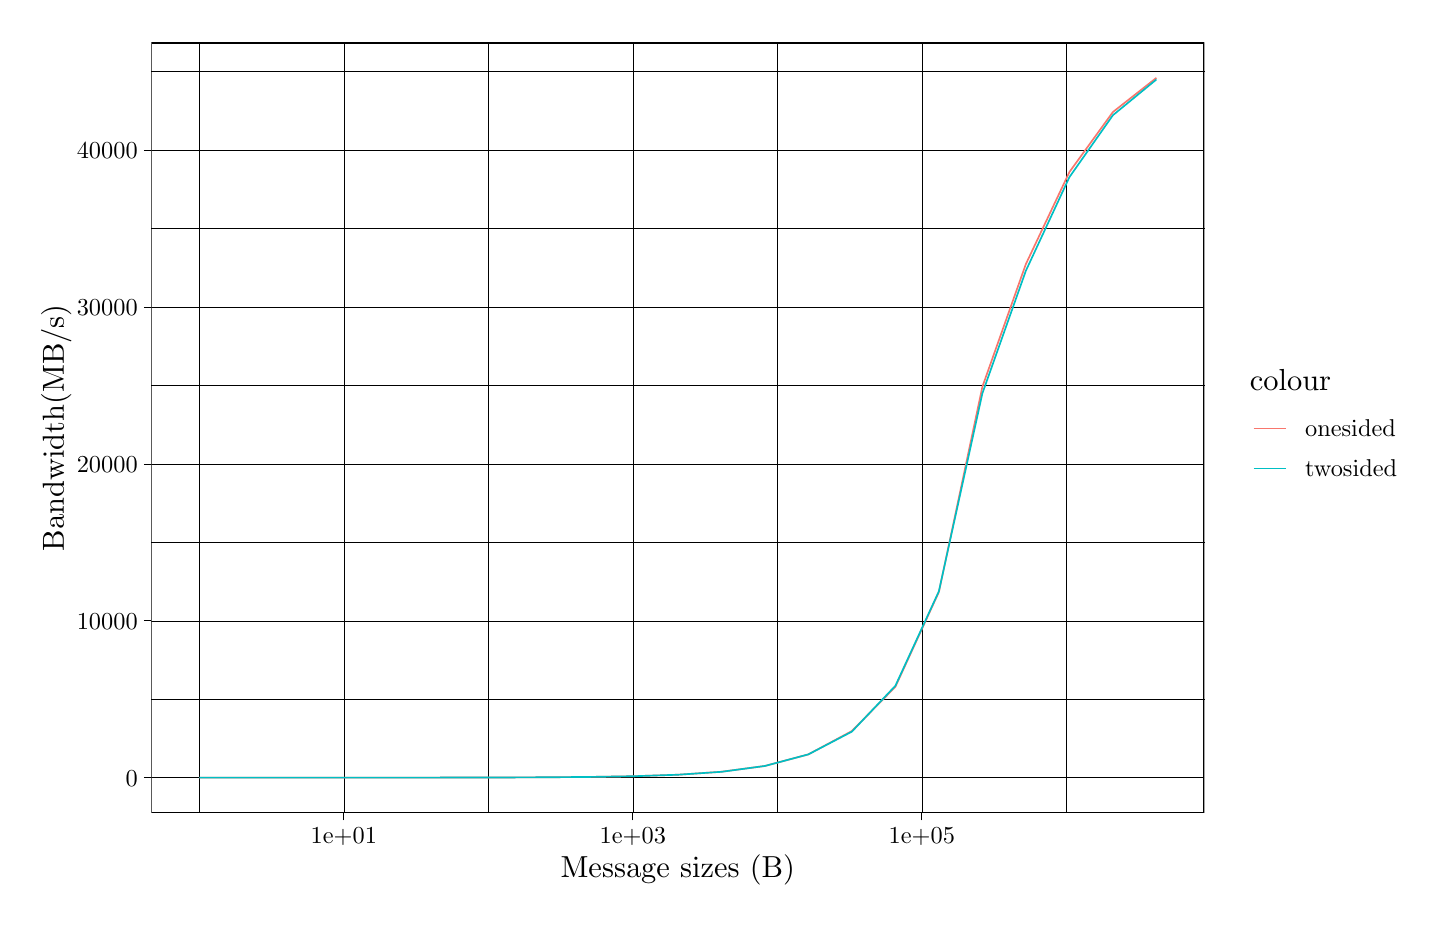
\begin{tikzpicture}[x=1pt,y=1pt]
\definecolor{fillColor}{RGB}{255,255,255}
\path[use as bounding box,fill=fillColor,fill opacity=0.00] (0,0) rectangle (505.89,314.37);
\begin{scope}
\path[clip] (  0.00,  0.00) rectangle (505.89,314.37);
\definecolor{drawColor}{RGB}{255,255,255}
\definecolor{fillColor}{RGB}{255,255,255}

\path[draw=drawColor,line width= 0.6pt,line join=round,line cap=round,fill=fillColor] (  0.00,  0.00) rectangle (505.89,314.37);
\end{scope}
\begin{scope}
\path[clip] ( 44.71, 30.72) rectangle (425.15,308.87);
\definecolor{fillColor}{RGB}{255,255,255}

\path[fill=fillColor] ( 44.71, 30.72) rectangle (425.15,308.87);
\definecolor{drawColor}{RGB}{0,0,0}

\path[draw=drawColor,line width= 0.0pt,line join=round] ( 44.71, 71.70) --
	(425.15, 71.70);

\path[draw=drawColor,line width= 0.0pt,line join=round] ( 44.71,128.36) --
	(425.15,128.36);

\path[draw=drawColor,line width= 0.0pt,line join=round] ( 44.71,185.03) --
	(425.15,185.03);

\path[draw=drawColor,line width= 0.0pt,line join=round] ( 44.71,241.69) --
	(425.15,241.69);

\path[draw=drawColor,line width= 0.0pt,line join=round] ( 44.71,298.36) --
	(425.15,298.36);

\path[draw=drawColor,line width= 0.0pt,line join=round] ( 62.01, 30.72) --
	( 62.01,308.87);

\path[draw=drawColor,line width= 0.0pt,line join=round] (166.45, 30.72) --
	(166.45,308.87);

\path[draw=drawColor,line width= 0.0pt,line join=round] (270.90, 30.72) --
	(270.90,308.87);

\path[draw=drawColor,line width= 0.0pt,line join=round] (375.34, 30.72) --
	(375.34,308.87);

\path[draw=drawColor,line width= 0.1pt,line join=round] ( 44.71, 43.37) --
	(425.15, 43.37);

\path[draw=drawColor,line width= 0.1pt,line join=round] ( 44.71,100.03) --
	(425.15,100.03);

\path[draw=drawColor,line width= 0.1pt,line join=round] ( 44.71,156.70) --
	(425.15,156.70);

\path[draw=drawColor,line width= 0.1pt,line join=round] ( 44.71,213.36) --
	(425.15,213.36);

\path[draw=drawColor,line width= 0.1pt,line join=round] ( 44.71,270.02) --
	(425.15,270.02);

\path[draw=drawColor,line width= 0.1pt,line join=round] (114.23, 30.72) --
	(114.23,308.87);

\path[draw=drawColor,line width= 0.1pt,line join=round] (218.67, 30.72) --
	(218.67,308.87);

\path[draw=drawColor,line width= 0.1pt,line join=round] (323.12, 30.72) --
	(323.12,308.87);
\definecolor{drawColor}{RGB}{248,118,109}

\path[draw=drawColor,line width= 0.6pt,line join=round] ( 62.01, 43.37) --
	( 77.73, 43.37) --
	( 93.45, 43.37) --
	(109.17, 43.37) --
	(124.89, 43.38) --
	(140.61, 43.38) --
	(156.33, 43.40) --
	(172.05, 43.43) --
	(187.77, 43.50) --
	(203.49, 43.63) --
	(219.21, 43.89) --
	(234.93, 44.42) --
	(250.65, 45.49) --
	(266.37, 47.59) --
	(282.09, 51.77) --
	(297.81, 60.20) --
	(313.54, 76.19) --
	(329.26,110.43) --
	(344.98,184.61) --
	(360.70,228.96) --
	(376.42,262.19) --
	(392.14,283.88) --
	(407.86,296.23);
\definecolor{drawColor}{RGB}{0,191,196}

\path[draw=drawColor,line width= 0.6pt,line join=round] ( 62.01, 43.37) --
	( 77.73, 43.37) --
	( 93.45, 43.37) --
	(109.17, 43.37) --
	(124.89, 43.38) --
	(140.61, 43.38) --
	(156.33, 43.40) --
	(172.05, 43.43) --
	(187.77, 43.50) --
	(203.49, 43.63) --
	(219.21, 43.89) --
	(234.93, 44.42) --
	(250.65, 45.47) --
	(266.37, 47.58) --
	(282.09, 51.77) --
	(297.81, 59.98) --
	(313.54, 76.56) --
	(329.26,110.70) --
	(344.98,182.22) --
	(360.70,226.54) --
	(376.42,260.34) --
	(392.14,282.73) --
	(407.86,295.64);
\definecolor{drawColor}{RGB}{0,0,0}

\path[draw=drawColor,line width= 0.6pt,line join=round,line cap=round] ( 44.71, 30.72) rectangle (425.15,308.87);
\end{scope}
\begin{scope}
\path[clip] (  0.00,  0.00) rectangle (505.89,314.37);
\definecolor{drawColor}{RGB}{0,0,0}

\node[text=drawColor,anchor=base east,inner sep=0pt, outer sep=0pt, scale=  0.88] at ( 39.76, 40.34) {0};

\node[text=drawColor,anchor=base east,inner sep=0pt, outer sep=0pt, scale=  0.88] at ( 39.76, 97.00) {10000};

\node[text=drawColor,anchor=base east,inner sep=0pt, outer sep=0pt, scale=  0.88] at ( 39.76,153.67) {20000};

\node[text=drawColor,anchor=base east,inner sep=0pt, outer sep=0pt, scale=  0.88] at ( 39.76,210.33) {30000};

\node[text=drawColor,anchor=base east,inner sep=0pt, outer sep=0pt, scale=  0.88] at ( 39.76,266.99) {40000};
\end{scope}
\begin{scope}
\path[clip] (  0.00,  0.00) rectangle (505.89,314.37);
\definecolor{drawColor}{RGB}{0,0,0}

\path[draw=drawColor,line width= 0.3pt,line join=round] ( 41.96, 43.37) --
	( 44.71, 43.37);

\path[draw=drawColor,line width= 0.3pt,line join=round] ( 41.96,100.03) --
	( 44.71,100.03);

\path[draw=drawColor,line width= 0.3pt,line join=round] ( 41.96,156.70) --
	( 44.71,156.70);

\path[draw=drawColor,line width= 0.3pt,line join=round] ( 41.96,213.36) --
	( 44.71,213.36);

\path[draw=drawColor,line width= 0.3pt,line join=round] ( 41.96,270.02) --
	( 44.71,270.02);
\end{scope}
\begin{scope}
\path[clip] (  0.00,  0.00) rectangle (505.89,314.37);
\definecolor{drawColor}{RGB}{0,0,0}

\path[draw=drawColor,line width= 0.3pt,line join=round] (114.23, 27.97) --
	(114.23, 30.72);

\path[draw=drawColor,line width= 0.3pt,line join=round] (218.67, 27.97) --
	(218.67, 30.72);

\path[draw=drawColor,line width= 0.3pt,line join=round] (323.12, 27.97) --
	(323.12, 30.72);
\end{scope}
\begin{scope}
\path[clip] (  0.00,  0.00) rectangle (505.89,314.37);
\definecolor{drawColor}{RGB}{0,0,0}

\node[text=drawColor,anchor=base,inner sep=0pt, outer sep=0pt, scale=  0.88] at (114.23, 19.71) {1e+01};

\node[text=drawColor,anchor=base,inner sep=0pt, outer sep=0pt, scale=  0.88] at (218.67, 19.71) {1e+03};

\node[text=drawColor,anchor=base,inner sep=0pt, outer sep=0pt, scale=  0.88] at (323.12, 19.71) {1e+05};
\end{scope}
\begin{scope}
\path[clip] (  0.00,  0.00) rectangle (505.89,314.37);
\definecolor{drawColor}{RGB}{0,0,0}

\node[text=drawColor,anchor=base,inner sep=0pt, outer sep=0pt, scale=  1.10] at (234.93,  7.44) {Message sizes (B)};
\end{scope}
\begin{scope}
\path[clip] (  0.00,  0.00) rectangle (505.89,314.37);
\definecolor{drawColor}{RGB}{0,0,0}

\node[text=drawColor,rotate= 90.00,anchor=base,inner sep=0pt, outer sep=0pt, scale=  1.10] at ( 13.08,169.80) {Bandwidth(MB/s)};
\end{scope}
\begin{scope}
\path[clip] (  0.00,  0.00) rectangle (505.89,314.37);
\definecolor{fillColor}{RGB}{255,255,255}

\path[fill=fillColor] (436.15,142.34) rectangle (500.39,197.26);
\end{scope}
\begin{scope}
\path[clip] (  0.00,  0.00) rectangle (505.89,314.37);
\definecolor{drawColor}{RGB}{0,0,0}

\node[text=drawColor,anchor=base west,inner sep=0pt, outer sep=0pt, scale=  1.10] at (441.65,183.22) {colour};
\end{scope}
\begin{scope}
\path[clip] (  0.00,  0.00) rectangle (505.89,314.37);
\definecolor{fillColor}{RGB}{255,255,255}

\path[fill=fillColor] (441.65,162.29) rectangle (456.10,176.74);
\end{scope}
\begin{scope}
\path[clip] (  0.00,  0.00) rectangle (505.89,314.37);
\definecolor{drawColor}{RGB}{248,118,109}

\path[draw=drawColor,line width= 0.6pt,line join=round] (443.10,169.52) -- (454.66,169.52);
\end{scope}
\begin{scope}
\path[clip] (  0.00,  0.00) rectangle (505.89,314.37);
\definecolor{drawColor}{RGB}{248,118,109}

\path[draw=drawColor,line width= 0.6pt,line join=round] (443.10,169.52) -- (454.66,169.52);
\end{scope}
\begin{scope}
\path[clip] (  0.00,  0.00) rectangle (505.89,314.37);
\definecolor{fillColor}{RGB}{255,255,255}

\path[fill=fillColor] (441.65,147.84) rectangle (456.10,162.29);
\end{scope}
\begin{scope}
\path[clip] (  0.00,  0.00) rectangle (505.89,314.37);
\definecolor{drawColor}{RGB}{0,191,196}

\path[draw=drawColor,line width= 0.6pt,line join=round] (443.10,155.06) -- (454.66,155.06);
\end{scope}
\begin{scope}
\path[clip] (  0.00,  0.00) rectangle (505.89,314.37);
\definecolor{drawColor}{RGB}{0,191,196}

\path[draw=drawColor,line width= 0.6pt,line join=round] (443.10,155.06) -- (454.66,155.06);
\end{scope}
\begin{scope}
\path[clip] (  0.00,  0.00) rectangle (505.89,314.37);
\definecolor{drawColor}{RGB}{0,0,0}

\node[text=drawColor,anchor=base west,inner sep=0pt, outer sep=0pt, scale=  0.88] at (461.60,166.49) {onesided};
\end{scope}
\begin{scope}
\path[clip] (  0.00,  0.00) rectangle (505.89,314.37);
\definecolor{drawColor}{RGB}{0,0,0}

\node[text=drawColor,anchor=base west,inner sep=0pt, outer sep=0pt, scale=  0.88] at (461.60,152.03) {twosided};
\end{scope}
\end{tikzpicture}

	\caption{1 node, bw, gpu-gpu, flush-local, create window, one-sided, two-sided comparisons}
\end{figure}

\begin{figure}
	% Created by tikzDevice version 0.10.1 on 2020-02-15 16:19:10
% !TEX encoding = UTF-8 Unicode
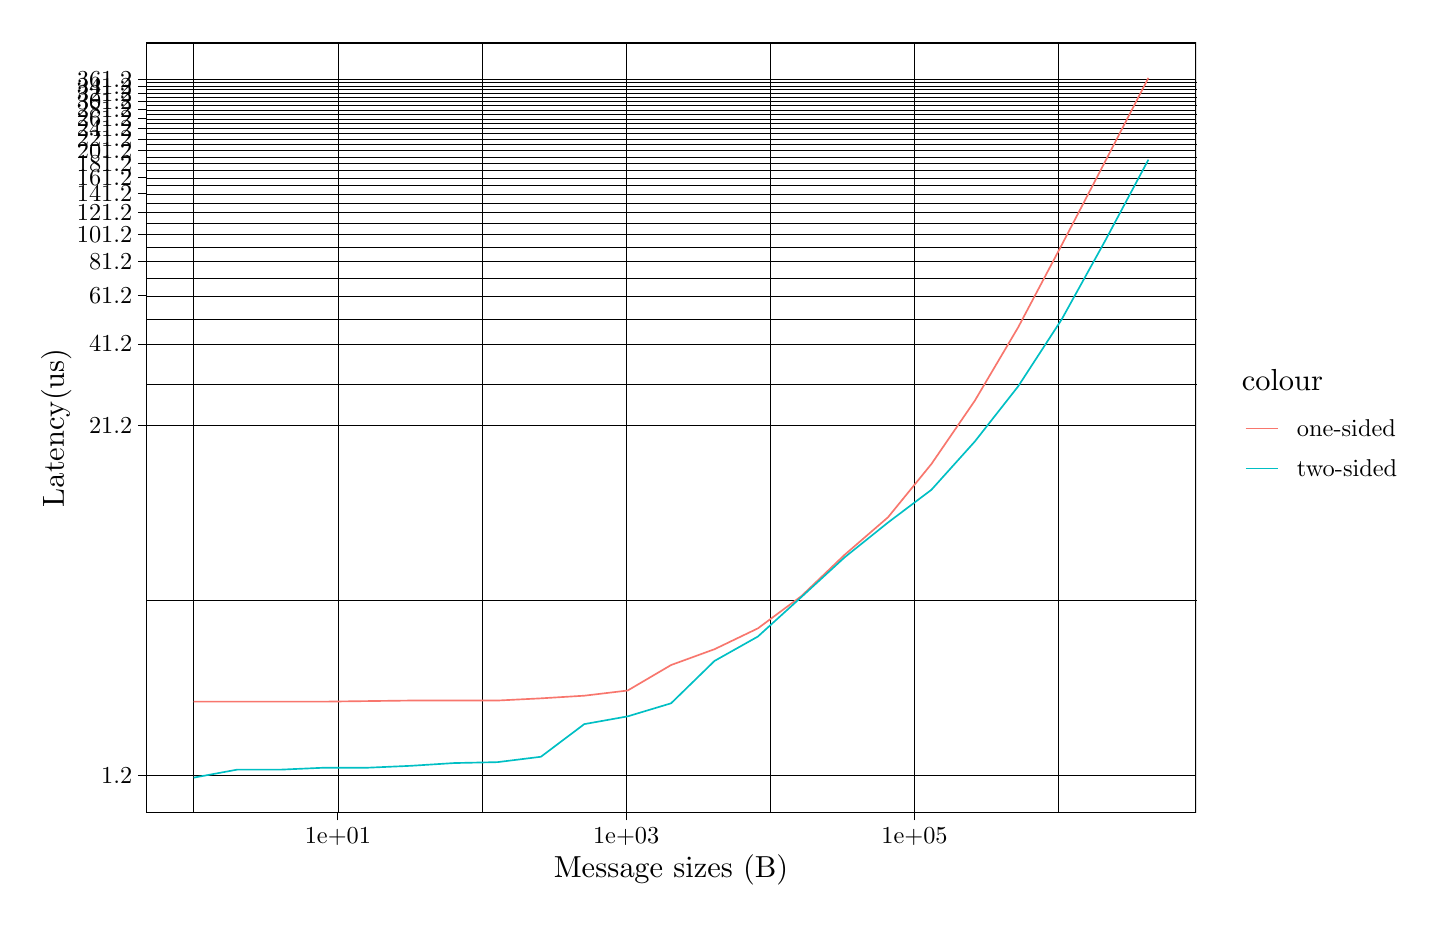
\begin{tikzpicture}[x=1pt,y=1pt]
\definecolor{fillColor}{RGB}{255,255,255}
\path[use as bounding box,fill=fillColor,fill opacity=0.00] (0,0) rectangle (505.89,314.37);
\begin{scope}
\path[clip] (  0.00,  0.00) rectangle (505.89,314.37);
\definecolor{drawColor}{RGB}{255,255,255}
\definecolor{fillColor}{RGB}{255,255,255}

\path[draw=drawColor,line width= 0.6pt,line join=round,line cap=round,fill=fillColor] (  0.00,  0.00) rectangle (505.89,314.37);
\end{scope}
\begin{scope}
\path[clip] ( 42.76, 30.72) rectangle (422.22,308.87);
\definecolor{fillColor}{RGB}{255,255,255}

\path[fill=fillColor] ( 42.76, 30.72) rectangle (422.22,308.87);
\definecolor{drawColor}{RGB}{0,0,0}

\path[draw=drawColor,line width= 0.0pt,line join=round] ( 42.76,107.41) --
	(422.22,107.41);

\path[draw=drawColor,line width= 0.0pt,line join=round] ( 42.76,185.37) --
	(422.22,185.37);

\path[draw=drawColor,line width= 0.0pt,line join=round] ( 42.76,208.74) --
	(422.22,208.74);

\path[draw=drawColor,line width= 0.0pt,line join=round] ( 42.76,223.70) --
	(422.22,223.70);

\path[draw=drawColor,line width= 0.0pt,line join=round] ( 42.76,234.78) --
	(422.22,234.78);

\path[draw=drawColor,line width= 0.0pt,line join=round] ( 42.76,243.61) --
	(422.22,243.61);

\path[draw=drawColor,line width= 0.0pt,line join=round] ( 42.76,250.96) --
	(422.22,250.96);

\path[draw=drawColor,line width= 0.0pt,line join=round] ( 42.76,257.24) --
	(422.22,257.24);

\path[draw=drawColor,line width= 0.0pt,line join=round] ( 42.76,262.74) --
	(422.22,262.74);

\path[draw=drawColor,line width= 0.0pt,line join=round] ( 42.76,267.63) --
	(422.22,267.63);

\path[draw=drawColor,line width= 0.0pt,line join=round] ( 42.76,272.03) --
	(422.22,272.03);

\path[draw=drawColor,line width= 0.0pt,line join=round] ( 42.76,276.02) --
	(422.22,276.02);

\path[draw=drawColor,line width= 0.0pt,line join=round] ( 42.76,279.69) --
	(422.22,279.69);

\path[draw=drawColor,line width= 0.0pt,line join=round] ( 42.76,283.07) --
	(422.22,283.07);

\path[draw=drawColor,line width= 0.0pt,line join=round] ( 42.76,286.21) --
	(422.22,286.21);

\path[draw=drawColor,line width= 0.0pt,line join=round] ( 42.76,289.14) --
	(422.22,289.14);

\path[draw=drawColor,line width= 0.0pt,line join=round] ( 42.76,291.89) --
	(422.22,291.89);

\path[draw=drawColor,line width= 0.0pt,line join=round] ( 42.76,294.48) --
	(422.22,294.48);

\path[draw=drawColor,line width= 0.0pt,line join=round] ( 60.01, 30.72) --
	( 60.01,308.87);

\path[draw=drawColor,line width= 0.0pt,line join=round] (164.18, 30.72) --
	(164.18,308.87);

\path[draw=drawColor,line width= 0.0pt,line join=round] (268.36, 30.72) --
	(268.36,308.87);

\path[draw=drawColor,line width= 0.0pt,line join=round] (372.54, 30.72) --
	(372.54,308.87);

\path[draw=drawColor,line width= 0.1pt,line join=round] ( 42.76, 44.11) --
	(422.22, 44.11);

\path[draw=drawColor,line width= 0.1pt,line join=round] ( 42.76,170.72) --
	(422.22,170.72);

\path[draw=drawColor,line width= 0.1pt,line join=round] ( 42.76,200.02) --
	(422.22,200.02);

\path[draw=drawColor,line width= 0.1pt,line join=round] ( 42.76,217.46) --
	(422.22,217.46);

\path[draw=drawColor,line width= 0.1pt,line join=round] ( 42.76,229.93) --
	(422.22,229.93);

\path[draw=drawColor,line width= 0.1pt,line join=round] ( 42.76,239.64) --
	(422.22,239.64);

\path[draw=drawColor,line width= 0.1pt,line join=round] ( 42.76,247.59) --
	(422.22,247.59);

\path[draw=drawColor,line width= 0.1pt,line join=round] ( 42.76,254.32) --
	(422.22,254.32);

\path[draw=drawColor,line width= 0.1pt,line join=round] ( 42.76,260.16) --
	(422.22,260.16);

\path[draw=drawColor,line width= 0.1pt,line join=round] ( 42.76,265.32) --
	(422.22,265.32);

\path[draw=drawColor,line width= 0.1pt,line join=round] ( 42.76,269.94) --
	(422.22,269.94);

\path[draw=drawColor,line width= 0.1pt,line join=round] ( 42.76,274.11) --
	(422.22,274.11);

\path[draw=drawColor,line width= 0.1pt,line join=round] ( 42.76,277.93) --
	(422.22,277.93);

\path[draw=drawColor,line width= 0.1pt,line join=round] ( 42.76,281.44) --
	(422.22,281.44);

\path[draw=drawColor,line width= 0.1pt,line join=round] ( 42.76,284.70) --
	(422.22,284.70);

\path[draw=drawColor,line width= 0.1pt,line join=round] ( 42.76,287.73) --
	(422.22,287.73);

\path[draw=drawColor,line width= 0.1pt,line join=round] ( 42.76,290.56) --
	(422.22,290.56);

\path[draw=drawColor,line width= 0.1pt,line join=round] ( 42.76,293.22) --
	(422.22,293.22);

\path[draw=drawColor,line width= 0.1pt,line join=round] ( 42.76,295.73) --
	(422.22,295.73);

\path[draw=drawColor,line width= 0.1pt,line join=round] (112.10, 30.72) --
	(112.10,308.87);

\path[draw=drawColor,line width= 0.1pt,line join=round] (216.27, 30.72) --
	(216.27,308.87);

\path[draw=drawColor,line width= 0.1pt,line join=round] (320.45, 30.72) --
	(320.45,308.87);
\definecolor{drawColor}{RGB}{248,118,109}

\path[draw=drawColor,line width= 0.6pt,line join=round] ( 60.01, 70.83) --
	( 75.69, 70.83) --
	( 91.37, 70.83) --
	(107.05, 70.83) --
	(122.73, 71.03) --
	(138.41, 71.23) --
	(154.09, 71.23) --
	(169.77, 71.23) --
	(185.45, 72.02) --
	(201.13, 72.98) --
	(216.81, 74.85) --
	(232.49, 84.06) --
	(248.17, 89.77) --
	(263.85, 97.30) --
	(279.53,108.93) --
	(295.21,123.90) --
	(310.89,137.46) --
	(326.57,156.71) --
	(342.25,179.58) --
	(357.93,206.12) --
	(373.61,235.78) --
	(389.29,265.90) --
	(404.97,296.23);
\definecolor{drawColor}{RGB}{0,191,196}

\path[draw=drawColor,line width= 0.6pt,line join=round] ( 60.01, 43.37) --
	( 75.69, 46.26) --
	( 91.37, 46.26) --
	(107.05, 46.95) --
	(122.73, 46.95) --
	(138.41, 47.64) --
	(154.09, 48.64) --
	(169.77, 48.97) --
	(185.45, 50.91) --
	(201.13, 62.71) --
	(216.81, 65.51) --
	(232.49, 70.23) --
	(248.17, 85.53) --
	(263.85, 94.35) --
	(279.53,108.59) --
	(295.21,122.98) --
	(310.89,135.56) --
	(326.57,147.39) --
	(342.25,164.83) --
	(357.93,184.79) --
	(373.61,208.91) --
	(389.29,237.27) --
	(404.97,266.66);
\definecolor{drawColor}{RGB}{0,0,0}

\path[draw=drawColor,line width= 0.6pt,line join=round,line cap=round] ( 42.76, 30.72) rectangle (422.22,308.87);
\end{scope}
\begin{scope}
\path[clip] (  0.00,  0.00) rectangle (505.89,314.37);
\definecolor{drawColor}{RGB}{0,0,0}

\node[text=drawColor,anchor=base west,inner sep=0pt, outer sep=0pt, scale=  0.88] at ( 26.57, 41.29) {1.2};

\node[text=drawColor,anchor=base west,inner sep=0pt, outer sep=0pt, scale=  0.88] at ( 22.17,167.90) {21.2};

\node[text=drawColor,anchor=base west,inner sep=0pt, outer sep=0pt, scale=  0.88] at ( 22.17,197.19) {41.2};

\node[text=drawColor,anchor=base west,inner sep=0pt, outer sep=0pt, scale=  0.88] at ( 22.17,214.64) {61.2};

\node[text=drawColor,anchor=base west,inner sep=0pt, outer sep=0pt, scale=  0.88] at ( 22.17,227.11) {81.2};

\node[text=drawColor,anchor=base west,inner sep=0pt, outer sep=0pt, scale=  0.88] at ( 17.77,236.82) {101.2};

\node[text=drawColor,anchor=base west,inner sep=0pt, outer sep=0pt, scale=  0.88] at ( 17.77,244.77) {121.2};

\node[text=drawColor,anchor=base west,inner sep=0pt, outer sep=0pt, scale=  0.88] at ( 17.77,251.50) {141.2};

\node[text=drawColor,anchor=base west,inner sep=0pt, outer sep=0pt, scale=  0.88] at ( 17.77,257.34) {161.2};

\node[text=drawColor,anchor=base west,inner sep=0pt, outer sep=0pt, scale=  0.88] at ( 17.77,262.50) {181.2};

\node[text=drawColor,anchor=base west,inner sep=0pt, outer sep=0pt, scale=  0.88] at ( 17.77,267.11) {201.2};

\node[text=drawColor,anchor=base west,inner sep=0pt, outer sep=0pt, scale=  0.88] at ( 17.77,271.29) {221.2};

\node[text=drawColor,anchor=base west,inner sep=0pt, outer sep=0pt, scale=  0.88] at ( 17.77,275.11) {241.2};

\node[text=drawColor,anchor=base west,inner sep=0pt, outer sep=0pt, scale=  0.88] at ( 17.77,278.62) {261.2};

\node[text=drawColor,anchor=base west,inner sep=0pt, outer sep=0pt, scale=  0.88] at ( 17.77,281.87) {281.2};

\node[text=drawColor,anchor=base west,inner sep=0pt, outer sep=0pt, scale=  0.88] at ( 17.77,284.90) {301.2};

\node[text=drawColor,anchor=base west,inner sep=0pt, outer sep=0pt, scale=  0.88] at ( 17.77,287.74) {321.2};

\node[text=drawColor,anchor=base west,inner sep=0pt, outer sep=0pt, scale=  0.88] at ( 17.77,290.40) {341.2};

\node[text=drawColor,anchor=base west,inner sep=0pt, outer sep=0pt, scale=  0.88] at ( 17.77,292.91) {361.2};
\end{scope}
\begin{scope}
\path[clip] (  0.00,  0.00) rectangle (505.89,314.37);
\definecolor{drawColor}{RGB}{0,0,0}

\path[draw=drawColor,line width= 0.3pt,line join=round] ( 40.01, 44.11) --
	( 42.76, 44.11);

\path[draw=drawColor,line width= 0.3pt,line join=round] ( 40.01,170.72) --
	( 42.76,170.72);

\path[draw=drawColor,line width= 0.3pt,line join=round] ( 40.01,200.02) --
	( 42.76,200.02);

\path[draw=drawColor,line width= 0.3pt,line join=round] ( 40.01,217.46) --
	( 42.76,217.46);

\path[draw=drawColor,line width= 0.3pt,line join=round] ( 40.01,229.93) --
	( 42.76,229.93);

\path[draw=drawColor,line width= 0.3pt,line join=round] ( 40.01,239.64) --
	( 42.76,239.64);

\path[draw=drawColor,line width= 0.3pt,line join=round] ( 40.01,247.59) --
	( 42.76,247.59);

\path[draw=drawColor,line width= 0.3pt,line join=round] ( 40.01,254.32) --
	( 42.76,254.32);

\path[draw=drawColor,line width= 0.3pt,line join=round] ( 40.01,260.16) --
	( 42.76,260.16);

\path[draw=drawColor,line width= 0.3pt,line join=round] ( 40.01,265.32) --
	( 42.76,265.32);

\path[draw=drawColor,line width= 0.3pt,line join=round] ( 40.01,269.94) --
	( 42.76,269.94);

\path[draw=drawColor,line width= 0.3pt,line join=round] ( 40.01,274.11) --
	( 42.76,274.11);

\path[draw=drawColor,line width= 0.3pt,line join=round] ( 40.01,277.93) --
	( 42.76,277.93);

\path[draw=drawColor,line width= 0.3pt,line join=round] ( 40.01,281.44) --
	( 42.76,281.44);

\path[draw=drawColor,line width= 0.3pt,line join=round] ( 40.01,284.70) --
	( 42.76,284.70);

\path[draw=drawColor,line width= 0.3pt,line join=round] ( 40.01,287.73) --
	( 42.76,287.73);

\path[draw=drawColor,line width= 0.3pt,line join=round] ( 40.01,290.56) --
	( 42.76,290.56);

\path[draw=drawColor,line width= 0.3pt,line join=round] ( 40.01,293.22) --
	( 42.76,293.22);

\path[draw=drawColor,line width= 0.3pt,line join=round] ( 40.01,295.73) --
	( 42.76,295.73);
\end{scope}
\begin{scope}
\path[clip] (  0.00,  0.00) rectangle (505.89,314.37);
\definecolor{drawColor}{RGB}{0,0,0}

\path[draw=drawColor,line width= 0.3pt,line join=round] (112.10, 27.97) --
	(112.10, 30.72);

\path[draw=drawColor,line width= 0.3pt,line join=round] (216.27, 27.97) --
	(216.27, 30.72);

\path[draw=drawColor,line width= 0.3pt,line join=round] (320.45, 27.97) --
	(320.45, 30.72);
\end{scope}
\begin{scope}
\path[clip] (  0.00,  0.00) rectangle (505.89,314.37);
\definecolor{drawColor}{RGB}{0,0,0}

\node[text=drawColor,anchor=base,inner sep=0pt, outer sep=0pt, scale=  0.88] at (112.10, 19.71) {1e+01};

\node[text=drawColor,anchor=base,inner sep=0pt, outer sep=0pt, scale=  0.88] at (216.27, 19.71) {1e+03};

\node[text=drawColor,anchor=base,inner sep=0pt, outer sep=0pt, scale=  0.88] at (320.45, 19.71) {1e+05};
\end{scope}
\begin{scope}
\path[clip] (  0.00,  0.00) rectangle (505.89,314.37);
\definecolor{drawColor}{RGB}{0,0,0}

\node[text=drawColor,anchor=base,inner sep=0pt, outer sep=0pt, scale=  1.10] at (232.49,  7.44) {Message sizes (B)};
\end{scope}
\begin{scope}
\path[clip] (  0.00,  0.00) rectangle (505.89,314.37);
\definecolor{drawColor}{RGB}{0,0,0}

\node[text=drawColor,rotate= 90.00,anchor=base,inner sep=0pt, outer sep=0pt, scale=  1.10] at ( 13.08,169.80) {Latency(us)};
\end{scope}
\begin{scope}
\path[clip] (  0.00,  0.00) rectangle (505.89,314.37);
\definecolor{fillColor}{RGB}{255,255,255}

\path[fill=fillColor] (433.22,142.34) rectangle (500.39,197.26);
\end{scope}
\begin{scope}
\path[clip] (  0.00,  0.00) rectangle (505.89,314.37);
\definecolor{drawColor}{RGB}{0,0,0}

\node[text=drawColor,anchor=base west,inner sep=0pt, outer sep=0pt, scale=  1.10] at (438.72,183.22) {colour};
\end{scope}
\begin{scope}
\path[clip] (  0.00,  0.00) rectangle (505.89,314.37);
\definecolor{fillColor}{RGB}{255,255,255}

\path[fill=fillColor] (438.72,162.29) rectangle (453.17,176.74);
\end{scope}
\begin{scope}
\path[clip] (  0.00,  0.00) rectangle (505.89,314.37);
\definecolor{drawColor}{RGB}{248,118,109}

\path[draw=drawColor,line width= 0.6pt,line join=round] (440.16,169.52) -- (451.73,169.52);
\end{scope}
\begin{scope}
\path[clip] (  0.00,  0.00) rectangle (505.89,314.37);
\definecolor{drawColor}{RGB}{248,118,109}

\path[draw=drawColor,line width= 0.6pt,line join=round] (440.16,169.52) -- (451.73,169.52);
\end{scope}
\begin{scope}
\path[clip] (  0.00,  0.00) rectangle (505.89,314.37);
\definecolor{fillColor}{RGB}{255,255,255}

\path[fill=fillColor] (438.72,147.84) rectangle (453.17,162.29);
\end{scope}
\begin{scope}
\path[clip] (  0.00,  0.00) rectangle (505.89,314.37);
\definecolor{drawColor}{RGB}{0,191,196}

\path[draw=drawColor,line width= 0.6pt,line join=round] (440.16,155.06) -- (451.73,155.06);
\end{scope}
\begin{scope}
\path[clip] (  0.00,  0.00) rectangle (505.89,314.37);
\definecolor{drawColor}{RGB}{0,191,196}

\path[draw=drawColor,line width= 0.6pt,line join=round] (440.16,155.06) -- (451.73,155.06);
\end{scope}
\begin{scope}
\path[clip] (  0.00,  0.00) rectangle (505.89,314.37);
\definecolor{drawColor}{RGB}{0,0,0}

\node[text=drawColor,anchor=base west,inner sep=0pt, outer sep=0pt, scale=  0.88] at (458.67,166.49) {one-sided};
\end{scope}
\begin{scope}
\path[clip] (  0.00,  0.00) rectangle (505.89,314.37);
\definecolor{drawColor}{RGB}{0,0,0}

\node[text=drawColor,anchor=base west,inner sep=0pt, outer sep=0pt, scale=  0.88] at (458.67,152.03) {two-sided};
\end{scope}
\end{tikzpicture}

	\caption{2 node, latency, cpu-cpu, flush-local, create window, one-sided, two-sided comparisons}
\end{figure}

\begin{figure}
	% Created by tikzDevice version 0.10.1 on 2020-02-15 16:19:28
% !TEX encoding = UTF-8 Unicode
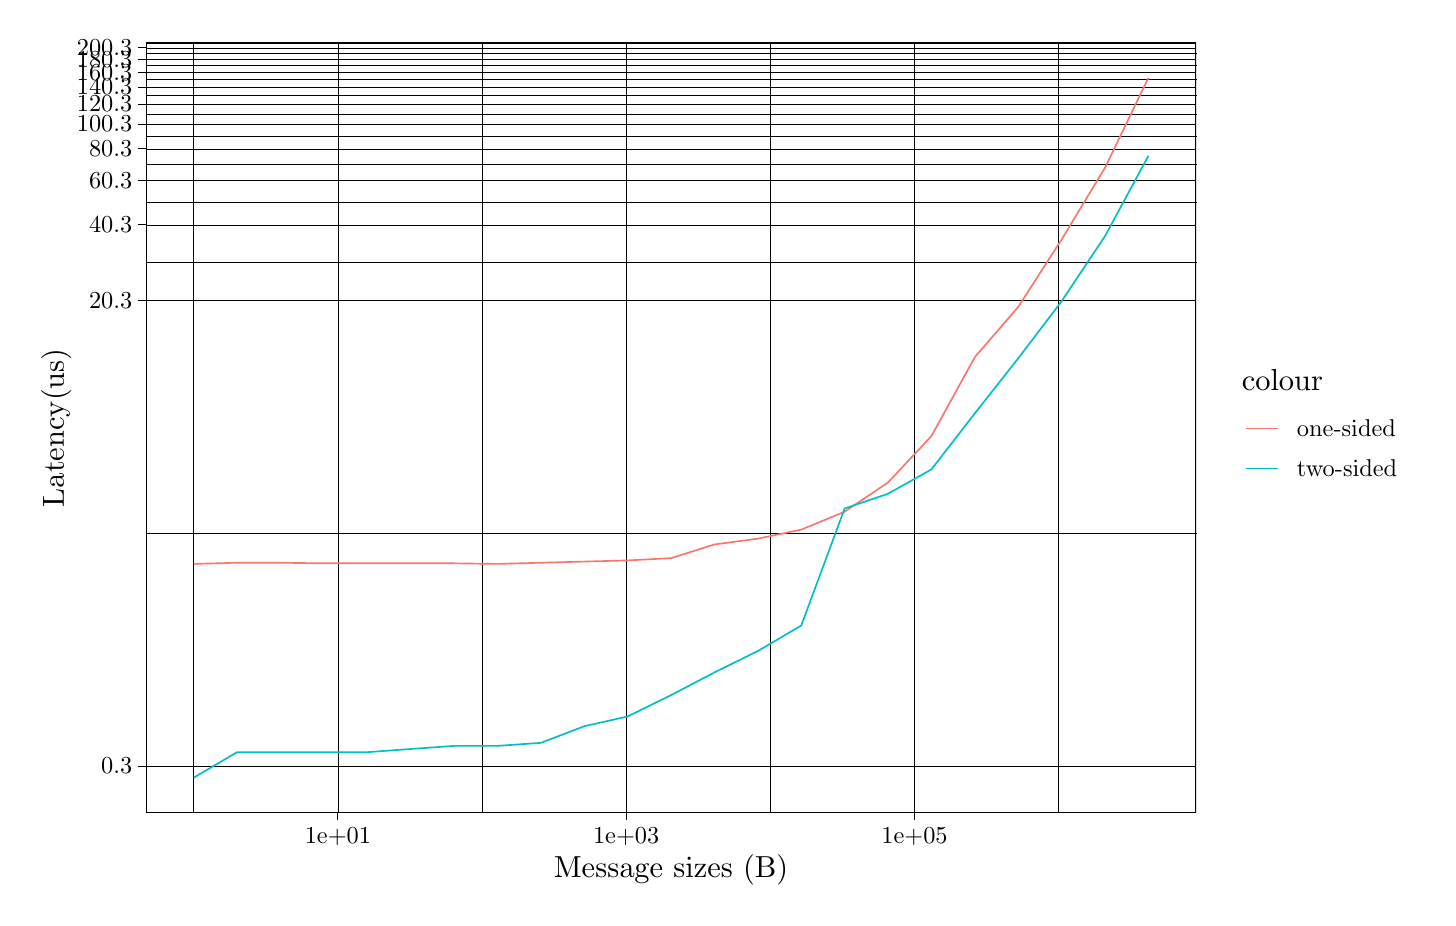
\begin{tikzpicture}[x=1pt,y=1pt]
\definecolor{fillColor}{RGB}{255,255,255}
\path[use as bounding box,fill=fillColor,fill opacity=0.00] (0,0) rectangle (505.89,314.37);
\begin{scope}
\path[clip] (  0.00,  0.00) rectangle (505.89,314.37);
\definecolor{drawColor}{RGB}{255,255,255}
\definecolor{fillColor}{RGB}{255,255,255}

\path[draw=drawColor,line width= 0.6pt,line join=round,line cap=round,fill=fillColor] (  0.00,  0.00) rectangle (505.89,314.37);
\end{scope}
\begin{scope}
\path[clip] ( 42.76, 30.72) rectangle (422.22,308.87);
\definecolor{fillColor}{RGB}{255,255,255}

\path[fill=fillColor] ( 42.76, 30.72) rectangle (422.22,308.87);
\definecolor{drawColor}{RGB}{0,0,0}

\path[draw=drawColor,line width= 0.0pt,line join=round] ( 42.76,131.67) --
	(422.22,131.67);

\path[draw=drawColor,line width= 0.0pt,line join=round] ( 42.76,229.45) --
	(422.22,229.45);

\path[draw=drawColor,line width= 0.0pt,line join=round] ( 42.76,251.17) --
	(422.22,251.17);

\path[draw=drawColor,line width= 0.0pt,line join=round] ( 42.76,264.93) --
	(422.22,264.93);

\path[draw=drawColor,line width= 0.0pt,line join=round] ( 42.76,275.08) --
	(422.22,275.08);

\path[draw=drawColor,line width= 0.0pt,line join=round] ( 42.76,283.15) --
	(422.22,283.15);

\path[draw=drawColor,line width= 0.0pt,line join=round] ( 42.76,289.84) --
	(422.22,289.84);

\path[draw=drawColor,line width= 0.0pt,line join=round] ( 42.76,295.57) --
	(422.22,295.57);

\path[draw=drawColor,line width= 0.0pt,line join=round] ( 42.76,300.58) --
	(422.22,300.58);

\path[draw=drawColor,line width= 0.0pt,line join=round] ( 42.76,305.02) --
	(422.22,305.02);

\path[draw=drawColor,line width= 0.0pt,line join=round] ( 60.01, 30.72) --
	( 60.01,308.87);

\path[draw=drawColor,line width= 0.0pt,line join=round] (164.18, 30.72) --
	(164.18,308.87);

\path[draw=drawColor,line width= 0.0pt,line join=round] (268.36, 30.72) --
	(268.36,308.87);

\path[draw=drawColor,line width= 0.0pt,line join=round] (372.54, 30.72) --
	(372.54,308.87);

\path[draw=drawColor,line width= 0.1pt,line join=round] ( 42.76, 47.57) --
	(422.22, 47.57);

\path[draw=drawColor,line width= 0.1pt,line join=round] ( 42.76,215.76) --
	(422.22,215.76);

\path[draw=drawColor,line width= 0.1pt,line join=round] ( 42.76,243.13) --
	(422.22,243.13);

\path[draw=drawColor,line width= 0.1pt,line join=round] ( 42.76,259.21) --
	(422.22,259.21);

\path[draw=drawColor,line width= 0.1pt,line join=round] ( 42.76,270.64) --
	(422.22,270.64);

\path[draw=drawColor,line width= 0.1pt,line join=round] ( 42.76,279.52) --
	(422.22,279.52);

\path[draw=drawColor,line width= 0.1pt,line join=round] ( 42.76,286.77) --
	(422.22,286.77);

\path[draw=drawColor,line width= 0.1pt,line join=round] ( 42.76,292.91) --
	(422.22,292.91);

\path[draw=drawColor,line width= 0.1pt,line join=round] ( 42.76,298.23) --
	(422.22,298.23);

\path[draw=drawColor,line width= 0.1pt,line join=round] ( 42.76,302.92) --
	(422.22,302.92);

\path[draw=drawColor,line width= 0.1pt,line join=round] ( 42.76,307.12) --
	(422.22,307.12);

\path[draw=drawColor,line width= 0.1pt,line join=round] (112.10, 30.72) --
	(112.10,308.87);

\path[draw=drawColor,line width= 0.1pt,line join=round] (216.27, 30.72) --
	(216.27,308.87);

\path[draw=drawColor,line width= 0.1pt,line join=round] (320.45, 30.72) --
	(320.45,308.87);
\definecolor{drawColor}{RGB}{248,118,109}

\path[draw=drawColor,line width= 0.6pt,line join=round] ( 60.01,120.60) --
	( 75.69,121.02) --
	( 91.37,121.02) --
	(107.05,120.81) --
	(122.73,120.81) --
	(138.41,120.81) --
	(154.09,120.81) --
	(169.77,120.60) --
	(185.45,121.02) --
	(201.13,121.44) --
	(216.81,121.86) --
	(232.49,122.68) --
	(248.17,127.63) --
	(263.85,129.72) --
	(279.53,132.98) --
	(295.21,139.46) --
	(310.89,150.03) --
	(326.57,166.79) --
	(342.25,195.31) --
	(357.93,213.46) --
	(373.61,237.82) --
	(389.29,263.76) --
	(404.97,296.23);
\definecolor{drawColor}{RGB}{0,191,196}

\path[draw=drawColor,line width= 0.6pt,line join=round] ( 60.01, 43.37) --
	( 75.69, 52.57) --
	( 91.37, 52.57) --
	(107.05, 52.57) --
	(122.73, 52.57) --
	(138.41, 53.72) --
	(154.09, 54.85) --
	(169.77, 54.85) --
	(185.45, 55.94) --
	(201.13, 61.94) --
	(216.81, 65.49) --
	(232.49, 73.19) --
	(248.17, 81.39) --
	(263.85, 89.13) --
	(279.53, 98.32) --
	(295.21,140.64) --
	(310.89,145.95) --
	(326.57,154.75) --
	(342.25,175.00) --
	(357.93,194.88) --
	(373.61,215.49) --
	(389.29,239.04) --
	(404.97,268.06);
\definecolor{drawColor}{RGB}{0,0,0}

\path[draw=drawColor,line width= 0.6pt,line join=round,line cap=round] ( 42.76, 30.72) rectangle (422.22,308.87);
\end{scope}
\begin{scope}
\path[clip] (  0.00,  0.00) rectangle (505.89,314.37);
\definecolor{drawColor}{RGB}{0,0,0}

\node[text=drawColor,anchor=base west,inner sep=0pt, outer sep=0pt, scale=  0.88] at ( 26.57, 44.75) {0.3};

\node[text=drawColor,anchor=base west,inner sep=0pt, outer sep=0pt, scale=  0.88] at ( 22.17,212.94) {20.3};

\node[text=drawColor,anchor=base west,inner sep=0pt, outer sep=0pt, scale=  0.88] at ( 22.17,240.31) {40.3};

\node[text=drawColor,anchor=base west,inner sep=0pt, outer sep=0pt, scale=  0.88] at ( 22.17,256.39) {60.3};

\node[text=drawColor,anchor=base west,inner sep=0pt, outer sep=0pt, scale=  0.88] at ( 22.17,267.82) {80.3};

\node[text=drawColor,anchor=base west,inner sep=0pt, outer sep=0pt, scale=  0.88] at ( 17.77,276.70) {100.3};

\node[text=drawColor,anchor=base west,inner sep=0pt, outer sep=0pt, scale=  0.88] at ( 17.77,283.95) {120.3};

\node[text=drawColor,anchor=base west,inner sep=0pt, outer sep=0pt, scale=  0.88] at ( 17.77,290.09) {140.3};

\node[text=drawColor,anchor=base west,inner sep=0pt, outer sep=0pt, scale=  0.88] at ( 17.77,295.41) {160.3};

\node[text=drawColor,anchor=base west,inner sep=0pt, outer sep=0pt, scale=  0.88] at ( 17.77,300.10) {180.3};

\node[text=drawColor,anchor=base west,inner sep=0pt, outer sep=0pt, scale=  0.88] at ( 17.77,304.30) {200.3};
\end{scope}
\begin{scope}
\path[clip] (  0.00,  0.00) rectangle (505.89,314.37);
\definecolor{drawColor}{RGB}{0,0,0}

\path[draw=drawColor,line width= 0.3pt,line join=round] ( 40.01, 47.57) --
	( 42.76, 47.57);

\path[draw=drawColor,line width= 0.3pt,line join=round] ( 40.01,215.76) --
	( 42.76,215.76);

\path[draw=drawColor,line width= 0.3pt,line join=round] ( 40.01,243.13) --
	( 42.76,243.13);

\path[draw=drawColor,line width= 0.3pt,line join=round] ( 40.01,259.21) --
	( 42.76,259.21);

\path[draw=drawColor,line width= 0.3pt,line join=round] ( 40.01,270.64) --
	( 42.76,270.64);

\path[draw=drawColor,line width= 0.3pt,line join=round] ( 40.01,279.52) --
	( 42.76,279.52);

\path[draw=drawColor,line width= 0.3pt,line join=round] ( 40.01,286.77) --
	( 42.76,286.77);

\path[draw=drawColor,line width= 0.3pt,line join=round] ( 40.01,292.91) --
	( 42.76,292.91);

\path[draw=drawColor,line width= 0.3pt,line join=round] ( 40.01,298.23) --
	( 42.76,298.23);

\path[draw=drawColor,line width= 0.3pt,line join=round] ( 40.01,302.92) --
	( 42.76,302.92);

\path[draw=drawColor,line width= 0.3pt,line join=round] ( 40.01,307.12) --
	( 42.76,307.12);
\end{scope}
\begin{scope}
\path[clip] (  0.00,  0.00) rectangle (505.89,314.37);
\definecolor{drawColor}{RGB}{0,0,0}

\path[draw=drawColor,line width= 0.3pt,line join=round] (112.10, 27.97) --
	(112.10, 30.72);

\path[draw=drawColor,line width= 0.3pt,line join=round] (216.27, 27.97) --
	(216.27, 30.72);

\path[draw=drawColor,line width= 0.3pt,line join=round] (320.45, 27.97) --
	(320.45, 30.72);
\end{scope}
\begin{scope}
\path[clip] (  0.00,  0.00) rectangle (505.89,314.37);
\definecolor{drawColor}{RGB}{0,0,0}

\node[text=drawColor,anchor=base,inner sep=0pt, outer sep=0pt, scale=  0.88] at (112.10, 19.71) {1e+01};

\node[text=drawColor,anchor=base,inner sep=0pt, outer sep=0pt, scale=  0.88] at (216.27, 19.71) {1e+03};

\node[text=drawColor,anchor=base,inner sep=0pt, outer sep=0pt, scale=  0.88] at (320.45, 19.71) {1e+05};
\end{scope}
\begin{scope}
\path[clip] (  0.00,  0.00) rectangle (505.89,314.37);
\definecolor{drawColor}{RGB}{0,0,0}

\node[text=drawColor,anchor=base,inner sep=0pt, outer sep=0pt, scale=  1.10] at (232.49,  7.44) {Message sizes (B)};
\end{scope}
\begin{scope}
\path[clip] (  0.00,  0.00) rectangle (505.89,314.37);
\definecolor{drawColor}{RGB}{0,0,0}

\node[text=drawColor,rotate= 90.00,anchor=base,inner sep=0pt, outer sep=0pt, scale=  1.10] at ( 13.08,169.80) {Latency(us)};
\end{scope}
\begin{scope}
\path[clip] (  0.00,  0.00) rectangle (505.89,314.37);
\definecolor{fillColor}{RGB}{255,255,255}

\path[fill=fillColor] (433.22,142.34) rectangle (500.39,197.26);
\end{scope}
\begin{scope}
\path[clip] (  0.00,  0.00) rectangle (505.89,314.37);
\definecolor{drawColor}{RGB}{0,0,0}

\node[text=drawColor,anchor=base west,inner sep=0pt, outer sep=0pt, scale=  1.10] at (438.72,183.22) {colour};
\end{scope}
\begin{scope}
\path[clip] (  0.00,  0.00) rectangle (505.89,314.37);
\definecolor{fillColor}{RGB}{255,255,255}

\path[fill=fillColor] (438.72,162.29) rectangle (453.17,176.74);
\end{scope}
\begin{scope}
\path[clip] (  0.00,  0.00) rectangle (505.89,314.37);
\definecolor{drawColor}{RGB}{248,118,109}

\path[draw=drawColor,line width= 0.6pt,line join=round] (440.16,169.52) -- (451.73,169.52);
\end{scope}
\begin{scope}
\path[clip] (  0.00,  0.00) rectangle (505.89,314.37);
\definecolor{drawColor}{RGB}{248,118,109}

\path[draw=drawColor,line width= 0.6pt,line join=round] (440.16,169.52) -- (451.73,169.52);
\end{scope}
\begin{scope}
\path[clip] (  0.00,  0.00) rectangle (505.89,314.37);
\definecolor{fillColor}{RGB}{255,255,255}

\path[fill=fillColor] (438.72,147.84) rectangle (453.17,162.29);
\end{scope}
\begin{scope}
\path[clip] (  0.00,  0.00) rectangle (505.89,314.37);
\definecolor{drawColor}{RGB}{0,191,196}

\path[draw=drawColor,line width= 0.6pt,line join=round] (440.16,155.06) -- (451.73,155.06);
\end{scope}
\begin{scope}
\path[clip] (  0.00,  0.00) rectangle (505.89,314.37);
\definecolor{drawColor}{RGB}{0,191,196}

\path[draw=drawColor,line width= 0.6pt,line join=round] (440.16,155.06) -- (451.73,155.06);
\end{scope}
\begin{scope}
\path[clip] (  0.00,  0.00) rectangle (505.89,314.37);
\definecolor{drawColor}{RGB}{0,0,0}

\node[text=drawColor,anchor=base west,inner sep=0pt, outer sep=0pt, scale=  0.88] at (458.67,166.49) {one-sided};
\end{scope}
\begin{scope}
\path[clip] (  0.00,  0.00) rectangle (505.89,314.37);
\definecolor{drawColor}{RGB}{0,0,0}

\node[text=drawColor,anchor=base west,inner sep=0pt, outer sep=0pt, scale=  0.88] at (458.67,152.03) {two-sided};
\end{scope}
\end{tikzpicture}

	\caption{1 node, latency, cpu-cpu, flush-local, create window, one-sided, two-sided comparisons}
\end{figure}

\begin{figure}
	% Created by tikzDevice version 0.10.1 on 2020-02-15 16:17:50
% !TEX encoding = UTF-8 Unicode
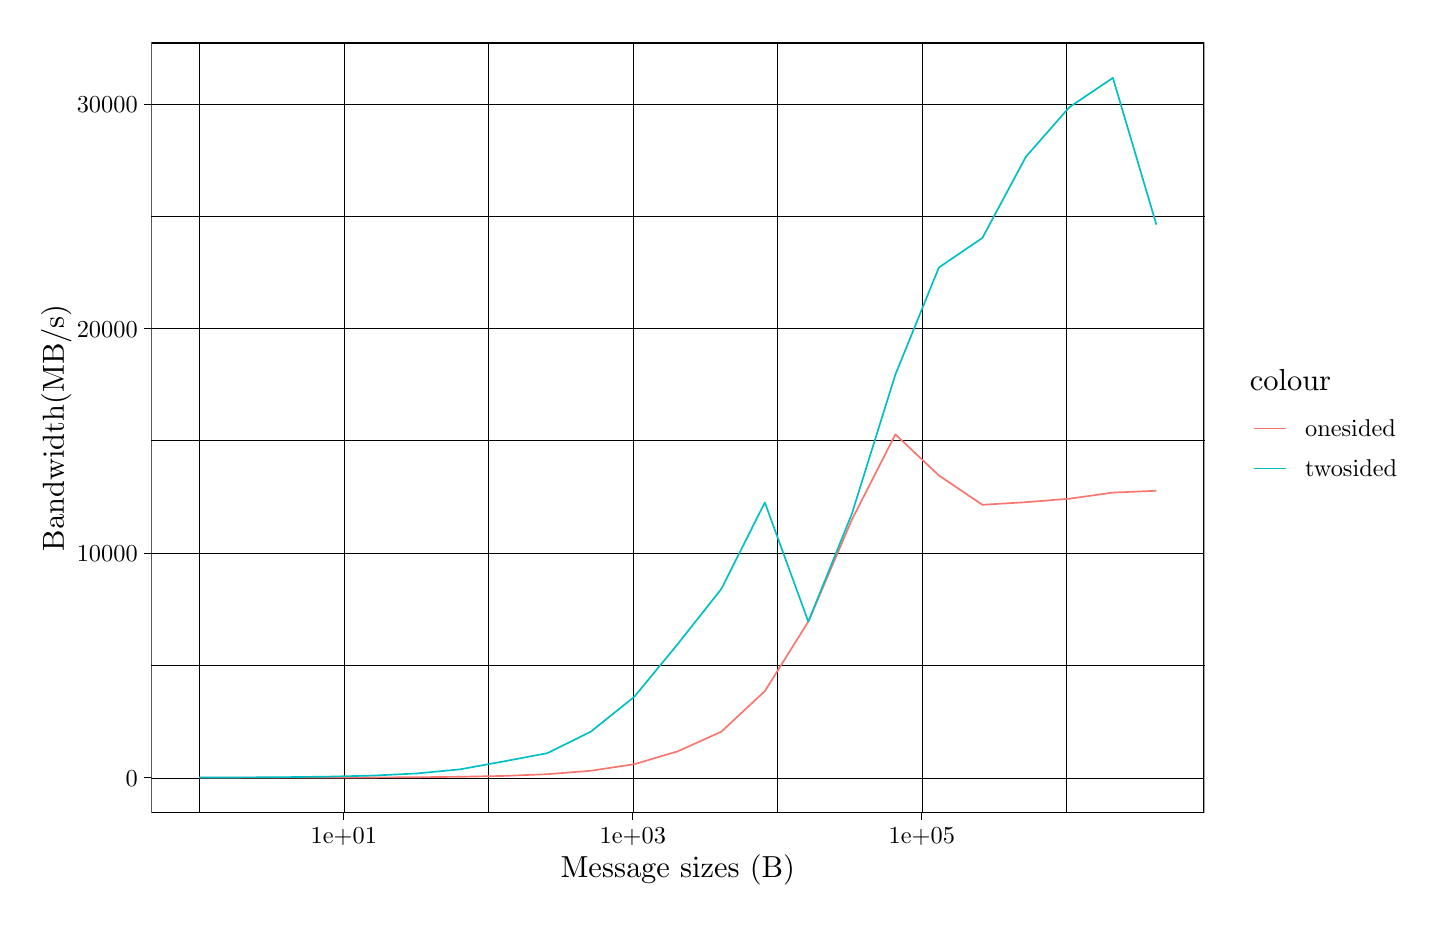
\begin{tikzpicture}[x=1pt,y=1pt]
\definecolor{fillColor}{RGB}{255,255,255}
\path[use as bounding box,fill=fillColor,fill opacity=0.00] (0,0) rectangle (505.89,314.37);
\begin{scope}
\path[clip] (  0.00,  0.00) rectangle (505.89,314.37);
\definecolor{drawColor}{RGB}{255,255,255}
\definecolor{fillColor}{RGB}{255,255,255}

\path[draw=drawColor,line width= 0.6pt,line join=round,line cap=round,fill=fillColor] (  0.00,  0.00) rectangle (505.89,314.37);
\end{scope}
\begin{scope}
\path[clip] ( 44.71, 30.72) rectangle (425.15,308.87);
\definecolor{fillColor}{RGB}{255,255,255}

\path[fill=fillColor] ( 44.71, 30.72) rectangle (425.15,308.87);
\definecolor{drawColor}{RGB}{0,0,0}

\path[draw=drawColor,line width= 0.0pt,line join=round] ( 44.71, 83.93) --
	(425.15, 83.93);

\path[draw=drawColor,line width= 0.0pt,line join=round] ( 44.71,165.05) --
	(425.15,165.05);

\path[draw=drawColor,line width= 0.0pt,line join=round] ( 44.71,246.18) --
	(425.15,246.18);

\path[draw=drawColor,line width= 0.0pt,line join=round] ( 62.01, 30.72) --
	( 62.01,308.87);

\path[draw=drawColor,line width= 0.0pt,line join=round] (166.45, 30.72) --
	(166.45,308.87);

\path[draw=drawColor,line width= 0.0pt,line join=round] (270.90, 30.72) --
	(270.90,308.87);

\path[draw=drawColor,line width= 0.0pt,line join=round] (375.34, 30.72) --
	(375.34,308.87);

\path[draw=drawColor,line width= 0.1pt,line join=round] ( 44.71, 43.36) --
	(425.15, 43.36);

\path[draw=drawColor,line width= 0.1pt,line join=round] ( 44.71,124.49) --
	(425.15,124.49);

\path[draw=drawColor,line width= 0.1pt,line join=round] ( 44.71,205.62) --
	(425.15,205.62);

\path[draw=drawColor,line width= 0.1pt,line join=round] ( 44.71,286.74) --
	(425.15,286.74);

\path[draw=drawColor,line width= 0.1pt,line join=round] (114.23, 30.72) --
	(114.23,308.87);

\path[draw=drawColor,line width= 0.1pt,line join=round] (218.67, 30.72) --
	(218.67,308.87);

\path[draw=drawColor,line width= 0.1pt,line join=round] (323.12, 30.72) --
	(323.12,308.87);
\definecolor{drawColor}{RGB}{248,118,109}

\path[draw=drawColor,line width= 0.6pt,line join=round] ( 62.01, 43.37) --
	( 77.73, 43.37) --
	( 93.45, 43.38) --
	(109.17, 43.40) --
	(124.89, 43.44) --
	(140.61, 43.52) --
	(156.33, 43.68) --
	(172.05, 43.99) --
	(187.77, 44.62) --
	(203.49, 45.86) --
	(219.21, 48.23) --
	(234.93, 52.89) --
	(250.65, 59.97) --
	(266.37, 74.62) --
	(282.09, 99.76) --
	(297.81,136.55) --
	(313.54,167.41) --
	(329.26,152.56) --
	(344.98,141.96) --
	(360.70,142.90) --
	(376.42,144.17) --
	(392.14,146.37) --
	(407.86,147.03);
\definecolor{drawColor}{RGB}{0,191,196}

\path[draw=drawColor,line width= 0.6pt,line join=round] ( 62.01, 43.41) --
	( 77.73, 43.45) --
	( 93.45, 43.55) --
	(109.17, 43.74) --
	(124.89, 44.12) --
	(140.61, 44.88) --
	(156.33, 46.38) --
	(172.05, 49.24) --
	(187.77, 52.21) --
	(203.49, 59.98) --
	(219.21, 72.60) --
	(234.93, 91.67) --
	(250.65,111.55) --
	(266.37,142.79) --
	(282.09, 99.74) --
	(297.81,138.67) --
	(313.54,189.01) --
	(329.26,227.70) --
	(344.98,238.38) --
	(360.70,267.72) --
	(376.42,285.64) --
	(392.14,296.23) --
	(407.86,243.17);
\definecolor{drawColor}{RGB}{0,0,0}

\path[draw=drawColor,line width= 0.6pt,line join=round,line cap=round] ( 44.71, 30.72) rectangle (425.15,308.87);
\end{scope}
\begin{scope}
\path[clip] (  0.00,  0.00) rectangle (505.89,314.37);
\definecolor{drawColor}{RGB}{0,0,0}

\node[text=drawColor,anchor=base east,inner sep=0pt, outer sep=0pt, scale=  0.88] at ( 39.76, 40.33) {0};

\node[text=drawColor,anchor=base east,inner sep=0pt, outer sep=0pt, scale=  0.88] at ( 39.76,121.46) {10000};

\node[text=drawColor,anchor=base east,inner sep=0pt, outer sep=0pt, scale=  0.88] at ( 39.76,202.58) {20000};

\node[text=drawColor,anchor=base east,inner sep=0pt, outer sep=0pt, scale=  0.88] at ( 39.76,283.71) {30000};
\end{scope}
\begin{scope}
\path[clip] (  0.00,  0.00) rectangle (505.89,314.37);
\definecolor{drawColor}{RGB}{0,0,0}

\path[draw=drawColor,line width= 0.3pt,line join=round] ( 41.96, 43.36) --
	( 44.71, 43.36);

\path[draw=drawColor,line width= 0.3pt,line join=round] ( 41.96,124.49) --
	( 44.71,124.49);

\path[draw=drawColor,line width= 0.3pt,line join=round] ( 41.96,205.62) --
	( 44.71,205.62);

\path[draw=drawColor,line width= 0.3pt,line join=round] ( 41.96,286.74) --
	( 44.71,286.74);
\end{scope}
\begin{scope}
\path[clip] (  0.00,  0.00) rectangle (505.89,314.37);
\definecolor{drawColor}{RGB}{0,0,0}

\path[draw=drawColor,line width= 0.3pt,line join=round] (114.23, 27.97) --
	(114.23, 30.72);

\path[draw=drawColor,line width= 0.3pt,line join=round] (218.67, 27.97) --
	(218.67, 30.72);

\path[draw=drawColor,line width= 0.3pt,line join=round] (323.12, 27.97) --
	(323.12, 30.72);
\end{scope}
\begin{scope}
\path[clip] (  0.00,  0.00) rectangle (505.89,314.37);
\definecolor{drawColor}{RGB}{0,0,0}

\node[text=drawColor,anchor=base,inner sep=0pt, outer sep=0pt, scale=  0.88] at (114.23, 19.71) {1e+01};

\node[text=drawColor,anchor=base,inner sep=0pt, outer sep=0pt, scale=  0.88] at (218.67, 19.71) {1e+03};

\node[text=drawColor,anchor=base,inner sep=0pt, outer sep=0pt, scale=  0.88] at (323.12, 19.71) {1e+05};
\end{scope}
\begin{scope}
\path[clip] (  0.00,  0.00) rectangle (505.89,314.37);
\definecolor{drawColor}{RGB}{0,0,0}

\node[text=drawColor,anchor=base,inner sep=0pt, outer sep=0pt, scale=  1.10] at (234.93,  7.44) {Message sizes (B)};
\end{scope}
\begin{scope}
\path[clip] (  0.00,  0.00) rectangle (505.89,314.37);
\definecolor{drawColor}{RGB}{0,0,0}

\node[text=drawColor,rotate= 90.00,anchor=base,inner sep=0pt, outer sep=0pt, scale=  1.10] at ( 13.08,169.80) {Bandwidth(MB/s)};
\end{scope}
\begin{scope}
\path[clip] (  0.00,  0.00) rectangle (505.89,314.37);
\definecolor{fillColor}{RGB}{255,255,255}

\path[fill=fillColor] (436.15,142.34) rectangle (500.39,197.26);
\end{scope}
\begin{scope}
\path[clip] (  0.00,  0.00) rectangle (505.89,314.37);
\definecolor{drawColor}{RGB}{0,0,0}

\node[text=drawColor,anchor=base west,inner sep=0pt, outer sep=0pt, scale=  1.10] at (441.65,183.22) {colour};
\end{scope}
\begin{scope}
\path[clip] (  0.00,  0.00) rectangle (505.89,314.37);
\definecolor{fillColor}{RGB}{255,255,255}

\path[fill=fillColor] (441.65,162.29) rectangle (456.10,176.74);
\end{scope}
\begin{scope}
\path[clip] (  0.00,  0.00) rectangle (505.89,314.37);
\definecolor{drawColor}{RGB}{248,118,109}

\path[draw=drawColor,line width= 0.6pt,line join=round] (443.10,169.52) -- (454.66,169.52);
\end{scope}
\begin{scope}
\path[clip] (  0.00,  0.00) rectangle (505.89,314.37);
\definecolor{drawColor}{RGB}{248,118,109}

\path[draw=drawColor,line width= 0.6pt,line join=round] (443.10,169.52) -- (454.66,169.52);
\end{scope}
\begin{scope}
\path[clip] (  0.00,  0.00) rectangle (505.89,314.37);
\definecolor{fillColor}{RGB}{255,255,255}

\path[fill=fillColor] (441.65,147.84) rectangle (456.10,162.29);
\end{scope}
\begin{scope}
\path[clip] (  0.00,  0.00) rectangle (505.89,314.37);
\definecolor{drawColor}{RGB}{0,191,196}

\path[draw=drawColor,line width= 0.6pt,line join=round] (443.10,155.06) -- (454.66,155.06);
\end{scope}
\begin{scope}
\path[clip] (  0.00,  0.00) rectangle (505.89,314.37);
\definecolor{drawColor}{RGB}{0,191,196}

\path[draw=drawColor,line width= 0.6pt,line join=round] (443.10,155.06) -- (454.66,155.06);
\end{scope}
\begin{scope}
\path[clip] (  0.00,  0.00) rectangle (505.89,314.37);
\definecolor{drawColor}{RGB}{0,0,0}

\node[text=drawColor,anchor=base west,inner sep=0pt, outer sep=0pt, scale=  0.88] at (461.60,166.49) {onesided};
\end{scope}
\begin{scope}
\path[clip] (  0.00,  0.00) rectangle (505.89,314.37);
\definecolor{drawColor}{RGB}{0,0,0}

\node[text=drawColor,anchor=base west,inner sep=0pt, outer sep=0pt, scale=  0.88] at (461.60,152.03) {twosided};
\end{scope}
\end{tikzpicture}

	\caption{1 node, bw, cpu-cpu, flush-local, create window, one-sided, two-sided comparisons}
\end{figure}

\end{document}
